\documentclass[a4paper,11pt,oneside]{article}

\usepackage[greek,english]{babel}
\usepackage{textgreek}
\usepackage[textwidth=3cm,margin=1.2cm,columnsep=1cm,bottom=2cm, top=1.8cm]{geometry}
\usepackage{graphicx}
\usepackage{xcolor}
\usepackage{booktabs}
\usepackage{tcolorbox}
\usepackage{color}
\usepackage[linktocpage,colorlinks=true,linkcolor= {red!50!black}, urlcolor=black, citecolor=blue!90, pdfborder={2 1 0}]{hyperref}
\usepackage{hyperref}
\usepackage{amsmath}
\usepackage{float}
\usepackage{fancyhdr}
\usepackage{refcount}
\usepackage{longtable}
\usepackage{array}
\usepackage{tabularx}
\usepackage{colortbl} 
\usepackage{subcaption}
\usepackage{caption}
\usepackage[numbib,nottoc]{tocbibind}
\usepackage{fancyhdr}
\usepackage{placeins}
\usepackage{algorithm2e}
%TIMS ----------------------------------------------
\usepackage[bottom]{footmisc}
\usepackage{rotating}
\usepackage{amsmath}
\usepackage{amsthm}
\usepackage{amsfonts}
\usepackage{amssymb}
\usepackage{mathrsfs}
\usepackage{fancyhdr}
\usepackage{longtable}
\usepackage{pdfpages}
\usepackage{pdflscape}
\usepackage{array}
\usepackage{tabularx}
\usepackage{colortbl} 
\usepackage{tcolorbox}
\usepackage{etoolbox}
\patchcmd{\thebibliography}{*}{}{}{}
\usepackage{multicol}
%\usepackage{algorithm}
\usepackage{makecell}
\usepackage{algpseudocode}
%\usepackage{program} 
\usepackage[titletoc,title]{appendix}
\usepackage{color}
\usepackage{tabu}
\usepackage{booktabs}
\usepackage{tcolorbox}
\tcbuselibrary{breakable}
\usepackage{float}
\usepackage{graphicx}
\usepackage{titlesec}
%\usepackage[linktocpage,colorlinks=true,linkcolor= {red!50!black}, urlcolor=grey, citecolor=blue!90, pdfborder={2 1 0}]{hyperref}
\usepackage[capitalize]{cleveref} 

\usepackage{svg}


%MINE ----------------------------------------------

\usepackage{xargs}                      % Use more than one optional parameter in a new commands
\usepackage[colorinlistoftodos,prependcaption,textsize=tiny]{todonotes}
\newcommandx{\unsure}[2][1=]{\todo[linecolor=red,backgroundcolor=red!25,bordercolor=red,#1]{#2}}
\newcommandx{\change}[2][1=]{\todo[linecolor=blue,backgroundcolor=blue!25,bordercolor=blue,#1]{#2}}
\newcommandx{\info}[2][1=]{\todo[linecolor=OliveGreen,backgroundcolor=OliveGreen!25,bordercolor=OliveGreen,#1]{#2}}
\newcommandx{\improvement}[2][1=]{\todo[linecolor=Plum,backgroundcolor=Plum!25,bordercolor=Plum,#1]{#2}}
\newcommandx{\thiswillnotshow}[2][1=]{\todo[disable,#1]{#2}}

\newcommand{\myol}[2][3]{{}\mkern#1mu\overline{\mkern-#1mu#2}}
\newenvironment{technicaldoc}

%TIMS ----------------------------------------------



\tcbset{tab2/.style={fonttitle=\bfseries,fontupper=\normalsize\sffamily}}
\newcolumntype{Y}{>{\raggedleft\arraybackslash}X}



% GRAPHICS HANDLING ----------------------------------------------
\setcounter{secnumdepth}{4}

\titleformat{\paragraph}
{\normalfont\normalsize\bfseries}{\theparagraph}{1em}{}
\titlespacing*{\paragraph}
{0pt}{3.25ex plus 1ex minus .2ex}{1.5ex plus .2ex}


\titleformat*{\section}{\LARGE\bfseries}
\titleformat*{\subsection}{\Large\bfseries}
\titleformat*{\subsubsection}{\large\bfseries}
\titleformat*{\paragraph}{\large\bfseries}
\titleformat*{\subparagraph}{\large\bfseries}


\colorlet{linkequation}{blue!90!}%
\makeatletter
\creflabelformat{equation}{%
	\textup{%
		\hypersetup{
			linkcolor=linkequation,
			linkbordercolor=linkequation,
		}%
		(#2#1#3)%
	}%
}


% OTHER SET-UP ---------------------------------------------------

\pagestyle{fancy}
\lhead{\rightmark}
\chead{}
\rhead{\thepage}
\cfoot{}

\setlength{\topmargin}{0.1cm}
\setlength{\headsep}{1cm}
\setlength{\textwidth}{15.0cm}
\setlength{\headwidth}{15.0cm}
\setlength{\headheight}{14pt}
\setlength{\textheight}{22cm}
\setlength{\oddsidemargin}{0.55cm}
\setlength{\evensidemargin}{0cm}
\setlength{\parindent}{0pt}
\setlength{\extrarowheight}{10pt}

\newcommand{\setlinespacing}[1]
{\renewcommand{\baselinestretch}{#1}\small\normalsize}

\allowdisplaybreaks[1]

% THEOREM STYLES -------------------------------------------------

\theoremstyle{plain}
\newtheorem{thm}{Theorem}%[chapter]
\newtheorem{prop}[thm]{Proposition}
\newtheorem{cor}[thm]{Corollary}
\newtheorem{con}[thm]{Conjecture}
\newtheorem{lem}[thm]{Lemma}
\theoremstyle{definition}
\newtheorem{defn}[thm]{Definition}
\newtheorem{ass}[thm]{Assumption}
\newtheorem{exam}[thm]{Example}
\usepackage[font=small,labelfont=bf]{caption}
\DeclareCaptionFont{tiny}{\tiny}
\usepackage{caption}
\captionsetup{font=footnotesize}
%\renewcommand{\thesection}{\Roman{section}} 
%\renewcommand{\thesubsection}{\Roman{section}. \Roman{subsection}}
\usepackage{listings}
\usepackage{blindtext}
\lstset{basicstyle=\small\ttfamily,
	columns=flexible,
	breaklines=true}


% MACRO DEFINITIONS ----------------------------------------------
\setcounter{tocdepth}{4}
% Place your personal macro definitions here.

%\usepackage{hyperref}

%\usepackage[landscape]{geometry}


% PREAMBLE -------------------------------------------------------
\title{Master of Science in Statistics\\ Dissertation: Draft \#1\\[2mm] \textbf{Title \\[0.6cm]}

\includegraphics[scale=1]{UCT-logo.pdf}}
\author{\textbf{Joel da Costa}\\[0.18cm] Supervisor: A/Prof. T. Gebbie \\[0.3cm]
Statistics,\\
Department of Statistical Sciences,\\
University of Cape Town, Rondebosch}%\\[0.25cm]
%\\} %width=2.7cm
\date{2017}

\begin{document} 
\vspace{-7cm}
\maketitle \setlinespacing{1}
\abstract{We consider pattern prediction of financial time-series data. The algorithm framework and workflow is developed and proved on daily sampled OHLCV (open-high-low-close-volume) time-series data for JSE equity markets. The input patterns are based on input data vectors are equal size data windows pre-processed into a sequence of daily, weekly and monthly sampled feature measurement changes (here log feature fluctuations). The data processing is split into at online batch processed step where data is compressed using a stacked autoencoder (SAE) via unsupervised learning, and then batch supervised learning is carried out using the data-compression algorithm with the output being a pattern sequence of measured time-series feature fluctuations (log differenced data) in the future (ex-post) from the training and validation data. Weight initializations for these networks are implemented with Restricted Boltzmann Machine (RBM) pre-training, and variance based initializations. The historical simulation is then run using an online feedforward neutral network (FNN) initialised with the weights from the online training and validation step. The validity of results is considered under a rigorous assessment of backtest overfitting (Combinatorially Symmetrical Cross Validation), and the results are then considered in terms of test for statistical arbitrage with simple correction for transaction costs.}\\
\todo{this will need to be rewritten once everything is finalised}

\noindent\textbf{Keywords:} online learning, feedforward neural network, restricted boltzmann machine, stacked autoencoder, pattern prediction, JSE, non-linear, financial time series, combinatorially symmetrical cross validation, backtest overfitting


\newpage

%--------------------------------------------------------------------------------------------------------------------------------------
% CONTENT --------------------------------------------------------
\tableofcontents

\listoffigures

\listoftables

\newpage

%____________________________________________________________________
\part[\large{Online non-linear prediction of financial time-series patterns}]{\Huge\selectfont{Online non-linear prediction of financial time-series patterns}}



\section{Introduction}\label{Introduction}

\todo{may need to add some appropriate in this section}


This dissertation explores several ideas for the purposes of effective and valid stock price prediction, and suggests a novel approach to the combination of techniques. The first part of the implementation focuses on the training of deep neural networks, and combines usage of several well known designs for data reduction, deep learning and online learning. The aim here is to produce a deep learning model that is able to effectively produce stock price predictions in an online process, using data reduction of high dimensional finance data in order to achieve better results. 
~\\\newline
The second part of the paper focuses on whether the model can be trained such that it does not succumb to backtest overfitting, namely by using methods suggested by Bailey et al. \cite{BailyPBO} in order to calculate the likelihood of overfitting having occurred. As they've noted, and discussed more fully in \ref{lr_backtesting}, backtesting overfitting for trading strategies have become problematically widespread in financial literature. Here we investigate how more rigorous validation techniques can be applied to deep learning models in order to avoid such overfitting. Further validation takes place in assessing the potential profitability of the model in a live market.
~\\\newline
The literature review in chapter \ref{lr_LiteratureReview} has a fuller discussion of work that has been done to precede the various techniques which have been implemented. A brief introduction to technical analysis in the financial sector, with it's perspective and history, is discussed and forms the basis for proposing and using the technical analysis methods throughout this paper \ref{lr_TechnicalAnalysis}. The literature review then moves onto covering the usage and history of Neural Networks, which has progressed enourmously in recent times. The section covers both the basic foundations, and also discusses the recent work which has resulted in the widespread use of deep learning models \ref{lr_nn}. This is extended to the coverage of Stacked Autoencoders, and their efficacy in data reduction for complex systems, which has lead them to be pivotal tools in deep learning models \ref{lr_SAE}. Online learning methods are discussed in \ref{lr_OGD} with a coverage of both the historical basis as well as the more recent devopments which have allowed for further improvment in the algorithms. The chapter finishes off with discussing the impact of backtest overfitting and how some notable works developed by Bailey et al. have provided tools with which this may be avoided \ref{lr_backtesting}.
~\\\newline
Chapter \ref{Data} provides the details around the data which has been used in the paper. The chapter starts with describing how the data is processed using log feature fluctuations, and then is expanded to include the fluctuations over rolling window periods. The synthetic data used is generated using Geometric Brownian motion, and is implemented such that each randomly seeded dataset consists of the following stocks:
\begin{itemize}
	\item 3 stocks with an upward trend, and high, medium and low variance
	\item 3 stocks with a downward trend, and high medium and low variance
	\item 3 stocks with a sideways trend, and high medium andlow variance
\end{itemize}
There is a further summary of the real data used: OHLCV data for the JSE ALSI over a period of 20 \unsure{check this} years.
~\\\newline
Chapter \ref{Implementation} provides more indepth details on the algorithms and structures used to implement the dissertation process. The structure of feedforward neural networks is discussed, as well as how they are trained using the backpropagation algorithm, and how that can be applied in a stochastic descent framework \ref{imp_ffn}. The chapter also provides details for how these network weight initializations can impact performance, and how this can be improved with either RBM pre-training (as per \cite{Hinton2}) or through newer variance based techniques \todo{add ref} - this includes the structures and training techniques used for the Stacked Autoencoders \ref{imp_SAE}. How the CSCV techniques suggested by \cite{BailyPBO} are implemented and used to derive a Probability of Backtest Overfitting figure for the full training and testing processes is detailed in \ref{imp_cscv}. The chapter ends with a summary of the full end to end process, from data preparation to the output of a PBO figure in \ref{imp_fullprocess}.
~\\\newline
Chapter \ref{Results} is the final chapter, and discusses the results found from the process. \todo{this will need to be finished once results are known}
\newpage
\section{Literature Review}\label{lr_LiteratureReview}
\subsection{Technical Analysis}\label{lr_TechnicalAnalysis}

Technical analysis is a financial analytical practice that makes use of past price data in order to identify market 
structures, as well as forecast future price movements. The techniques are typically objective methodologies 
which rely solely on past market data (price and volume). They stand in contrast to fundamental analysis, where 
experts will consider a companies operations, management and future prospects in order to arrive at an evaluation. 
The basis of much technical analysis, originally developed through Dow Theory, is the belief that stock market 
prices will move directionally (upwards, downwards or sideways), and that past movements can be used to 
determine these trends  \cite {Murphy}.
\hfill \break 

One of the primary methods in technical analysis is the use of charts in order to identify price patterns. 
These charts will be produced using the available market data and a known design, such as the popular candle-bar 
plot, which can then be compared to historical data to match it to a particular pattern. These patterns are thus 
indicative that the stock is likely to take on a particular price trend, or is in a particular state \cite {Murphy}.  
There is a certain amount of controversy around technical analysis, where many argue that it is contradictory 
to the random walk and weak form efficient market hypotheses, and as such is not valuable or useful \cite {Griffioen}. 
The argument against this, is that technical analysis does not rely on past action to predict the the future, but is 
rather a measure of current trading, and how the market has reacted after similar patterns have occurred in the 
past \cite {Kahn}. Further, even if the analysis is unable to effectively forecast future price trends, it can still be useful 
to exploit trading opportunities in the market \cite{Schwager}.
\hfill \break 

With the advent of processing power becoming cheaply available, there has been an increase in research to 
adapt computing techniques to technical analysis. The breadth and superhuman speed in which systems are 
able to perform technical analysis far outstrips what was possible before, and as such they have become the 
focus of competitive performance for many market participants \cite {Johnson}. To this end, there has been much 
research to apply machine learning algorithms to perform pattern recognition on stock price movements.
\hfill \break

Financial markets have been shown to be complex and adaptive systems, where the effects of interaction 
between participants can be highly non-linear \cite {Arthur}. Complex and dynamic systems such as these may 
often exist at the 'order-disorder border' - they will generate certain non-random patterned and internal organisation, 
which can be assessed and identified, however they will also exhibit a certain amount of randomness in their behaviours, 
or 'chaos' \cite {Crutchfield}. Further, it's been shown that there is enough signal to reconstruct 
the phase space of chaotic systems from singular observations, encouraging that we might be able to perform 
effective technical analysis in the context of financial markets \cite{Packard, Takens}. As a result, trying to identify these patterns and structures is a simultaneously 
reasonable and notoriously difficult goal. While it is often clear in hindsight that the patterns exist, the amount of 
noise and nonlinearity in the system can make prediction challenging.
Fittingly then, neural networks have become a popular choice for modelling within the financial markets. Due to 
their structure, they are able to learn non-linear interactions between their inputs and outputs, with even early research 
showing their ability to achieve statistically significant results, which lends weight to the 
argument against the efficient market hypothesis \cite {Skabar}. 
\hfill \break



\subsection{Neural Networks}\label{lr_nn}

A Neural Network (NN) is a learning model which was originally inspired by the biological mechanisms of neurons 
in brains. The structure is essentially that of a network system, with connected nodes and edges, or ‘neurons’ and 
‘weights‘ in context. The neurons are based on the same idea as synapses as seen in the brain - where a buildup 
of input results in a ‘firing’ of output. The input here is determined by the model’s input (real numbers typically), 
and processed through the weights and activation functions of the neuron, which then results in an output value 
either at an intermediate level, or as the model’s final output. The system ‘learns’ by considering input samples 
sequentially, and adjusting the weights between edges to result in more accurate outputs, which may either be 
classification or regression values. 
\hfill \break 

Structured neural networks that learn to some extent have been around since the second half of the 21st 
century \cite{Schmidhuber}, though have been through several cycles of popularity. The first versions tended to be very simple 
with one one layer of hidden neurons \cite{Ivakhnenko}. It was only later, through the application of 
the backpropagation algorithm, that they started to become more practical and popular \cite{Werbos}.
\hfill \break 

With the rise in popularity, many different network formations were developed and suggested. One of the initial 
suggestions was the conceptually simple Feedforward Neural Network (FNN) as described above - an acyclic
 graph where inputs are processed in a single direction until the output is reached. The other notable earlier model 
 was the Recurrent Neural Network (RNN), which has a cyclic graph instead - this results in a more powerful 
 computational system than the standard FNN, which was shown to be effective quite early on 
\cite{Siegelmann}. The Long Short-Term Memory (LSTM) network was 
 another that used recurrent dynamics, though at a neuron level, in that the neuron is responsible for remembering 
 values for an arbitrary time period \cite{Hochreiter}. Convolutional Neural Networks (CNN) have a non-recurrent structure, 
 but implement separate pooling layers of neurons which consider the adjacent input values for each feature 
 (e.g. pixels next to each other). These have been shown to be incredibly effective at tasks such as image 
 recognition, as elaborated on later.
\hfill \break 

There are three primary learning paradigms used in neural network training - Supervised Learning (SL), 
where the network is trained on inputs with known outputs; Unsupervised Learning (UL), where the network is 
trained to identify unknown structures as an output; and Reinforcement Learning (RL), where environmental
reactions are used as inputs to train a network for certain outputs \cite{Schmidhuber}. While all of these configurations and paradigms 
have their benefits and uses, this paper will largely focus on FNN and RNNs, trained through SL and UL.
\hfill \break 

\subsubsection{Training and Backpropagation}\label{lr_trainingbackprop}

Historically, the crux of neural networks’ popularity has often been based on the development of novel training 
methodologies, and how they have increased performance. In line with this, the Backpropagation (BP) algorithm (as defined in \ref{imp_backprop})
has played a pivotal part: while neural network (or perceptron) models were around long before NN popularity, 
they were largely deemed ineffective, at least in comparison to other available models of the time 
\cite{Minksy}. It was only during the 1980’s that the BP algorithm was applied to NNs, and 
the field started to gain in popularity again \cite{LeCun2, Werbos2}. 
\hfill \break 

Rumelhart et al. showed that the BP algorithm as applied in NNs resulted in useful feature representations 
occuring in hidden layers and the empirical success that resulted thereof \cite{Rumelhart}.  
Shortly after, LeCun et al. applied the BP algorithm to CNNs with adaptive connections. They were able to show 
impressive performance for the time in classifying handwritten images, with the images as a direct input (rather than a feature vector) \cite{LeCun3}.
\hfill \break 

While many improvements were made during this time via gradient descent modifications, the 
models were typically of a shallow nature due to problems encountered trying to train deeper networks. 
Early experiments with deep networks resulted in poor performance due to what is now widely known as the problem 
of either vanishing or exploding gradients \cite{Pascanu}. Essentially, as more layers are added to the network, the backpropagation 
algorithm (with typical activation function neurons), results in error signals that either shrink or grow out of bounds at an 
exponential rate. One of the first suggested and primary solutions to the problem is to perform pre-training on the 
network through unsupervised learning  \cite{Schmidhuber}, which is discussed more fully in \ref{DBN}. Variance based 
weight initialization techniques have grown in popularity in recent years, as discussed in \ref{lr_weight_init}.
\hfill \break 

There were also initial concerns that the BP algorithm as applied to high dimensional neural networks would result 
in the network weights being trapped in local minima if a simple gradient descent was used (e.g. where no small 
changes to the configuration would reduce the average error rate) \cite{LeCun4}. 
However, empirically, this tends not to so problematic, and large networks usually reach solutions of equitable 
performance. More recent research has shown that the solution spaces largely consist of many saddle points, each 
with varying gradients of the features, but which also tend to have similar values of the objective function \cite{Dauphin}. 
Ge et al. have also shown that it is possible to escape saddle points and offer a guaranteed global convergence 
in certain non-convex problems \cite{Ge}.
\hfill \break 

\subsubsection{Activation Functions}\label{lr_activationfunctions}

One of the upfront configuration choices necessary is the activation function, which allows the mapping of input 
to output at the neuron level. There have been many suggestions and experiments with different functions, though 
there are some common features amongst functions which might make them appropriate: Non-linearity allows for 
neural networks to operate as universal approximators, as shown in \cite{Hornik}, continuous differentiability allows for the 
use of gradient descent and whether the function is monotonic has been shown to indicate whether the solution 
can be guaranteed to have a unique periodic solution \cite{Wu}. Lastly, the range of the function (infinite or finite) can impact both the 
stability and efficiency of the training.
\hfill \break 

Some of the most popular functions that have been used are the Sigmoid, TanH, ReLU and Softsign. There have 
been various studies showing the effectiveness of the different activations under varying initialization (or pre-training) 
for weights. Glorot and Bengio noted that the typical Sigmoid and TanH functions performed poorly with standard 
minimization, and result in slower convergence and worse minima, and showed that Softsign with a non-standard 
initialization resulted in quicker convergence \cite{Glorot}. Further research with Bordes \& Bengio found that the 
rectifier (ReLU) functions were  more effective in deep sparse networks compared to the TanH function \cite{Glorot2}.

\subsubsection{Deep Learning}

As noted above, most of the earlier work using neural networks relied on shallow models with few layers. 
However, a resurgence in interest occurred in 2006 after several papers demonstrated the efficacy of 
unsupervised pre-training of networks prior to supervised training. The effect was substantial enough to allow 
much deeper layered networks to be trained than before \cite{Bengio1, Hinton1}.
\hfill \break 
 
 The essential point behind the unsupervised learning was to initialize the weights in the network to sensible 
 values in light of the problem context. The methods used trained each layer to be able to reconstruct the model 
 of the features in the layer below (to a varying degree of accuracy). Sequentially pre-training and combining 
 layers like this, the process generated a deep neural network with appropriate weights. Once done, a final output 
 layer was added and the entire network could then be fine-tuned through backpropagation, without suffering 
 such performance degradation through vanishing or exploding gradients \cite{Hinton1, Ranzato1, Hinton2}. This is 
 expanded up further in \ref{DBN}. Le Roux and Bengio were able to show that within the DBNs produced by 
 Hinton \cite{Hinton1}, adding hidden nodes resulted in strictly improved modelling capabilities, and they suggested 
 that increasing the number of layers is likely to result in increased representational ability (subject to efficacy of 
 previous layers), thus establishing the argument for deep networks in theory as well as practice \cite{LeRoux}.
\hfill \break 

FNNs had been shown to be effective in modelling high dimensional data even prior to the breakthroughs in 
deep networks \cite{Bengio2}, so it fits that the deep networks were shown to be extremely effective in high dimensional 
data classification. Early implementations shown increased efficacy in handwriting recognition, as well as pedestrian 
recognition \cite{Sermanet}. When it came to data types such as sound and images, CNNs were implemented on several 
occasions with record breaking model performances in recognition, notably in ImageNet and WaveNet \cite{ImageNet, WaveNet}.
\hfill \break 

As more research into deep networks was conducted, it became apparent that with large enough datasets, the
 layerwise pre-training of networks was not actually necessary to achieve high performance standards 
 \cite{ImageNet, Glorot2, Ciresan}. When training for long enough, it was reported that the pre-training offered little to no 
 benefit, though these models were typically using datasets far larger than were attempted before (as a result of
  hardware improvements enabling as much). While these results did require that certain attention was paid to the 
  initialization, as well as the use of nonlinear activation units, it did suggest that pre-training largely acted as a prior 
  which may not be necessary if large enough labelled datasets are available \cite{Bengio3}. Naturally, pre-training was still 
  implemented to prevent overfitting in smaller datasets.
\hfill \break 

\subsubsection{Weight Initialization Improvements}\label{lr_weight_init}

One of the more critical innovations to allow effective training of deep networks without using pre-training was the development of more sophisticated techniques for weight initialization. One of the first and most popular of these was presented by Glorot and Bengio for use in Sigmoid based networks, 
and is commonly referred to as Xavier/Glorot initialization \cite{Glorot}. The technique is layer specific and based on a linear activation
hypothesis, such that the initial weights would maintain the same variance for input for information that is passed backwards as in 
accordance with the nature of the activation function. While the assumption of linearity is not entirely correct, they point out that as the 
start of the learning process, it is typically the area of the activations where the gradient is close to 1 which is being explore, thus intially approximating 
a linear effect. The effect is a technique that increases learning efficacy and optima found \cite{Glorot}. \newline

This same methodology was extended for the ReLU activation by He et. al, once again based on the linearity hypothesis around the 
relevant activation function, (Parametric Rectified Linear Units in this case). The combination of ReLU activations, which are computationally inexpensive and do not suffer from learning slowdown, as well as an effective weight initialization technique such that pretraining was not necessary produced a seminal FNN training framework. He et al. were able to 
achieve state of the art performance and produced the best known error rate at the time on the ImageNet dataset \cite{He}. The efficacy of these techniques has established 
them as norms in the training of deep neural networks.


\subsection{Stacked Autoencoders}\label{lr_SAE}

\subsubsection{High Dimensional Data Reduction}\label{HDDR}

As noted, machine learning techniques have been shown to be extremely effective at modelling non-linear inputs 
to outputs - neural networks have even been shown to be universal function approximators in this regard \cite{Hornik}. 
More traditional statistical models will typically process the available feature data to select the most significant 
features to be used in the model once it’s defined - evident in a processes such as subset selection \cite{Schaefer}. 
Machine learning techniques are no different in this regard, and feature data will typically be transformed to smaller 
observations of more significance prior to being used as input to a model, such as the neural networks described above.
\hfill \break 

Financial data, in line with the complex and dynamic system that it represents, is often of a very high dimensional 
nature, which offers opportunities through more sophisticated analysis, but also introduces the curses of
 dimensionality \cite{Donoho}. The increased dimensionality can result in higher processing complexities when needing to 
 do basic tasks such as estimating a covariance matrix (a commonplace necessity in finance), as well as increase 
 the risk of incorrect assumptions based on spurious variable collinearity \cite{Fan1}. Noise accumulation in high 
 dimensional data can create further problems, resulting in problems performing variable selection and ultimately 
 having a large impact on classification and regression models \cite{Fan2}.
\hfill \break 

Time series data can introduce its own set of challenges - there is often not enough data available to understand 
and predict the process \cite{Fama}, the time variable dependence creates complexity in how much past 
data to consider at any point, and the data is typically non-stationary \cite{Langkvist}. Thus, high dimensional time 
series data (which many financial problems focus on), require careful consideration on how to handle their inputs 
and analysis.
\hfill \break 

Deep learning techniques are a natural choice in this context, and much research has been done to show their 
(varying) efficacy on time series data. The most successful of these models have been ones which modify deep 
learning techniques to incorporate the temporal aspect of the data (e.g. Conditional Restricted Boltzmann 
Machines or Recurrent Neural Networks), rather than static, and those which have performed feature selection
 processes rather than operating on the raw data (e.g. Auto-encoders)  \cite{Langkvist}. 
 \hfill \break 
 
 
Two of the seminal pieces of research that have lead to the resurgence in machine learning and deep learning 
were the algorithms for training deep belief networks \cite{Hinton1}, as well as the usage of stacked auto-encoders
\cite{Ranzato1, Bengio1}. 

 
\subsubsection{Deep Belief Networks}\label{DBN}
 
 Autoencoders were suggested by Hinton et. al as a method of transforming high dimensional 
 data to lower dimensional input vectors, in order to alleviate some of the problems detailed above, and increase 
 performance of deep belief networks \cite{Hinton2}.
\hfill \break 

One of the more prominent classical techniques for dimension reduction is principal components analysis (PCA), 
which uses linear algebra to find the directions of greatest variance, and represent the observation samples 
features along each of these directions, thus maximising the variational representation. Hinton et al. show that 
autoencoders are a nonlinear generalization of PCA. The structure and training algorithms of the autoencoder 
show it to be a specialised neural network - there is a multilayer encoder network which is able to transform to a 
lower dimension, and a symmetrical decoder network to recover the data from the code as represented in Figure \ref{figure-DBN-RBM}. As with 
neural networks, the gradient weights can be trained through the feedforward and backpropagation algorithms.  
\hfill \break 

The primary challenge presented here was the initial weighting of the networks - with large initial weights the 
autoencoder will often find a poor local minima, and with small initial weights the gradients are too small to 
effectively train deep layered networks. The critical suggestion by Hinton et al. was to used layered Restricted 
Boltzmann Machines (RBM) in order to initialise the weights. For each layer of the desired autoencoder, a RBM is 
formed and trained with the previous layer (or RBM) \cite{Hinton3}. Once all the layers have been 
trained in this way, they are mirrored to form the decoder network. This then forms the initial weights to be fine 
tuned further, as per the Fine-tuning step in \ref{figure-DBN-RBM}. They showed the deep autoencoder networks were significantly more 
effective than PCA or shallow autoencoders on multiple dataset types. 
 \hfill \break 
 
\begin{figure}
\centering 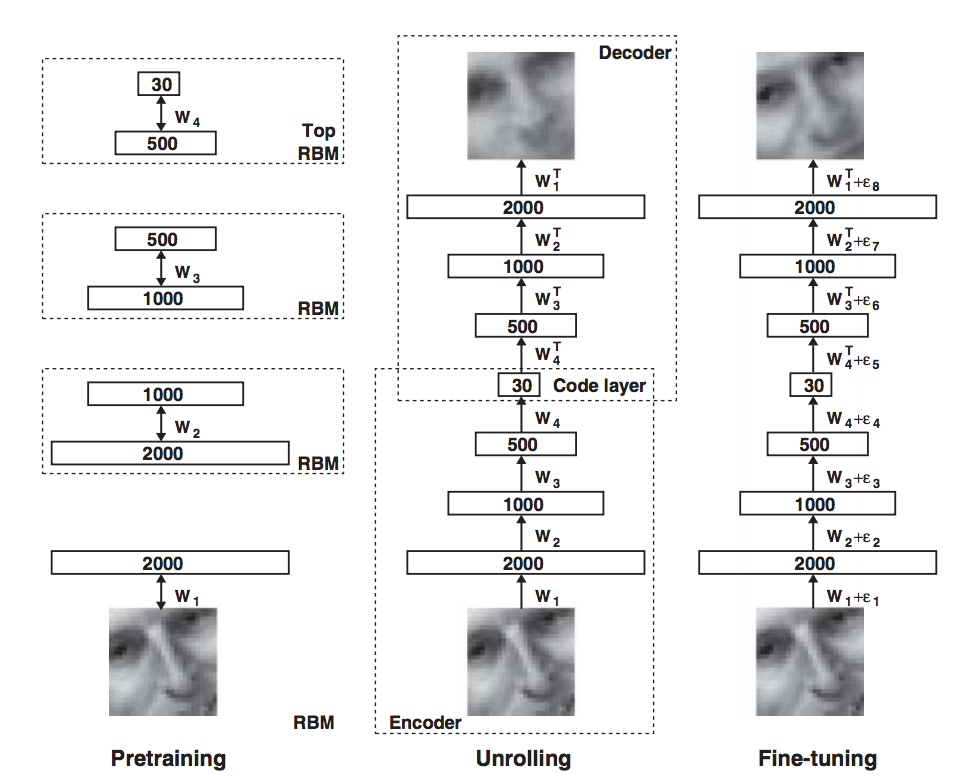
\includegraphics[scale=0.5]{images/DBN-RBM-process.png}
 \caption{The Autoencoder training steps \cite{Hinton2}}
 \label{figure-DBN-RBM}
 \end{figure}
 
\subsubsection{Stacked Denoising Autoencoders}\label{lr_SDAE}

 The second important piece of work was the development of a denoising autoencoder (DAE), by Vincent  et al. \cite{Vincent}. 
 One of the problems identified in the DBN model (and those similar), is that if the encoder dimensions were too high, 
 it is likely that the encoder would learn a trivial encoding - essentially creating a “copy the input” model. The one way
  of tackling this issue is to constrain the representation with bottlenecks and sparse autoencoder layers, which can be seen in figure  \ref{figure-DBN-RBM}.
  \hfill \break 

Vincent et al. explore a very different approach to the problem, which was to develop an implementation of 
autoencoder which focused on partially corrupting the input, and so force the network to ‘denoise’ it. The theory 
here is based on two ideas - the first, is that a higher dimensional representation should be robust to partial 
corruption of the input data; and the second is that the denoising process will force model focus to shift to 
extracting useful features from the input.
 \hfill \break 

The algorithms and structures are largely the same as described for DBNs above, with the key difference 
being that the model is trained to reconstruct the original input, but only using a corrupted version of the input 
(where noise has been added to it), and so is forced to learn smarter feature mappings and extractions. 
The DAE suggested then is a stochastic variant of the autoencoder, which has the benefit of being able to 
implement higher dimensional representations without risking training of a trivial identity mapping. Notably, 
in the Stacked Denoising Autoencoder (SDAE) formation, only the initial input is corrupted (as opposed to the 
input from layer to layer). It was shown that the SDAE model outperformed previous AE and DBN networks on 
numerous benchmark datasets \cite{Vincent} . 

\subsubsection{Pre-training}

The methods described above follow a similar approach: greedy layer-wise unsupervised pre-training in order to 
determine initial weights, followed by supervised fine tuning to arrive at the final model. It is shown numerous times, 
that the pretraining process can result in significant performance gains \cite{Vincent}. However it is not immediately apparent, 
given the nature of backpropagation algorithms and the like, why this is the case. Erhan et al. performed 
extensive empirical simulations in order to suggest an explanation to the mechanism of pre-training \cite{Erhan}.
 \hfill \break 

While their results were not entirely conclusive, they did lend themselves to a reasonable hypothesis: 
the unsupervised pre-training results in a form of regularization on the model - variance is minimized, and the 
bias introduced acts as a prior to direct the model configuration towards a sample space that is effective for the unsupervised 
learning generalization optimisations.

\subsubsection{Time Series Applications}

The autoencoder papers reviewed so far in this section derive their results primarily from classification problems, 
and so do not necessarily account for the problems involved with time series as described in \ref{HDDR}. Due to 
the inherent difficulties with predictions in the financial system, it can sometimes be unclear if the shortcoming in 
results is due to this system complexity or if the methodologies used are unsuited for the purpose. In light of this 
it is worth pointing out that Stacked Autoencoder (SAE) implementations have been shown to be effective in many
 time series systems.  
 \hfill \break 

Lv et al.  implemented a deep learning SAE model using the methods described in \ref{lr_SDAE} in order to 
predict traffic flow at various time intervals (15, 30, 45 and 60 minutes) - a problem not so structurally dissimilar 
from what will be presented in this paper \cite{Lv}. They were able to show that the deep SAE was able to offer prediction 
results which were both objectively good and also persistently outperformed the comparison models used 
(backpropagation neural network, random walk forecast, support vector machine and a radial basis function 
neural network).
\hfill \break 

In a review of unsupervised feature learning and deep learning methods on time series, Langkvist et al. noted that 
the use of autoencoders, either as a technique in themselves, or as an auxiliary technique to models 
such as convolutional neural networks, were able to offer performance increases in areas such as video analysis, 
motion capture data and bacteria identification \cite{Langkvist}.
 
\subsubsection{Financial Applications}

There have of course also been successful applications of stacked autoencoders and deep learning models in 
finance as well. Takeuchi et al. performed some earlier work showing the use of autoencoders when applied to a 
momentum trading strategy. They implemented an RBM pre-trained DBN as per \ref{DBN}, and assessed the 
networks classification performance for ordinary shares on NYSE, AMEX and Nasdaq. This showed that using a 
DBN network resulted in significant performance increases compared to the standard momentum strategy \cite{Takeuchi}.
\hfill \break 

Zhao et al. used SDAEs and combined them with the bootstrap aggregation ensemble method (‘bagging’) in a 
study of predicting the crude oil price. They compared the proposed model to a variety of benchmarks, including 
standard SAE, bagged and standard feedforward networks and SVRs. The results indicated that the SAE models 
were more accurate, with the bagged SAE model performing the best, though at a significant increase in 
computational costs in comparison to standard SAE \cite{Zhao}.
\hfill \break 

While much of the financial literature has focused on the use of RBM based models, Autoencoders and SAEs have 
recently been gaining popularity in performing feature reduction. Troiano et al. specifically investigate the use of 
different feature reduction models for trend prediction in finance \cite{Troiano}. In line with being primarily 
interested in the effect of feature reduction techniques, rather than the classification performance itself, only an 
SVM model was used to test results. Using various periods from historical S\&P 500 data, they were able to show 
that AE outperformed the RBM model significantly in numerous accuracy measures, and was able to do so at a 
fraction of the training time.
\hfill \break 

Bao et al.  note that the research has been lacking with regards to whether SAEs should be used for 
financial prediction models or not \cite{Bao}. They suggest a novel model which combines Wavelet Transformation, SAEs 
and a Long Short Term Memory (LSTM) network. Using data from several financial exchanges (considering a 
range of ‘developed’ and ‘undeveloped’ markets), they assess the model’s applicability to OHLC prediction. 
Comparing the model to configurations without the SAE layers, and a RNN model as benchmark, they showed 
that the inclusion of SAEs resulted in less volatility and greater accuracy, which in turn offered higher profitabilities 
in a buy-and-hold trading strategy.
\hfill \break 

More novel autoencoder applications have also been attempted, with Hsu suggesting the use of a 
Recurrent Autoencoder for multidimensional time series prediction \cite{Hsu}. There is a clear pattern through the literature 
that the use of AEs and SAEs both by themselves and when used as an assisting technique result in more accurate 
prediction results and less computationally expensive training.

\subsection{Online Learning Algorithms and Gradient Descent} \label{lr_OGD}
\hfill

Most classic machine learning algorithms operate under the assumption that, for all intents and purposes, the 
full dataset has been collected and that the amount of training data for the model is both finite and immediately 
available. However, as the growth of information grows in an exponential fashion, there are numerous areas where
 the expected training data for the model will continue to grow. In these cases it would be disadvantageous to go 
 through the full training and validation process again in order to incorporate the newly available data.
\hfill\break

Online algorithms are designed to offset these issues by adjusting the batch training technique to rather 
repetitively draw on single samples from the data on which the model’s parameters can be adjusted. The benefit 
is that they are able to quickly process a large number of observations and readjust the model, though the 
downfall is that they are not always able to optimize the cost function to the same extent as offline batch 
algorithms \cite{Albers}.
\hfill\break

Bottou and Cun argue that as the size of the dataset grows significantly, online algorithms advantages result in 
them outperforming offline models, despite any initial drawbacks \cite{Bottou}. Previous research had shown that online 
algorithms typically perform as fast as batch algorithms during the ‘search’ phase of parameter optimization, but 
that ‘final’ phase convergence tended to fluctuate around the optima due to the noise present in single sample 
gradients \cite{LeCun, Bottou2}. Bottou and Cun showed in fact, that it is more practical to consider the convergence towards
 the parameters of the optima, rather than the optima itself (as defined by the cost function) - the difference 
 between the learning speed and optimization speed, respectively \cite{Bottou}. Theoretical and empirical findings were 
 presented to show that a stochastic online gradient descent algorithm was able to 
 outperform the batch model for parameter estimation, and was able to asymptotically outperform in the number of 
 samples processed in a time period. The stochastic aspect of the algorithm is related to random observations 
 from batch sample groups being used as the gradient basis. Theoretically, this slows down the convergence, but 
 speeds up the processing speed of each batch - a technique which has later been shown to be generally 
 successful \cite{Shalev, Zhang}. 
 \hfill\break
 
Stochastic gradient descent algorithms have resulted in a fair amount of further research due to their applicability to machine learning 
 and the online benefit, especially in relation to their usage in neural networks.
\hfill\break

\subsection{Gradient Learning Improvements}\label{lr_grad_improv}

\subsubsection{Gradient Adjustments and Regularization}

One of the earlier improvements to convergence rates was the Momentum algorithm, as developed by Tseng \cite{Tseng}. 
As noted, stochastic descent often introduces significant oscillation around an optima, which slows down 
convergence. Momentum reduces this by decreasing movement in directions of high curvature, and  
increasing movement towards directions consistent with previous gradients (this is achieved through combining 
gradient movements in opposite directions).
\hfill\break

There have been several attempts to introduce effective regularization into the SGD process. Bartlett et al. 
presented Adaptive Online Gradient Descent, which implements an adaptive step size through a $\lambda$ 
penalty on the learning rate, which was shown to be nearly optimal in a strong sense \cite{Bartlett}. Langford et al. 
demonstrated a variation named Truncated Gradient, which introduced an enforced weight sparsity parameter. 
The weight sparsity is able to achieve equitable effects to $L_1$ regularization (similar to Lasso Regression). 
They were able to show that implementation performed effective feature reduction, while having little effect on 
performance \cite{Langford}. Other approaches, such as AdaGrad, aim to improve the robustness of gradient training by 
adjusting the updates to parameters according to frequency - e.g. larger updates to infrequent parameters, and 
smaller updates to frequent parameters \cite{Duchi, Zeiler}. 
\hfill\break

\subsubsection{Dropout}

One of the instrumental improvements in further achievements, was to modify the backpropagation 
algorithm using the ‘dropout’ technique, as suggested by Hinton et al \cite{Hinton4}. When training of large networks is 
attempted on small datasets, it often results in overfitting and poor results on out of sample data. Dropout helps 
resolve this by randomly excluding a certain percentage (usually 0.5) of feature detectors on each training iteration. 
The effect is to stop co-adaptations of feature detectors, and by rather training each neuron in a wide variety of 
internal configurations, it forces them to take on more usefully generalizable characteristics (it was noted that this
is not a dissimilar technique to ensemble methods, or bagging). The authors were able to show that the method
resulting in significant improvements on benchmark data sets (e.g. MNIST, CIFAR-10), and that a simpler model 
using dropout was able to achieve near comparable performance for the ImageNet dataset.
\hfill \break 

Goodfellow et al. used the dropout technique as the basis for their ‘maxout’ activation function technique, which 
leverages and improves on dropout’s fast optimisation and accuracy through averaging characteristics. The 
maxout model was shown to achieve state of the art performance on benchmark datasets, as well as have a 
strong theoretical grounding \cite{Goodfellow}. Further work was done by Wang et al., which improved on the dropout 
(and potentially maxout) techniques through fast sampling, resulting in an order of magnitude speedup in
training \cite{Wang2}.
\hfill \break 



\subsubsection{Learning Rate Schedules}

Several more recent approaches look towards learning rate adjustment schedules rather than strategies to alter the 
weight update, as with momentum and the like. A constant learning rate often suffers from one of two problems - 
if set too high, it can cause divergent behaviour in the loss function, though if set too low, it can result in slow 
learning or an inability to escape saddle points effectively. Finding an optimal learning rate requires some degree
of testing, though even then a singular value may fail to achieve the same degree of efficacy as a range of values 
explored throughou the solution space. \newline

Learning rate scheduling has been proposed as a solution to this problem. These methods implement an repetitive cycle 
for the learning rate, such that it is set through a range of values between a mimima and maxima, being adjusted slightly 
with each new epoch. Smith suggests using the Cyclical Learning Rate to achieve this, and points out that part of the benefit 
in learning rate schedules is the ability to jump out of sharp optima points which may not generalise well to unseen data \cite{Smith}. 
It's shown that this implementation can have significant performance effects in reaching either the same optima in fewer epochs or a better 
overall optima, including when used in conjunction with other learning optimizations noted in \ref{lr_grad_improv}. These results were 
shown against standard datasets such as CIFAR-10, CIFAR-100 and Imagent \cite{Smith}. \newline

Similarly, Loshchilov and Hutter, expand on this and present Stochastic Gradient Descent with Warm Restarts \cite{Loshchilov}. The approach is 
implemented similarly, but rather follows an asymmetric cycle from a maximum to a minimum, and then starting once again at the maximum once the set number 
of epochs has passed. They too note the increased performance on CIFAR-10 and CIFAR-100 datasets in reaching optima far quicker, as well as noting the efficacy of the 
learning rate schedule even without implementing the restarts \cite{Loshchilov}.



\subsection{Backtesting and Model Validation} \label{lr_backtesting}
\hfill

Much of financial academic literature is currently facing a problem in terms of validation and verification of results. 
The primary method of going about these ends in the past has been to perform historical simulations, or ‘backtests’ ,
in order to prove profitability of a trading strategy. The recent advances in both technology and the algorithms available 
to construct these strategies has resulted in researchers being able to run so many iterations of a model or strategy
 configuration through these backtests, that its become increasingly difficult to control for spurious results, with some 
 papers suggesting that ‘most published research findings are false’   \cite{Ioannidis}.
\hfill \break 

The standard way of implementing backtests is to split the data into two portions: an In Sample (IS) portion which
 is used to train the model, and an Out of Sample (OOS) portion which is used to test the model and validate results. 
 The problem lies in that millions of different model configurations might be tested, and if more sophisticated test 
 measures are not in place (i.e. not just the standard Neyman-Pearson hypothesis testing framework is implemented), 
 then it is only a matter of time before a false positive result occurs which shows high performance both IS and OOS (i.e. overfitting). 
 The nature of financial data, where there is a low signal-to-noise ratio in a dynamic and adaptive system, and 
 where there is only one true data sequence, makes it difficult to resolve these issues effectively 
\cite{BailyPBO, McLean}.
\hfill \break 

Overfitting is not a novel issue, and has of course been tackled in various literature areas, including machine learning. 
However, in that context, the frameworks are often not suited to the buy/sell with random frequency structure of 
investment strategies. They also do not account for overfitting outside of the output parameters, or take into 
consideration the number of trials attempted. Other methods, such as ‘hold-out’, are arguably still faulty due to researcher 
knowledge while constructing models \cite{Schorfheide}. One of the downfalls of the typical IS-OOS set up in the 
financial context is also that the most recent (and relevant) data will not be able to be used for the model training. 
\hfill \break 

There have been some suggestions to resolve the problem that is occuring in the literature as a result of this - some 
work suggesting new frameworks, which this section will cover, and others which focus on the review process or 
how data and replication procedures are made available \cite{Prado}. While the points made with regard to the review process 
and so on are certainly important, they don't aid with more effective model training for the researcher up front, and 
so will not be covered here.

\subsubsection{Testing Methodologies}\label{lr_cscv}

Considering the issues laid out above, there has been much work to develop alternative approaches to backtesting. 
One of the common approaches to avoid backtest overfitting is the ‘hold-out’ strategy, where a certain portion of 
the dataset is reserved for testing true OOS performance. Numerous problems have been pointed out with this 
approach, including that the data is often used regardless, or that awareness of the movements in the data may, 
consciously or otherwise, influence strategy and test design by the researchers \cite{Schorfheide}. For small samples, 
a hold-out strategy may be too short to be conclusive \cite{Weiss}, and even for large samples it results in the 
most recent data (which is arguably the most pertinent) not being used for model selection \cite{Hawkins, BailyPBO}.
\hfill \break 

There has been work by several authors to try and lay out techniques to try and avert backtest overfitting. 
The Model Confidence Set (MCS), as developed by Hansen et al. \cite{Hansen}, starts with a 
collection of models or configurations, and remove models iteratively according to a defined loss function. 
The confidence set is defined by the remaining models once a non-rejection takes place within the process, and 
these models are considered to be statistically similar within a certain confidence range. MCS is thus able to facilitate 
equitable model selection. However, Aparicio et al. \cite{Aparicio}, showed  that while MCS is a potential strategy, in 
practice is is ineffective due to the inordinate requirement of signal-to-noise necessary to identify true superior 
models, as well as a lack of penalization over the number of trials attempted.
\hfill \break

Bailey et al. \cite{BailyPBO} have developed a more robust approach to backtesting and how overfitting during strategy 
selection might be avoided, called Combinatorially Symmetric Cross-validation (CSCV). Their research defines backtest overfitting as having occurred when the strategy selection which maximizes IS performance systematically underperforms median OOS in comparison to the remaining configurations. They use this definition to develop a framework which measures the probability of such an event occuring, where the sample space is the combined pairs of IS and OOS performance of the available configurations. The probability of backtest overfitting (PBO) is then established as the likelihood of a configuration underperforming the median IS while outperforming IS. 
\hfill \break 

The CSCV methodology provides several important benefits over traditional testing 
frameworks, including the usual K-fold cross validation used in machine learning. By recombining the slices of 
available data, both the training and testing sets are of equal size, which is particularly advantageous when comparing 
financial statistics such as the Sharpe Ratio (SR), which are susceptible to sample size. Additionally, the symmetry 
of the set combinations in CSCV ensure that performance degradation is only as a result of overfitting, and not 
arbitrary differences in data sets. It is pointed out that while CSCV and PBO should be used to evaluate the quality 
of a strategy, they should not be the function on which strategy selection relies, which in itself would result in overfitting.
\hfill \break 

\subsubsection{Test Data Length}
\todo{shorten section?}

The CSCV methodology offers an important but highly generalised framework to assess models and backtest 
overfitting. It doesn’t however indicate which metrics should be used to assess the IS and OOS performance, nor 
any indication on the amount of data needed to do so effectively. One of the noted limitations of the framework is 
that a high PBO indicates overfitting within the group of N strategies, which is not necessarily indicative that none 
of the strategies are skillful - it could be that all of them are. Also, as pointed out, it should not be used as an 
objective function to avoid overfitting, but rather as an evaluation tool. To this end it helps assess overfitting, but 
not necessarily avoid it. 
\hfill \break 

A typical measure of evaluation used for financial models is the Sharpe Ratio (SR), which is the ratio of between 
average excess returns and the returns’ standard deviation - a measure of the return on risk. In the context of 
comparing models, SR is typically expressed annually to allow models with different frequencies to be compared. 
Lo et al. \cite{Lo} show that annulaized SR can be expressed as

\begin{equation}\label{SRAnnual}
SR=\frac{\mu}{\sigma}\sqrt{q}
\end{equation}

Using sample means and deviations, $\hat{\mu}$ and $\hat{\sigma}$, SR can be shown to converge as follows 
(as y $\rightarrow\infty$)

\begin{equation}\label{SRConvergence}
  \hat{SR}  \rightarrow \mathcal {N} [SR,\frac{1 + \frac{SR^2}{2q}}{y}]
\end{equation}

Thus, when using SR estimations, which follow a Normal distribution, it is possible that where the true SR mean is 
zero we may still (with enough configurations attempted) find an SR measurement which optimises IS performance. 
This is shown by Bailey et al. \cite{BaileyBTL}, who propose the non-null probability of selecting an IS strategy with null expected 
performance OOS. Notably, typical methods such as hold-out once again fail, as the number of configurations 
attempted are not recorded. They add a further derivation, thich is the Minimum Backtest Length (MinBTL), ultimately 
showing that

\begin{equation}\label{MinBTL}
MinBTL \approx (\frac{
                                  (1-\gamma)Z^{-1}[1-\frac{1}{N}] + \gamma Z^{-1}[1 -\frac{1}{N}e^{-1}]}
                                  {\overline{E[max_N]}})^2
                                  < \frac{2ln[N]}{\overline{E[max_N]}}^2
\end{equation}

The statistic highlights the relationships between: selecting a strategy with a higher IS SR than expected OOS, 
the number of strategies tested (N), and the number of years tested (y). The equation shows that  as the number 
of strategies tested increases, the minimum back test length much also increase in order to contain the likelihood 
of overfitting to IS SR. 
\hfill \break 

As shown extensively throughout ML literature, increased model complexity and number of parameters is one of 
the primary causes of overfitting. In context of the MinBTL formula, model complexity affects the number of 
configurations that are available and which may be tested, which in turn will increase likelihood of overfitting. 
A lack of consideration, or reporting, of the number of trials makes the potential for overfitting impossible to assess. 
\hfill \break 

Bailey et al. expanded on this view with assessing the impact of presenting overfit models as correct. 
They were able to show that in lieu of any compensation effects (i.e. a series following a Gaussian random walk), 
there is no reason for overfitting to result in negative performance. However, where compensation effects apply 
(e.g. economic/investment cycles, bubble bursts, major corrections etc.), then the inclusion of memory in a strategy
 is likely to be detrimental to OOS performance if overfitting isn’t controlled for \cite{BaileyBTL}.
\hfill \break 

\subsubsection {Sharpe Ratio}

The use of the Sharpe Ratio in financial backtesting is not just an arbitrary or persistent literature choice. 
The statistic offers two benefits: the effectively strategy-agnostic financial information contained, as well as being 
relatable to the t-statistic, and so simple to perform hypothesis testing. The SR ratio (estimate from sample as $\hat{SR}$) 
is defined as

\begin{equation}\label{SR}
  SR=\frac{\mu}{\sigma}
\end{equation}

The t-ratio is defined as 

\begin{equation}\label{tratio}
  t-ratio = \frac{\hat{\mu}}{\hat{\sigma}/\sqrt{T}}
\end{equation}

Evidently, the link heree ratio (though it can be generalized to another statistic with a probabilistic interpretation). Additionally, 
PBO is generally more in line with machine learning literature with the cross validation like approach on time series data.  
\hfill \break 

It should be noted, that the literature detailing usage of the Sharpe ratio for strategy comparison is extensive, with 
numerous variations and methodologies offered \cite{BaileySharpe}. However, the crux of this paper lies 
in whether an online neural network is able to make effective enough predictions that a strategy might use the 
predictions to be profitable. The subtlety here is that we will consider the usage of such forecasting \textit{within} a strategy,
 rather than \textit{as} a strategy itself. In line with this, statistics such as the Sharpe ratio will be used, but not form a critical 
 consideration of the research here as the comparison of strategies will not be the focus.
\hfill \break 

\newpage


\section{Implementation: Data Processing and Generation }\label{Data}
\subsection{Data Processing}\label{data_processing}

The datasets used go through several transformations throughout the training and prediction process:

\begin{itemize}
	\item [1] The raw data is log differenced and aggregated to rolling windows
	\item [2] The transformed data is split into Training and Prediction subsets
	\item [3] The predicted outputs have the scaling and log differencing reversed in order to reconstruct the actual price points
\end{itemize}

\subsubsection{Log Difference Transformation and Aggregation}\label{ldata_og_difference}
All datasets are transformed into log feature fluctuation values, and were then aggregated to include fluctuations over rolling window periods. The log feature fluctuation for timepoint $t$ is calculated using \eqref{eq_logdiff}:
\begin{equation}\label{eq_logdiff}
\texttt{log\_diff\_x}_t = ln(x_t) - ln(x_{t-1})
\end{equation}
This log feature fluctuation,  is processed for each asset's closing price and for each time point (from the previous time point). The log fluctuations have the benefit of taking compound effects into account in a systematic way and are symmetric in terms of gains and losses.
\newline\newline
The datasets are then expanded with the rolling window summations both in the past, for input, and in the future, for predicted output. A typical example would be past data aggregation windows of 1, 5 and 20, and a future prediction point of 5. These are calculated as summations of the log differences, such that for $d$ days:

\begin{equation}
\texttt{past\_agg\_x}_{(t,d)} = \sum_{i = t-d}^{t} \texttt{log\_diff\_x}_i
\end{equation}

\begin{equation}
\texttt{future\_agg\_x}_{(t,d)} = \sum_{i = t+1}^{t+d} \texttt{log\_diff\_x}_i
\end{equation}

Only data points with a full set of features are used for training and prediction later on in the framework.

\subsubsection{Data Scaling}\label{data_scaling}
Once the log difference data has been processed, the datasets are either standardized or normalized to allow for better learning. This is done in the typical ways:
\begin{equation}
\texttt{standardized\_x}_i = \frac{(x_i - \bar{x}) }{\sigma_x}
\end{equation}

\begin{equation}
\texttt{normalized\_x}_i = \frac{x_i - min(x) }{max(x) - min(x)}
\end{equation}

Two extensions of these are used later on, dubbed 'Limited Standardization' and 'Limited Normalization', which are used when the data is split up into the Training and Prediction sets. In this case all the data needs to be scaled, but the variance or range should not be travelling from the Prediction set to the Training set through the use of aggregated measures such as $\bar{x}$. Thus, if the data is split at point $t$ out of $n$ data points, the scaling would be implemented as follows:

\begin{equation}
\texttt{limited\_standardized\_x}_i = \frac{(x_i - \bar{x_{1:t}}) }{\sigma_{x_{1:t}}} , \forall  i \in (1, n)
\end{equation}

\begin{equation}
\texttt{limited\_normalized\_x}_i = \frac{x_i - min(x_{1:t}) }{max(x_{1:t}) - min(x_{1:t})} , \forall  i \in (1, n)
\end{equation}


This log-differenced, aggregated and scaled data is then used as the input for the neural network models.

\subsubsection{Reverse Data Scaling}\label{data_reverse_scaling}

The predicted data points are transformed back into actual prices for returns analysis. The first step is to reverse the scaling that is done in \ref{data_scaling} in order to retrieve the log difference fluctuations.

\begin{equation}
\texttt{reverse\_standardized\_x}_i = \texttt{standardized\_x}_i * \sigma_x + \bar{x}
\end{equation}

\begin{equation}
\texttt{reverse\_normalized\_x}_i = \texttt{normalized\_x}_i * (max(x) - min(x)) + min(x)
\end{equation}

These are applied similarly for the limited variations.

\subsubsection{Price Reconstruction}\label{data_price_recon}

The predicted log fluctuations produced in \ref{data_reverse_scaling} are used to reconstruct the predicted prices. 

\begin{equation}
\texttt{reconstructed price}_{s,i} = o_{s,i-t} * e^{p_{s,i}}
\end{equation}
where:
\begin{itemize}
	\item [] $o$ = original asset prices
	\item [] $s$ = asset selected
	\item [] $i$ = timepoint predicted from
	\item [] $d$ = timepoint predicted to
	\item [] $p$ = predicted log fluctuation 
 
\end{itemize}
\texttt{}\newline
These reconstructed prices are then used to assess model returns later in the Money Management Strategy (\ref{imp_mms}).

\subsection{Synthetic Data Generation}\label{data_synthetic}

Synthetic data generation is implemented using Geometric Brownian Motion (GBM) as described in Algorithm \ref{algo_brownianmotion}, which allows the stocks simulations to be implemented with a drift ($\sigma$) and variance ($\mu$) for each stock. The GBM simulation has the benefit of generating prices in a random walk, such that future movements are independent of past prices and so suitable for emulating an efficient financial market. The implications of using such data are discussed more fully in \ref{results_linearity}. Each dataset was generated with a random seed (using a Mersenne Twister pseudorandom number generator). \newline

\RestyleAlgo{algoruled}
\begin{algorithm}[H]
	\KwIn{$\sigma$, $\mu$, $S_0$, $steps$}

	t = 1/steps\;
	prices = [$S_0$]\;

	\ForEach{i in 1:t}
	{
		z = random()  $\sim N(0,1)$\;
		$S_t = S_{t-1}*e^{(\mu - \frac {\sigma^2}{2})t + \sigma  \sqrt{t}  z)}$\;
		prices = [prices; $S_t$]\;
	}
	\KwResult{prices}
	\label{algo_brownianmotion}
	\caption{Geometric Brownian Motion Simulation}
\end{algorithm}




\newpage
\section{Implementation: Models and Algorithms}\label{Implementation}
\subsection{Process Overview}\label{ProcessOverview}\label{imp_overview}


The implementation focuses on bringing together several ideas: data reduction, deep learning with pre-training/weight initialization, online learning and backtest overfitting validation for the purposes of stock price prediction. The process implementation is discussed fully in \ref{proc_dataprep}, but can be summarised as the following:

\begin{itemize}
	\item [1] The dataset is split into 2 subsets: the Training portion, and the Prediction portion.
	\item [2] The Training set is used to train the SAE and deep FFN using the SGD algorithm. These networks are constructed with pre-training or weight initialization techniques.
	\item [3] The Prediction set of data is used to continue training the network in an online manner using OGD.
	\item [4] The predictions made during the OGD process are descaled and prices are reconstructed.
	\item [5] These reconstructed price predictions are used by the MMS to calculate returns and P\&L.
	\item [6] The returns and P\&L calculated by the MMS are used by the CSCV process, to estimate the probability of backtest overfitting.
\end{itemize}
~\\
The rest of this chapter will detail the algorithms used to train the relevant FFN, RBM and SAE networks, as well as the trading strategy and CSCV \& PBO testing procedures.

\subsection{Feedforward Neural Networks}\label{imp_ffn}
~\\
Constructing Feedforward Neural Networks (FFN) in the form of multilayer perceptrons is a well established network technique, providing effective nonlinear representations for both shallow and deep structures \cite{Schmidhuber}. Specifically, a FFN is made up of several non-cyclical layers: the first and last are the input and output layers, respectively, and any inbetween are referred to as 'hidden' layers. Each layer is made up of nodes which are fully connected to the nodes in the previous and following layers, but does not have connections to nodes within the layer - information only travels forward. Each 
node has an activation function, which acts on the weighted input from the previous layers' nodes.

\begin{figure}[H]
	\centering 
	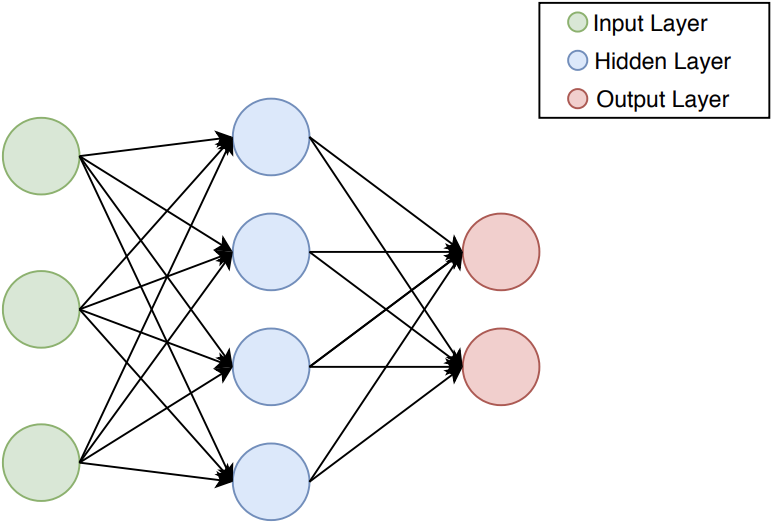
\includegraphics[scale=0.5]{images/implementation/neural_network_diagram.png}
	\caption{An example diagram of a Feedforwrd Neural Network with 1 hidden layer}
	\label{figure-neural_network_diagram}
\end{figure}		

\subsubsection{Notation and Network Representation}\label{imp_ffn_functions}

For the purposes of this chapter, the following notation will be used:

\begin{itemize}
\item[1] A network $N$ will be contructed with $L$ layers, each with $e$ nodes
\item[2] The weights from the $j^{th}$ node in the $l^{th}$ layer from the $k^{th}$ node in the $(l-1)^{th}$ layer are represented by $w^l_{jk}$
\item[3] The bias for the $j^{th}$ node in layer $l$ is represented by $w^l_0j$
\item[4] The output for the $j^{th}$ node is defined as $a = o(z_j)$, for an activation function $o$ (with inverse $o^{\prime}$) and weighted input $z$
\item[5] The weighted input for the $j^{th}$ neuron in a layer is 
\begin{equation}\label{eq_weighted_input}
	z^l_j=\sum_{i=1}^{e^{l-1}}{a^{l-1}_iw_{ij}} + w_{0j}
\end{equation}
\end{itemize}
~\\
These definitions allow an input into the network to be propagated through it, having the original values processed through the weights and activations functions, and have an output in the form of the network's last layer.

\subsubsection{Activation Functions}\label{imp_activation_functions}
~\\
As noted in \ref{lr_activationfunctions}, there are 3 primary characteristics of concern for activation functions: non-linearity, continuous differentiability and monotonicity. While many different functions have been suggested and used, several of the more popular were implemented here.

\subparagraph{Sigmoid}

The sigmoid, or logistic, function is one of the most popular and widely used activation functions historically, and is defined as 
\begin{equation}\label{func_sigmoid}
\texttt{o}(x) = \frac{1}{1 + e^{-x}}
\end{equation}

\begin{equation}\label{func_sigmoidprime}
\texttt{o}^\prime(x) = \texttt{o}(x)(1-\texttt{o}(x))
\end{equation}

The Sigmoid function is in the range [0,1], making it a suitable choice for problems requiring a probabilistic output. The slope of the function curve is both a boon and a drawback: it allows for fast learning initially, but results in learning slowdown later (often casuing what is referred to as node 'saturation'). The exponent calculation is also computationally expensive, relatively speaking.

\subparagraph{ReLU}

The Rectified Linuear Unit (ReLU) is a newer activation function which has been shown to be effective in deep learning networks. It is defined as

\begin{equation}\label{func_relu}
\texttt{o}(x) = \texttt{max}(0, x)
\end{equation}

\begin{equation}\end{equation}\label{func_relu_prime}
\[
\texttt{o}^\prime(x)= 
\begin{cases}
1,& \text{if } x\geq 0\\
0,              & \text{otherwise}
\end{cases}
\]

The function has the benefits of quick learning which doesn't saturate, as well as being computationally cheap. The downside is that the non-gradient for the negative range of the function can result in 'dead' nodes, which stop updating with the learning process.

\subparagraph{Leaky ReLU}

The Leaky ReLU resolves the dying ReLU problem by adding a small gradient to the negative range of the function. This results in a slow learning being applied to 'dead' ReLU's, which may in turn result in them being used again if necessary.
\begin{equation}\end{equation}\label{func_leaky_relu}
\[
\texttt{o}(x)= 
\begin{cases}
x,& \text{if } x\geq 0\\
0.01x,              & \text{otherwise}
\end{cases}
\]

\begin{equation}\end{equation}\label{func_leaky_relu_prime}
\[
\texttt{o}^\prime(x)= 
\begin{cases}
1,& \text{if } x\geq 0\\
0.01,              & \text{otherwise}
\end{cases}
\]

\subparagraph{Linear Activation}

Linear activations don't transform the input, and have a constant gradient, which can be useful for key layers where no loss in error signal is desired, such as the output or encoding layers.

\begin{equation}\label{func_linear}
\texttt{o}(x) = x
\end{equation}

\begin{equation}\label{func_linear_prime}
\texttt{o}^\prime(x) = 1
\end{equation}

\subsubsection{Backpropagation}\label{imp_backprop}

The backpropagation algorithm, as discussed in \ref{lr_trainingbackprop}, has allowed for effective training of FNNs for given data. The algorithm relies on incremental improvements of the model, as defined by decreasing the cost function. A common choice for cost is Mean Squared Errors (MSE):

\begin{equation}\label{func_MSE}
C = \frac{1}{2} \rVert y - a^L \rVert^2
\end{equation}
~\\

A technical definition of the backpropagation algrithm is given in Algorithm \ref{algo_backprop}, though the three primary steps of the algorithm are:\newline
\begin{itemize}
	\item [1] \textbf{Forward Pass}: The samples are propagated through the network, in order to generate the output $\hat{y}_s$. Vectorization is typically used to calculate the results for multiple samples at once, though conceptually each sample is used as input for the first layer, and subsequent layers use the weighted output from the previous layer passed through the activation function as input, using equation \eqref{eq_weighted_input} for the weighted output and the equations defined in \ref{imp_activation_functions} for the activation functions.
	\newline
	\item [2] \textbf{Calculate Cost}: The cost between the training output $y_s$ and the model output $\hat{y}_s$ is calculated. Using this cost function, the rate of change for the error in the output layer by the rate of change in the activation function in the last layer. This is captured in equation \eqref{eq_lambda1}:	
		\begin{equation}\label{eq_lambda1}
		\delta_{j}^{L}=\frac{\partial C}{\partial a_{j}^{L}} o^{\prime}\left(z_{j}^{L}\right)
		\end{equation}
	The vectorized version of this is often used, and expressed in \eqref{eq_lambda2}, where $\nabla_a C$ represents a vector of components which represent the partial derivatieves, such that they represent the rate of change of C relative to the activation functions' outputs.
		\begin{equation}\label{eq_lambda2}
		\delta_{j}^{L}=\nabla_a C \otimes o^{\prime}(z^L)
		\end{equation}
	If using quadractive cost, as per \ref{func_MSE}, then the term $\frac{\partial C}{\partial a_{j}^{L}}$ can be reduced to $(a^L - y)$, such that the equation for the output layer error is
	\begin{equation}\label{eq_lambda3}
				\lambda^L = (a^L - y) \otimes o^{\prime}(z^L)
	\end{equation}
	\newline		
	\item [3] \textbf{Backwards Pass}: The backwards pass consists of 2 steps, where the errors for each previous layer are calculated, and the weights for that layers are then adjusted accordingly:
		\begin{itemize}
		\item [3.1] The activation values are propagated back through the network to calculate the delta values based on the cost value. This uses the same rationale as \eqref{eq_lambda1}, but rather uses $(w^{l+1})^T$ by the next layers error in order to get an indication of how the error rate and how it moves backwards through the network.
						\begin{equation}\label{eq_lambda4}
						\lambda^l = ((w^{l+1})^T\lambda^{l+1})  \otimes o^{\prime}(z^l)
						\end{equation}
		\item [3.2] In order to update the network, each weights output error and input activation are multiplied to find the weight’s gradient and this gradient is reduced by a factor of the ‘learning rate’ $\eta$, which is then subtracted from the network weights to update them proportionately to the error observed and chosen learning rate.
						\begin{equation}\label{eq_bp_weightupdate}
						w^l \rightarrow w^l - {\eta}\lambda^{l} (a^{l - 1})^T
						\end{equation}
	\end{itemize}
		
\end{itemize}

Choices regarding the learning rates are discussed in \ref{imp_learning_rate_schedule} and the full algorithm is presented below in Algorithm \ref{algo_backprop}.\newline

\RestyleAlgo{algoruled}
\begin{algorithm}[H]
	\KwIn{Neural Network $N$, with randomly initialized weights $w$, $L$ layers, and activation functions $o$ and learning rate $\eta$}
	\KwData{Testing set with inputs $x$, and outputs $y$}
	
	\texttt{\\}

	\Repeat{no new samples can be drawn from $x$}{
			Select a sample $x_s$ from $x$\;
		
			\tcp{Perform the Forward Pass,  to calculate the network output, $y_s$, for input sample $x_s$}
			$a_0$ =  $x_s$;
			\texttt{\\}
			\ForEach{l in 1:L}
			{
				\ForEach{j in 1:$e^l$}
				{
					$z^{l}_j=\sum_{i=1}^{e^{l-1}}{a^{{l-1}}_iw_{ij}} + w_{0j}$;
					\newline
					$a^{l}_j$ = $o(z^{l}_j)$;
				}
			} 
			\tcp{Calculate the error term (aka cost), as}
			$\lambda^L = (a^L - y) \otimes o'(z^L)$;
			
			\texttt{\\}
			\tcp{Perform the Backward Pass, to propagate the errors back and update the network accordingly}
			\ForEach{l in (L-1):1}
			{
				\tcp{Calculate the delta values}
				$\lambda^l = ((w^{l+1})^T\lambda^{l+1})  \otimes o'(z^l)$;
				
				\tcp{Update the weights}
				$w^l \rightarrow w^l - {\eta}\lambda^{l} (a^{l - 1})^T$;
			}
	}

	\KwResult{Updated Network $N$}
	\label{algo_backprop}
	\caption{Backpropagation}
\end{algorithm}




\subsubsection{Gradient Descent Algorithms}\label{imp_sgd}

The backpropagation algorithm is defined at a single sample level, and the learning from a dataset is usually repeated for a number of 'epochs'. As noted though, implementation is often implemented using a vectorized version of the algorithm which either samples the entire dataset at once (batch), or a subset of samples (minibatch). The latter is the Stochastic Gradient Descent (SGD), as discussed in \ref{lr_OGD}, which has been shown to increase the speed and stability at which the backpropagation algorithm can converge to a minima in terms of cost. The algorithm runs backpropagation over the entire dataset for the number of epochs, and updates the network incrementally through the epoch. The stopping condition for the algorithm is usually defined as either a particular number of epochs being reached, or cost no longer decreasing for some number of epochs (i.e. a minima has been reached).\newline

The changes to the initial backprop algorithm, detailed in \ref{algo_backprop}, are relatively minor:
\begin{itemize}
	\item [1] Selection is now performed such that at each epoch $m$ samples $x_s$ are selected from $x$ which have not yet been sampled.
	\item [2] The weight update is now performed such that it represents an aggregate update according the $m$ samples that were selected:
			\begin{equation}\label{eq_backprop_weightupdate_sgd}
			w^l \rightarrow w^l - \frac{\eta}{m} \sum_{x} \lambda^{x, l} (a^{x, l - 1})^T
			\end{equation}
\end{itemize}

\texttt{}\newline 

\subparagraph{Online Gradient Descent}
Where SGD is appropriate and effective for scenarios where the entire dataset is available, Online Gradient Descent (OGD) is applicable for when the model is learning in an online fashion. In this case, the backpropagation is run as defined above in Algorithm \ref{algo_backprop} but with no repetition (i.e. only 1 epoch).

\subsubsection{Regularization}\label{imp_regularization}

Regularization is a commonly used technique in machine learning used to reduce a model's capacity to overfit to the data, and in so doing reduces the variance in the model results. One of the typical methods, $L2$ (or "weight decay"), is implemented by adding an extra term to the cost function which is itself a function of the weights in the model. This extra term forces the learning process to favour smaller weights, and only allows large weights to occur if they are able to offer an appropriate increase in performance. The modified cost function is displayed below in \ref{func_l2reg}.

\begin{equation}\label{func_l2reg}
C=\frac{1}{2 n} \sum_{x}\left\|y-a^{L}\right\|^{2}+\frac{\lambda}{2 n} \sum_{w} w^{2}
\end{equation}

The additional term is scaled by the configurable regularization parameter, $\lambda$, which if small approximates the original cost function or if large will increase the degree of regularization used. \newline

In order to implement this in backpropagation, the weight update rule is changed to the following (while biases remain the same):

\begin{equation}\label{func_l2_weight_update}
w \rightarrow w-\eta \frac{\partial C_{0}}{\partial w}-\frac{\eta \lambda}{n} w
\end{equation}

For SGD, this can be simplified to the following: 

\begin{equation}\label{func_sgd_l2}
w \rightarrow\left(1-\frac{\eta \lambda}{n}\right) w-\frac{\eta}{m} \sum_{x} \frac{\partial C_{x}}{\partial w}
\end{equation}


\subsubsection{Learning Rate Schedule}\label{imp_learning_rate_schedule}

Learning rates schedules are implemented to allow for a more dynamic exploration of the possible solution space, and allow fine tuning around an optima. With a constant learning rate implementation, one has to choose between a larger learning rate which allows faster progress but less optimisation, or a smaller learning rate which learns slower but is more effective at optimising (by avoiding the learning algorithm from bouncing around a minima valley). Learning rate schedules aim to get the best of both scenarios by cycling through a minimum and maximum range across epochs.\newline

The learning rate schedule is specified to cycle through from min to max every $i$ epochs, from $\eta_{\min}$ to $\eta_{\max}$. Thus for the current epoch $T$, the learning rate is calculated using \ref{func_learning_rate_sched} below:

\begin{equation}\label{func_learning_rate_sched}
\eta_{t}=\eta_{\min }^{i}+\frac{1}{2}\left(\eta_{\max }^{i}-\eta_{\min }^{i}\right)\left(1+\cos \left(\frac{T_{\text {current}}}{T_{i}} \pi\right)\right)
\end{equation}

This is the Cyclical Learning Rates approach, though using sinusoidal form rather than linear \cite{Smith}. For a minimum learning rate of 0.1, a maximum of 1.0 and an epoch cycle of 100, it will produce learning rates as displayed in figure \ref{figure-SGDRLearningRates} below.

\begin{figure}[H]
	\centering
	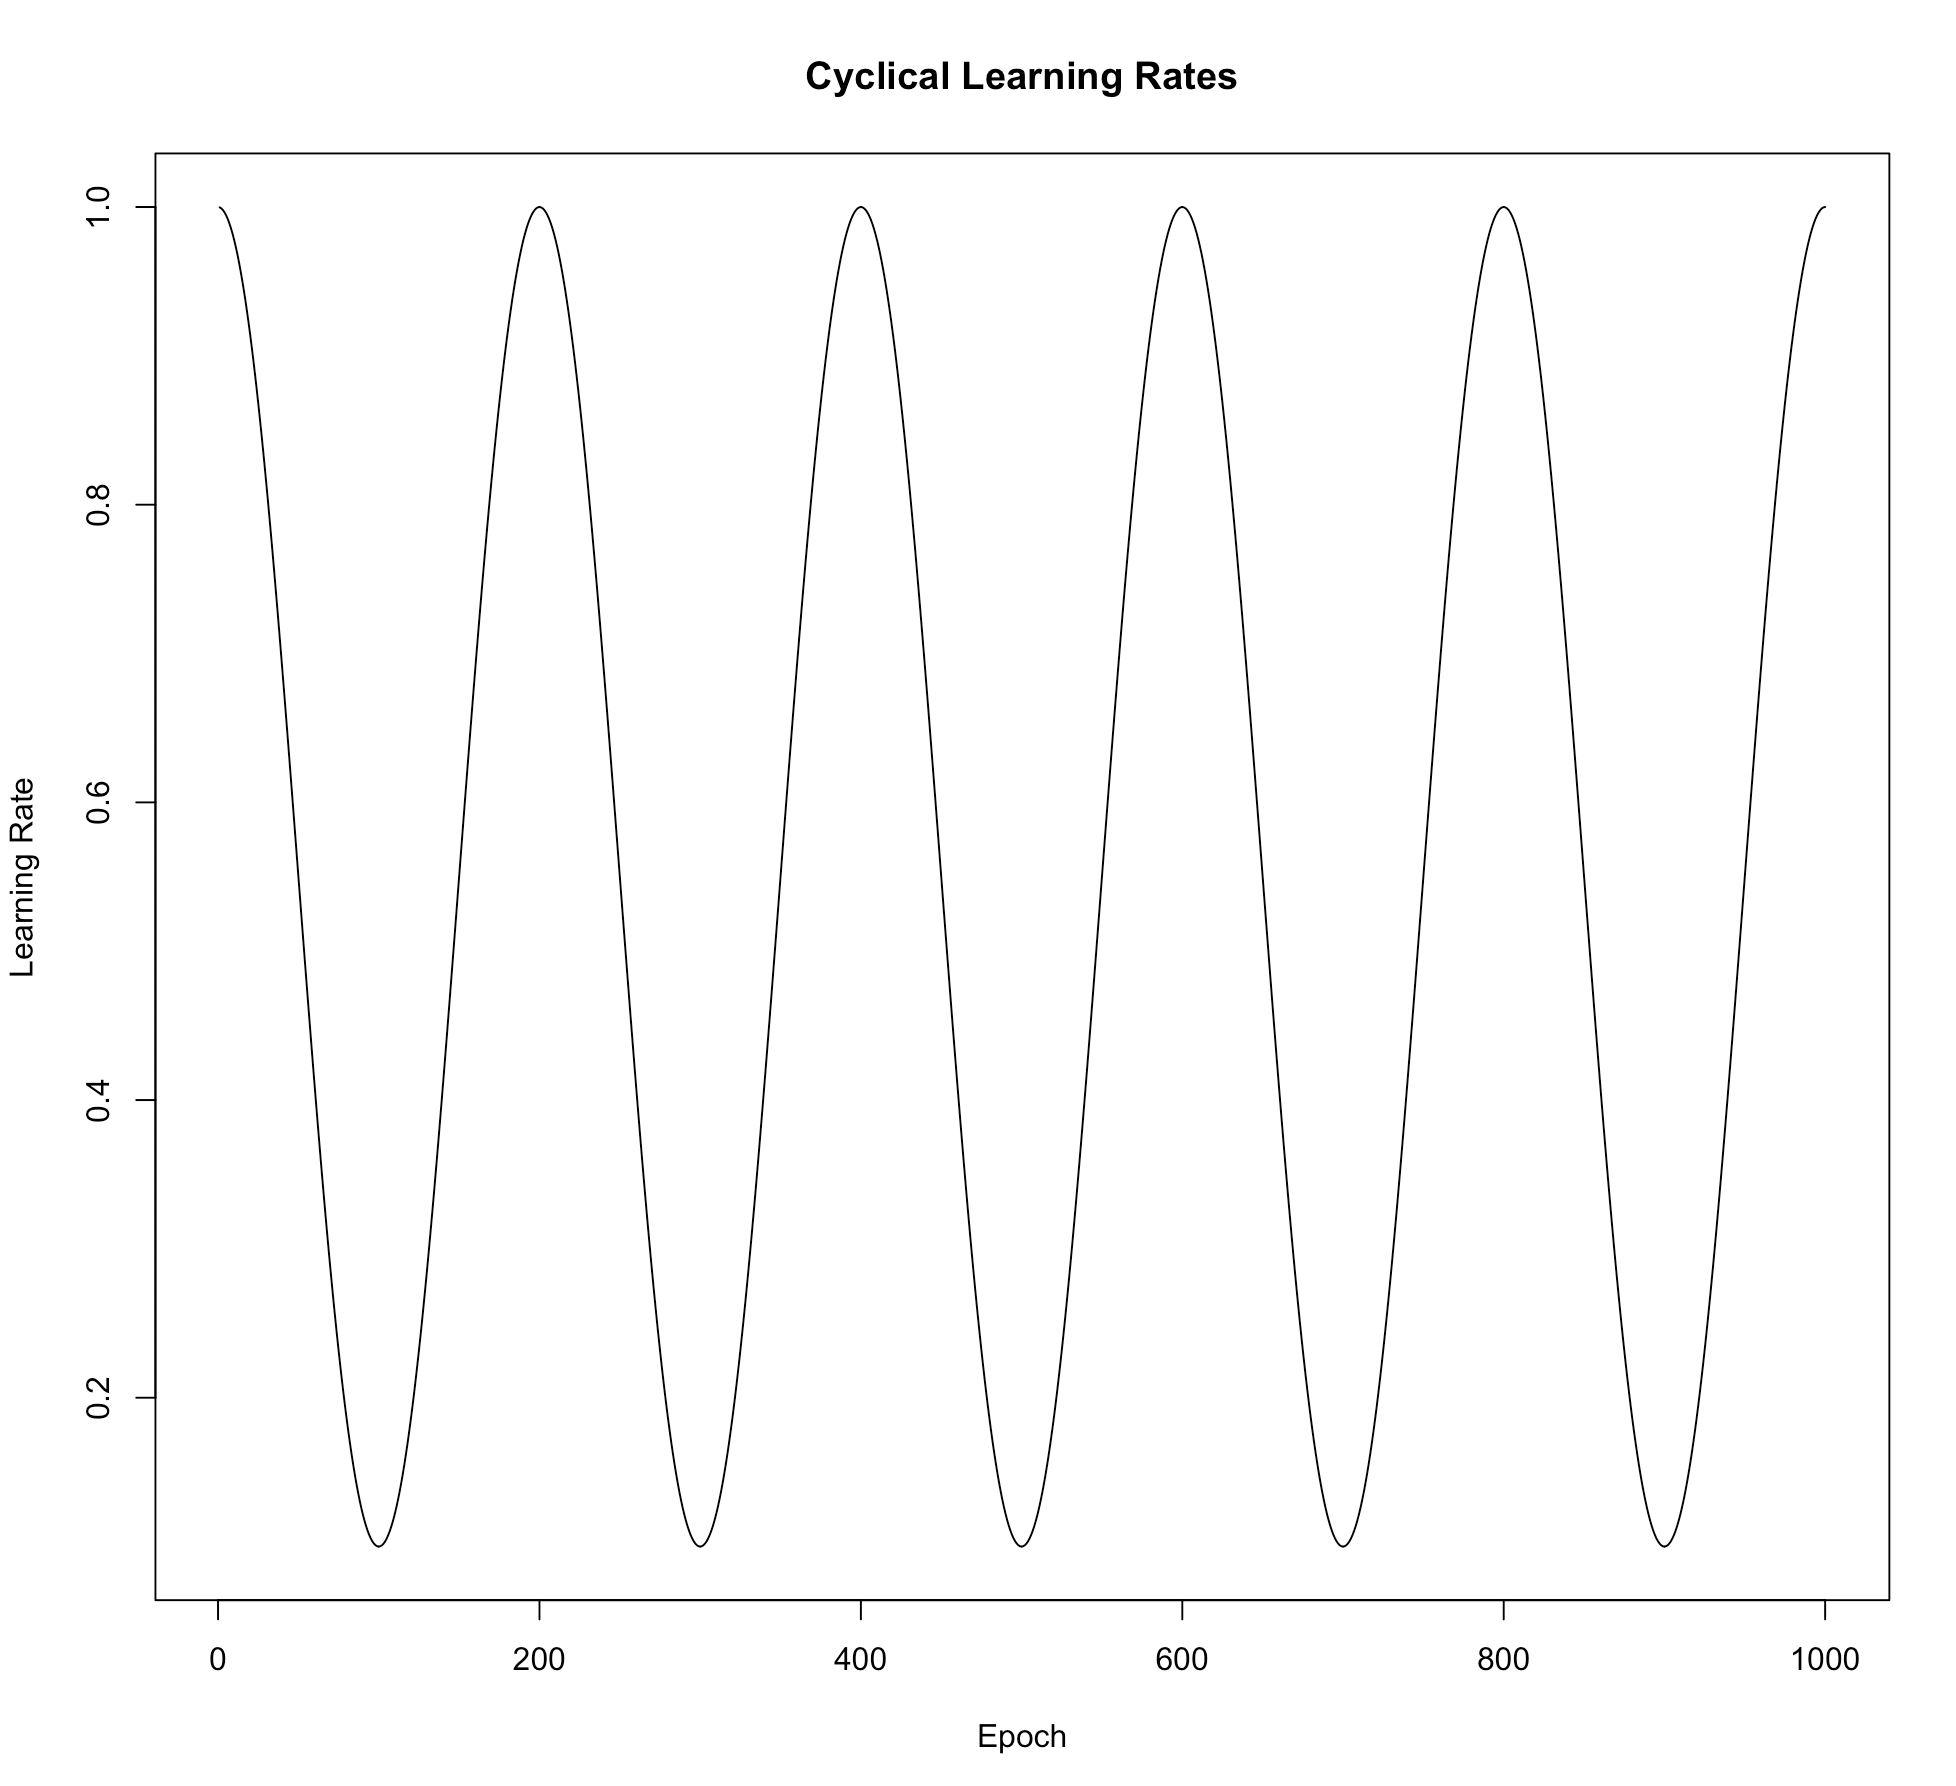
\includegraphics[scale=0.2]{images/implementation/CyclicalLearningRates.png}
	\caption{Learning rates calculated over 1000 epochs with $\eta_{\min} = 0.1$ to $\eta_{\max} = 1.0$ and $i=100$}
	\label{figure-SGDRLearningRates}
\end{figure}

\subsubsection{Dropout}

Input layer dropout has been implemented in order to perform regularization on the data features. The methodology used will set a percentage of the features for each sample to 0 during the SGD training process. While the percentage stays the same throughout the testing process, the features selected for each sample are rechosen every time it is used (i.e. for subsequent epochs). Conceptually, the dropout as applied to the input layer may result in the network learning relations between assets and possible patterns that would improve predictive efficacy.

\subsection{Restricted Boltzmann Machines}\label{imp_rbm}

Restricted Boltzmann Machines (RBM) are generative networks which can be trained to learn probability distributions over a dataset. They are structurally different from a FFN in that they have a recurrent weight function - a typical RBM has one visible layer (input/output), and one hidden layer. A sample will be processed from the input layer to the hidden layer, and the activation values from the hidden layer will be used by the input layer to provide a recontruction. The hidden units thus correspond to feature detection of the visible unit data structures, and the learning process of the network results in effective parameter estimation. \newline

\begin{figure}[H]
	\centering 
	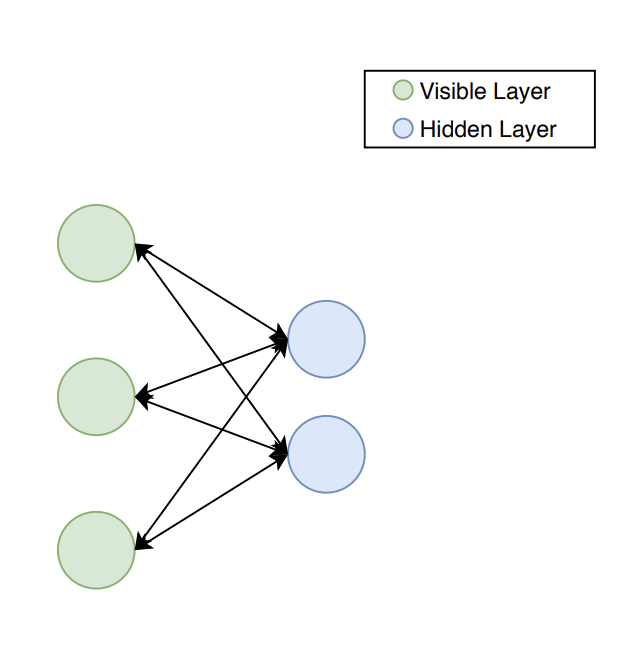
\includegraphics[scale=0.5]{images/implementation/rbm_network_diagram.png}
	\caption{An example diagram of a Restricted Boltzmann Machine network}
	\label{figure-rbm_network_diagram}
\end{figure}		

One of the primary differences from a FFN lies in the stochastic unit determination - the values in a hidden layer will typically be implemented such that the take on a binary value with a probablistic likelihood. Thus, the input and output have the same structure, and the processing from the hidden layer creates the generative process learned by the RBM. \newline

The joint configuration $(v,h)$ of the visible and hidden units has an energy given by:

\begin{equation}\label{func_rbmenergy}
E(v,h) = - \sum_{i \in visible} a_iv_i - \sum_{j \in hidden} b_jh_j - \sum_{i,j}v_ih_jw_ij
\end{equation}

where $v,h$ correspond to the binary states of the visible and hidden units, with biases $a,b$, and weights $w$ \cite{Hinton5}. It can be shown, that network weights can be adjusted to change the probabilities assigned to a particular training sample \cite{Hinton5}. The derivations of \ref{func_rbmenergy} show that performing a stochastic descent for the log probability of the data can be implemented through the following weight adjustment:

\begin{equation}
\Delta w_{ij} = \eta (\langle v_ih_j\rangle_{data} - \langle v_ih_j\rangle_{model})
\end{equation}

The angular brackets here indicate expectations under the distribution specified by the following subscript. Due to the probabilistic nature of RBMs, the [0,1] ranged Sigmoid activation function is typically used. Thus, for hidden nodes and a data sample $v$, it is easy to get unbiased sampling of $\langle v_ih_j \rangle_{data}$

\begin{equation}
p(h_j=1) = \sigma(w_{0j} +  \sum_{i=1}v_iw_{ij})
\end{equation}

Similarly, the visible states (or reconstruction), can then be calculated as 

\begin{equation}
p(v_i=1) = \sigma(w_{0i} + \sum_{j=1}h_jw_{ij})
\end{equation}


Getting an unbiased sample of $\langle v_i h_j \rangle$ proves more problematic, and so the model reconstructions via Gibbs sampling are used instead (this is explained below), resulting in the weight updates of

\begin{equation}
\Delta w_{ij} = \eta (\langle v_ih_j\rangle_{data} - \langle v_ih_j\rangle_{reconstruction})
\end{equation}

While it's important for the hidden units to take on a binary value (and so avoid communicating real values rather than learning structure), the visible units may be chosen to take on the probability values, rather than the stochastic samples, particularly if real valued output is necessary. 

\subsubsection{Contrastive Divergence}\label{imp_CD}

The process of sampling and resampling may be run for many iterations between the two layers before finishing on an output - this potentially long running and stochastic process results in the generative aspect of the network, and constitutes a Gibbs sampling chain. Multiple sampling steps in this chain is known as Contrastive Divergence, or CD-n, where $n$ represents the number of steps, and which allows for effective parameter estimation. Thus, CD-1 is the following:\newline


\begin{algorithm}[H]
	\KwIn{RBM Network $N$, with visible nodes $N$ and hidden nodes $H$ and distribution $\langle vh \rangle$}
	\KwData{Training sample dataset $V'$}
	
	\texttt{}\newline
	
	For a random training sample $V'$, sample $H'$ from $P(V|H)$;\newline
	Sample $V$ from $P(V|H')$;\newline
	Sample H from $P(H|V)$;\newline
	Return $(V,H) \sim R $, where R is the reconstructed distribution for $\langle vh \rangle$;\newline
	
	\tcp{Using the reconstructed distribution $R(V,H)$, the weight update for CD-1 is, as above, then}
	 
	\begin{equation}
	\Delta CD(W) = \eta( E_{P(H|V)D(V)}[VH^T] - E_{R(V,H)}[VH^T])
	\end{equation}
	
	
	\KwResult{Reconstructed distribution for $\langle vh \rangle$}
	
	\label{algo_cd1}
	\caption{CD-1}
\end{algorithm}

There's no upper bound on the iterations used for CD, and running for many can prove more effective for certain purposes. In this case however, where RBMs are used for the purposes of weight initialization, CD-1 is usually deemed sufficient.

\subsubsection{CD-1 and SGD}

In the same way that the backpropagation learning algorithm in \ref{imp_backprop} can be implemented in an SGD process for FFNs, so can the CD learning algorithm for RBMs. The framework is kept the same, with the implementation of epochs and weight updates based on stochastically chosen minibatches, but the calculation used to update the weights is CD-1 instead.


\subsection{Stacked Autoencoders}\label{imp_SAE}

As noted in \ref{lr_SAE}, the use of Stacked Autoencoders (SAE) have resulted in significant improvements in deep learning networks, and allowed effective reduction of high dimensional data. A single layer autoencoder is a specialized type of FNN with 3 layers: one input, one hidden, and one output. The network is trained (using backpropagation as per \ref{imp_backprop}) to reconstruct the input, so the input and output layers have the same structure, and the hidden layer needs to have fewer nodes than the input. This forces the hidden layer to learn effective features of the data, and reduce the dimensional representation. 
\newline\newline
Stacked autoencoders follow a similar structure, but with multiple hidden layers. The only strict requirement of the hidden layers is that the middle one, which will be used as the encoder layer, still has fewer nodes than the input. This structure can still be trained using backpropagation, but with more layers, it is likely to begin suffering from the vanishing or exploding gradient problem. As noted, the work by Hinton et al. for initialization of weights helps resolve this.

\subsubsection{Sigmoid based Greedy Layerwise SAE Training}\label{imp_sigmoidsae}

The steps for implementing the SAE training suggested by Hinton et al \cite{Hinton2} is as follows

\begin{itemize}
	\item [1] Define a network structure which conforms to the requirements of an SAE, with $L$ layers
	\item [2] For the first hidden layer, train as you would for an RBM with 2 layers - with the input layer, and the first layer as the hidden layer, using CD-1 and SGD
	\item [3] For each layer $l$ in $(2, L/2)$:
	\begin{itemize}
		\item [3.1] Process the data through the previously trained layers using the forward propagation as defined in \ref{imp_ffn_functions}
		\item [3.2] This processed data then forms the input to the $l^{th}$ layer, which can be trained once again using CD-1 and SGD as if it were two layers
	\end{itemize}
	\item[4] Once all the layers up until the encoder layer have been trained in this greedy layerwise fashion, mirror the weights and layers structures after the encoder to create a fully $L$ layered FFN with pre-trained weights
	\item [5] This network can then be trained using the backpropagation and SGD algorithms, where cost of reproducing the network input is minimised
	\item [6] Once a minima or acceptable level of reconstruction has been reached, the network can be truncated as the encoder layer, and so the first $L/2$ layers are used as the SAE
\end{itemize}

Notably, this weight initialization will only be effective if the RBM and SAE networks use the same activation function, which due to the RBM implementation, needs to be a function that can output a probabilistic value in [0,1].

\subsubsection{ReLU based SAE Training}\label{imp_relusae}

ReLU activations differ from Sigmoid in that they are not fitting for probability estimations, which makes the algorithm suggest by Hinton et al. unsuitable. The process used here relies on effective weight initialization, and is a simplification of the above.

\begin{itemize}
	\item [1] Define a network structure which conforms to the requirements of an SAE, with $L$ layers
	\item [2] Use an effective weight initialization, such as Xavier or He (discussed fully in \ref{imp_weights})
	\item [3] This network can then be trained using the backpropagation and SGD algorithms, where cost of reproducing the network input is minimised
	\item [4] Once a minima or acceptable level of reconstruction has been reached, the network can be truncated as the encoder layer, and so the first $L/2$ layers are used as the SAE
\end{itemize}

\subsubsection{Denoising Autoencoders}

As noted in \ref{lr_SDAE}, denoising can be used as an optimization technique for autoencoders in order to improve general performance and reconstruction. The methodology works by corrupting the input data for training, but using the non-corrupted data as the expected output sample. In doing so, this forces the autoencoder to learn more fundamental representations of the data rather then fitting to sample noise, hence "denoising". Two of the more typical techniques for achieving this have been implemented, as detailed below. In both cases, the noise is reapplied each time training samples are chosen.

\subparagraph{Additive Gaussian Noise}

With Gaussian noise, samples are corrupted such that a degree of variance is added to the input according to a parameterized Gaussian distribution. In this case, the distribution variance is a configurable training parameter.

\begin{equation}
\tilde{{x}} | {x} \sim \mathcal{N}\left({x}, \sigma^{2} I\right)
\end{equation}

\subparagraph{Masking Noise}

With masking noise, a fraction of the features in the data are set to 0, thus masking them for that sample. The percentage of features chosen is a configurable training parameter.

\subsection{Variance Based Weight Initializations}\label{imp_weights}

Recent research, as noted in \cite{He}, has shown that weights can be initialized to maintain expected variance between the input and output layers. These methodologies have the immediate advantages of simpler implementation, as well as faster computation (as no pre-training is required). The also allow for effective weight initialization of non-probabilistic activation functions, such as ReLU. Whether they result in better reconstructions or predictions is less clear (especially as the linearity assumption would prove faulty), and so the methods are tested here as well. 
\newline\newline
A common initialization heuristic is to use a uniform, and but not layer agnostic, initialization such as \ref{func_uniform_init} below. While simple enough, it's been shown that this does not always lead to the best training results, and can be outperformed by variance based initializations \cite{Glorot}.

\begin{equation}\label{func_uniform_init}
\text{weights} \sim U\left[-\frac{1}{\sqrt{n}}, \frac{1}{\sqrt{n}}\right] \textit{ , for a layer with n nodes}
\end{equation}

\subsubsection{Initialization Rationale}

The variance balancing methodology is based on balancing the variance of a linear network. For input $X$, with $n$ components and linear neurons with weights $W$, and output $Y$,
\begin{equation}
Y = W_1X_1 + W_2X_2 + ... + X_nW_n
\end{equation}
It can thus be shown, that for $i.i.id$ samples with mean $0$, then
\begin{equation}
Var(Y) = nVar(W_i)Var(X_i)
\end{equation}
For the variance of both input $X$ and output $Y$ to be balanced on the forward and backward propagation, then it is necessary for
\begin{equation}
Var(W_i) = \frac{1}{n_{in}}= \frac{1}{n_{out}}
\end{equation}

In the instance where there are not an equal number of nodes in the two layers, the average can be taken, such that
 \begin{equation}\label{eq_init_var}
Var(W_i) = \frac{2}{n_{in} + n_{out}}
\end{equation}

\subsubsection{Initializations}

\subparagraph{Xavier} Considering that  $Var(U(-a, a)) = a^2/3$, then ensuring balance variance for weights as per equation \eqref{eq_init_var} provides us with the Xavier Glorot initialization \cite{Glorot} which can be used for Sigmoid activations, and is defined as follows
\begin{equation}
w_{ij} \sim U(-r, r), r = \sqrt{\frac{6}{n_i + n_j}}
\end{equation}

where $n$ is the number of nodes in the $i^{th}$ or $j^{th}$ layer.
\newline\newline
\subparagraph{He} The initialization for ReLU is different on accounts of the function being equal to zero for half it's potential input range - in this case it makes sense to double the weight variance, and so the He \cite{He} initialization is used

\begin{equation}
w_{ij} \sim U(-r, r), r = \sqrt{\frac{6}{n_i}}
\end{equation}


\subparagraph{He-Adjusted} An adjusted initialization is presented here, dubbed 'He-Adjusted', where the ReLU initialization uses a mean of the input and output layers in order to scale the weight variance. For networks with constant layer sizes, the intialization is the same as He, though for SAE networks which have layer size changes by definition, the He-Adjusted initialization will result in more appropriately sized weights.

\begin{equation}
w_{ij} \sim U(-r, r), r = \sqrt{\frac{6}{(n_i + n_j)/2}}
\end{equation}














\subsection{CSCV \& PBO}\label{imp_cscv}

The  combinatorially symmetric cross-validation (CSCV) method developed by Baily et al., as discussed in \ref{lr_cscv}, can be used to assess the likelihood of backtest overfitting through comparison of IS and OOS return metrics. Formulaically, the definition of backtest overfitting is given by
\begin{equation}\label{eq:PBO1}
\sum_{n=1}^{N}E[\overline{r_n}|r\in 
\Omega_{n}^{*}]Prob[r\in\Omega_{n}^{*}]\leq{N/2}
\end{equation}

Where the search space {\textOmega} consists of the N ranked strategies, and their ranked IS performance \textit{r} and OOS performance
\textit{\={r}}. This allows the PBO, using the Bayesian formula, to be defined as 

\begin{equation}\label{eq:PBO2}
PBO = \sum_{n=1}^{N}Prob[\overline{r} < {N/2}|r\in\Omega_{n}^{*}]Prob[r\in\Omega_{n}^{*}]
\end{equation}

Notably, the above definitions consider IS as the data made available to the strategy selection, rather than the 
models calibration (e.g. the full IS dataset, rather than, by was of example, the number of days used in a moving average). 
This allows the model-free and non-parametric nature of the definition. 
\hfill \break 

They further developed the CSCV framework as a methodology to reliably estimate the probability used in PBO, which allows a concrete application of the concept. The CSCV framework does not require using the typical ‘hold-out’ strategy (and thus avoids credibility issues), and is ultimately able to provide a bootstrapped distribution of OOS performance. The full methodology is shown in algorithm \ref{algo_cscv} below \cite{BailyPBO}.
\hfill \break 

\begin{algorithm}[H]
	\KwIn{$N$ configuration trials over $T$ time periods with P\&L}
	\texttt{\\}
		
	\begin{itemize}
			\item[1]Generate a TxN performance series matrix, $M$, representing the profits and losses by the $N$ configuration trials over $T$ time periods
			\item[2]Partition the $M$ matrix by rows into $S$ submatrices, each of even size ($T/S * N$)
			\item[3]Generate the combinations $C_S$ of $M_S$, in groups of size $S/2$, for total $\binom{S}{S/2}$ of combinations
			\item[4]For each combination in $c \in C_S$:
			\begin{itemize}
				\item [a] Form a training set $J$ by joinined $S/2$ $M_S$ submatrices, in their original order. $J$ is a matrix of order $(T/S)(S/2)*N $
				\item [b] Form the test set $\bar{J}$ as the complement of $J$ in $M$, once again in the original order
				\item [c] Form a vector of $R^c$ of performance statistics of order $N$, where the $N$th component $R_n^c$ of $R^c$ reports the performance associated with the $n^{th}$ column of $J$
				\item [d] Repeat [c] for $\bar{J}$ to derive $\bar{R}^c$ and $\bar{r}^c$
				\item [e] Determine the element $n^*$ such that $R^c_n \in \Omega^*_n$ - i.e. $n^*$ is the best performing strategy IS
				\item [f] Define the relative rank of $\bar{r}^c_{n^*}$ by $\bar{\omega}_c := \bar{r}^c_{n^*} / (N +1) \in (0,1)$. This is the relative rank of the OOS performance associated with the strategy chosen IS, which should systematically outperform OOS if no backtest overfitting has taken place
				\item[g] Define the logit $\lambda_c = ln \frac{\bar{\omega}_c}{(1-\bar{\omega}_c)}$. High values here indicate consistency between IS and OOS performances (and so low ovefitting)
			\end{itemize}
			\item [5] The logit values can now be used to compute the distribution ranks of OOS, by collecting all $\lambda_c$ for $c \in C_S$. The relative frequency for $\lambda$ occurring across all $C_S$ is 
			\begin{equation}
			f(\lambda) = \sum_{c \in C_S}\frac{\chi_{\lambda}(\lambda_c)}{\#(C_S)}
			\end{equation}
			where $\chi$ is the characterization function and $\#(C_S)$ is the number of elements in $C_S$, and so $\int_{-\infty}^{\infty} f (\lambda) d \lambda = 1$
		\end{itemize}
	
	\KwResult{Reconstructed distribution for $\langle vh \rangle$}
	\label{algo_cscv}
	\caption{CSCV}
\end{algorithm}



\texttt{\\}
\newline The CSCV framework and results thus allows the consideration of several notable statistics. First and foremost, 
the PBO may now be estimated using the CSCV method and using an integral over the $f(\lambda)$ function 
as defined above which offers a rate at which the best IS strategies underperform the median of OOS trials. The PBO is estimated using
\begin{equation}
\Phi = \int_{-\infty}^{0} f (\lambda) d \lambda
\end{equation}


If $\Phi \approx 0$,
it is evidence of no significant overfitting (inversely, $\Phi \approx 1$ would be a sign of probable overfitting). Critically then, a PBO measure may be used in a standard hypothesis test to determine if a model should be rejected or not. This 
can be extended, as shown by Bailey et al., to show the relationship between overfitting and performance 
degradation of a strategy. It becomes clear that with models overfitting to backtest data noise, there comes a point 
where seeking increased IS performance is detrimental to the goal of improving OOS performance.  
\hfill \break 


\subsection{Money Management Strategy and Returns}\label{imp_mms}

In line with the general approach here, the Money Management Strategy (MMS) has been designed to be relatively simple, such that the results are more indicative of the underlying modelling rather than intricate trading strategies. The MMS follows an arithmetic long strategy of buying any stock for which the predicted ${t+D}$ price is above the current price, and selling the stock at ${t+D}$. Trading costs have been included at 10\% capital costs per annum for borrowing to purchase, and 0.45\% for transaction costs. Results are compared to a "perfect" model which has exact knowledge of the price in $D$ days, which represents an upper bound on performance.
\hfill\break

\subparagraph{Input Variables}

The MMS takes the following values as input for each time point $t$  and prediction point $D$
\begin{itemize}
	\item [1] {$\texttt{y}_t$}, the closing price for $t$
	\item [2] $\texttt{y}_{t+D}$, the closing price in $D$ days
	\item [3] $\hat{\texttt{y}}_{t+D}$, the predicted closing price in $D$ days
\end{itemize}

\subparagraph{Calculated Stock Variables}

Using these, the MMS calculates and uses the following:

\begin{itemize}
	\item [1] A flag indicating whether a trade will take place on $t$
				\begin{equation}
				\texttt{trade\_long}_t = bool(\hat{y}_{t+5} > y_t) \in (0, 1)
				\end{equation}
	\item [2] A flag indicating whether a trade will take place on $t$ in the perfect model
				\begin{equation}
				\texttt{trade\_long}_{p,t} = bool({y}_{t+5} > y_t) \in (0, 1)
				\end{equation}
	\item [3] The observed return at $t+D$
				\begin{equation}
				\texttt{r}_{o, t + D} = y_{t+D} * trade\_long_t
				\end{equation}	
	\item [4] The expected return at $t+D$
				\begin{equation}
				\texttt{r}_{e, t + D} = \hat{y}_{t+D} * trade\_long_t 
				\end{equation}
	\item [5] The perfect return at $t+D$
				\begin{equation}
				\texttt{r}_{p, t + D} = y_{t+D} * trade\_long_{p,t}
				\end{equation}
	\item [6] The cost incurred in buying the stock at time $t$
				\begin{equation}
				\texttt{cost}_t = y_t * trade\_long_t
				\end{equation}
	\item [7] The cost incurred in the perfect model at $t$
				\begin{equation}
				\texttt{cost}_{p,t} = y_t * trade\_long_{p,t}
				\end{equation}
	\item [8] The possible capital and transaction costs
				\begin{equation}
				\texttt{trading\_cost}= y_t * (0.1 / 365 * 2) + y_t * (0.45 / 100)
				\end{equation}
	\item [9] The full cost of trading the stock at $t$ in the predictive model
				\begin{equation}
				\texttt{fullcost}_t = (y_t + trading\_cost_t) * trade\_long_t
				\end{equation}	
	\item [10] The full cost of trading the stock at $t$ in the perfect model
				\begin{equation}
				\texttt{fullcost}_{p,t} = (y_t + trading\_cost_t) * trade\_long_{p, t}
				\end{equation}
\end{itemize}

\hfill\break

\subparagraph{Calculated Strategy Variables} The MMS  is then implemented using these calculated values which are aggregated at each time point $t$ for all stocks, $s$, as follows:

\begin{itemize}
	\item [1] The expected return for $t+D$ from all stocks traded at $t$
					\begin{equation}
					\texttt{R}_{e, {t+D}} = \sum_{s \in stocks} r_{s, e, {t+D}}
					\end{equation}
	\item [2] The observed return for $t+D$ from all stocks traded at $t$
					\begin{equation}
					\texttt{R}_{o, {t+D}} = \sum_{s \in stocks} r_{s, o, {t+D}}
					\end{equation}
	\item [3] The perfect return for $t+D$ from all stocks traded at $t$
					\begin{equation}
					\texttt{R}_{p, {t+D}} = \sum_{s \in stocks} r_{s, p, {t+D}}
					\end{equation}
	\item [4] The cost of all trades at $t$
					\begin{equation}
					\texttt{C}_t = \sum_{s \in stocks} cost_{s,t}
					\end{equation}
	\item [5] The cost of all trades at $t$ in the perfect model
					\begin{equation}
					\texttt{C}_{p,t} = \sum_{s \in stocks} cost_{s, p ,t}
					\end{equation}
	\item [6] The cost of all trades at $t$ including transaction costs
					\begin{equation}
					\texttt{FC}_t = \sum_{s \in stocks} fullcost_{s,t}
					\end{equation}
	\item [7] The cost of all trades at $t$, including transation costs, in the perfect model	
					\begin{equation}
					\texttt{FC}_{p,t} = \sum_{s \in stocks} fullcost_{s, p ,t}
					\end{equation}	
\end{itemize}
\hfill\break
The final model return is thus established as $\sum_t{R_t} / \sum_t{C_t} $, for any variations of observed, expected or perfect returns as well as base and full costs. These model returns are used to establish the performance of the different predictive models which were trained.\newline
\hfill\break
An additional consideration of the MMS is the daily rates generated by the strategy, which incorporate the costs of any trades incurred, as well as any returns seen at $t$, such that 
\begin{equation}
\texttt{dailyrate}_t = R_{t-D} - C_t
\end{equation}

\newpage
\section{Implementation: Process}\label{imp_proc}

Having covered the technical implementations in Chapters \ref{Data} and \ref{Implementation}, a higher level overview of the end to end experimental process can be detailed. The process here rests on two key principles: implementing a generalised version of a system which could offer exploration of more complex techniques, and ensuring an effective modularisation of steps such that the process can be reconfigured accordingly while maintaining its integrity. In doing so, a separable system is created which brings together data reduction, deep learning with pre-training/weight initialization, online learning and back test overfitting validation.

\subsection{Data Preparation}\label{proc_dataprep}

The fulldataset goes through several steps of pre-processing - these are covered in more detail in \ref{data_processing}, though the steps are included here:

	\begin{itemize}
	\item[1] The data is processed into day to day log fluctuations
	\item[2] At each time point, rolling historic fluctuation summations are calculated (e.g. the past 1, 7 and 30 days)
	\item[3] At each time point, rolling future fluctuation summations are calculated (e.g. the next 2 days)
	\item[4] The dataset is truncated to only include points with all aggregations or predictions available
	\item[5] The dataset undergoes scaling - the different functions are detailed in \ref{data_scaling}, though \texttt{limited normalize} was used for most of the results produced
\end{itemize}

\subsubsection{Data Window Aggregations} The time aggregations were chosen according to domain knowledge - it's expected that prices may move in daily, weekly, fortnightly, monthly and quarterly patterns as trading is actioned by day traders such as speculators to institutional investors such as mutual funds. Indeed, it can be shown that markets can be modelled such that they are hierarchical in space and time, with actors at different heirarchical levels within the market interacting under different causitive structures \cite{Wilcox}. The effect is such that price trends and patterns can be expected to exist in time at multiple levels, with price being set as an emergent property of these hierarchies. Taking this into account, variations of 1, 5, 10, 20 and 60 working days were considered throughout the configuration tests, in the following combinations:  
\begin{itemize}
	\item[1.] 1,5,20 
	\item[2.] 5,20,60
	\item[3.] 10,20,60
\end{itemize}

\subsubsection {Point Predictions} Various configurations were tested in terms of the historic summations used, while the fluctuation predictions were either of 2 or 5 days. These are detailed more extensively in \todo{add result reference}. It's worth noting that the prediction horizon is configurable, and in the case of implementing a more complex trading strategy, one would likely choose to predict multiple points across the horizon in order to to develop a distribution. In this case, the MMS was kept purposefully simple, and so didn't warrant the more intensive implementation. \newline

One point of concern, is that point predictions at 2 or 5 days in advance could open the process up to aliasing error, as it is unlikely to be predicting at the Nyquist frequency, and may end up fitting to the band ripple rather than the underlying signal. Conversely, 1 day predictions for closing price might offer a high degree of accuracy, but are not practical for trading due to market auction and bidding structures. The system implementation veered on the side of practicality in this case, and was configured for longer term predictions despite the risk of aliasing. While some of the configurations were run with 2 day predictions, it was seen that once costs were considered it was difficult for even the benchmark to produce desired P\&L figures and so a 5 day prediction was generally implemented in subsequent tests. \todo{add result references}



\subsubsection {Scaling} When testing the two limited scaling methodologies, standardization and normalization, it was found that the results for standardizing tended to be notably worse than normalization (discussed in \ref{results_linearity}). It's possible that outliers in price fluctuations and changing variance through time (which is not captured effectively through the limited variation) resulted in a less informative representation and worse performance of the FNN models which can be prone to error maximisation. As a result of this, the limited normalization process was used for most of the tests run. It's worth noting that an implementation which incorporates processing the data through the Error Function in order to reduce the impact of outliers would likely prove a worthwhile endevour, and could be easily swapped in due to the systems modularity.\newline


\subsection{Data Segregation}\label{proc_dataseg}

Once processed, the dataset is split into 2 portions: the first set is used for the SAE training, as well as the initial SGD training on the predictive FFN network; the second set is used only for the OGD training in order to generate returns from the predictive network. In this sense, the first set is used as what would typically be the historical training set, and the second is used as the testing/validation set (the use of Bailey's CSCV technique negates the need for a hold-out portion of the dataset \cite{BailyPBO}). For the sake of clarity, these two subsets of the dataset will be referred to as the 'Training' and 'Prediction' datasets. \newline

In this case, a simple split point of 60\%/40\% was chosen for the Training and Prediction sets respectively. In a more restrictive case, where there is less data to work with, it would be advised to consider a method such as MinBTL as developed by Bailey et al. \cite{BaileyBTL} and the expected number of configurations to be tested in order to decide an appropriate split point.

\subsection{SAE Training}\label{proc_sae}

The Training dataset is used to train the autoencoder network using either RBM pretraining or weight initialization algorithms and SGD training, as defined in \ref{imp_SAE}. The Training portion of the dataset, as noted in \ref{proc_dataseg}, is itself split up into a training and validation set for the SAE. The efficacy of the SAE on the validation set is required in order to determine which networks to choose for subsequent steps in the process. The full testing process here will rely on a generated set of best SAE networks at each encoding layer size, to be used for FFN training and prediction (chosen by a minimum MSE score). The benefit of the modularised system is emphasised here, as the SAE training will not suffer from limitations due to backtesting considerations: any amount of configurations or processes can be tested for feature extraction without concern. \newline

Once the SAE networks have been defined and chosen, they can be used to reprocess both the Training and Prediction datasets such that the input is encoded, and the output is as before. These encoded datasets can then be used for the following steps in the process. \newline

In a productionized system, where data is updated daily, there would be a set period after which the SAE network would be retrained to reflect more recent data. While the system detailed here aims to emulate as much, it wasn't necessary to incorporate this step with the static dataset. \newline

\subsection{Prediction Network Training}\label{proc_predictionnetwork}

Typically, the SAE and predictive network might be presented as one and the same, however in the process presented we are able to separate the two and optimise for feature extraction prior to training for predictions. Having done so, the datasets can have their input encoded, but retain the same output. The predictive network is then trained using the Training set, as detailed in \ref{imp_backprop}. There's no requirement to validate this part of the training, so the dataset is not split into subportions as it was for SAE training. \newline

Once the predictive network is trained, the OGD process is run through the encoded Prediction dataset in order to generate the predictions for the assets prices that the model produces - thus emulating what would have occured in a live environment. \newline

\subsection{Price Reconstruction}\label{proc_precerecon}

In the interest of more intepretable results for figures such as P\&L, the prices are fluctuations are re-scaled back to their original price fluctuation predictions using the reverse scaling detailed in \ref{data_reverse_scaling}. These prices are then recostructed using \ref{data_price_recon}, such that they represent a predicted future price of the asset which can then be used by the MMS. It's worth nothing that the price reconstruction applies the predicted fluctuation to the known original price, such that it would represent a system that is run daily, rather then a system that is making rolling predictions over a period of time.

\subsection{Money Management Strategy}\label{proc_mms}

The MMS, as described in \ref{imp_mms}, takes a proof of concept approach to the system being investigated. It is a simple long strategy with a set liquidation point, and no notable refinement. The naive approach is taken purposefully here, so as not to bias the perspective of the system as a whole by the effects of an impactful trading strategy. A more effective trading strategy would incorporate a shorting side as well, though ultimately this isn't necessary in order to obtain a necessary indication of efficacy for the system (and conceptually, a consistently losing long strategy would be of interest in any case).  \newline

It is important, in the interest of effective optimization and development, that the pattern recognition in the prediction portion of the system is not tightly coupled with making it profitable. With this in mind, the modularity of the system is continued, with a distinct separation between the prediction signal and the MMS implementation which relies only on the predicted prices of each stock for a time point. The comparisons for the MMS are made against a benchmark of the same MMS, but with perfect information. This allows an indication for how effective the prediction system is (and need be) in order to generate comparable returns. \newline \todo{Can we learn to beat best stock paper ? Paper}

An effective production trading strategy would be likely to include stop losses or pyramiding stop losses for effective P\&L optimization. An ideal implementation, and possible area for further work, would include an MMS strategy where the bands for this are defined using a machine learning technique (rather than being chosen from domain knowledge or heuristics).\newline


\subsection{CSCV \& PBO}\label{proc_cscv}

The CSCV and PBO parts of the system are the most straightforward, in the sense that they are mostly just an implementation of the algorithm detailed in \ref{imp_cscv}. The CSCV process uses the returns from the MMS, which in turn used the prices from the predictions network. Conceptually, the whole system comes into place here, as the results from the CSCV process are now indicative of not only backtest overfitting in the trading strategy, but also in the prediction network and without having to consider the impact of many configuration tests for feature extraction.

\subsection{Process Diagram}\label{proc_diagram}

The flow diagram below provides a graphical representation of this process from the raw market data up until the price prediction points (the MMS calculations and CSCV process are not included). The process may be repeated accordingly in terms of SAE structures that are desired for testing, such that the "Best SAE Network" is different for different encoding layer sizes, or data aggregations used (as was the case in many of the experiments which will be discussed in \ref{Results}).

\begin{figure}[H]
	\centering 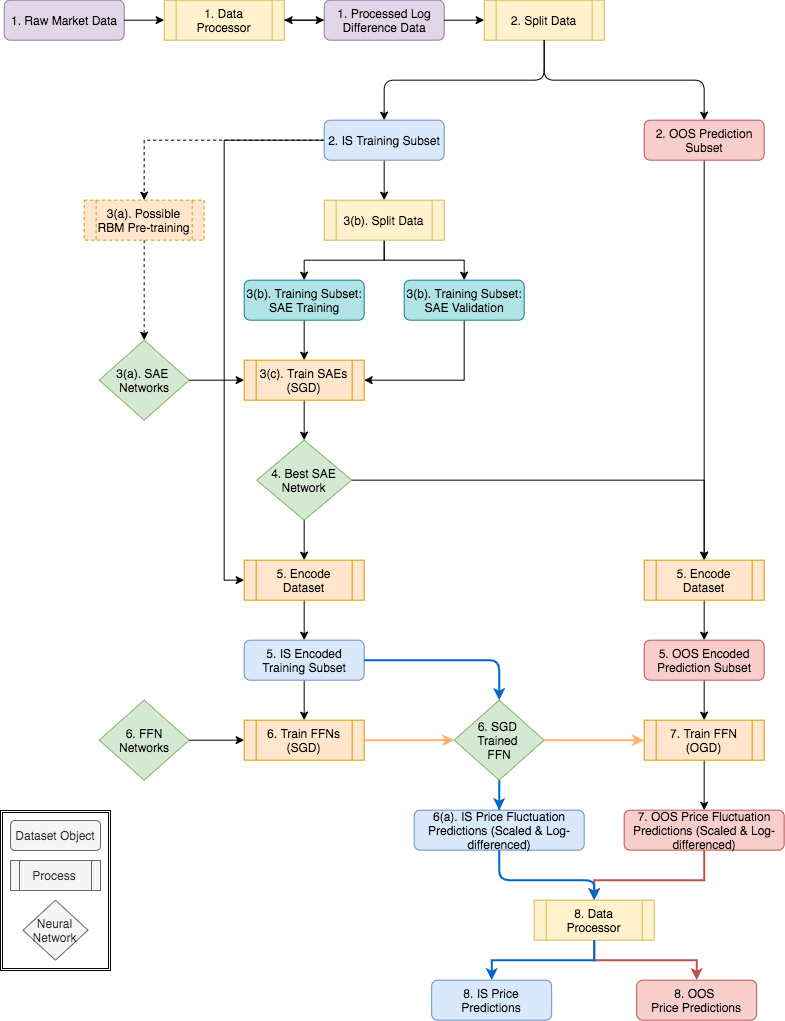
\includegraphics[scale=0.5]{images/process_implementation/process_flow.png}
	\caption{Overall Process Flow}
	\label{figure-proc_diagram}
\end{figure}






















\newpage
\section{Datasets Used}\label{Datasets}

\subsection{Synthetic Datasets}

Data was generated and scaled, as per the methods detail in \ref{data_synthetic} and \ref{data_scaling}. The sets were generated with the following configurations, each for 5000 timesteps and with a 60/40 split on the Training and Prediction sets.

\subsubsection{Synthetic6} \label{dataset_synthetic6}

The Synthetic6 dataset was configured to represent a combination of upwards, downwards and sideways Trends, each with high and low variance variations.

\begin{table}[h]
	\centering
	\begin{tabular}{|c|c|c|c|}
		\hline
		\textbf{Trend Category} &\textbf{Variance Category} & \textbf{Trend Mean} & \textbf{Variance}\\\hline	
		{Strong Upward} & {High} & {0.9} & {0.5} \\\hline
		{Strong Upward} & {Low} & {0.9} & {0.2} \\\hline
		{Upward} & {High} & {0.05} & {0.4} \\\hline
		{Upward} & {Low} & {0.05} & {0.1} \\\hline
		{Strong Downward} & {High} & {-0.8} & {0.55} \\\hline
		{Strong Downward} & {Low} & {-0.8} & {0.15} \\\hline
	\end{tabular}
	\newline\newline
	\caption{Synthetic 6 Dataset Configuration}\label{tab_synth6}
\end{table}

\subsubsection{Synthetic10}\label{dataset_synthetic10}

The Synthetic10 dataset was configured to represent a wide array of behaviours, including very high (positive and negative) mean stocks, as well as much lower mean stocks (which may be more representative of typical behaviour). These were chosen to make sure the network learning is able to differentiate and correctly learn across different asset categories.

\begin{table}[H]
	\centering
	\begin{tabular}{|c|c|c|c|}
		\hline
		\textbf{Trend Category} &\textbf{Variance Category} & \textbf{Trend Mean} & \textbf{Variance}\\\hline	
		{Strong Upward} 		& {High} & {0.9} & {0.5} \\\hline
		{Strong Upward} 		& {Low} & {0.7} & {0.2} \\\hline
		{Upward} 					& {High} & {0.05} & {0.5} \\\hline
		{Upward} 					& {High} & {0.05} & {0.4} \\\hline
		{Upward} 					& {Low} & {0.04} & {0.1} \\\hline
		{Sideways} 					& {Low} & {0.02} & {0.15} \\\hline
		{Sideways}					& {Low} & {0.01} & {0.05} \\\hline
		{Downwards}				& {Low} & {-0.1} & {0.2} \\\hline
		{Strong Downward} 	& {Low} & {-0.4} & {0.15} \\\hline
		{Strong Downward}	& {High} & {-0.8} & {0.55} \\\hline
	\end{tabular}
	\newline\newline
	\caption{Synthetic 10 Dataset Configuration}\label{tab_synth10}
\end{table}

\fcolorbox{red}{white}{This set was configured erroneously with the excessively high means.}

\subsection{Actual Datasets}

Several datasets have been used using JSE closing price relative data for 2003-2018 \todo{add ref}. They were processed the same way as the Synthetic sets, following the steps set out in \ref{Data} and with a 60/40 split on the Training/Prediction datasets.

\subsubsection{Actual10}\label{dataset_actual10}

This is the primary closing price dataset that has been used through out the experiment process, which focused on choosing more prominent stocks from multiple sectors.

\begin{table}[H]
	\centering
	\begin{tabular}{|c|c|c|}
		\hline
		\textbf{Code} &\textbf{Company} & \textbf{Sector} \\\hline	
		{AGL} & {Anglo American} & {Resources}  \\\hline
		{BIL} & {BHP Billigton} & {Resources}  \\\hline
		{IMP} & {Impala Platinum Holdings} & {Resources}  \\\hline
		{FSR} & {FirstRand Limited} & {Finance}  \\\hline
		{SBK} & {Standard Bank} & {Finance}  \\\hline
		{REM} & {Remgro Limited} & {Finance}  \\\hline
		{INP} & {Investec} & {Finance}  \\\hline
		{SNH} & {Steinhoff International Holdings} & {Retail}    \\\hline
		{MTN} & {MTN} & {Communication Services}  \\\hline
		{DDT} & {Dimension Data} & {Tech} \\\hline
	\end{tabular}
	\newline\newline
	\caption{Sytnetic 10 Dataset Configuration}\label{tab_actual10}
\end{table}


\subsubsection{AGL}\label{dataset_agl}

Using AGL data from JSE close price relatives.

\subsubsection{AGL\&ACL}\label{dataset_aglacl}

Using AGL and ACL data from JSE close price relatives.

\subsubsection{Scaling10}\label{dataset_scaling10}

Using the following assets from JSE close price relatives:

\begin{itemize}
	\item ACL, AGL, AMS, AOD, BAW, BIL, BVT, CFR, CRH, DDT
\end{itemize}











\newpage
\section{Results}\label{Results}


An introduction to the results, highlighting the important findings and sections. \todo{}


\subsection{Linearity, Complexity and Structure of Data}\label{results_linearity}

\subsubsection{GBM Generated Data}\label{results_gbm_data}

Geometric Brownian Motion (GBM), as discussed in \ref{data_synthetic}, has been used to simulate synthetic datasets for the purposes of testing implementations and configurations. GBM is a popular choice for synthetic financial data as it is a Markov process, thus following a random walk and is generally consistent with the efficient market hypothesis in that the next price movements is conditionally independent of past movements. In line with this though, the series will exhibit a constant drift with price shocks according to it's stationary configuration, and changes in price that are not independent. The effect seen, and discussed more below, is that reconstruction of aggregated GBM data was able to performed quite effectively through linear activations, so long as the network (and encoding layers) were large enough to allow for sufficient transformations. Linear activations weren't tested further on actual data, as there is no reason to believe the time series would continue to exhibit the constant drift with non-independent price jumps over time. Further to this point, it is worth pointing out that as GBM are non ergodic series, one should be wary of considering ensemble based predictions with much confidence \cite{Peters}. So while the GBM data was used for assessment of some prediction networks, these results should be considered contextually.

\newpage
\subsubsection{Effects of Activation Functions and Scaling}\label{results_activations_scaling}

A range of activation functions (Linear, ReLU and Sigmoid) (as described in \ref{imp_activation_functions}),as well as the scaling functions (as described in \ref{data_scaling}), were tested on actual data for SAE networks in order to determine the best configuration choices going forward. Figures \ref{figure-mse_scaling} and \ref{figure-mse_encoding_activations} below show that Normalizing data offers far better performance than Standardizing, that Linear activations are best for the encoding and output layers, and that ReLU activations largely outperform Sigmoid or Linear activations for the hidden layers. This makes sense with the non-linear benefit at hidden layers but with less loss of error signal and information at the output and encoding layers. These results were used for subsequent parameter choices.

\begin{figure}[H]
	\centering
	\textbf{MSE by Scaling and Output Activations (Actual Data)}
	\begin{subfigure}{.5\textwidth}
		\centering 
		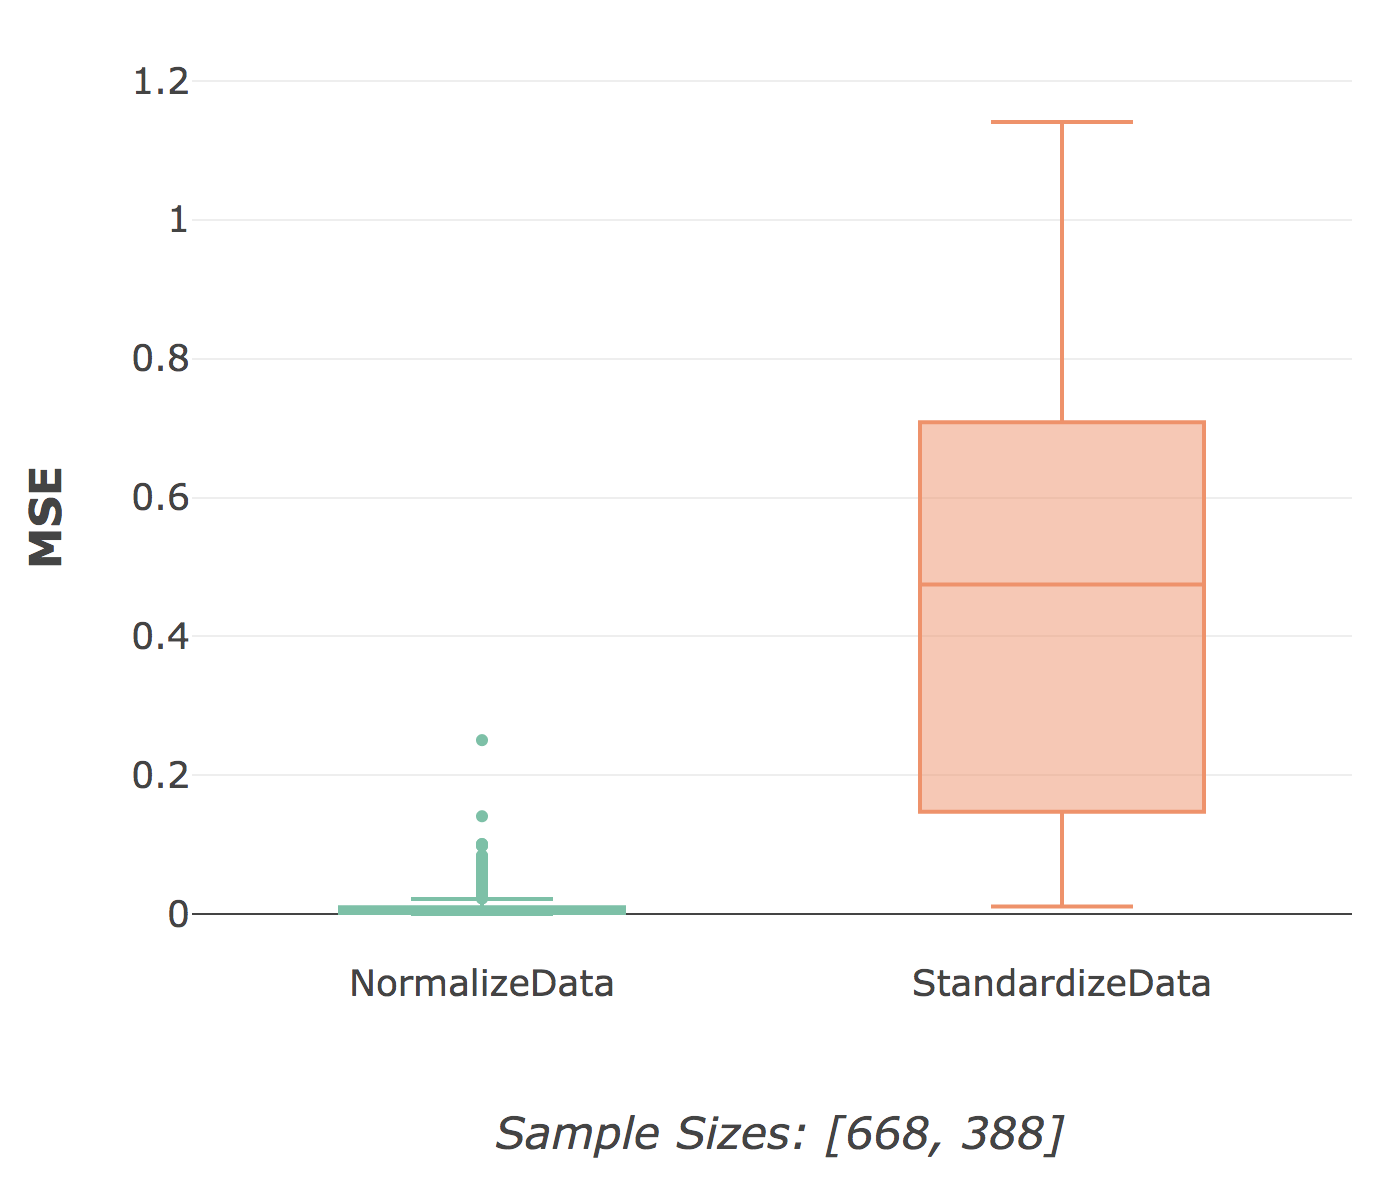
\includegraphics[scale=0.25]{images/results/activations/actual_mse_scaling.png}
		\caption{\textbf{Scaling Technique} 
			\newline }
		\label{figure-actual_mse_scaling}
	\end{subfigure}%
	\begin{subfigure}{.5\textwidth}
		\centering 
		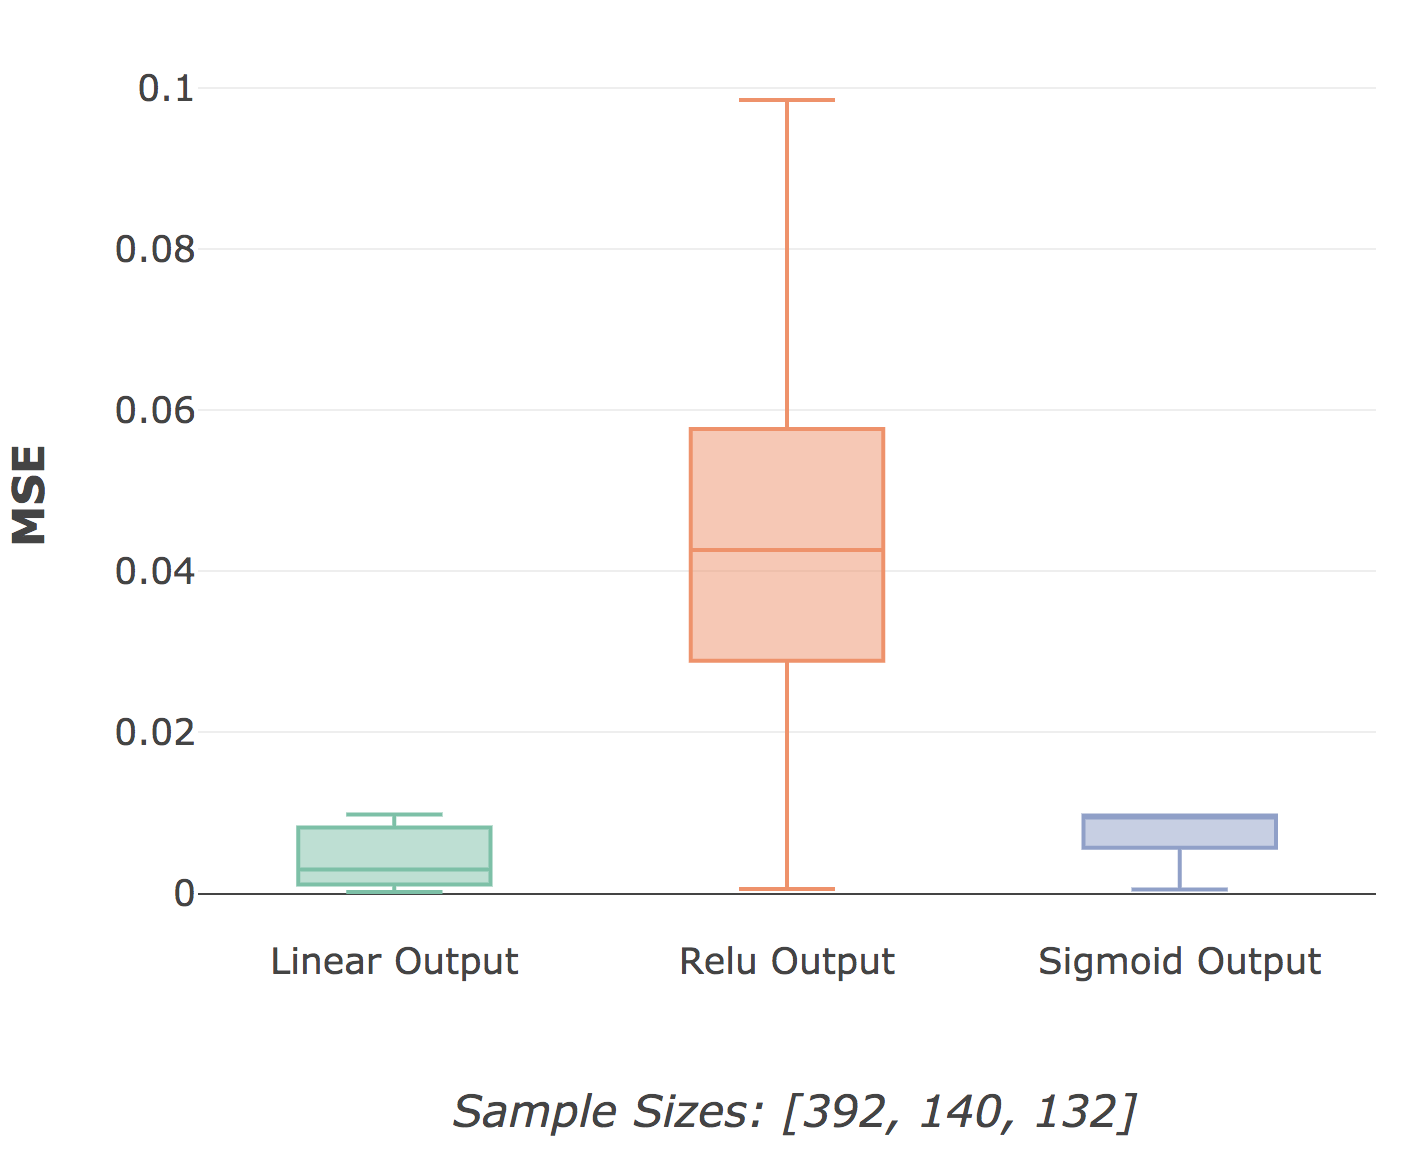
\includegraphics[scale=0.25]{images/results/activations/actual_mse_output.png}
		\caption{\textbf{Output Activation} 
			\newline }
		\label{figure-actual_mse_output}
	\end{subfigure}
	\caption{Dataset: Scaling10 dataset (\ref{dataset_scaling10}), Configuration
		\newline Figure (a) here shows SAE MSE performance according to the scaling techniques as described in \ref{data_scaling}. As discussed more fully in \ref{proc_dataprep}, the use of standardization for scaling the data doesn't allow for effective outlier treatments, resulting in the significantly worse performance seen here.
		\newline Figure (b) shows the effects of the output activation for configurations using Normalized scaling. The ReLU activations also seemed to result in very poor performance, most likely due to the loss of error signal in the output layer where it is most critical. }
	\label{figure-mse_scaling}
\end{figure}


\begin{figure}[H]
	\centering
	\textbf{MSE by Activations and Encoding Layer Size}
	\begin{subfigure}{.5\textwidth}
		\centering 
		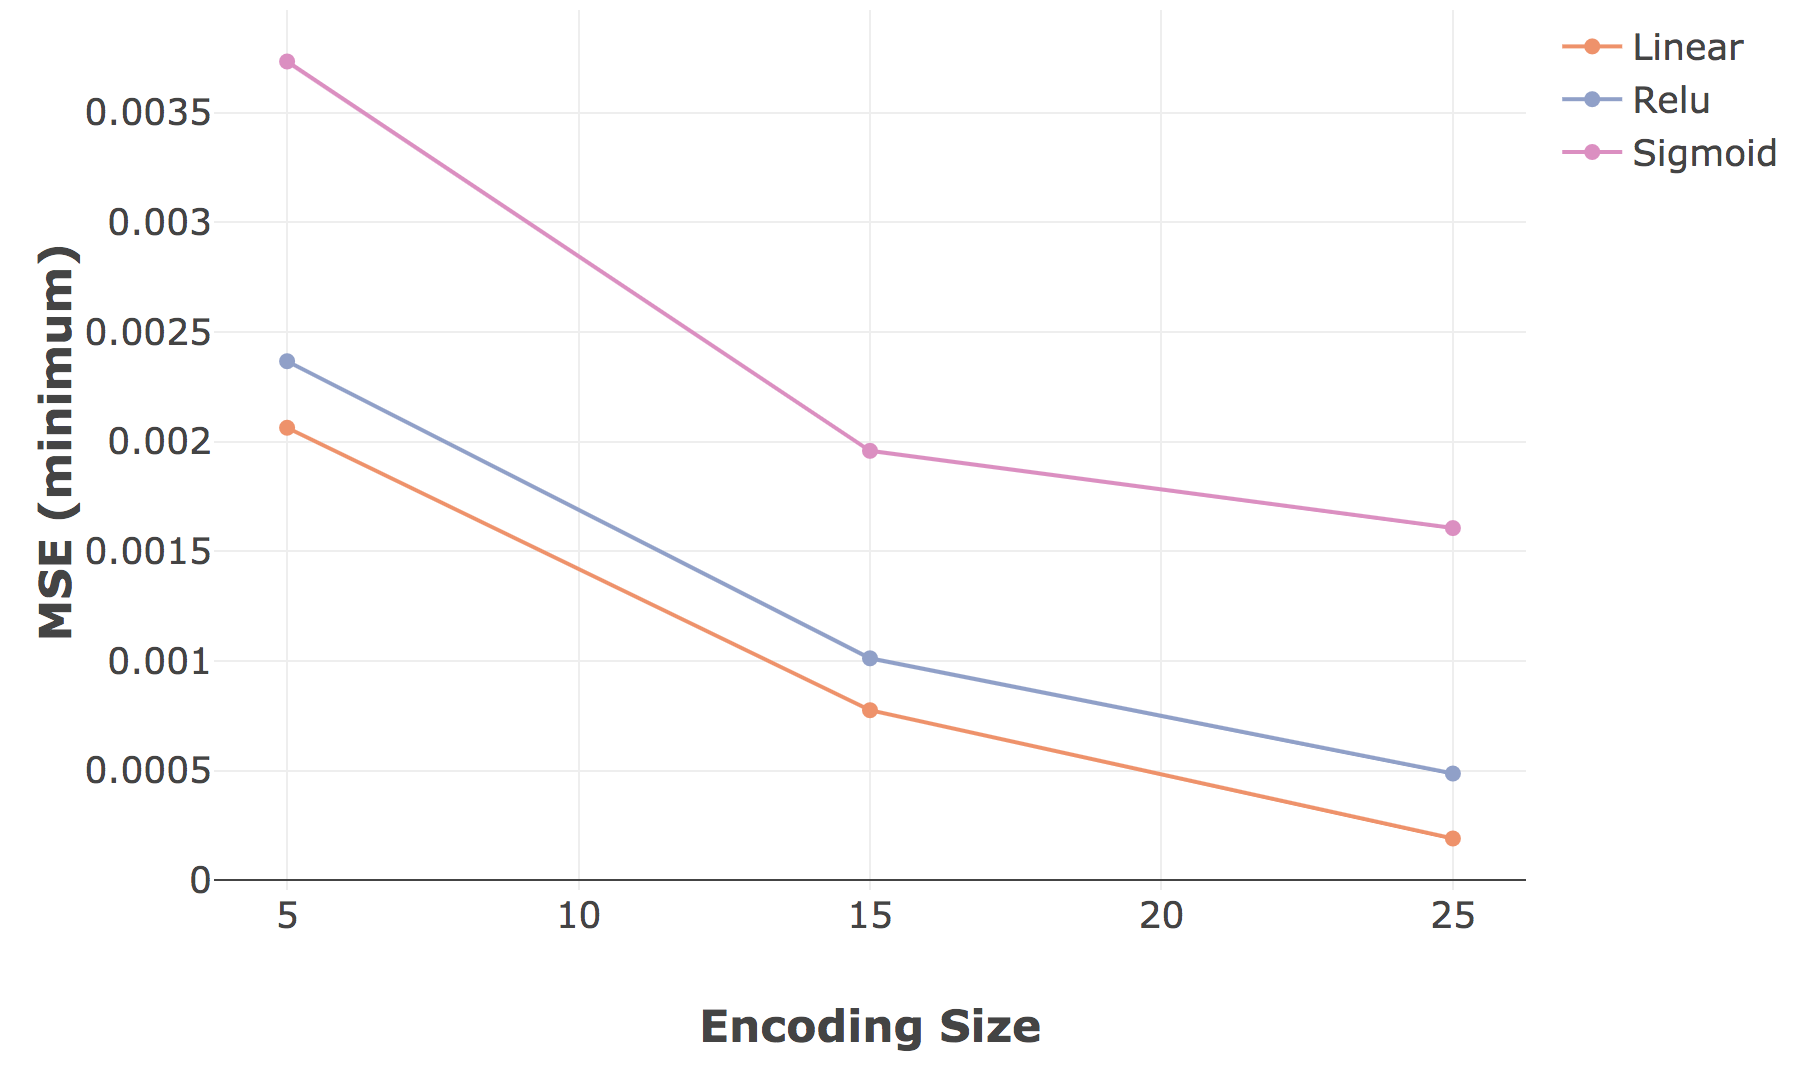
\includegraphics[scale=0.25]{images/results/activations/actual_mse_encoding.png}
		\caption{\textbf{Encoding Activations} 
			\newline }
		\label{figure-actual_mse_encoding_activations}
	\end{subfigure}%
	\begin{subfigure}{.5\textwidth}
		\centering 
		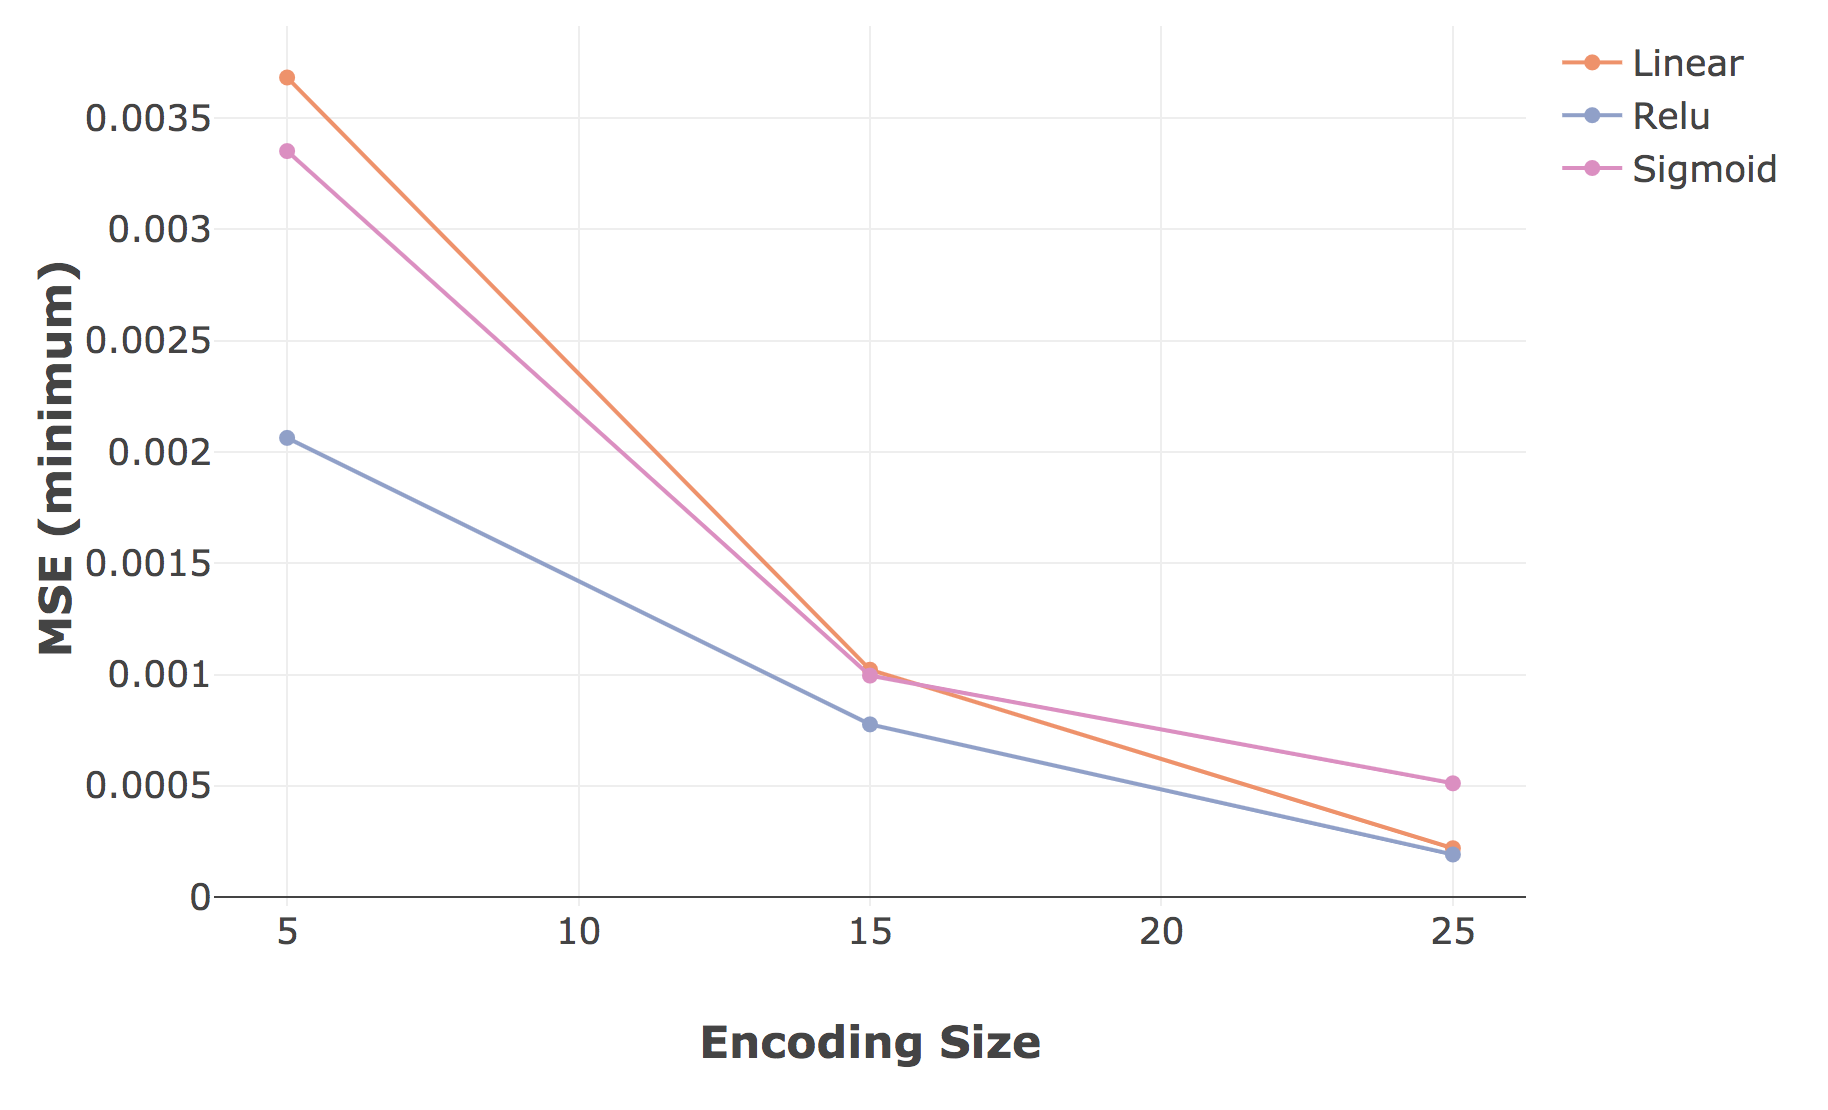
\includegraphics[scale=0.25]{images/results/activations/actual_mse_hidden.png}
		\caption{\textbf{Hidden Activations} 
			\newline }
		\label{figure-actual_mse_hidden_activations}
	\end{subfigure}
	\caption{Dataset: Scaling10 dataset (\ref{dataset_scaling10}), Configuration
		\newline Figure (a) shows the best (minimum) MSE scores for different encoding activations at the different encoding layer sizes (with a network input of 30). There is a consisent out performance of Linear activations in the encoding layer, which usual to expected from literature \cite{Hinton2}, and in line with reducing loss of error signal at critical points. 
		\newline Figure (b) shows the best (minimum) MSE scores for different hidden layer activations at the different encoding layer sizes (with a network input of 30). At larger encoding layers, there is a competitive performance from all linear networks, where they are less pressured to take advantage of non-linear effects. As the size of the encoding layer is reduced, the advantages of non-linear activations become more apparent, with outperformance by ReLU and Simgoid activations. Sigmoid activations are known to suffer from learning slow down as a result of saturation and so have increased sensitivity to vanishing gradients \cite{Glorot2}. SAE networks are deep by nature, and so it is not surprising that the Sigmoid activations are resulting in worse performance over the same training period when compared to ReLU activations. \newline}
	\label{figure-mse_encoding_activations}
\end{figure}


\subsubsection{Predictive FFN Activations and Scaling}

In Figure \ref{figure-pl_activations_scaling}, a comparison scaling techniques as well as of Linear and ReLU activations are made for synthetic data in both smaller and larger sized networks. In line with the characteristics of the synthetic data noted in \ref{results_gbm_data}, results for networks using a Linear Activation often outperformed the networks using non-linear activations such as ReLU or Leaky ReLU (activation functions are detailed in \ref{imp_activation_functions}). \newline


\begin{figure}[H]
	\centering
	\textbf{P\&L by Scaling and Activations (Synthetic Data)}
	\begin{subfigure}{.5\textwidth}
		\centering 
		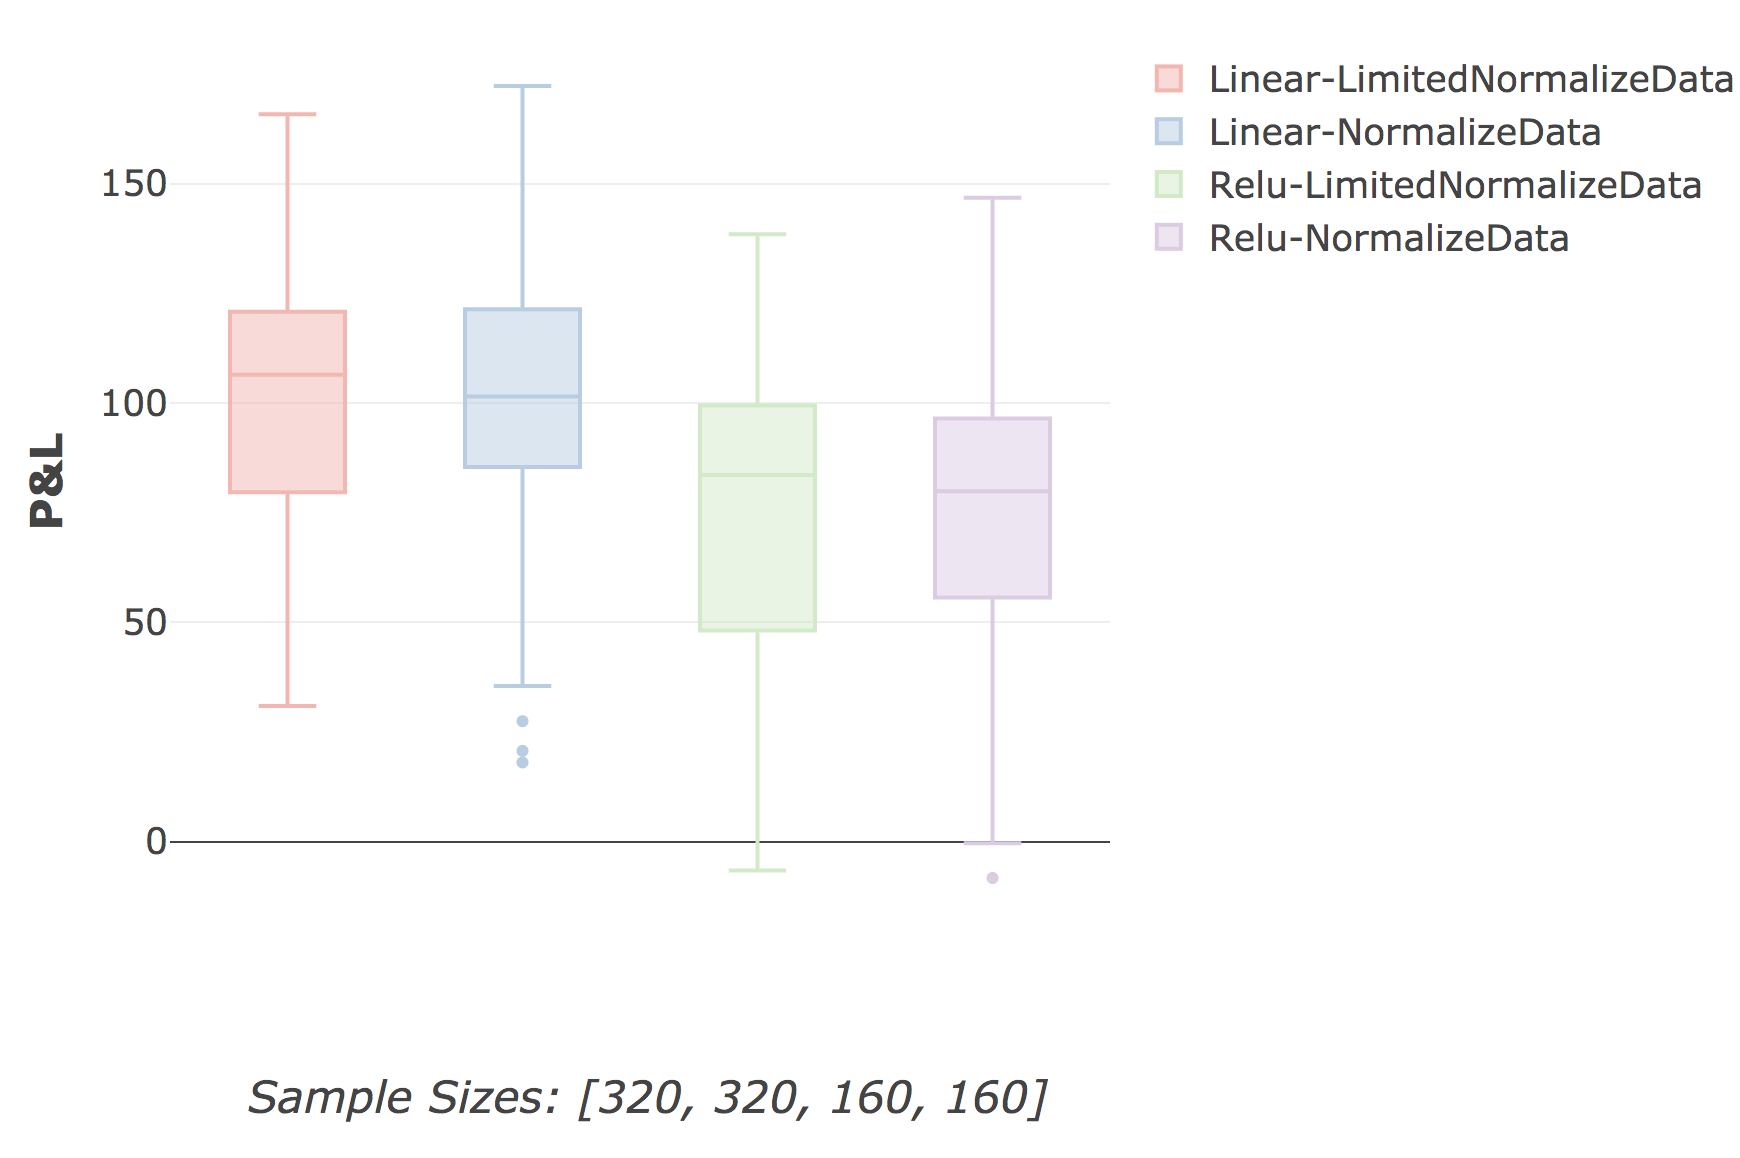
\includegraphics[scale=0.25]{images/results/activations/synth_pl_scaling.png}
		\caption{\textbf{Encoding Activations} 
			\newline }
		\label{figure-synth_pl_scaling}
	\end{subfigure}%
	\begin{subfigure}{.5\textwidth}
		\centering 
		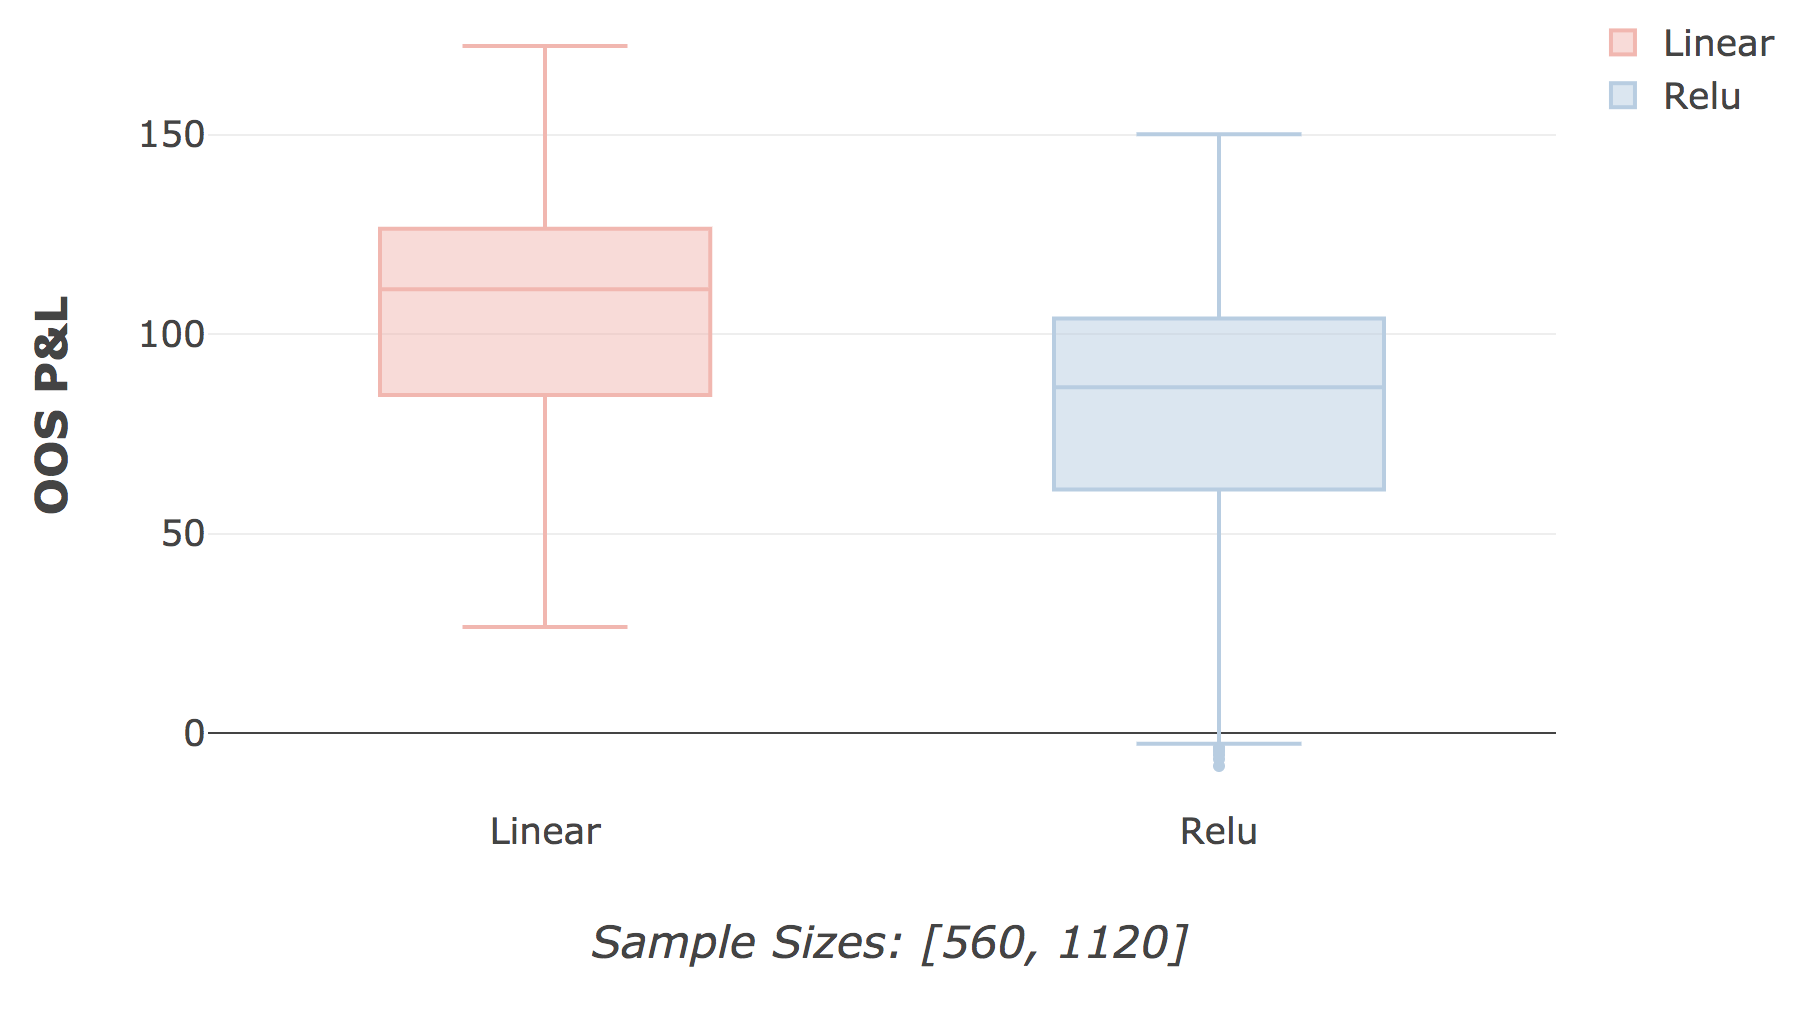
\includegraphics[scale=0.25]{images/results/activations/synth_pl_hidden.png}
		\caption{\textbf{Hidden Activations} 
			\newline }
		\label{figure-synth_pl_hidden}
	\end{subfigure}
	\caption{Dataset Synthetic6  (\ref{dataset_synthetic6})), Configuration
		\newline Figure (a) shows the impact of the limited scaling technique (as described in \ref{data_scaling}) in comparison to the non-limited version. The implementation of this is not a choice when interested in simulating a real world implementation, but it is still of interest to note the impact of this issue. Additionally, the use of a Linear output layer has been shown to assist in reducing the impact of this effect.
		\newline Figure (b) offers a comparison of Linear and ReLU hidden layer activations on P\&L, with the linear activations resulting in notably better P\&L when compared to ReLU activations. Unlike the SAE networks, this persists even when the network size is decreased - this difference highlights the effects of GBM data and that it can be represented linearly, as per \ref{results_gbm_data}, whereas we would see actual stock data to benefit from a non-linear representation. Linear configurations for actual data were not run, as real stock data is not expected to follow patterns that are linear through time, thus offering little value.}
	\label{figure-pl_activations_scaling}
\end{figure}



\subsubsection{Leaky ReLU vs ReLU}

Leaky ReLU activations were implemented, and showed negligible effects for SAE, which can be seen in the Appendix \ref{results_activations_appendix}. For the predictive network, the LeakyReLU did offer some more significant improvements, as seen in Figured \ref{figure-synthetic_pl_leakyrelu} below, and so has been used as the hidden layer activation of choice for subsequent experiments.

\begin{figure}[H]
	\textbf{P\&L by ReLU Activations (Synthetic Data)}
	\centering
	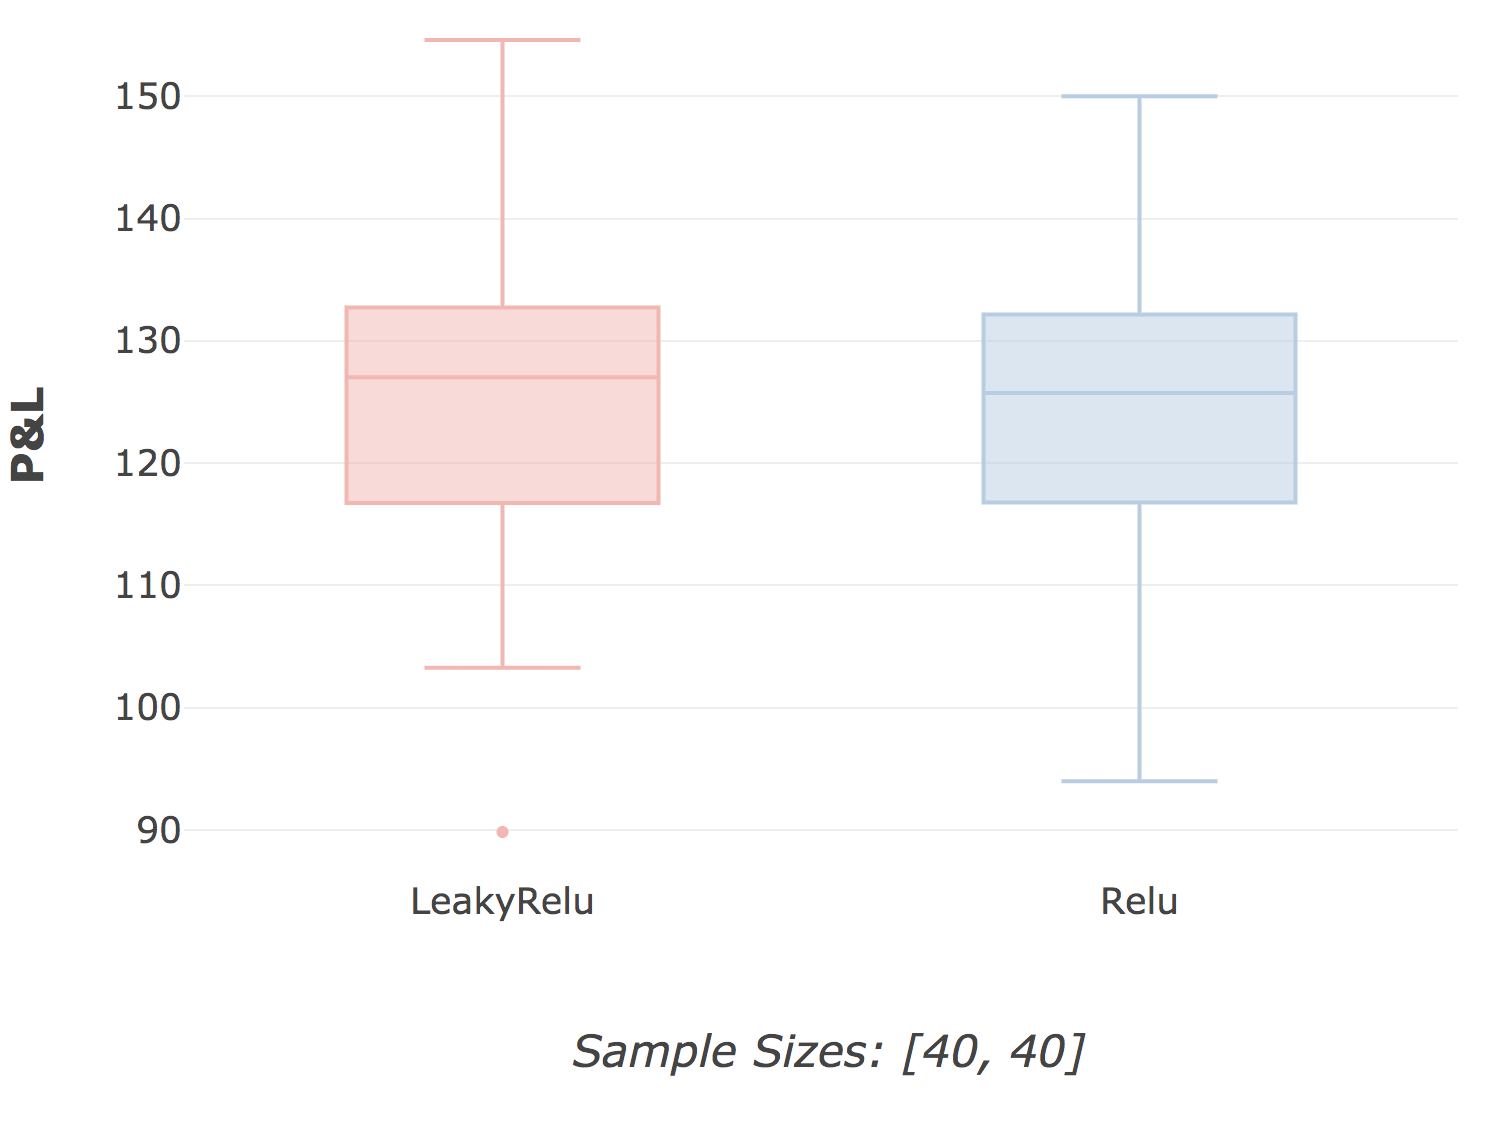
\includegraphics[scale=0.3]{images/results/activations/synthetic_pl_leakyrelu.png}
	\caption{Dataset Synthetic6  (\ref{dataset_synthetic6}) ; Configuration 
		\newline The plot shows the FFN P\&L, grouped by activation, showing some improvements from the Leaky ReLU activation. The effect is most noticeable in reducing the lower bounds of performance (±10.8\%), though has a clear benefit in the upper bounds as well (3.4\%).}
	\label{figure-synthetic_pl_leakyrelu}
\end{figure}

\newpage
\subsection{Weight Initialization Techniques}\label{results_init}

\subsubsection{RBM Pretraining for Sigmoid Networks}

While previously considered the best approach for training deep neural networks, the methodology of greedy layerwise RBM pre-training for Sigmoid SAE networks (as described in \cite{Hinton2}) had detrimental effects on network performance, as seen below in Figure \ref{figure-results-pretraining-effect}. \newline

\begin{figure}[H]
	\centering
	\textbf{Pre-training Effects on SAE MSE Scores (Actual Data)} 
	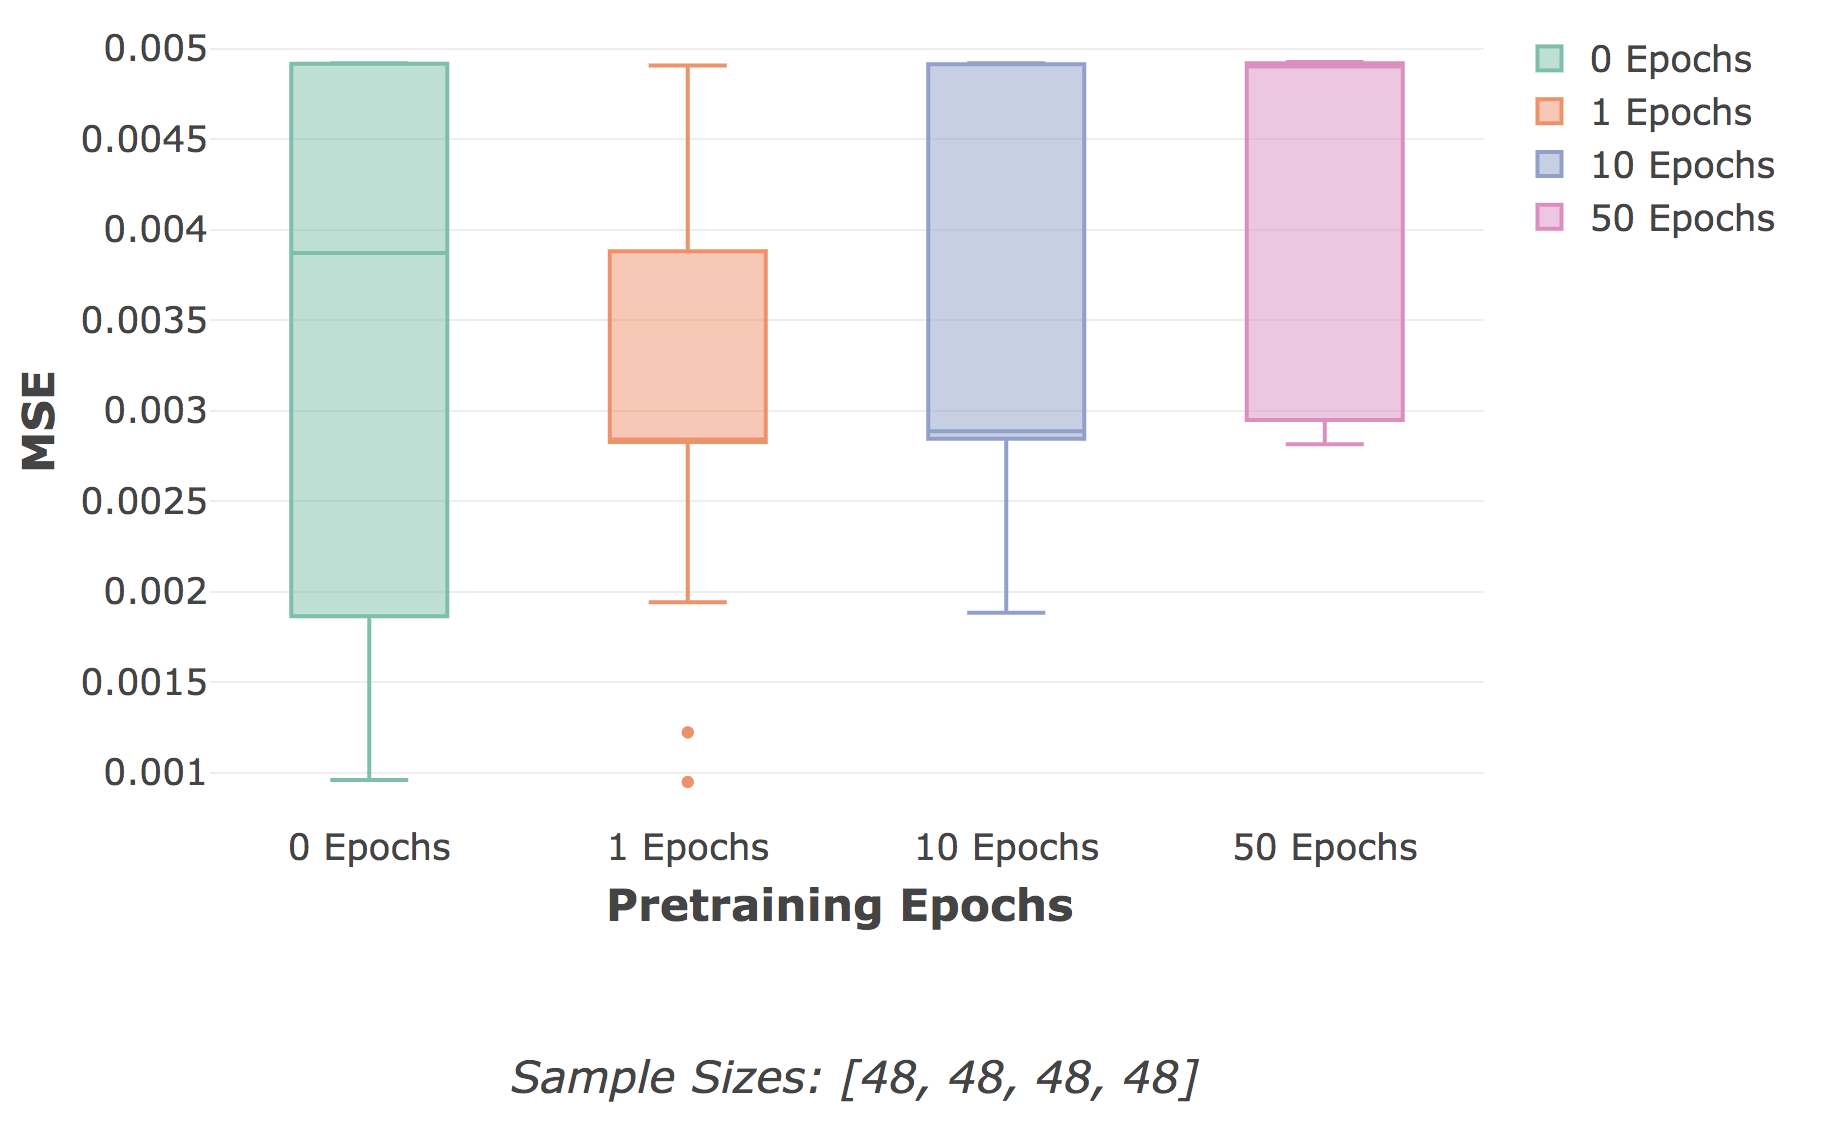
\includegraphics[scale=0.32]{images/results/newinit/actual_sigmoid_pt.png}
	\caption{Dataset AGL\&ACL (\ref{dataset_aglacl}); Configuration7 (\ref{config7})
		\newline \newline The boxplots here show the summary of configuration performances, by minimum MSE achieved, grouped according to the number of pre-training epochs which the network had. There is a clear favour to having no pre-training in this scenario as there is a clear decrease in performance as the number of epochs increase (the low value outliers that can be seen for the 1 epoch configuration were with learning rates which were low enough to approximate no epochs).}
	\label{figure-results-pretraining-effect}
\end{figure}		

The RBM pre-training technique does assume that data is Independent and Identically Distributed (IID), and does ultimately traverse a different solution space and loss function. While it may be effective in some contexts, it was shown to result in a counterproductive exploration of the weight space for this non-IID dataset, and that ultimately the financial time series data is pathological for RBM pre-training. It may also emphasise the value of more recent data over historical data usage, as discussed more in Section \ref{results_hist}\footnote{The RBM greedy layerwise training implementation was effectively tested and validated on known datasets such as MNIST, example results for which can bee seen in Section of the Appendix}.\newline 

\paragraph{Sigmoid Activation Functions} 
Due to the poor performance seen in Sigmoid function based SAE's here, as well as the poorer results when compared to ReLU activations (noted in \ref{results_activations_scaling}), Sigmoid functions were largely excluded from further configuration testing.


\subsubsection{Variance Based Weight Initialization Techniques}

More recent research has focused on the use of weight initialization using variance based methodologies, as discussed fully in \ref{imp_weights}. Our expectation, theoretically, is that the He initialization will generally outperform Xavier due to it being more appropriate for the ReLU activations being used. Additionally, in networks with varying layer sizes, we expect He-Adj and possibly Xavier to outperform He which is subject to imbalanced initializations. Ultimately, He-Adj as presented in \ref{imp_weights}, should present the best of both for an initialization that is suited to Leaky ReLU activations and the varying layer sizes found in SAE networks.\newline

Training SAE networks across the Synthetic10 (\ref{dataset_synthetic10}), Actual10 (\ref{dataset_actual10}) and AGL (\ref{dataset_agl}) datasets, we mostly see the expected patterns emerge. He-Adj consistently outperforms He due to being better suited to the network structures, as seen in figures \ref{figure-results_it4_sae_init}, \ref{figure-results_init_actual10_all} and \ref{figure-results_init_agl_all} below. We also see that He-Adj clearly outperforms Xavier for actual data in figures \ref{figure-results_init_actual10_all} and \ref{figure-results_init_agl_all}, but has performance that is mostly the same (or even marginally worse) than Xavier for the synthetic dataset in figure \ref{figure-results_it4_sae_init}. \newline

As discussed more fully in \ref{results_linearity}, the GBM data in synthetic datasets will have assets that are configured to certain mean and variances. As these movements are aggregated over time through the data processing, the movements will generally be more similar and less complex than those of actual stock data which will show greater variance over time. The learning process then is not required to be able to pass through error signals that change as dynamically over time, and so there is less pressure on the initial starting weights. Additionally, He and He-Adj have a higher upper bound in the values used for Uniform distribution initialization than Xavier, and so are less likely to result in dying ReLU nodes from early learnings that are less representative of longer term patterns and so become damaging to final network performance. Further, some of the assumptions of these techniques, such as data being IID may not apply in the first place, making their results less predictable. These effects result in the outperformance of He-Adj in the networks trained on actual datasets, but similar performance of He-Adj and Xavier in the networks trained on synthetic data. \newline

\begin{figure}[H]
	\centering
	\textbf{Weight Initialization for SAE MSE - Synthetic10} 
	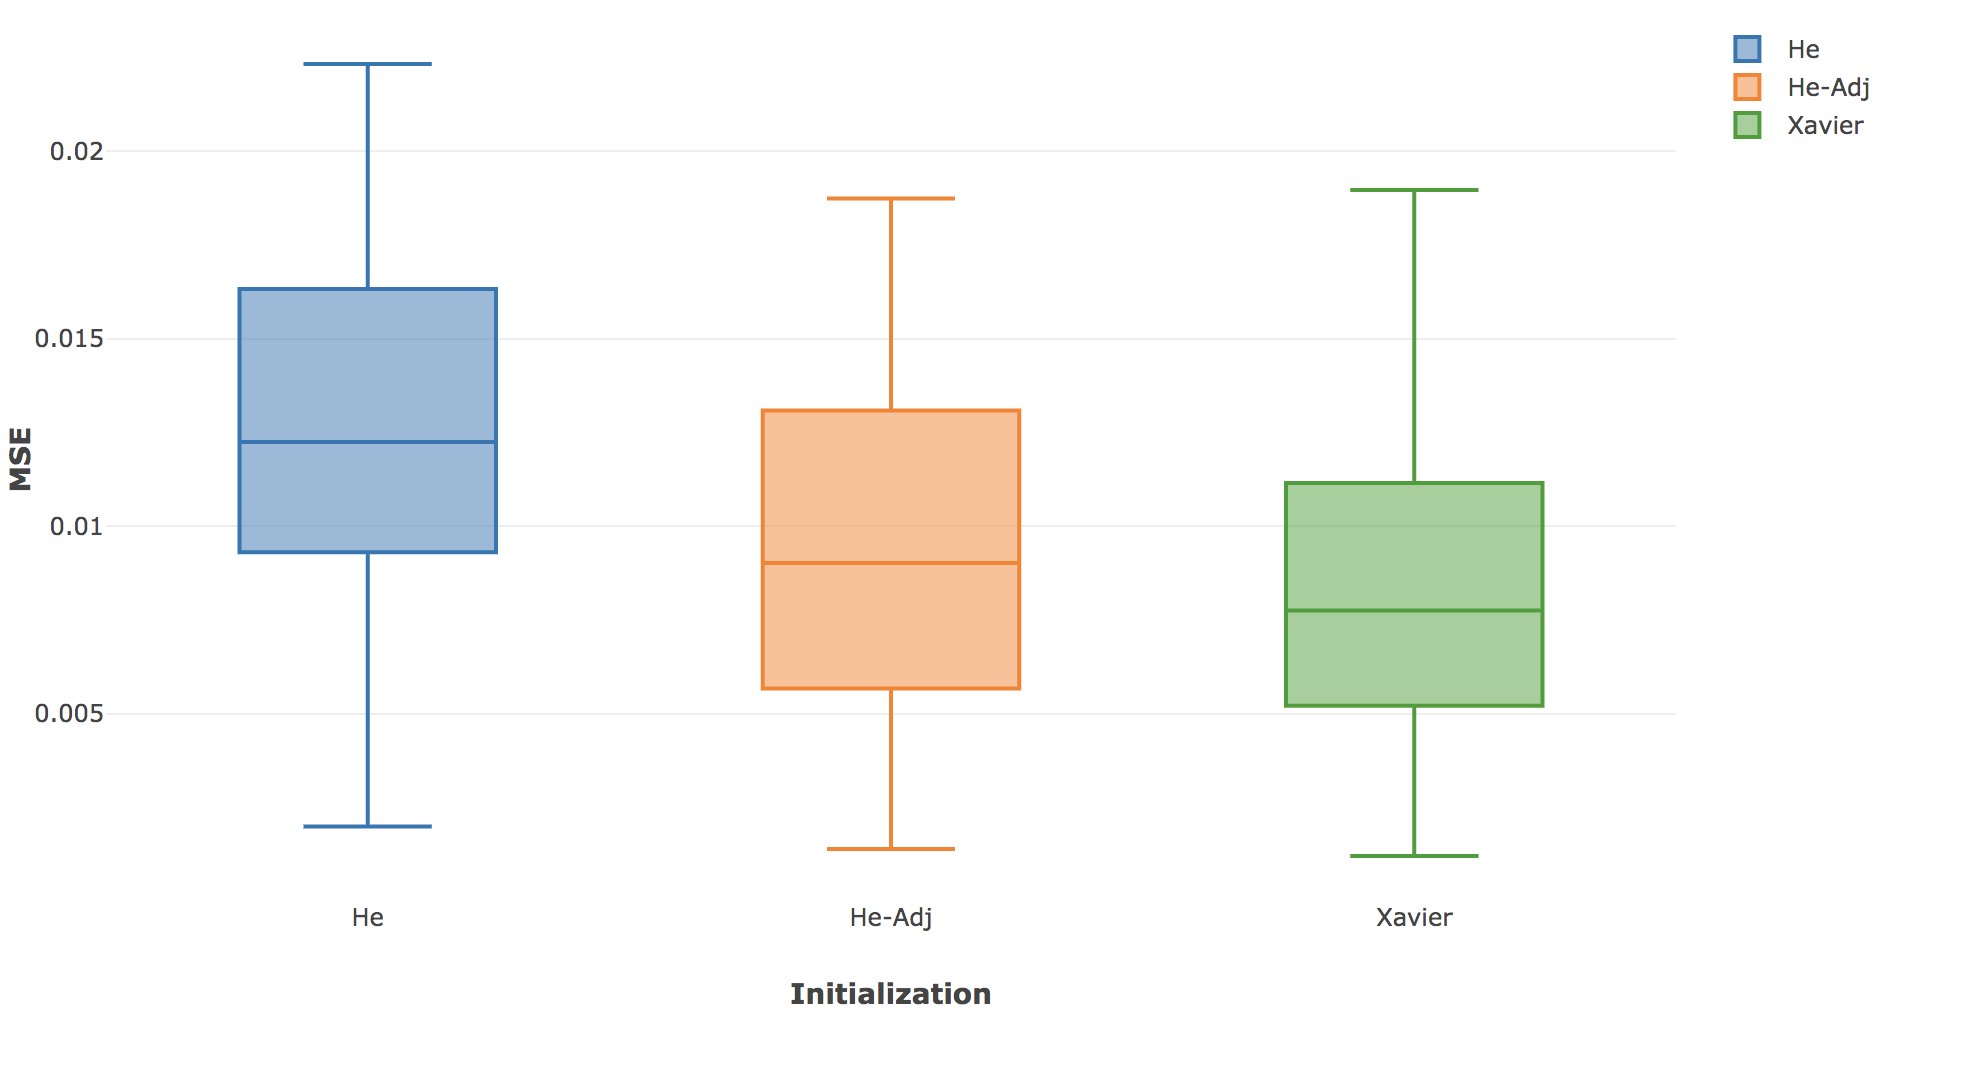
\includegraphics[scale=0.35]{images/results/init/Synthetic10_all.png}
	%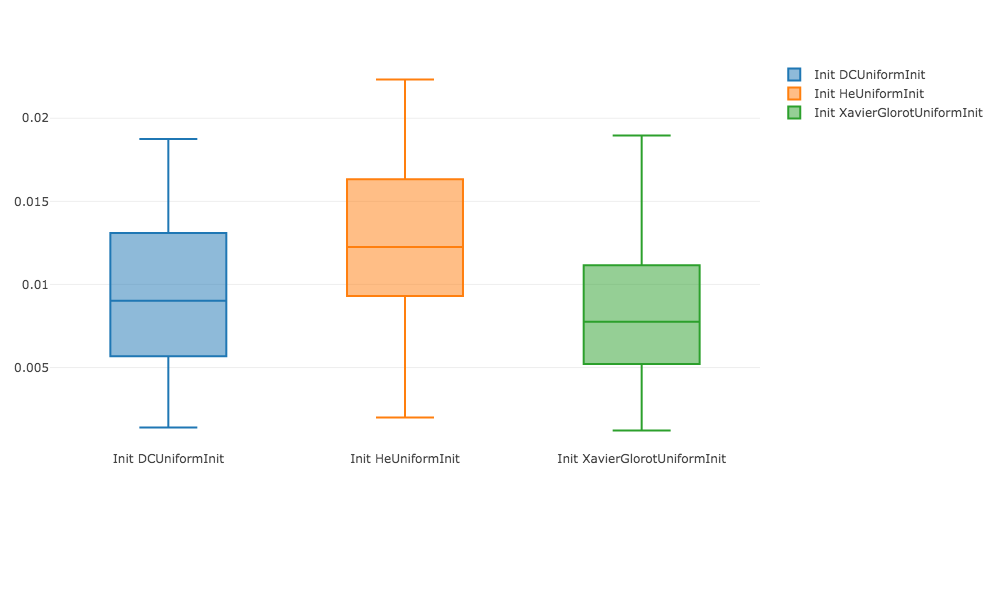
\includegraphics[scale=0.35]{images/iteration_four/it4_sae_init.png}
	\caption{Dataset: Synthetic10 (\ref{dataset_synthetic10}); Configuration 5 (\ref{config5})
		\newline The box plots show the MSE for a series of SAE networks trained, showing the outperformance of He-Adj compared to He in networks with changing layer sizes, and the similar performance of He-Adj and Xavier on synthetic datasets.}
	\label{figure-results_it4_sae_init}
\end{figure}

\begin{figure}[H]
	\centering 
	\textbf{Weight Initialization for SAE MSE - Actual10}
	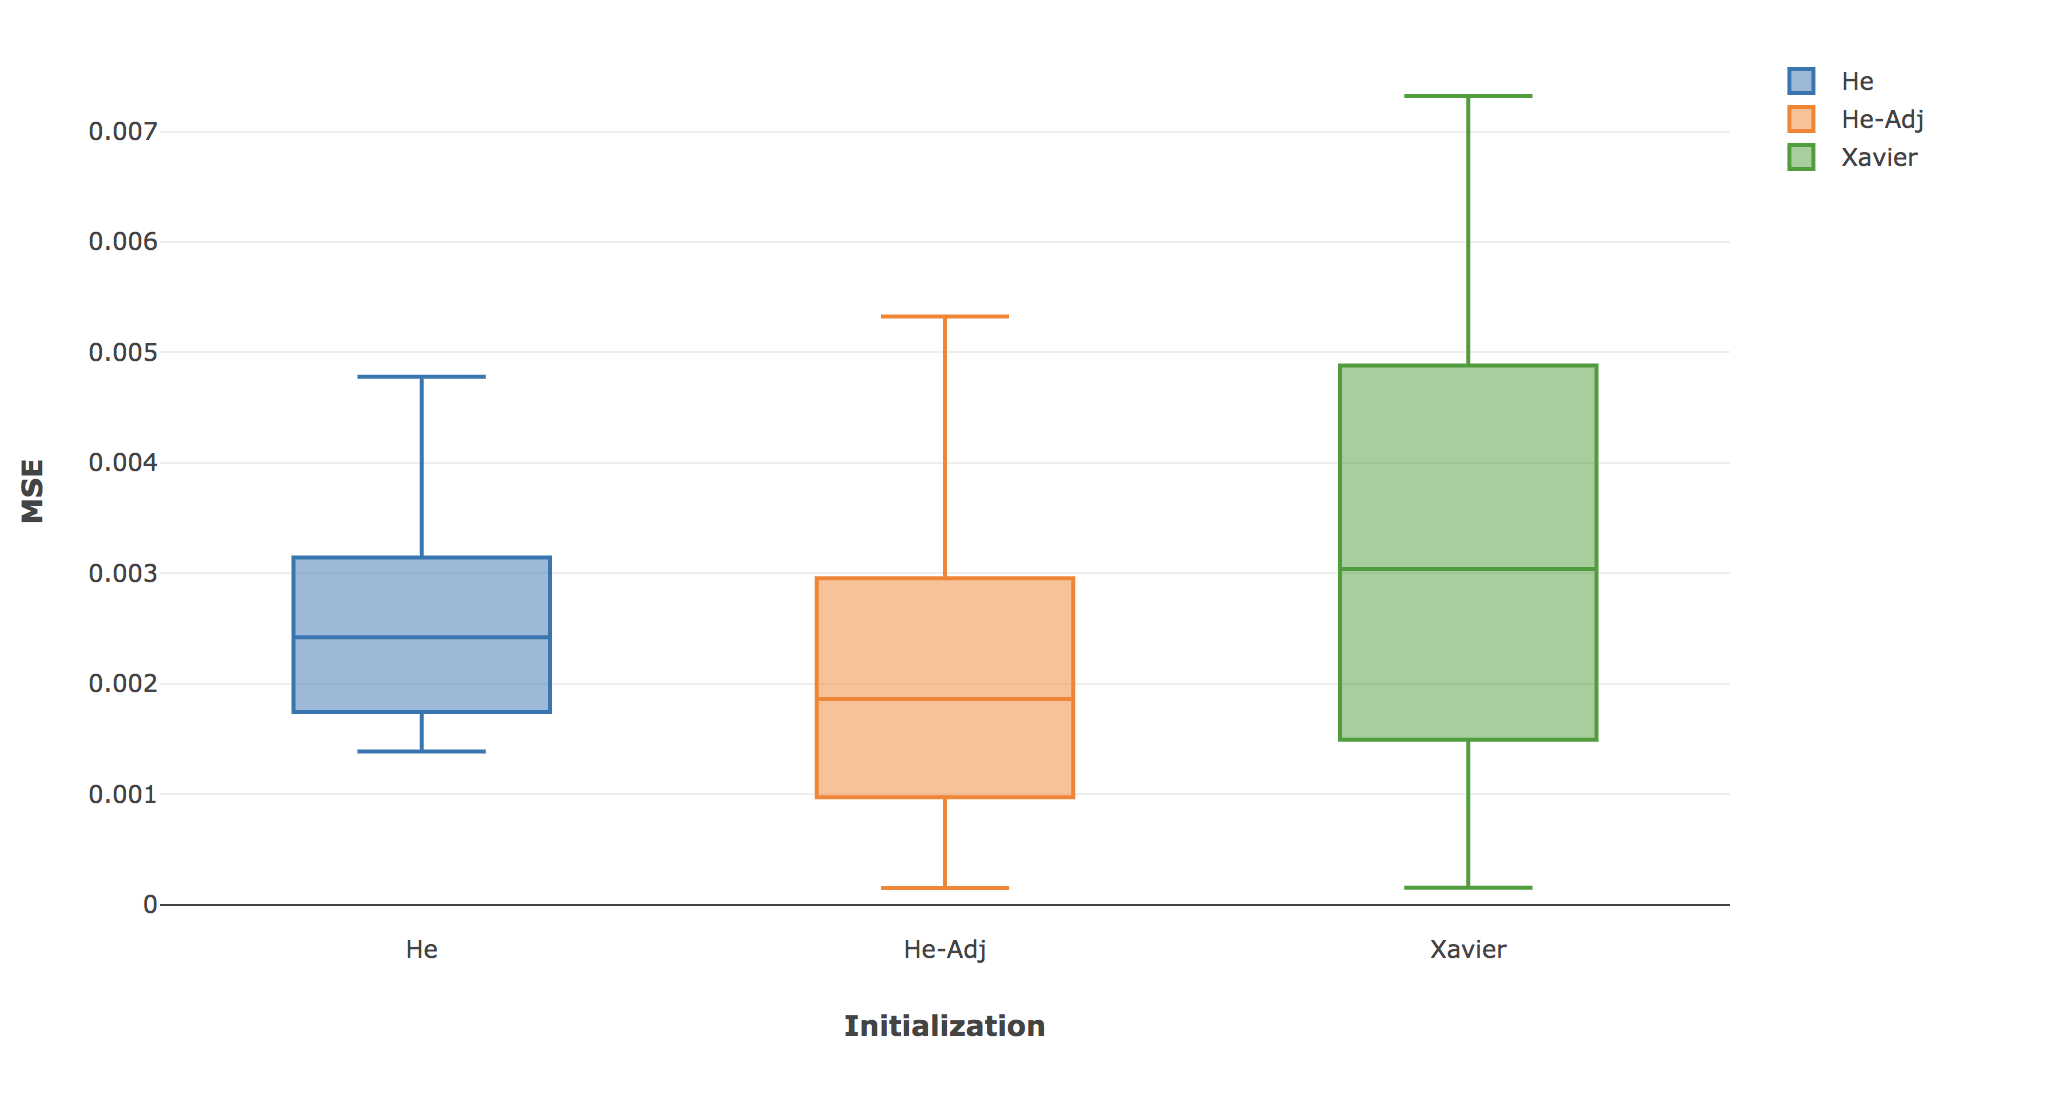
\includegraphics[scale=0.35]{images/results/init/Actual10_all.png} 
	%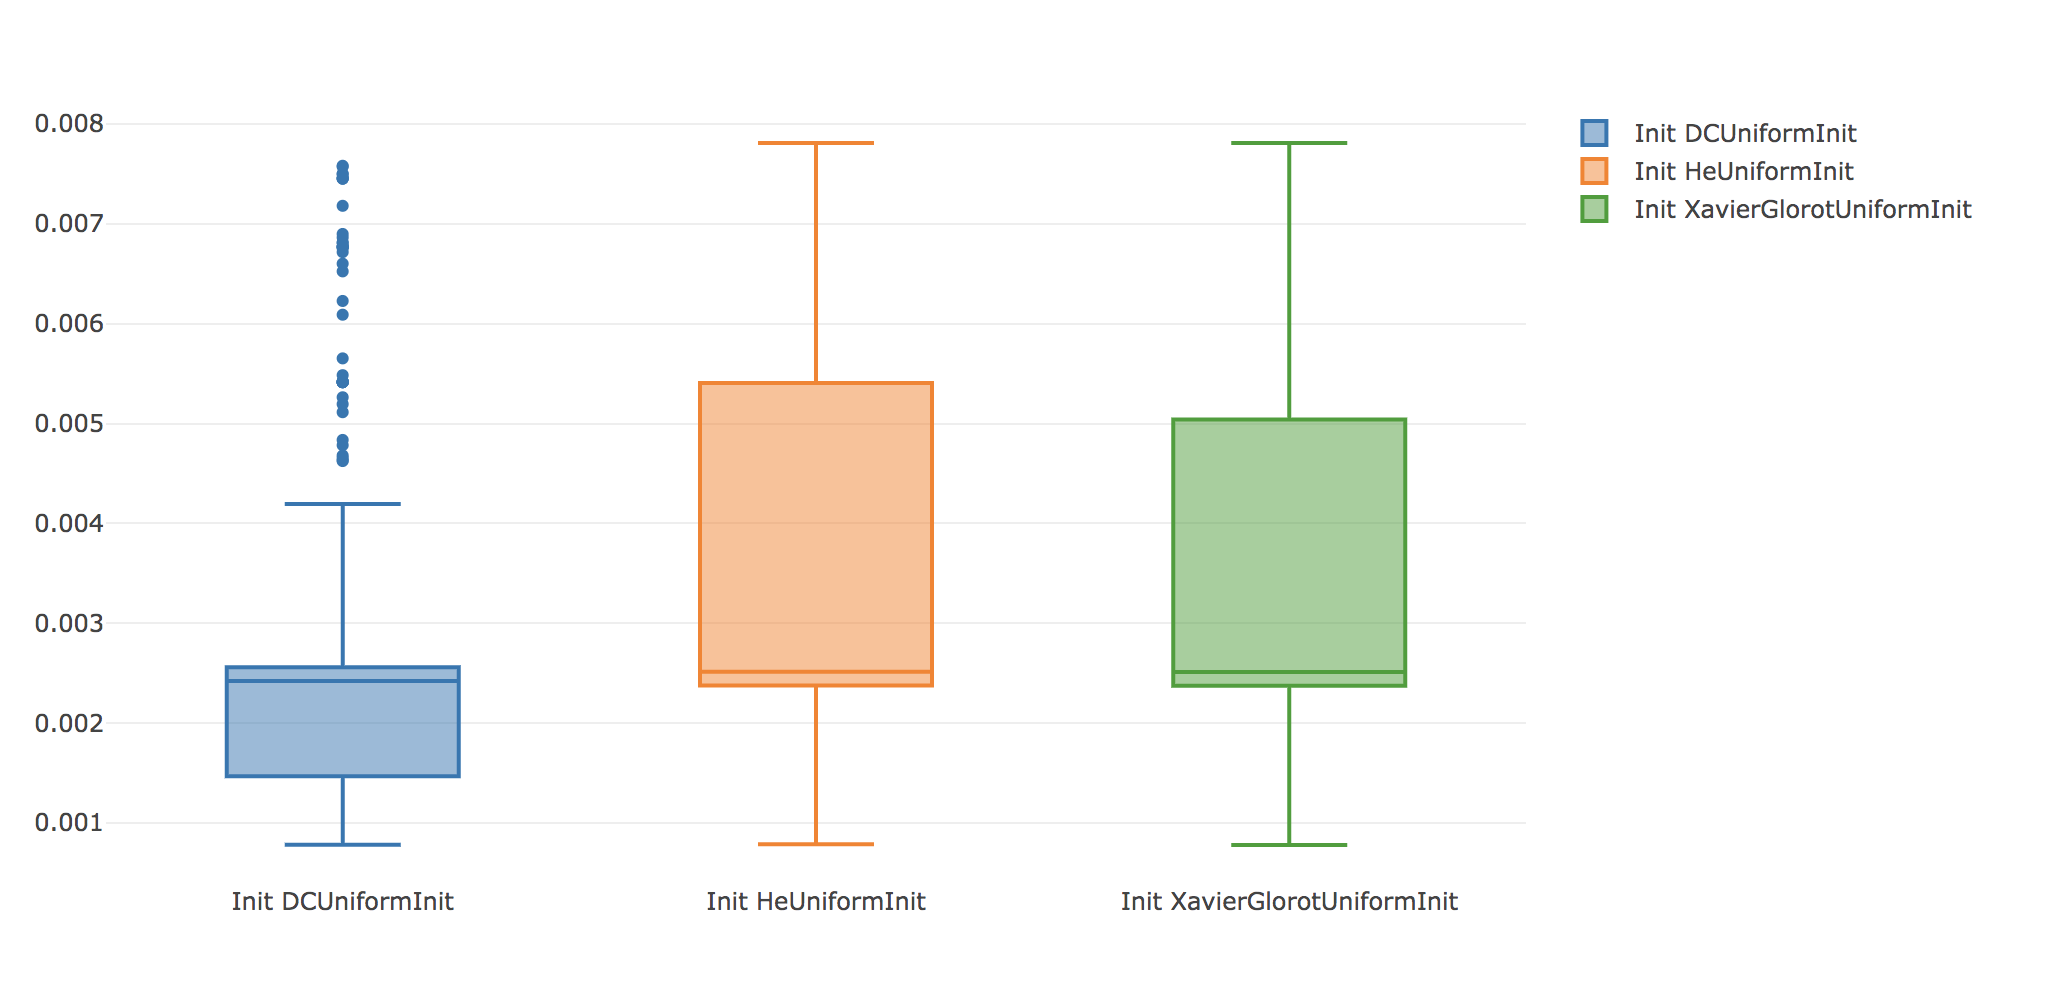
\includegraphics[scale=0.35]{images/iteration_five/it5_sae_init_agl.png}
	\caption{Dataset Actual10
		\newline The box plots show the MSE for a series of SAE networks trained, showing the outperformance of He-Adj compared to He in networks with changing layer sizes, and the  outperformance of He-Adj to Xavier on actual datasets.}
	\label{figure-results_init_actual10_all}
\end{figure}

\begin{figure}[H]
	\centering 
	\textbf{Weight Initialization for SAE MSE - AGL}
	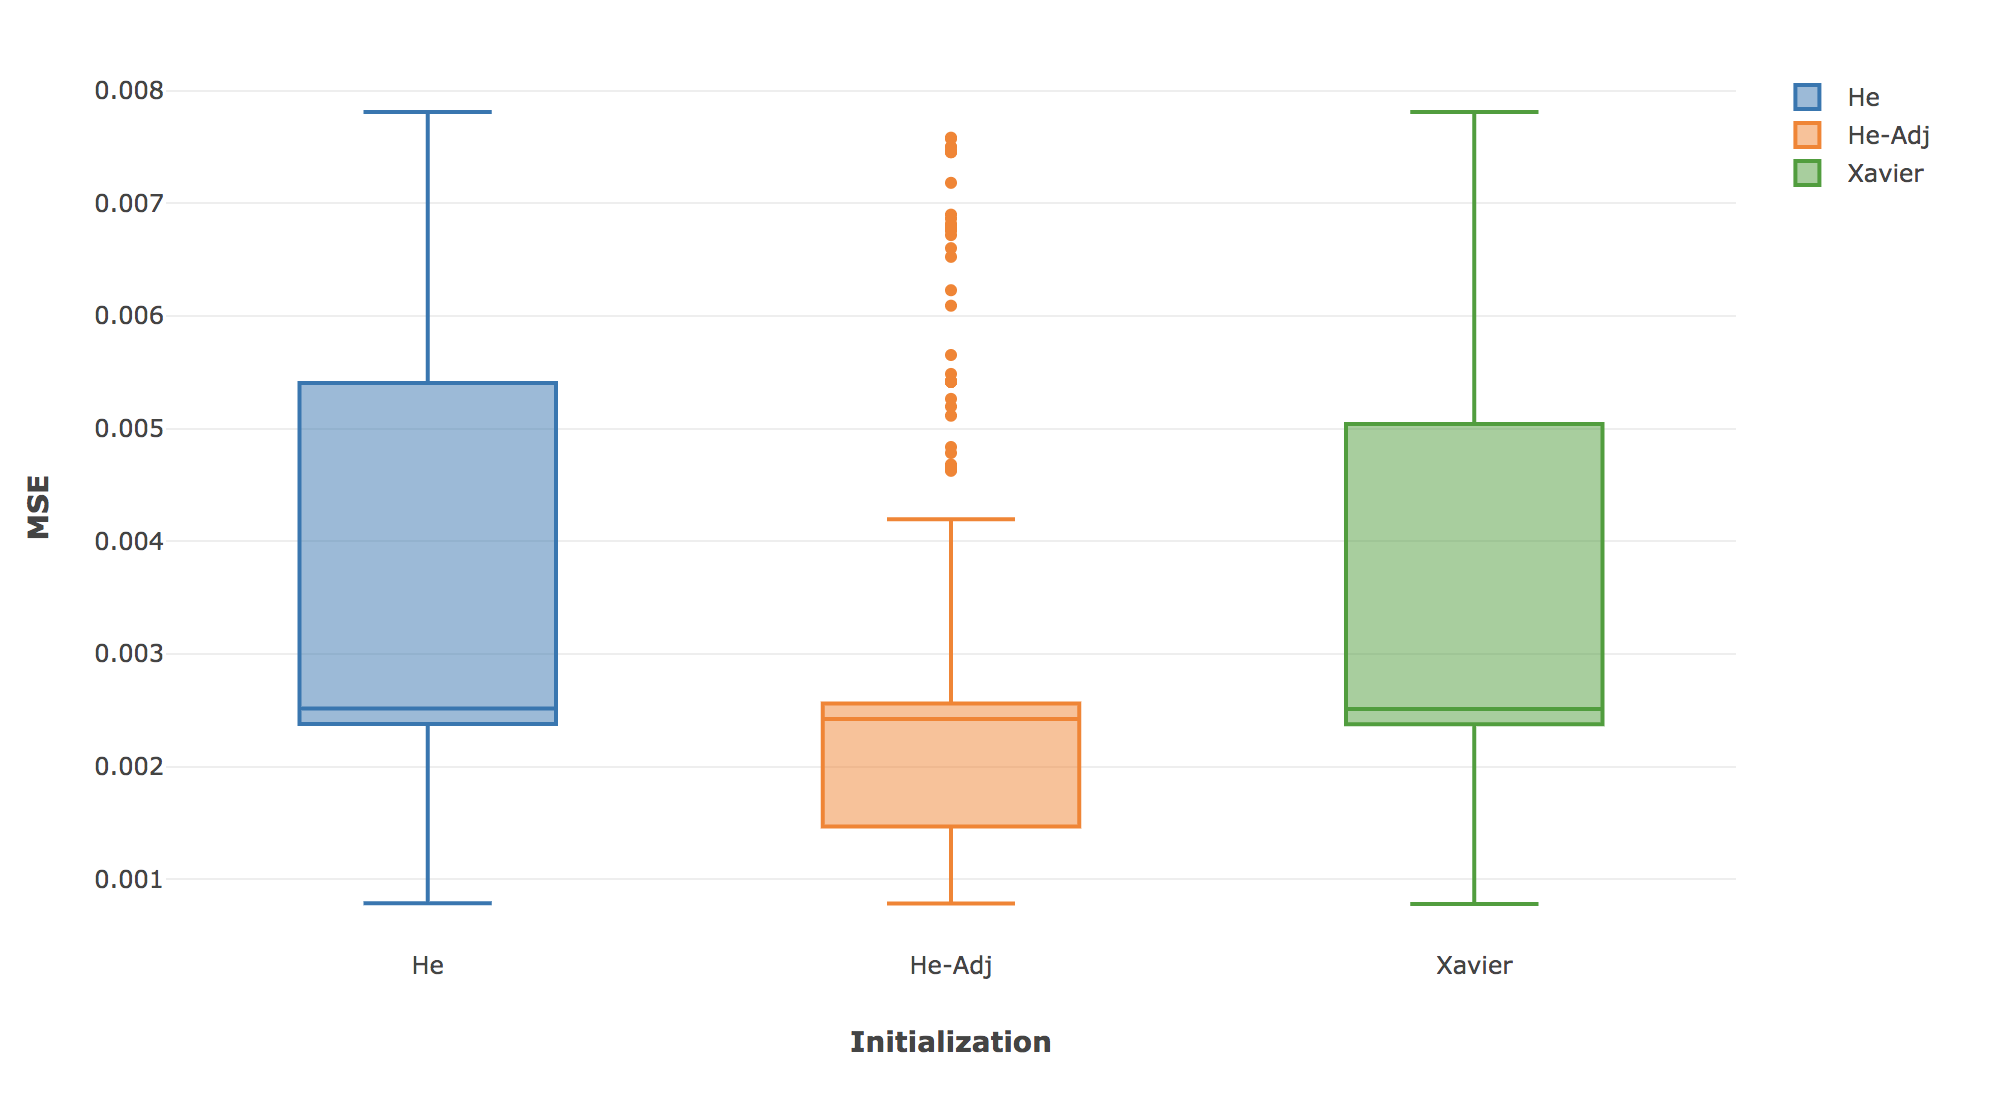
\includegraphics[scale=0.35]{images/results/init/AGL_all.png} 
	%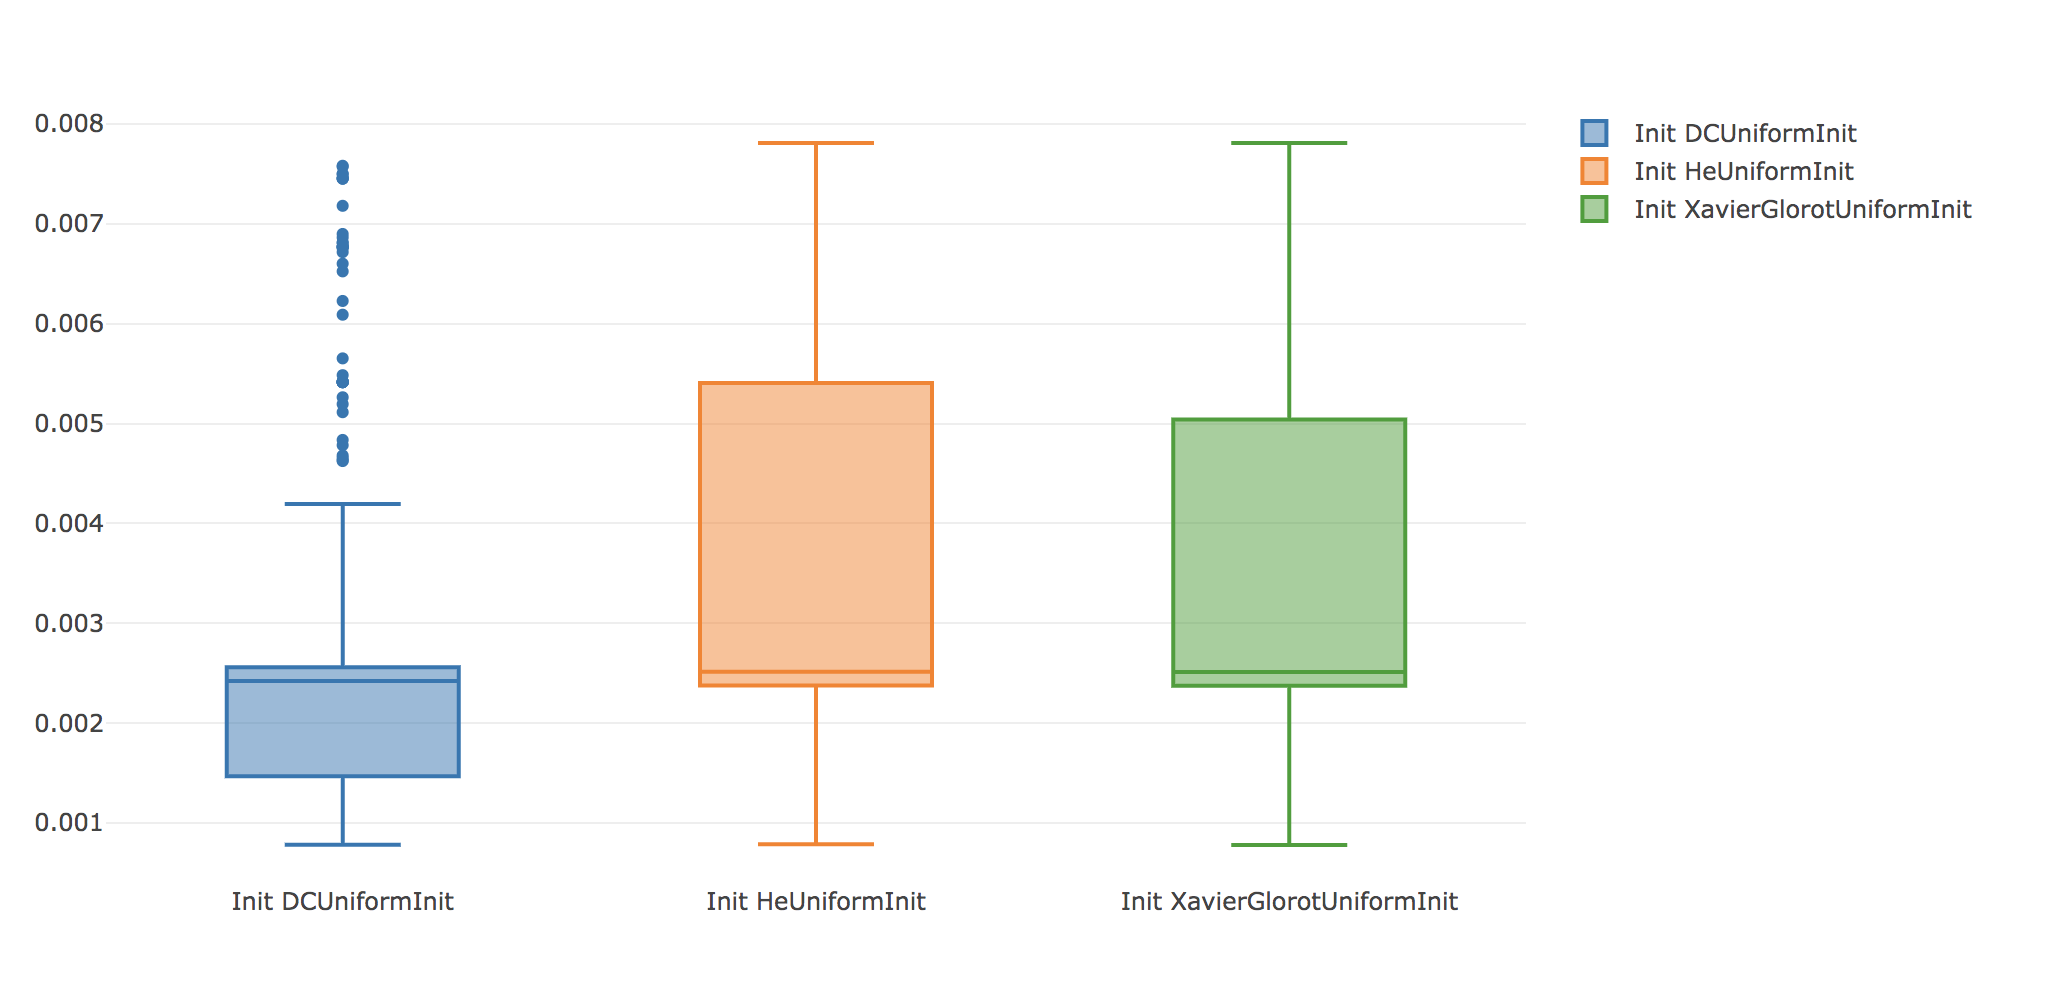
\includegraphics[scale=0.35]{images/iteration_five/it5_sae_init_agl.png}
	\caption{Dataset: AGL (\ref{dataset_agl}); Configuration 3 (\ref{config3})
		\newline The configurations run for AGL show notably better performance using the He-Adj based initialization in comparison to both He and Xavier. The emphasis seen here can be attributed to increased pressure on suitable weight initizliations as 1 and 2 node encoding layers were used.}
	\label{figure-results_init_agl_all}
\end{figure}


When considering the predictive FFN networks, with more consistent layer sizes, the performance between He and He-Adj becomes comparable, with both outperforming Xavier (as expected, with ReLU activations). Due to the generally better or comparable performance of He-Adj, it was the only initialization chosen for the Actual10 dataset, and so only AGL is presented for the predictive networks below.


\begin{figure}[H]
	\centering
	\textbf{Weight Initialization for Predictive FFN P\&L- Synthetic10}
	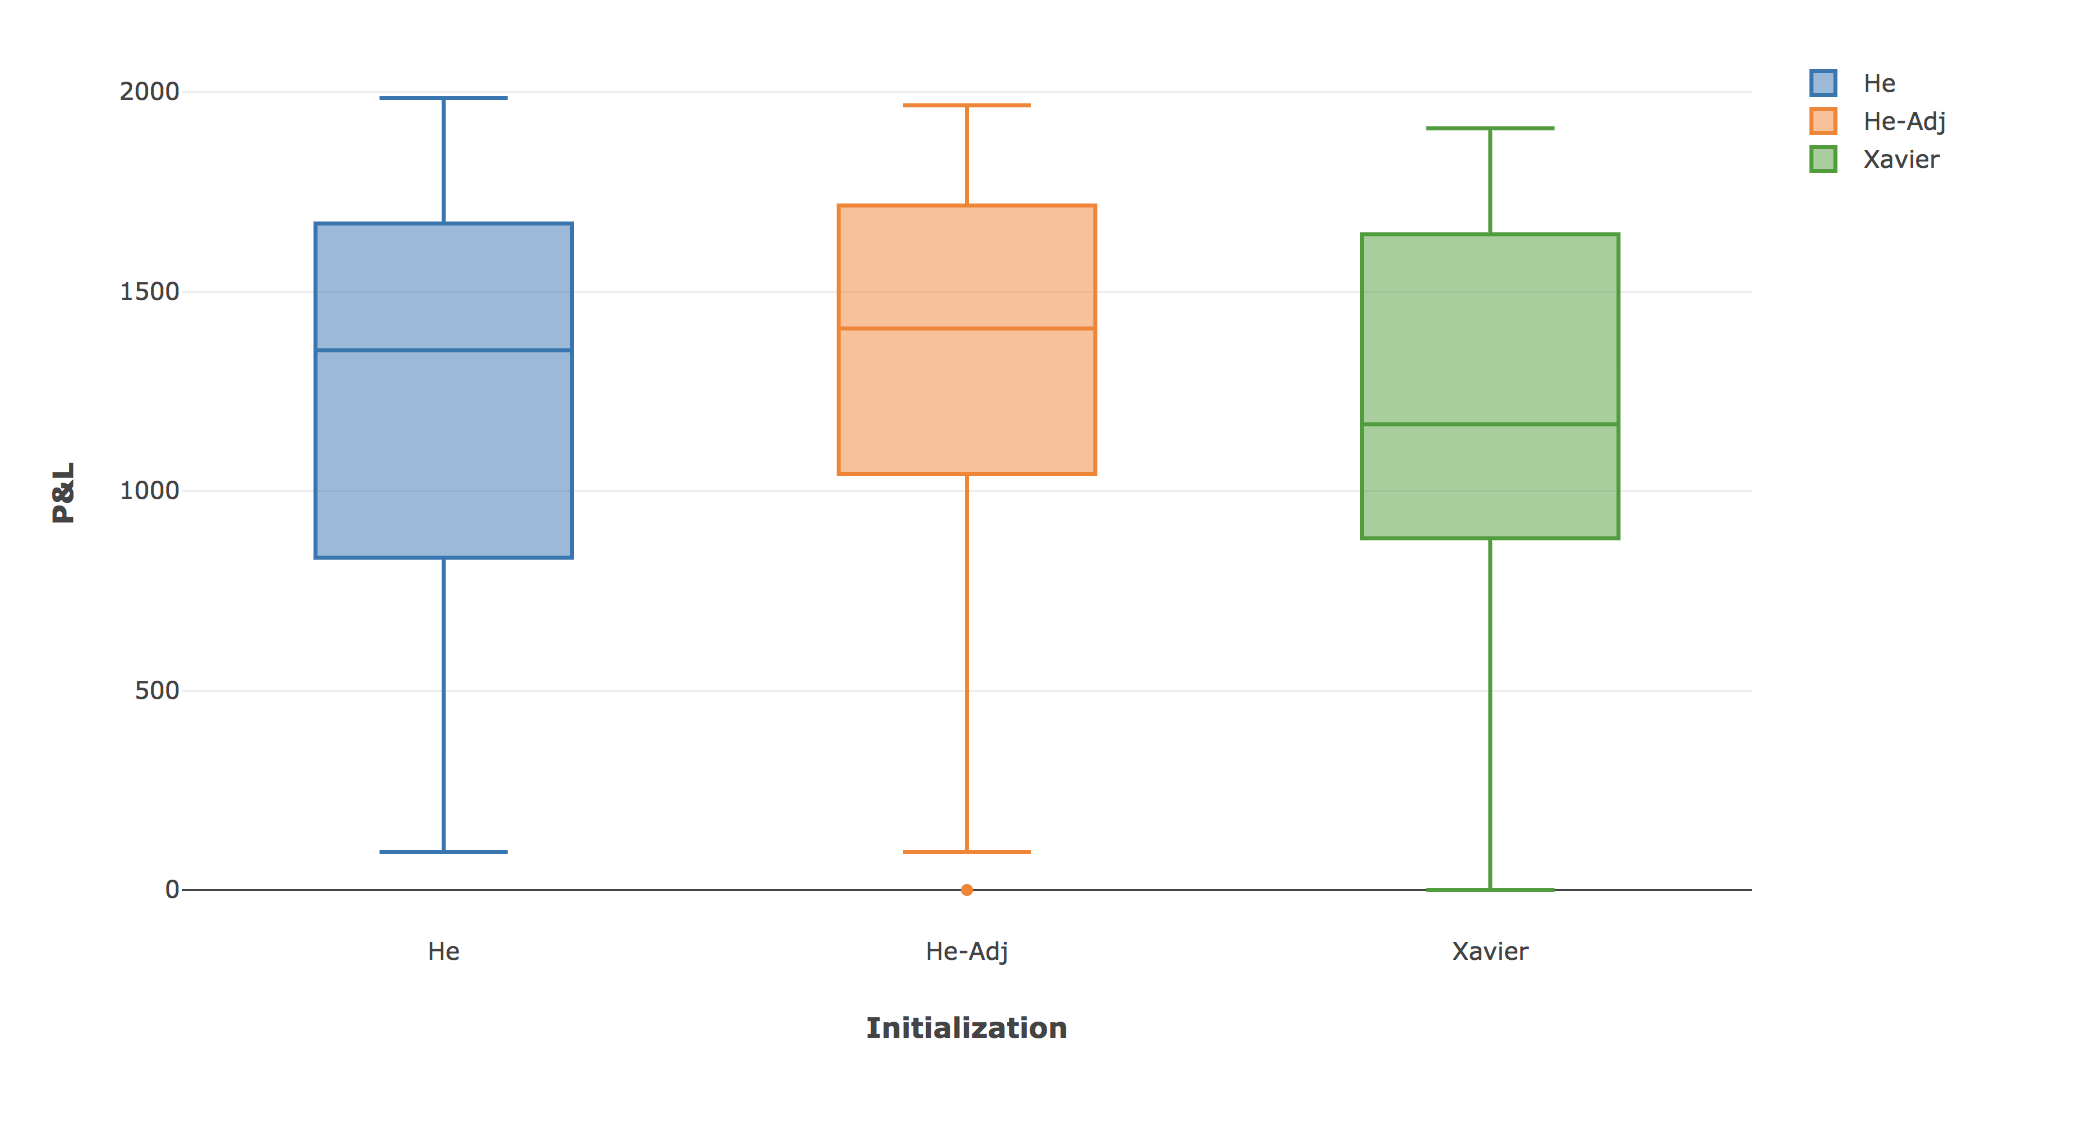
\includegraphics[scale=0.35]{images/results/init/Synthetic10_pl.png}
	%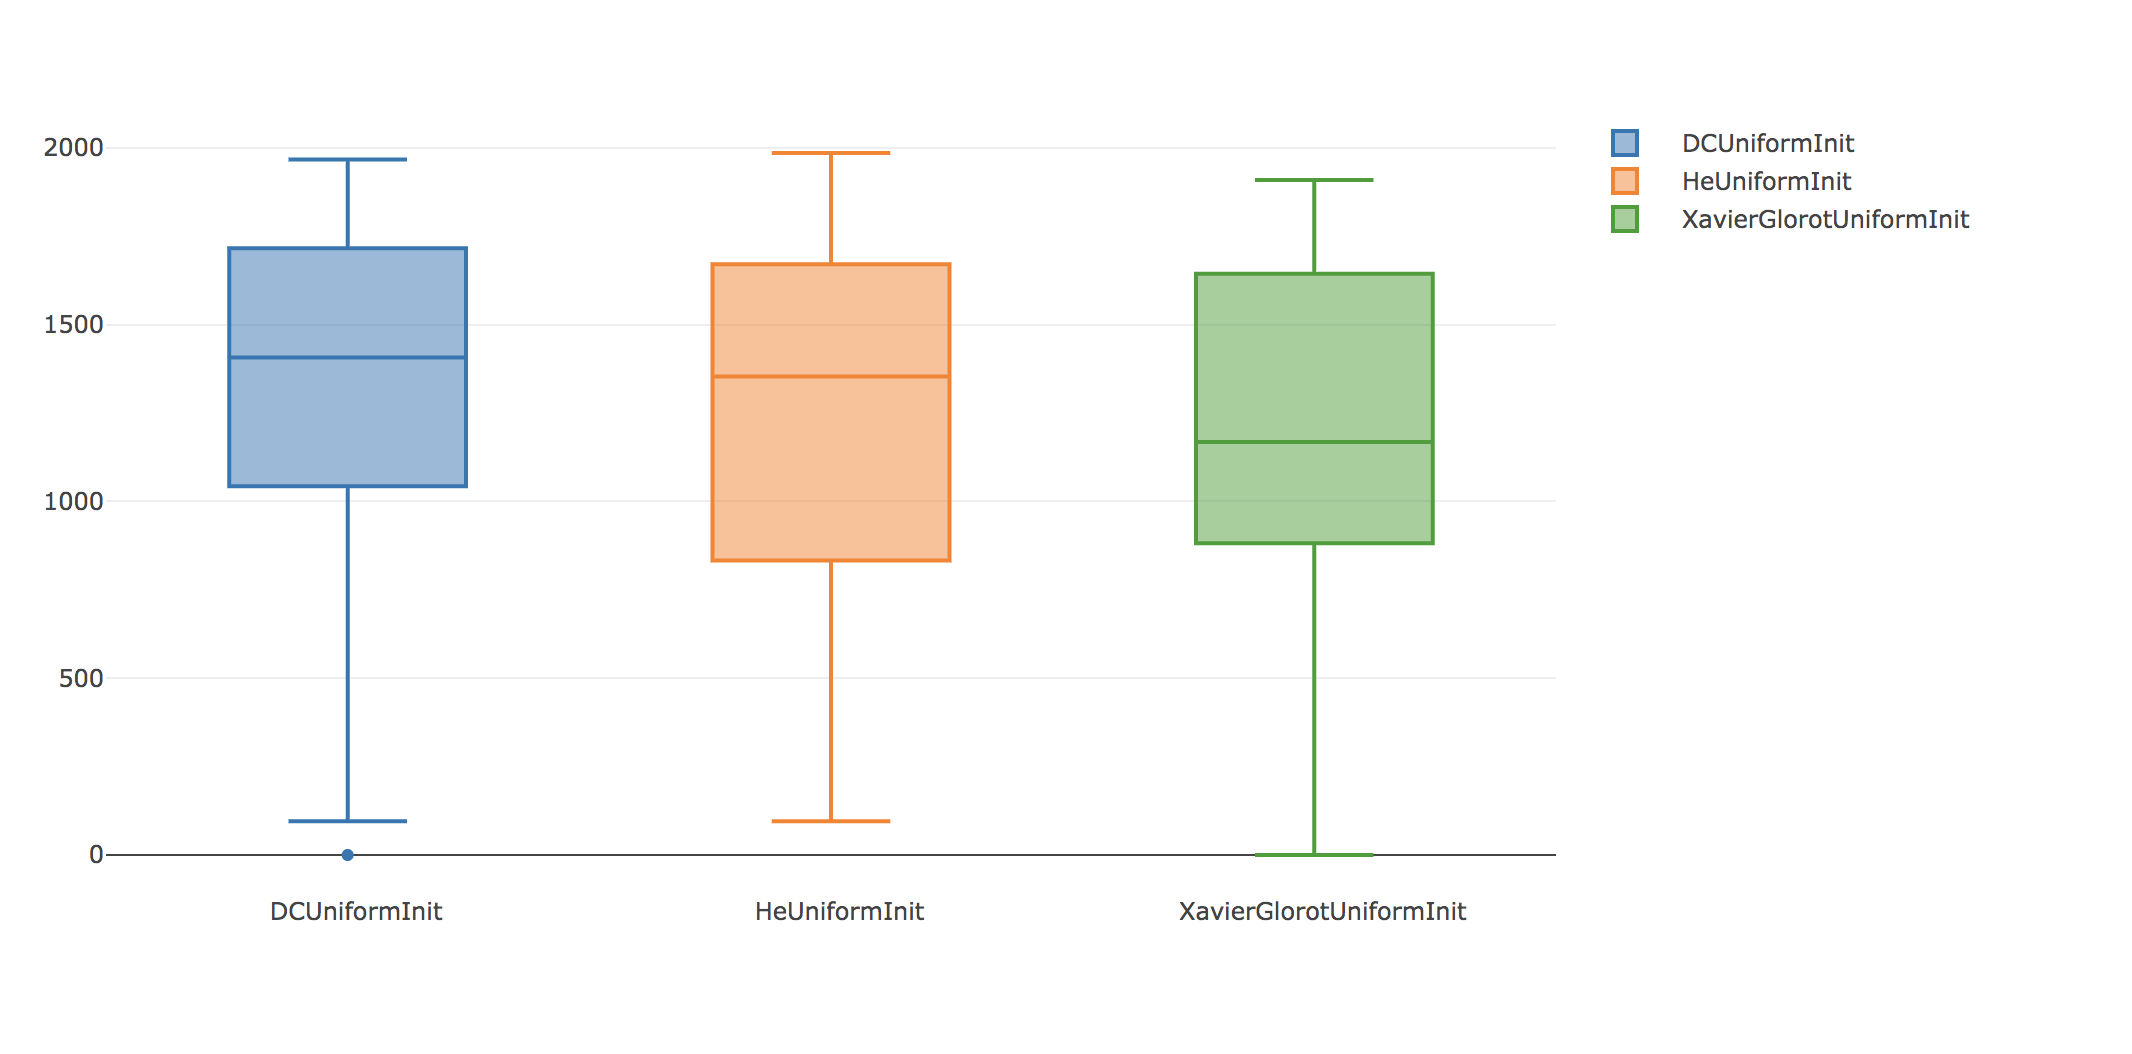
\includegraphics[scale=0.35]{images/iteration_five/init4_ffn_init.png}
	\caption{Dataset: Synthetic10 (\ref{dataset_synthetic10}); Configurations 5 and 6 (\ref{config5}, \ref{config6})
		\newline The figure here shows the P\&L performance for He-Adj and He being higher than Xavier, as to be expected with more balanced network layers and ReLU activations. The better performance in the lower end of the He-Adj and configurations when compared to He can be attributed to the inclusion of inconsistently sized layers in the configuration set, where He-Adj and would have performed better.}
	\label{figure-init4_ffn_init}
\end{figure}

\begin{figure}[H]
	\centering 
	\textbf{Weight Initialization for Predictive FFN P\&L- AGL} 
		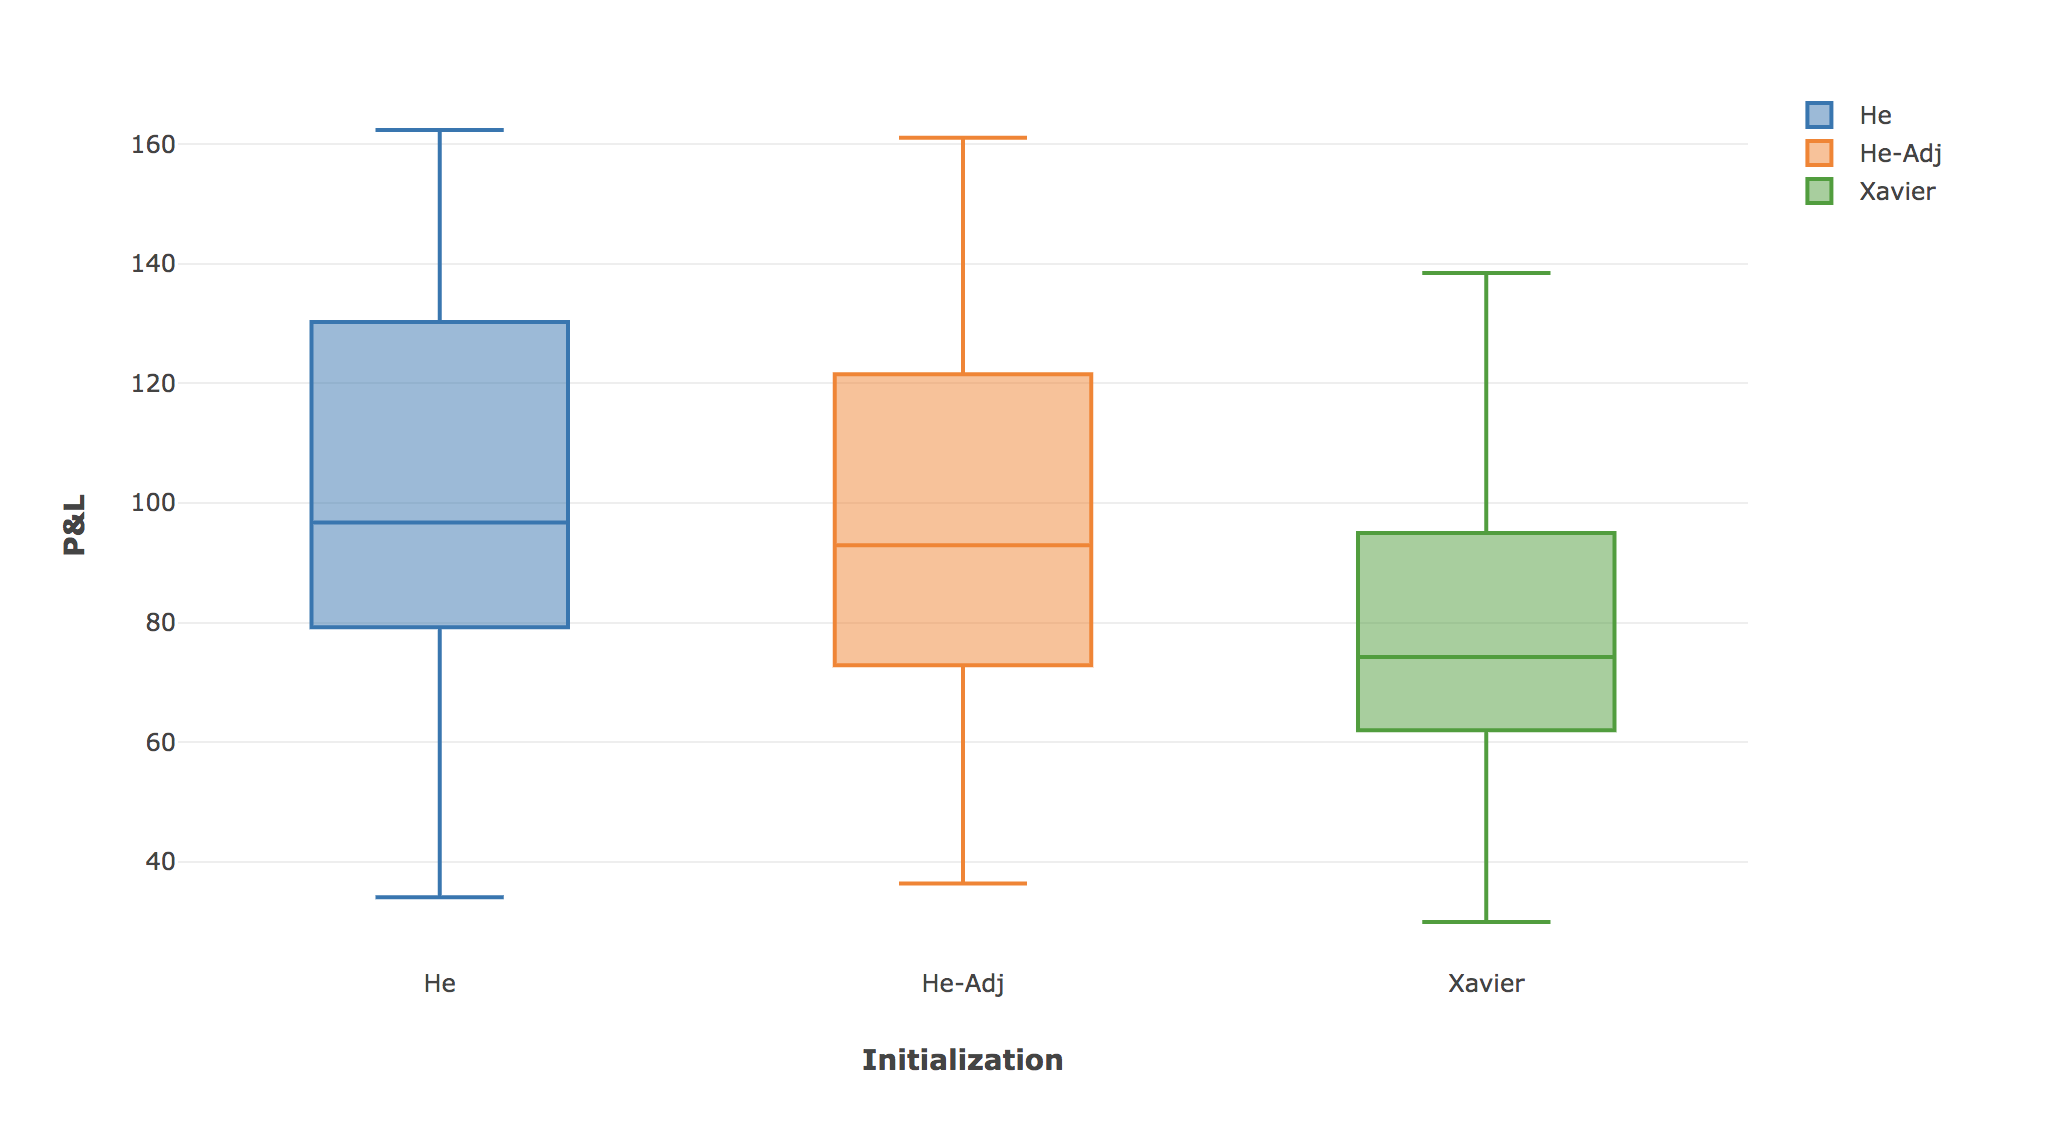
\includegraphics[scale=0.35]{images/results/init/AGL_pl.png}
	%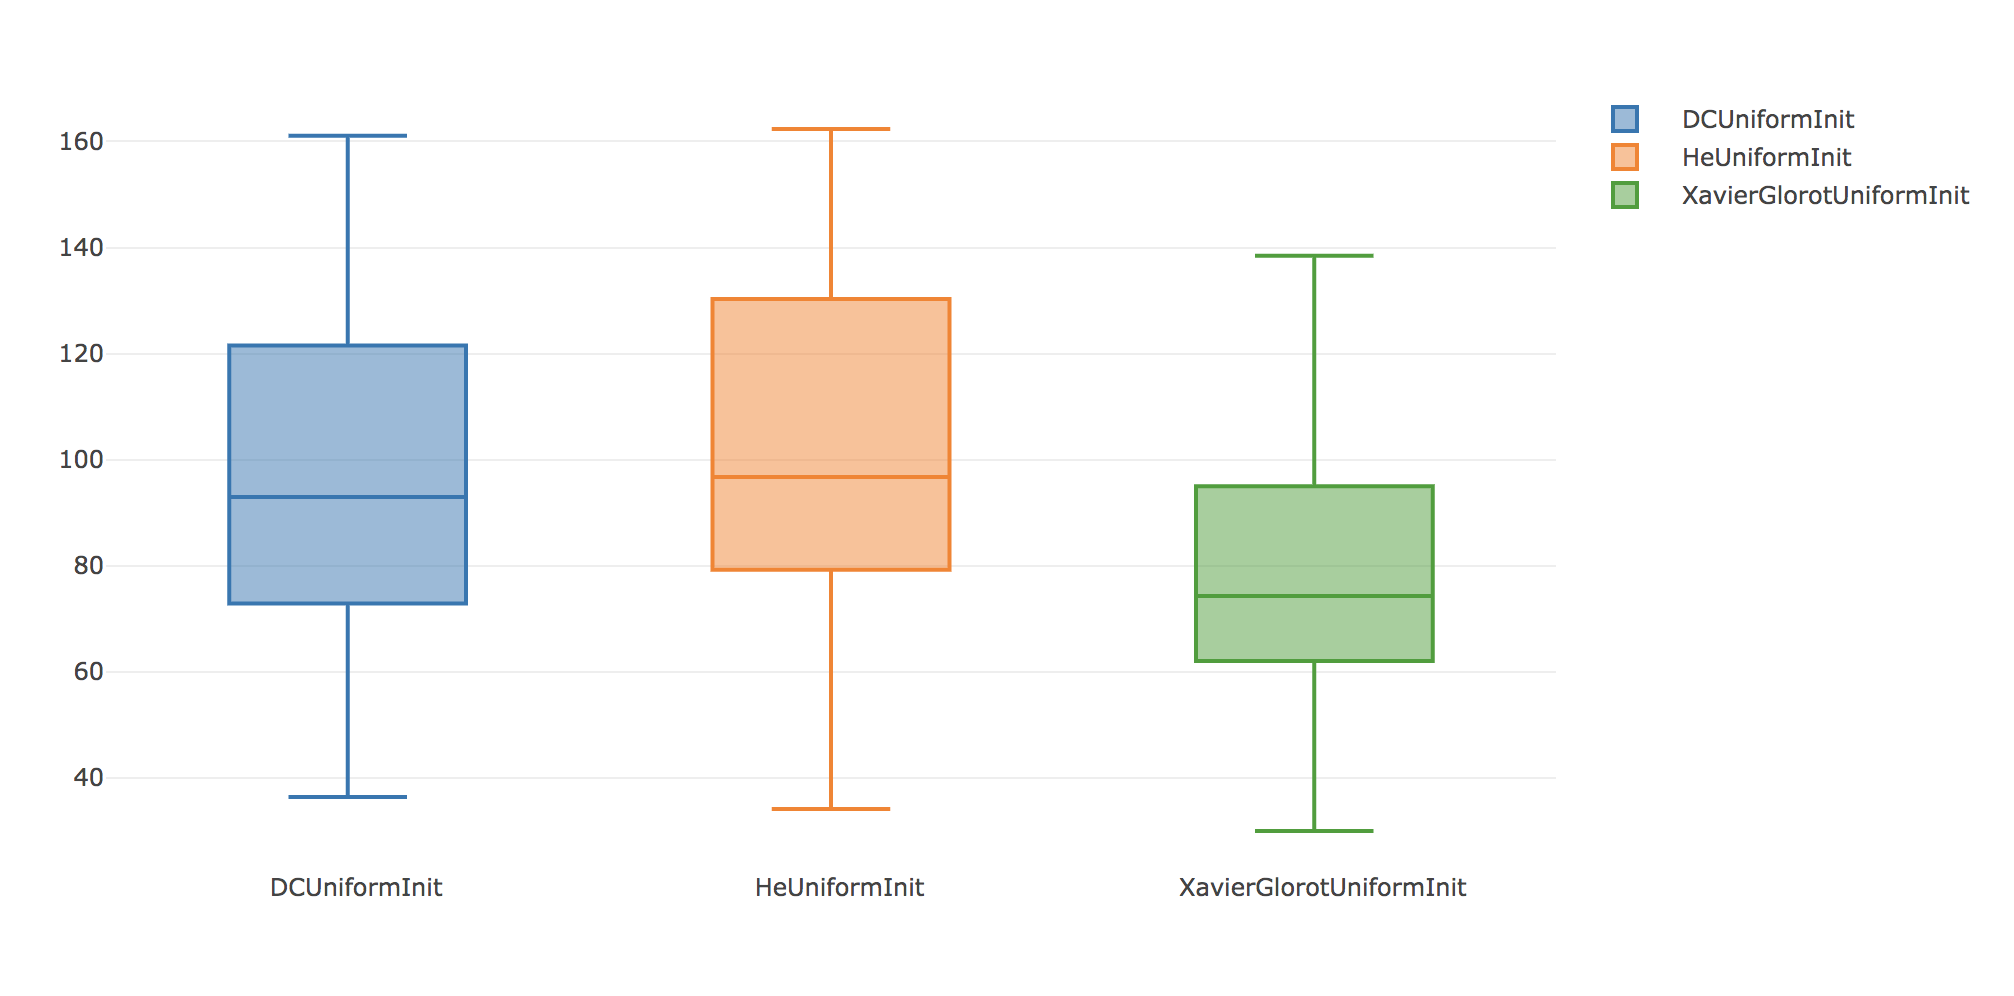
\includegraphics[scale=0.35]{images/iteration_five/init5_ffn_init.png}
	\caption{Dataset: AGL (\ref{dataset_agl}); Configuration 4 (\ref{config4})
		\newline The configurations run for AGL show notably better performance using the He-Adj and and He based initialization in comparison Xavier when using actual data, as per the differences explained above.}
	\label{figure-init5_ffn_init}
\end{figure}


\newpage
\subsection{Feature Selection}\label{results_reduction}

The figures below show the efficacy of the different feature selection sizes from the SAE and how they impact P\&L in the predictive FFN networks (i.e. the size of the SAE encoding layer). It's apparent in the results for the real data show in Figure \ref{figure-results_encoding_actual} that feature selection is occuring, with the optimal size being 10, around the degrees of freedom (or number of assets). Notably, this has the highest mean P\&L and is significantly above the '0' group which represents no encoding being performed (i.e. no SAE process prior to the predictive network). This pattern is less clear in the synthetic results shown in Figure \ref{figure-results_encoding_synthetic}, where the mean mostly trends upwards as the feature selection size increases, though the gradient of increase decreases notably after 10.\newline

\fcolorbox{red}{white}{I'm unsure of the synthetic data explanation for this}

\begin{figure}[H]
	\centering 
	\textbf{P\&L By Feature Selection Size: Actual Data}
	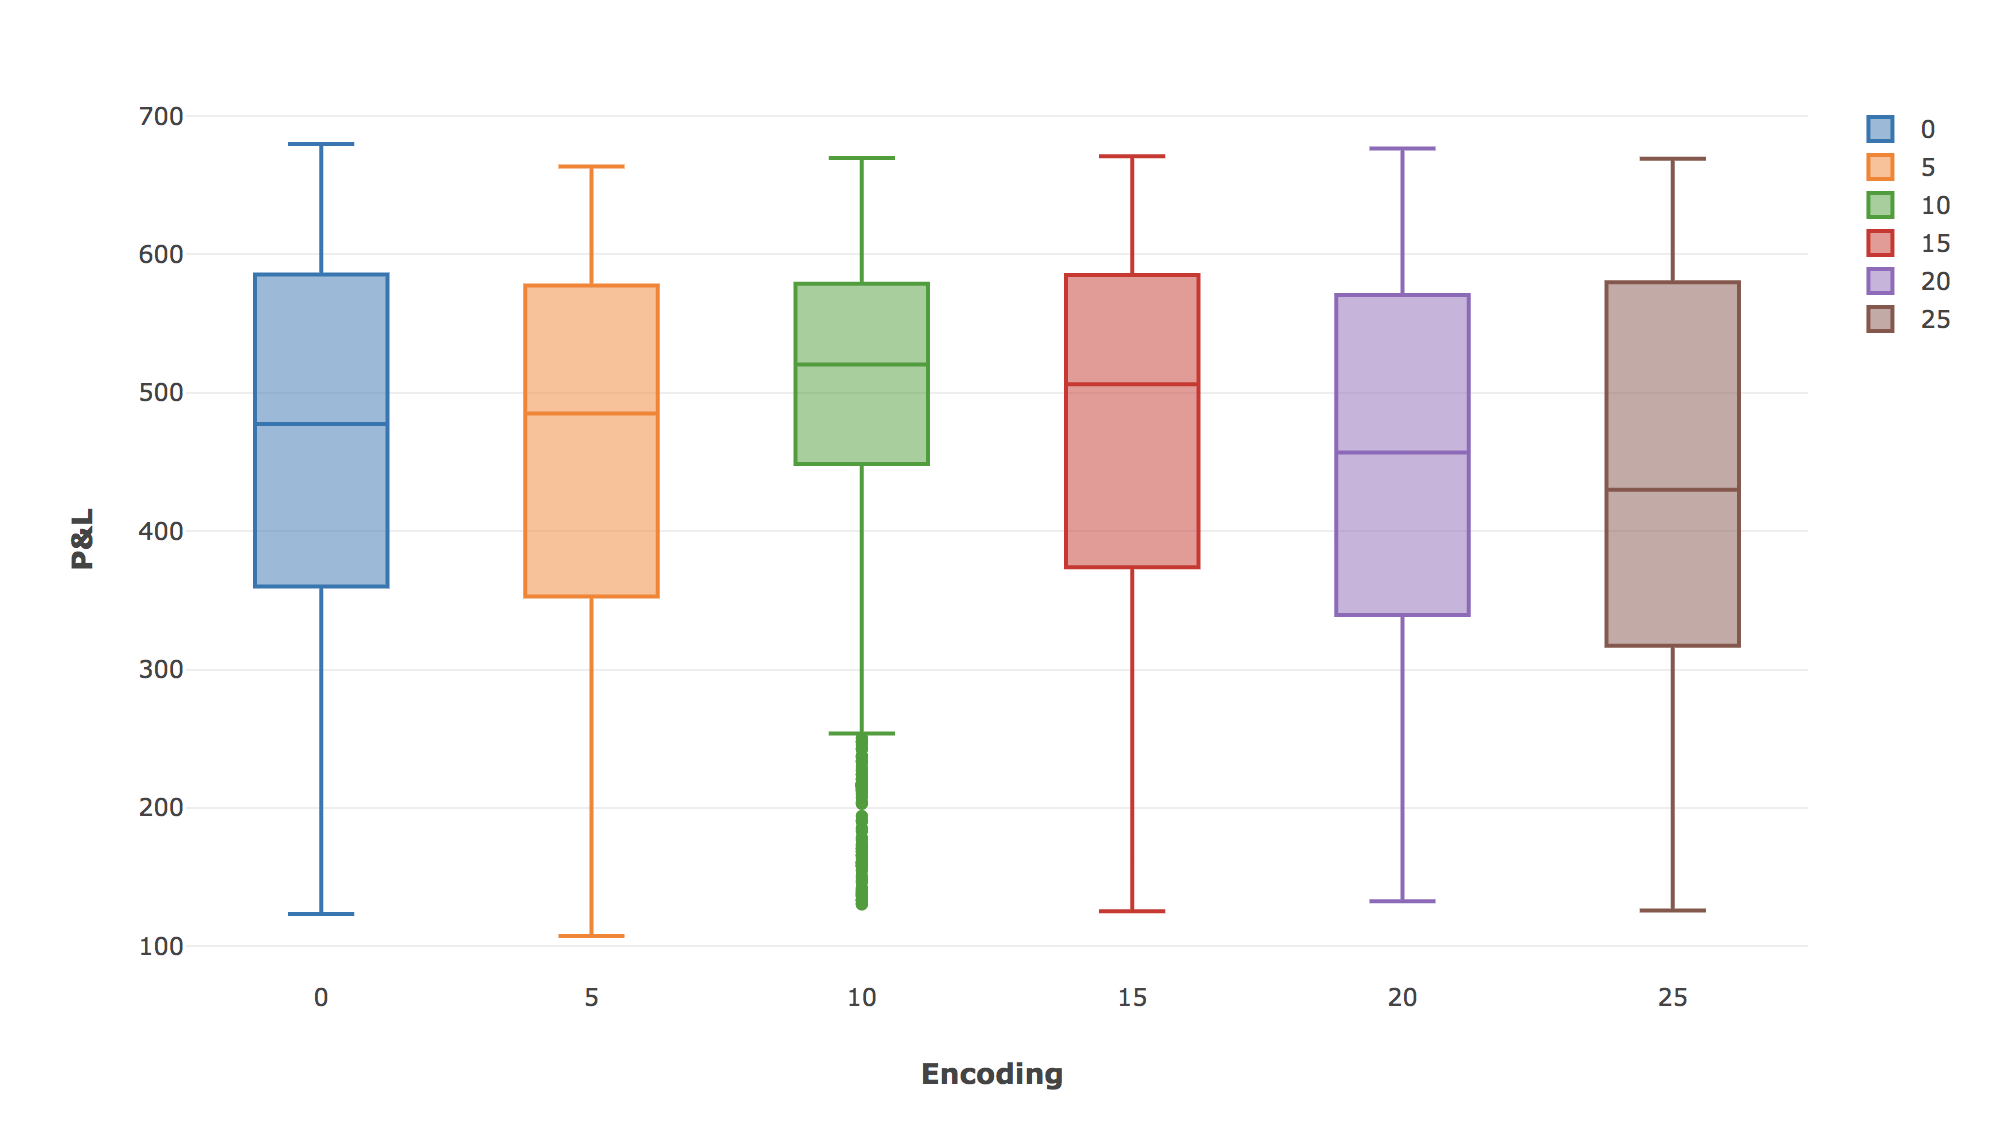
\includegraphics[scale=0.35]{images/results/feature_selection/actual_encoding_profits.png} 
	%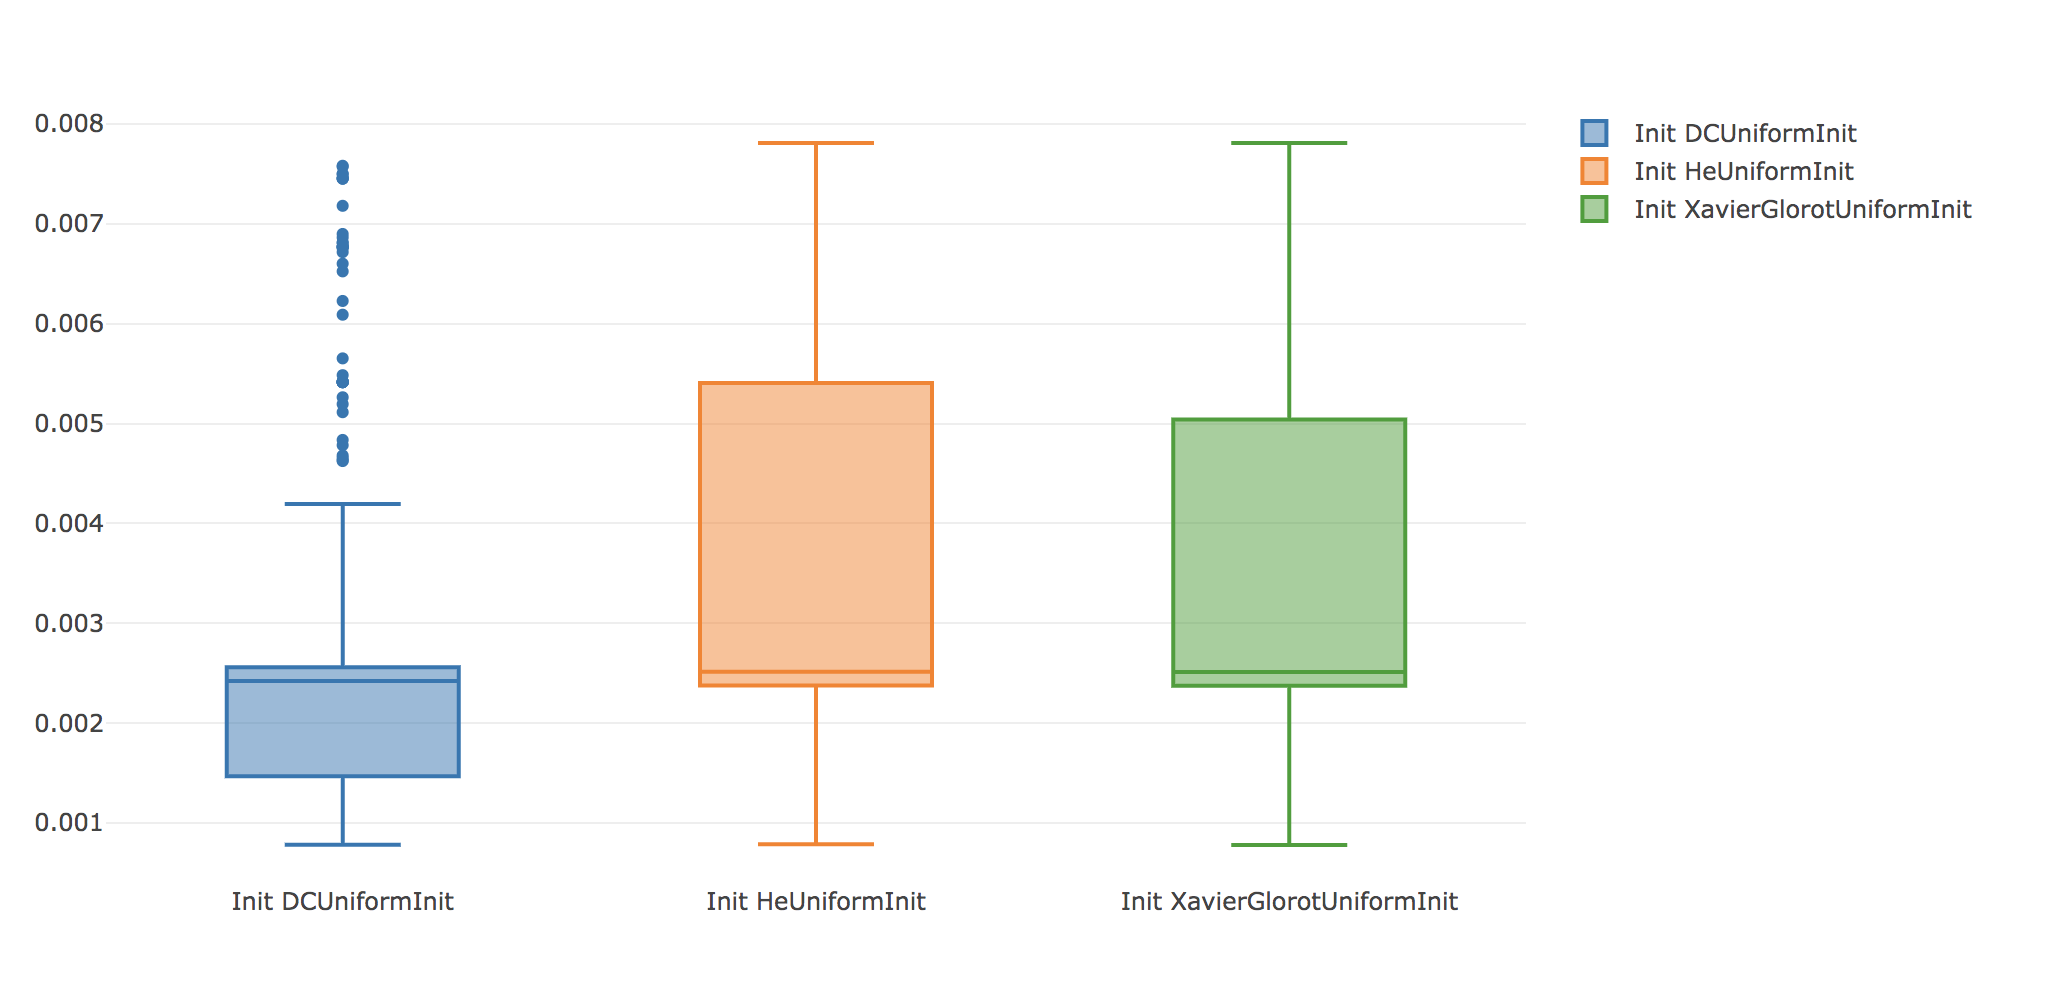
\includegraphics[scale=0.35]{images/iteration_five/it5_sae_init_agl.png}
	\caption{Dataset: ; Configuration 
		\newline Actual P\&L grouped according to feature selection size (where 0 is no encoding), showing increased performance the closer feature selection is to the number of assets (in this case, 10).}
	\label{figure-results_encoding_actual}
\end{figure}

\begin{figure}[H]
	\centering 
	\textbf{P\&L By Feature Selection Size: Synthetic Data}
	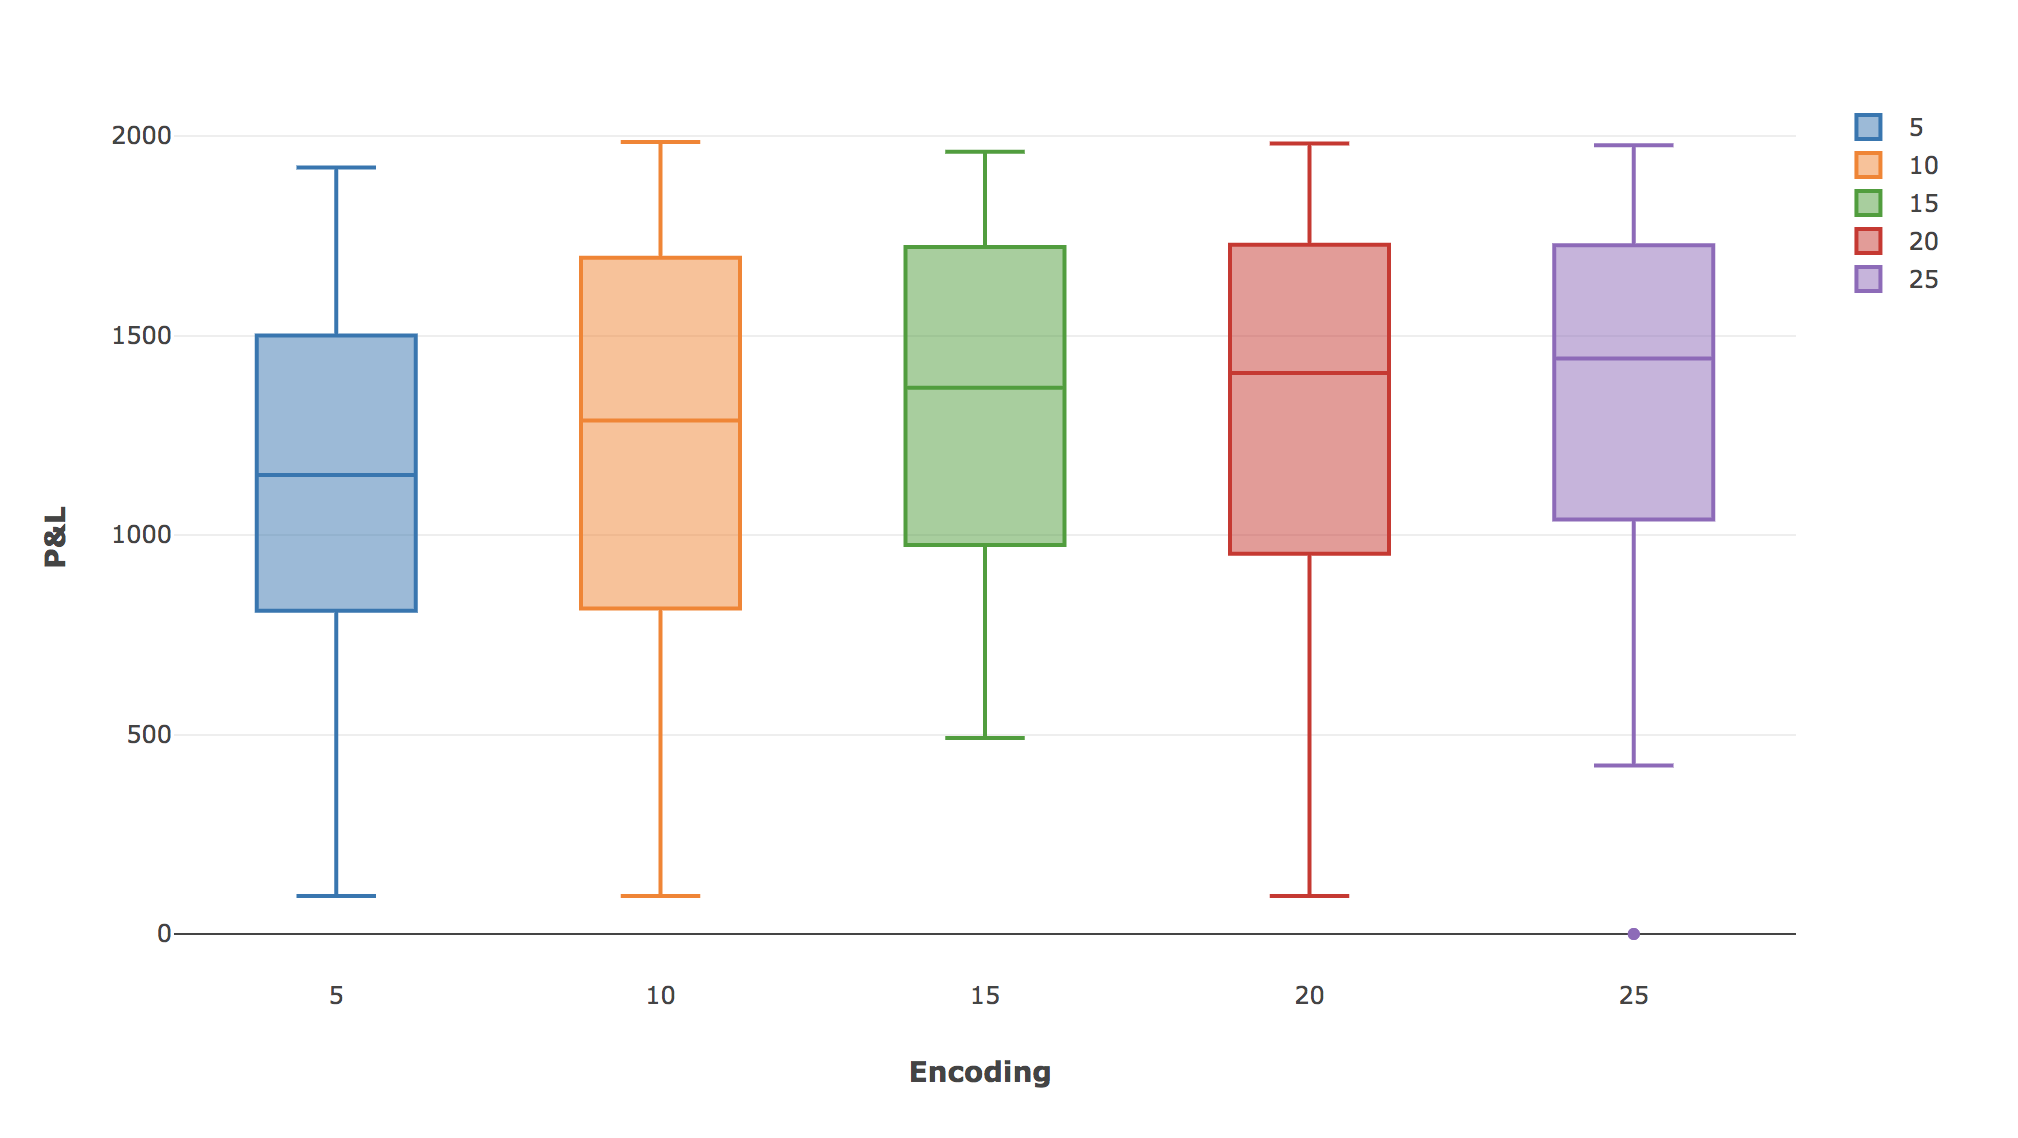
\includegraphics[scale=0.35]{images/results/feature_selection/synthetic_encoding_profits.png} 
	%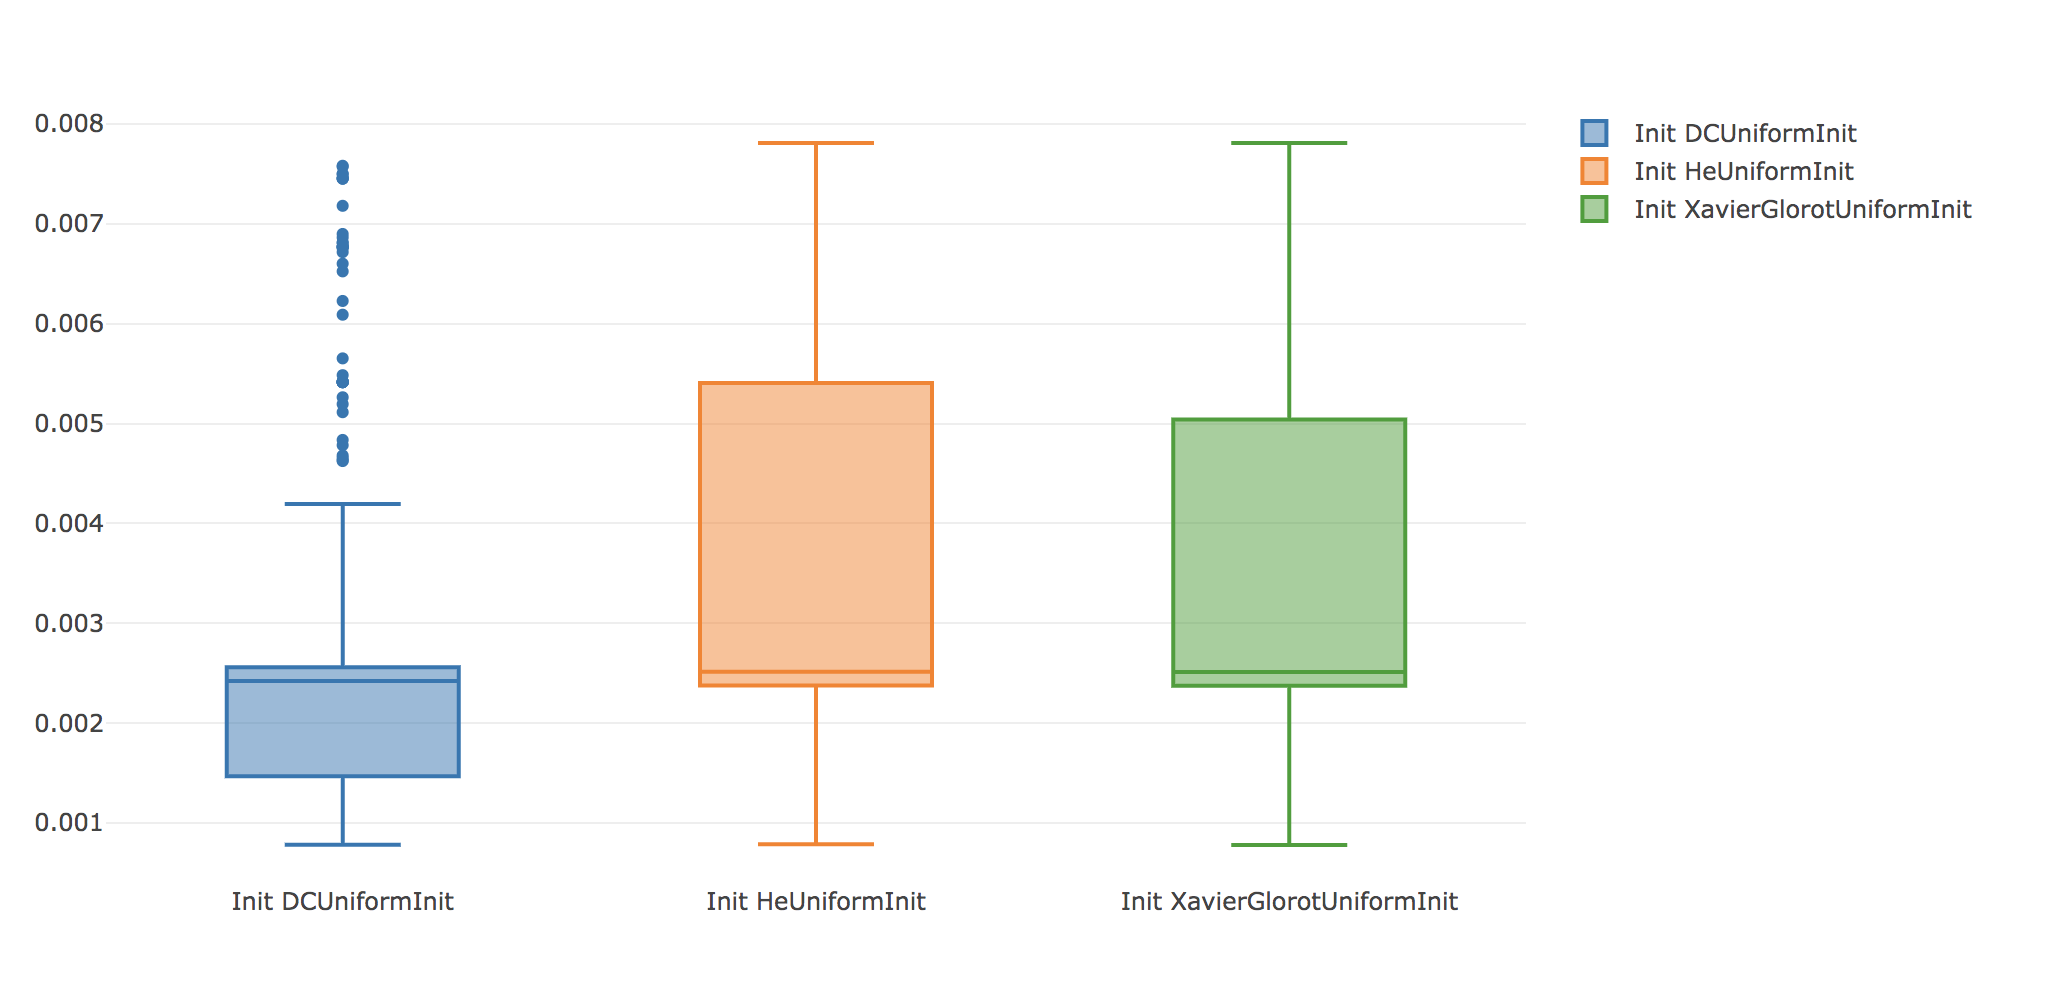
\includegraphics[scale=0.35]{images/iteration_five/it5_sae_init_agl.png}
	\caption{Dataset: Synthetic10 (\ref{dataset_synthetic10}) ; Configurations 5 \& 6 (\ref{config5}, \ref{config6})
		\newline Synthetic P\&L grouped according to feature selection size.}
	\label{figure-results_encoding_synthetic}
\end{figure}
























\newpage
\fcolorbox{red}{white}{Demarcation}
\newpage

\subsection{Network Structure and Training}\label{results_network}

\subsubsection{Effects of Network Size}

The effects of networks size on SAE MSE performance and the predictive P\&L performance are shown in Figure \ref{figure-network_size} below. The boxplots showing data for different SAE and predictive networks, for both actual and synthetic data, can be seen in the appendix (section \ref{results_network_appendix}). The trends for both actual and synthetic data were largely the same, and so only actual data has been considered here.

\begin{figure}[H]
	\centering
	\textbf{Network Performance by Size}
	\begin{subfigure}{.5\textwidth}
		\centering 
		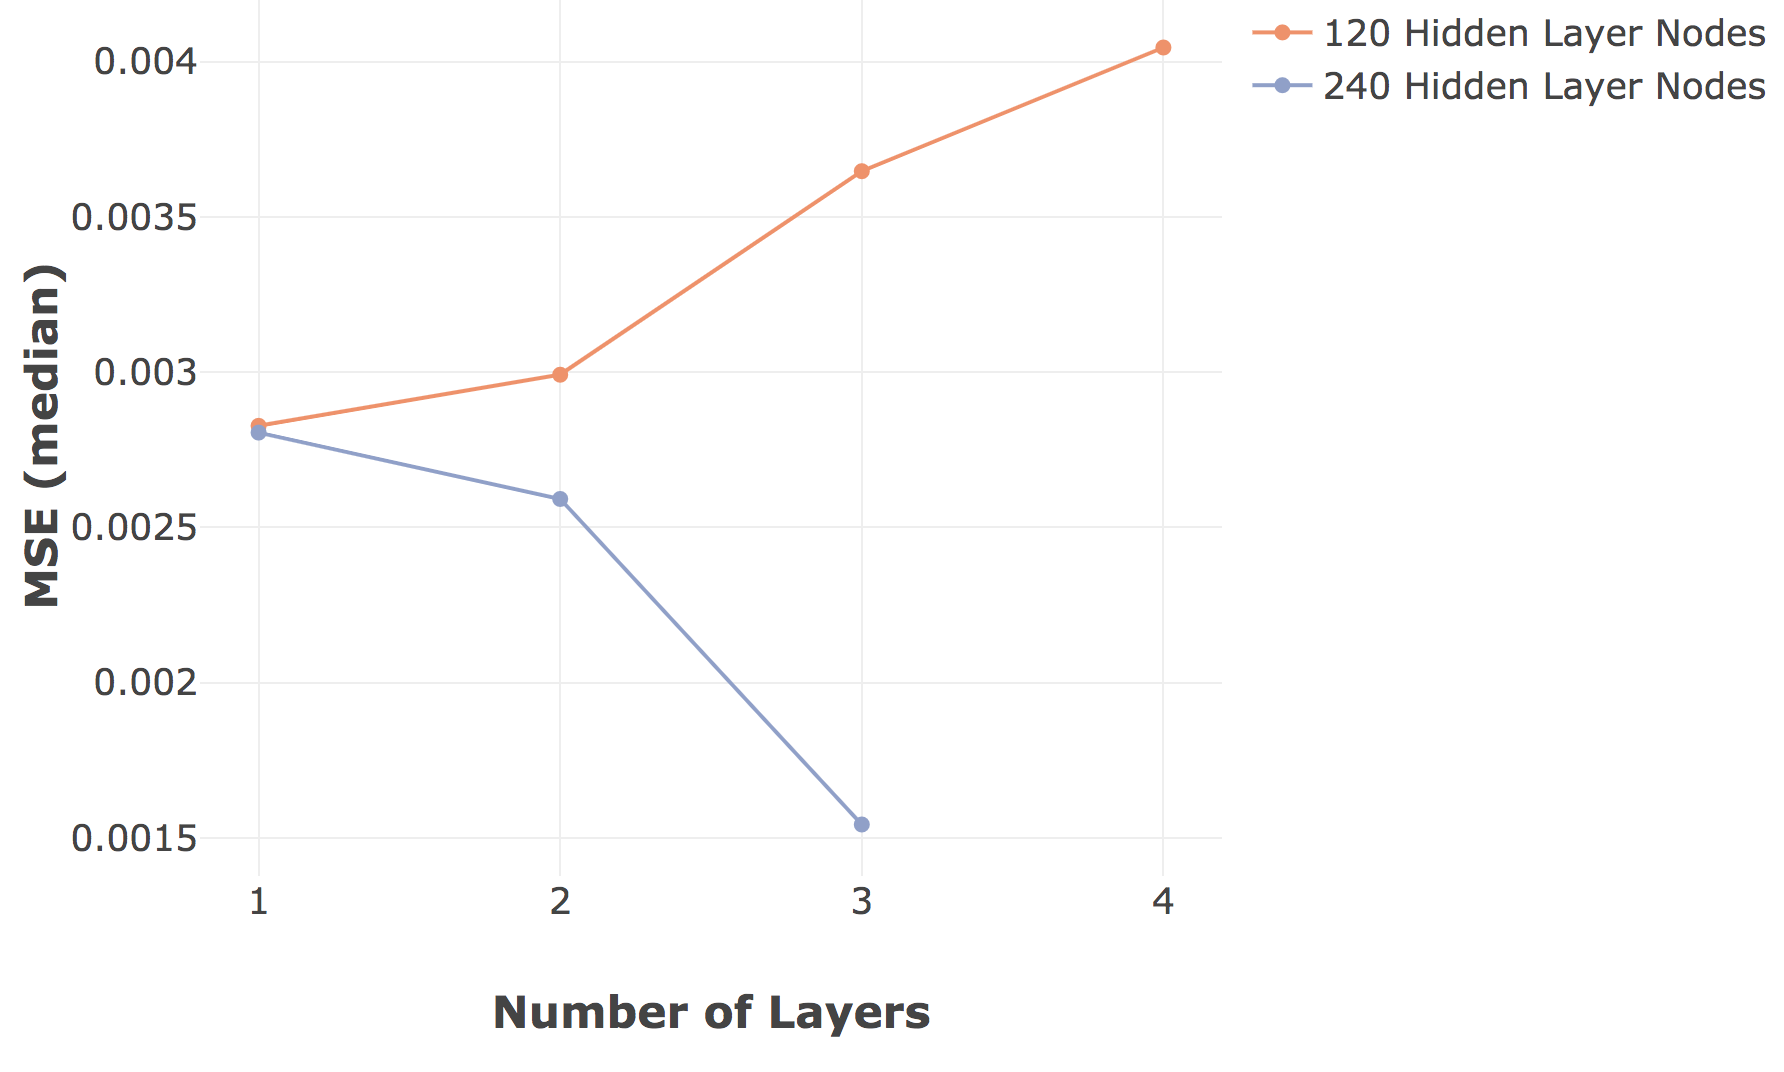
\includegraphics[scale=0.25]{images/results/network/actual_mse_lines.png}
		\caption{\textbf{SAE MSE Scores} 
			\newline }
		\label{figure-actual_mse_lines}
	\end{subfigure}%
	\begin{subfigure}{.5\textwidth}
		\centering 
		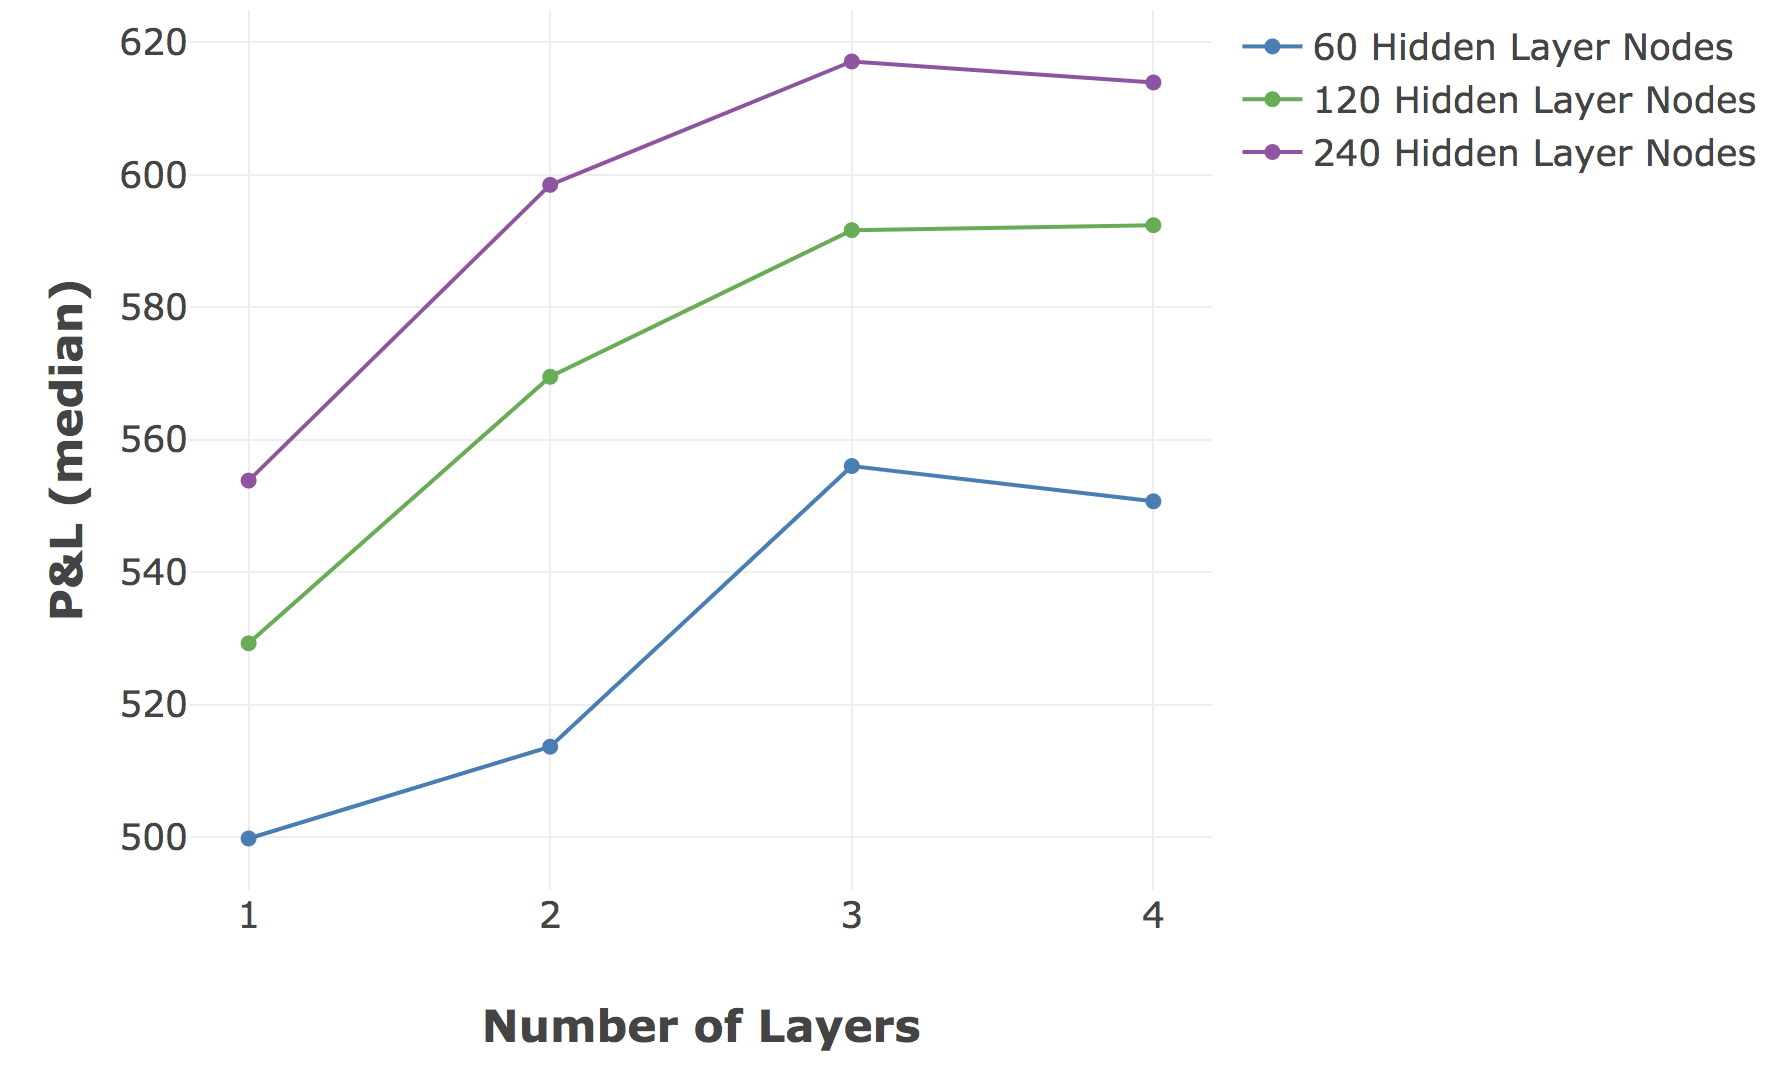
\includegraphics[scale=0.26]{images/results/network/actual_pl_lines.png}
		\caption{\textbf{Predictive P\&L Scores} 
			\newline }
		\label{figure-actual_pl_lines}
	\end{subfigure}
	\caption{Dataset: Actual10 dataset (\ref{dataset_actual10}), Configuration 
		\newline Figure (a) shows the median minimum MSE by SAE networks achieved with the indicated number of layers and layer nodes. It's worth noting that the number of layers here indicate the final SAE structure of $N$ hidden layers, rather than the training structure of $2N + 1$ hidden layers. Interestingly, the networks with 120 node layers seem to struggled with training, performance decreases as layers increased. This is to be expected if the learning parameters (e.g. SGD  learning rate) are not ideal for the structure, the effects of which are amplified as network sizes increase. This is resolved in the larger 240 node networks which show significant improvement as more layers are added (as one would generally expect, subject to effective SGD).
		\newline Figure (b) shows the median OOS P\&L achieved by predictive networks with the indicated number of layers and layer nodes. The behaviour is as expected here, where network performance generally increases with size. The exception is the four layer network of 60 nodes, where the training parameters were no longer effective in passing signal back (larger layer sizes are less likely to suffer from this, particuarly with ReLU activations).
	}
	\label{figure-network_size}
\end{figure}

\paragraph{SAE Network Structures}

It was interesting to note that the typically accepted SAE network structure, where layers decrease in size between the input layer and the encoding layer, resulted in worse performance when compared to the same number of layers with constant numbers of nodes. As detailed in section \ref{results_init}, the RBM based greedy layerwise pre-training proved to be ineffective, and so weight initialization with SGD training on the entire network was used instead. It is possible that a greedy layerwise training using these methods (rather than RBM initialization) may have shown increased performance in the decreasing layer size structure, but for SGD training it was clear that larger layers at all stages increased performance. The box plots showing these trends can be seen for actual and synthetic data in the appendix, section \ref{results_network_appendix}.



\subsubsection{Effects of Learning Rates and Schedules}\label{results_lr}

Learning rate schedules were implemented such that the learning rate would rise and fall through a set of values during a set number of epochs (or epoch cycle), as discussed in \ref{imp_learning_rate_schedule}.	Conceptually, this should allow a more effective traversal of the solution space, where larger learning rates are able to dislodge the configuration from saddle points, and smaller learning rates are able to optimize at a minima. \newline


\begin{figure}[H]
	\centering
	\textbf{SAE MSE by Learning Rates}
	\begin{subfigure}{.5\textwidth}
		\centering 
		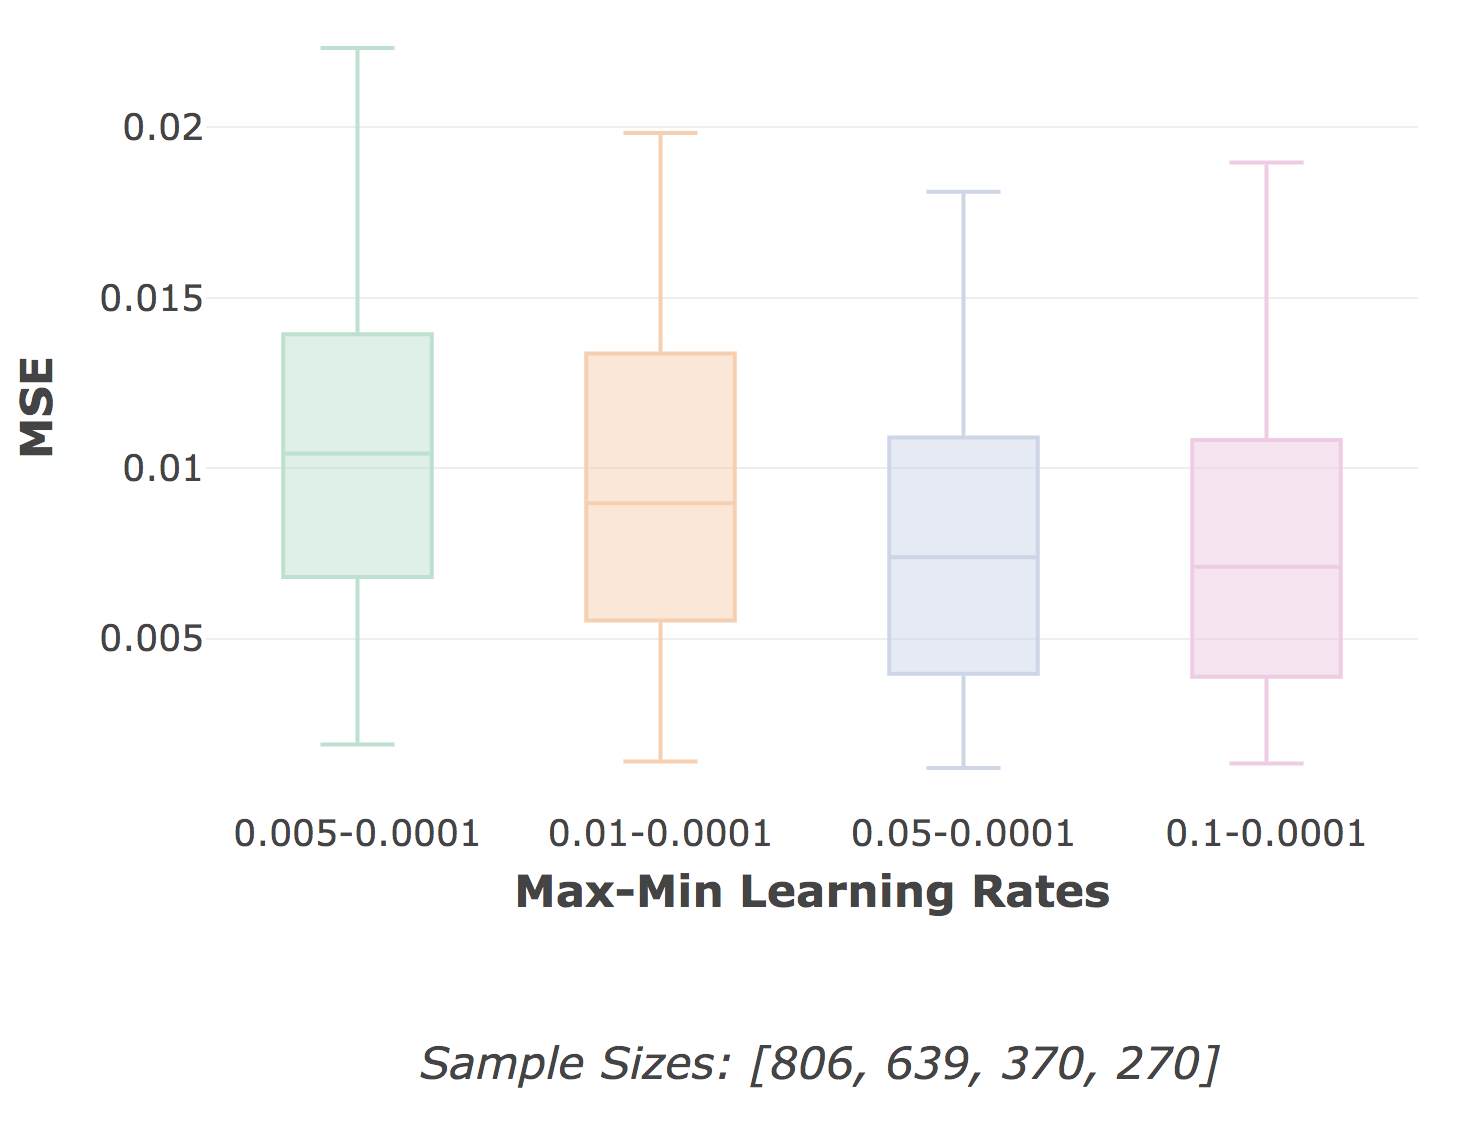
\includegraphics[scale=0.25]{images/results/network/lr/synth_mse_minmax_lr.png}
		\caption{\textbf{Synthetic Data} 
			\newline }
		\label{figure-synth_mse_minmax_lr}
	\end{subfigure}%
	\begin{subfigure}{.5\textwidth}
		\centering 
		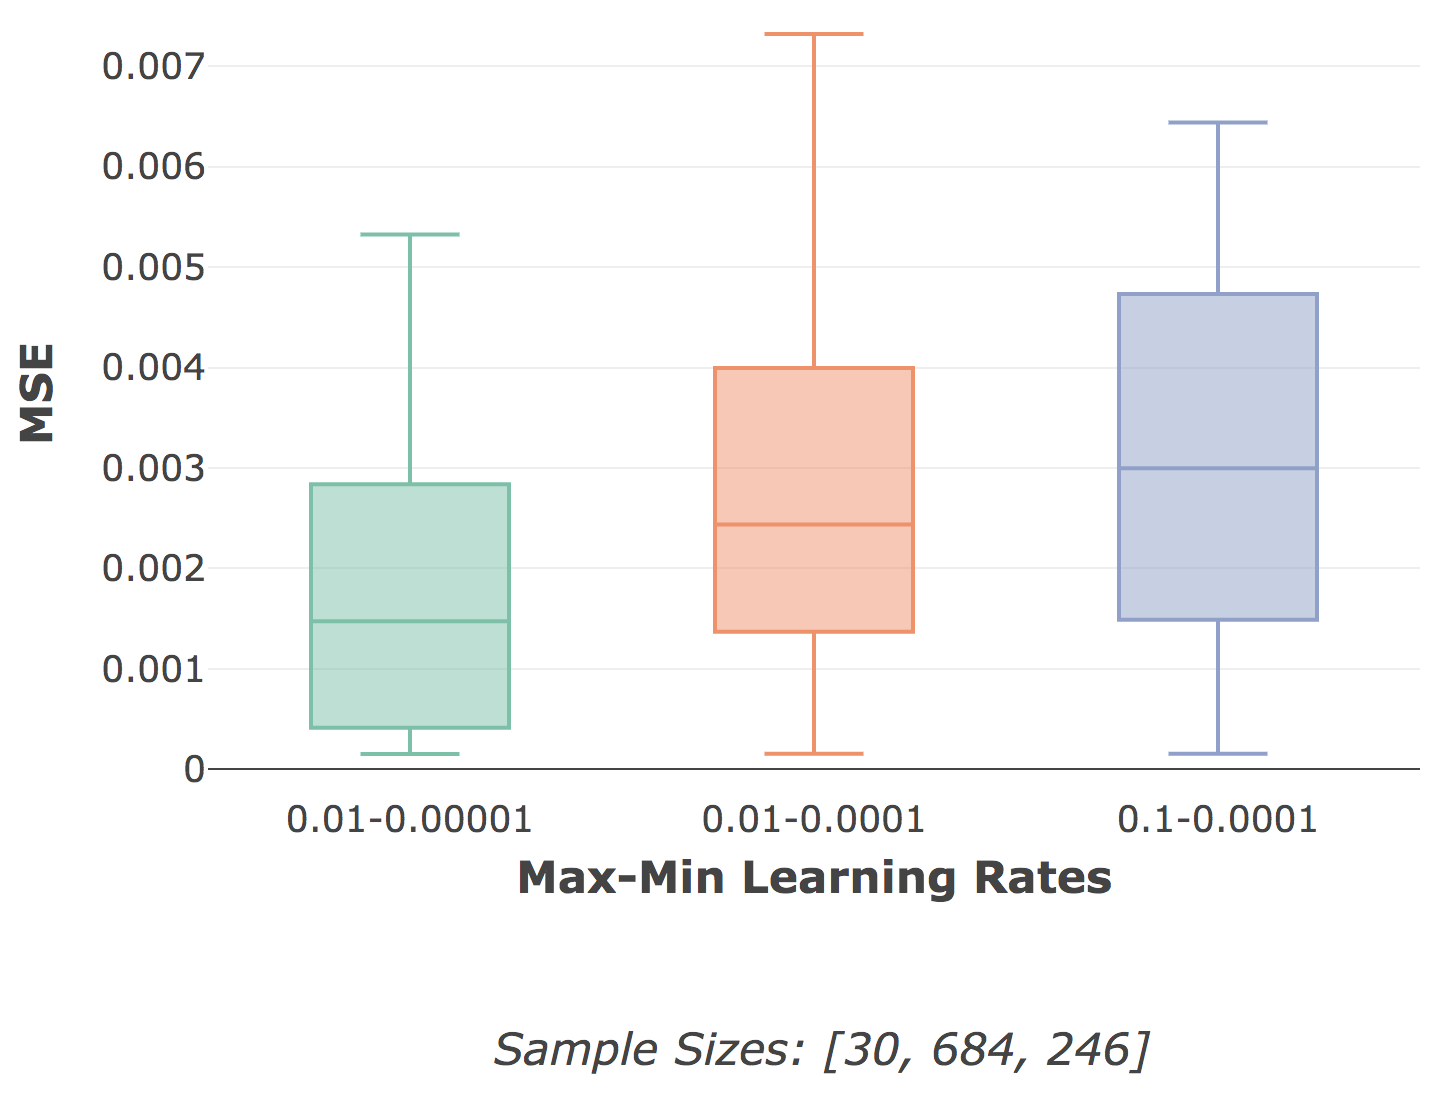
\includegraphics[scale=0.25]{images/results/network/lr/actual_mse_minmax_lr.png}
		\caption{\textbf{Actual Data} 
			\newline }
		\label{figure-actual_mse_minmax_lr}
	\end{subfigure}
	\caption{Dataset: Synthetic10 dataset (\ref{dataset_synthetic10}), Actual10 dataset (\ref{dataset_actual10}), Configuration
		\newline It is interesting to  note that the effects here are quite different for Synthetic and Actual data, with networks for Synthetic data favouring learning rate ranges with a higher upper bound, and Actual data networks trending in favour of lower upper bound ranges. The synthetic data is structurally less complex, as discussed further in \ref{results_gbm_data} and \ref{results_data_hist}, and so the larger learning rates will allow for quicker optimisation. Conversely, SAE networks for actual data benefit from a more careful exploration of the solution space.}
	\label{figure-mse_lr}
\end{figure}


\begin{figure}[H]
	\centering
	\textbf{P\&L by Learning Rates}
	\begin{subfigure}{.5\textwidth}
		\centering 
		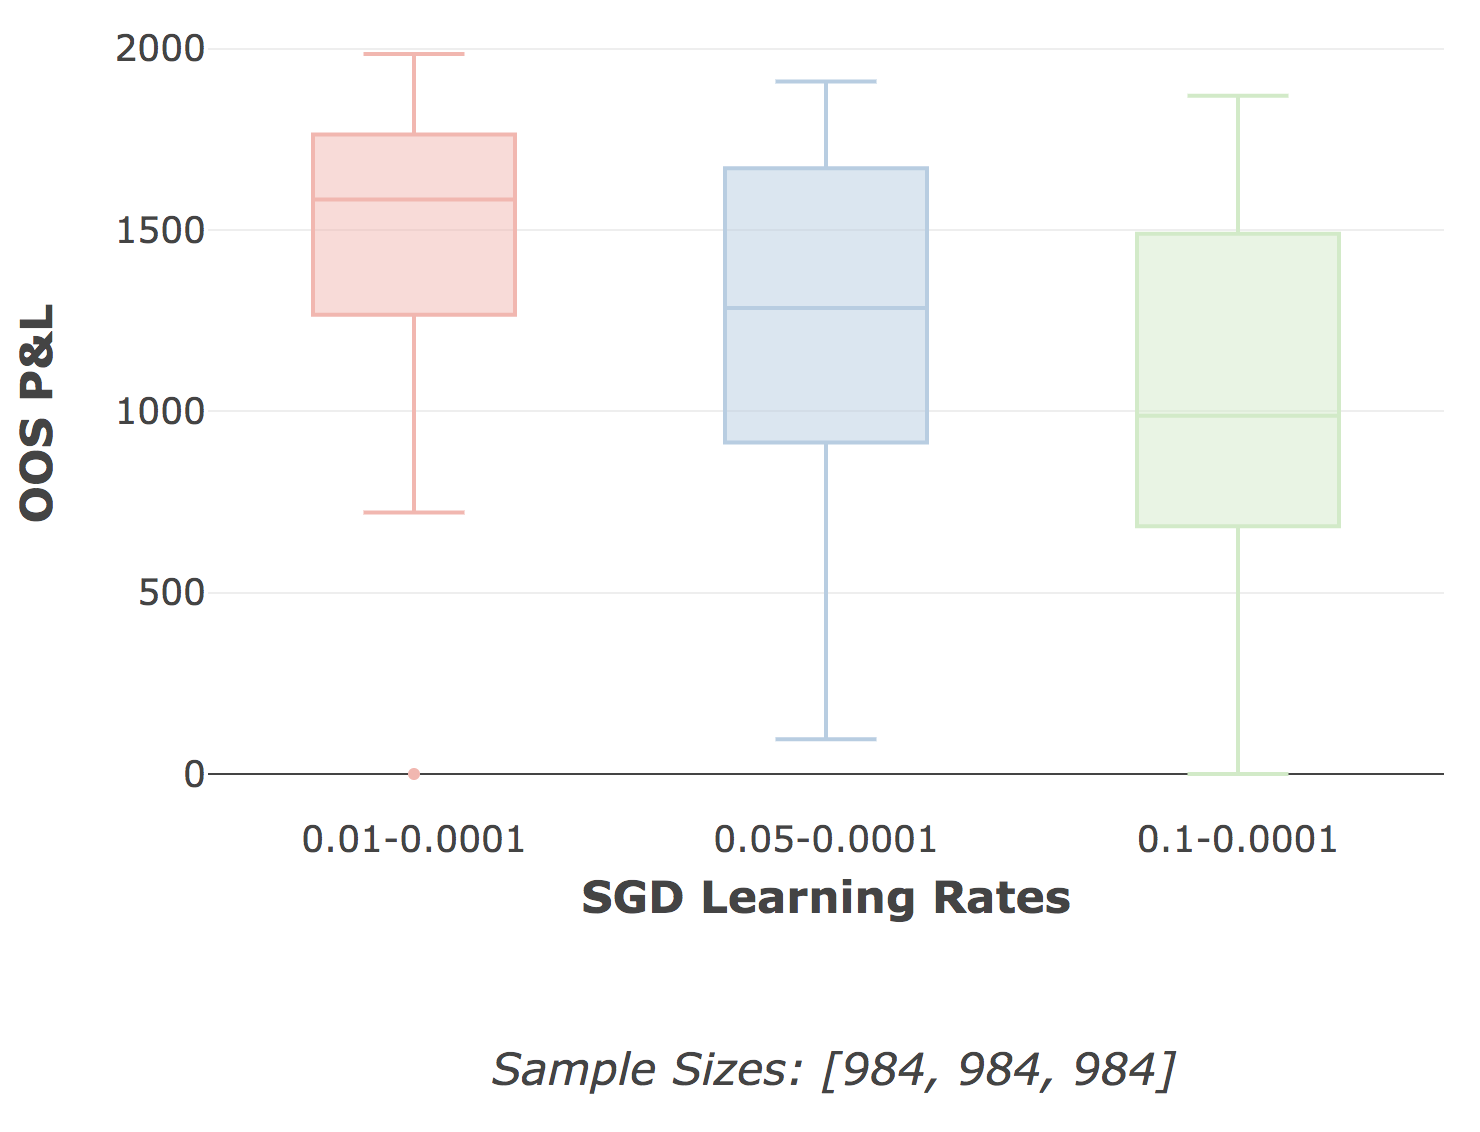
\includegraphics[scale=0.25]{images/results/network/lr/synth_pl_minmax_lr.png}
		\caption{\textbf{Synthetic Data} 
			\newline }
		\label{figure-synth_pl_minmax_lr}
	\end{subfigure}%
	\begin{subfigure}{.5\textwidth}
		\centering 
		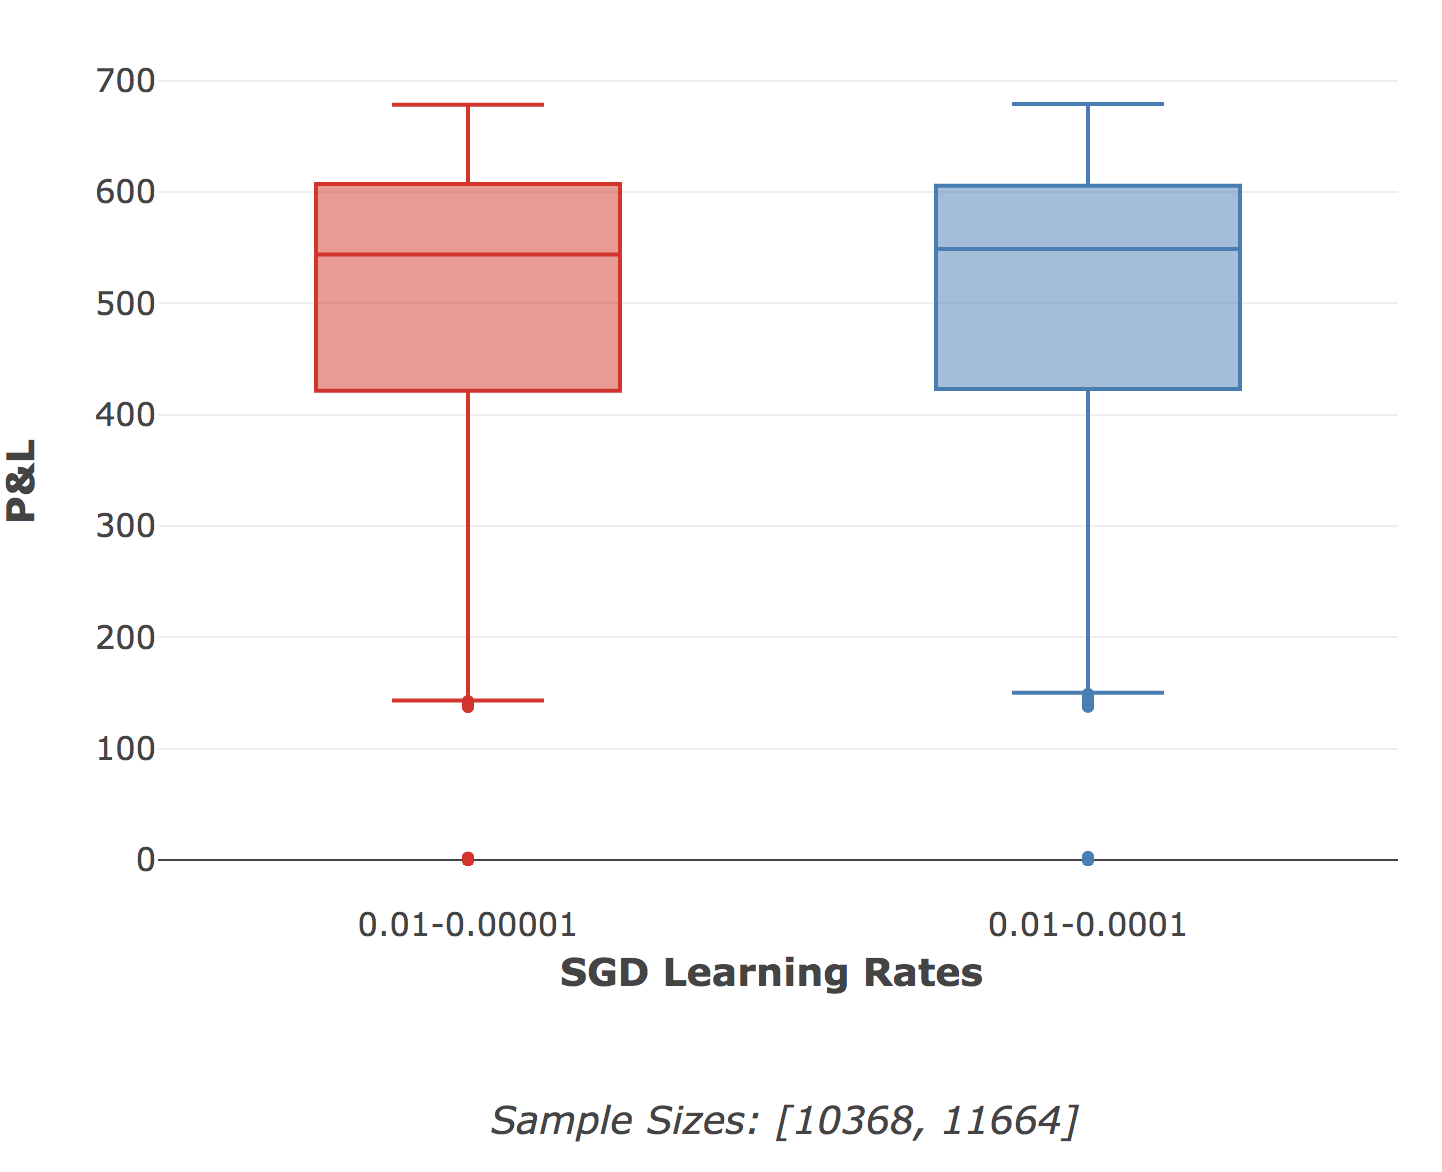
\includegraphics[scale=0.25]{images/results/network/lr/actual_pl_minmax_lr.png}
		\caption{\textbf{Actual Data} 
			\newline }
		\label{figure-actual_pl_minmax_lr}
	\end{subfigure}
	\caption{Dataset: Synthetic10 dataset (\ref{dataset_synthetic10}), Actual10 dataset (\ref{dataset_actual10}), Configuration
		\newline The learning rates for Actual data showin in Figure (b) here were chosen accordingly to the best rates seen in the SAE training. There's no substantial difference shown by changing the lower bound by a factor. The results for Synthetic data were interesting in that the networks had higher P\&L when trainined with ssmaller learning rates, suggesting that the predictive task still warrants a more careful solution space exploration despite the less complex nature of the data.}
	\label{figure-pl_lr}
\end{figure}

\begin{figure}[H]
	\centering
	\textbf{Effects of Epoch Cycle Lengths (Actual Data)}
	\begin{subfigure}{.5\textwidth}
		\centering 
		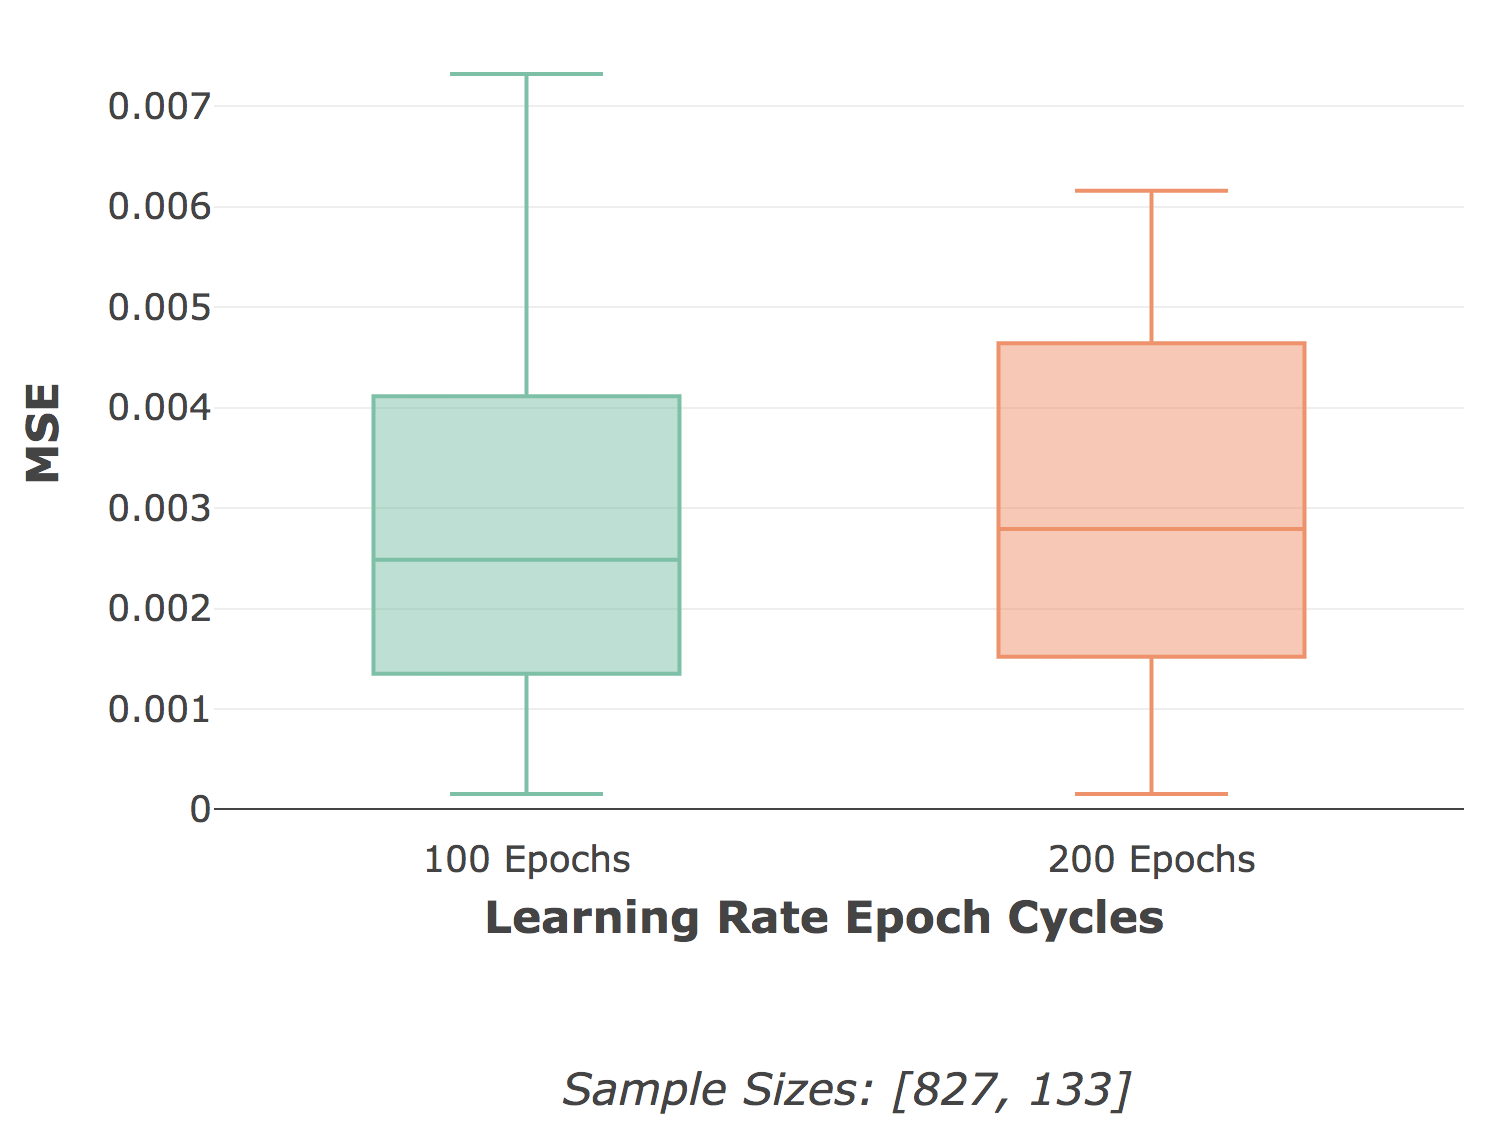
\includegraphics[scale=0.26]{images/results/network/lr/actual_mse_lr_epochs.png}
		\caption{\textbf{MSE for SAE Networks} 
			\newline }
		\label{figure-actual_mse_lr_epochs}
	\end{subfigure}%
	\begin{subfigure}{.5\textwidth}
		\centering 
		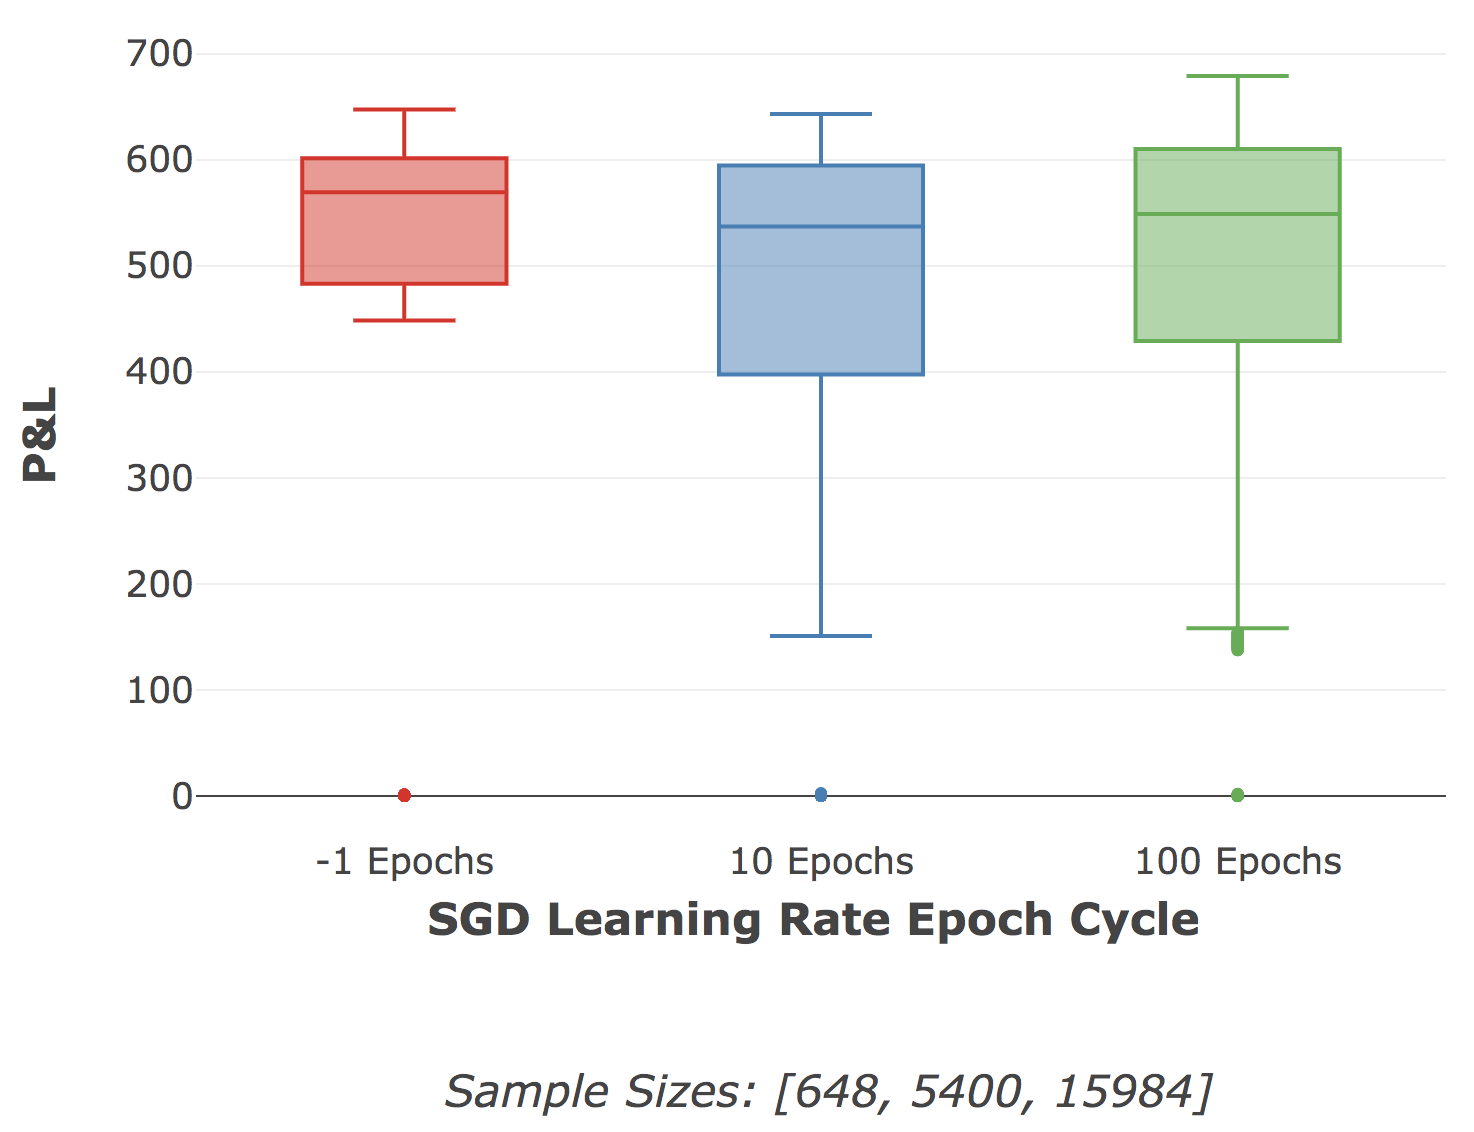
\includegraphics[scale=0.25]{images/results/network/lr/actual_pl_lr_epochs.png}
		\caption{\textbf{P\&L for Predictive Networks} 
			\newline }
		\label{figure-actual_pl_lr_epochs}
	\end{subfigure}
	\caption{Dataset: Actual10 dataset (\ref{dataset_actual10}), Configurations
		\newline Figure(a) shows the MSE scores for SAE networks, with the shorter epoch cycle offering the best (and the worst) results. Synthetic data for the SAE MSE scores behaved similarly, as seen in the appendix (section \ref{results_network_appendix}). 
		\newline In Figure (b), for the predictive networks, P\&L was highest in the 100 epoch cycle as well, where -1 indicates a constant learning rate rather than the cyclical pattern, and 10 epoch learning rates were used for configurations which only ran for 10 epochs. The configurations without learning epochs (-1) were in the second round of testing and had a more effective set of parameters elsewhere, hence the large difference in the lower bounds relative to the other configurations. Ultimately, the implementation of the learning rate cycle has offered a small but real improvement relative to the constant learning rate for P\&L.}
	\label{figure-epochs_lr}
\end{figure}


\begin{figure}[H]
	\textbf{P\&L by OGD Learning Rates}
	\centering
	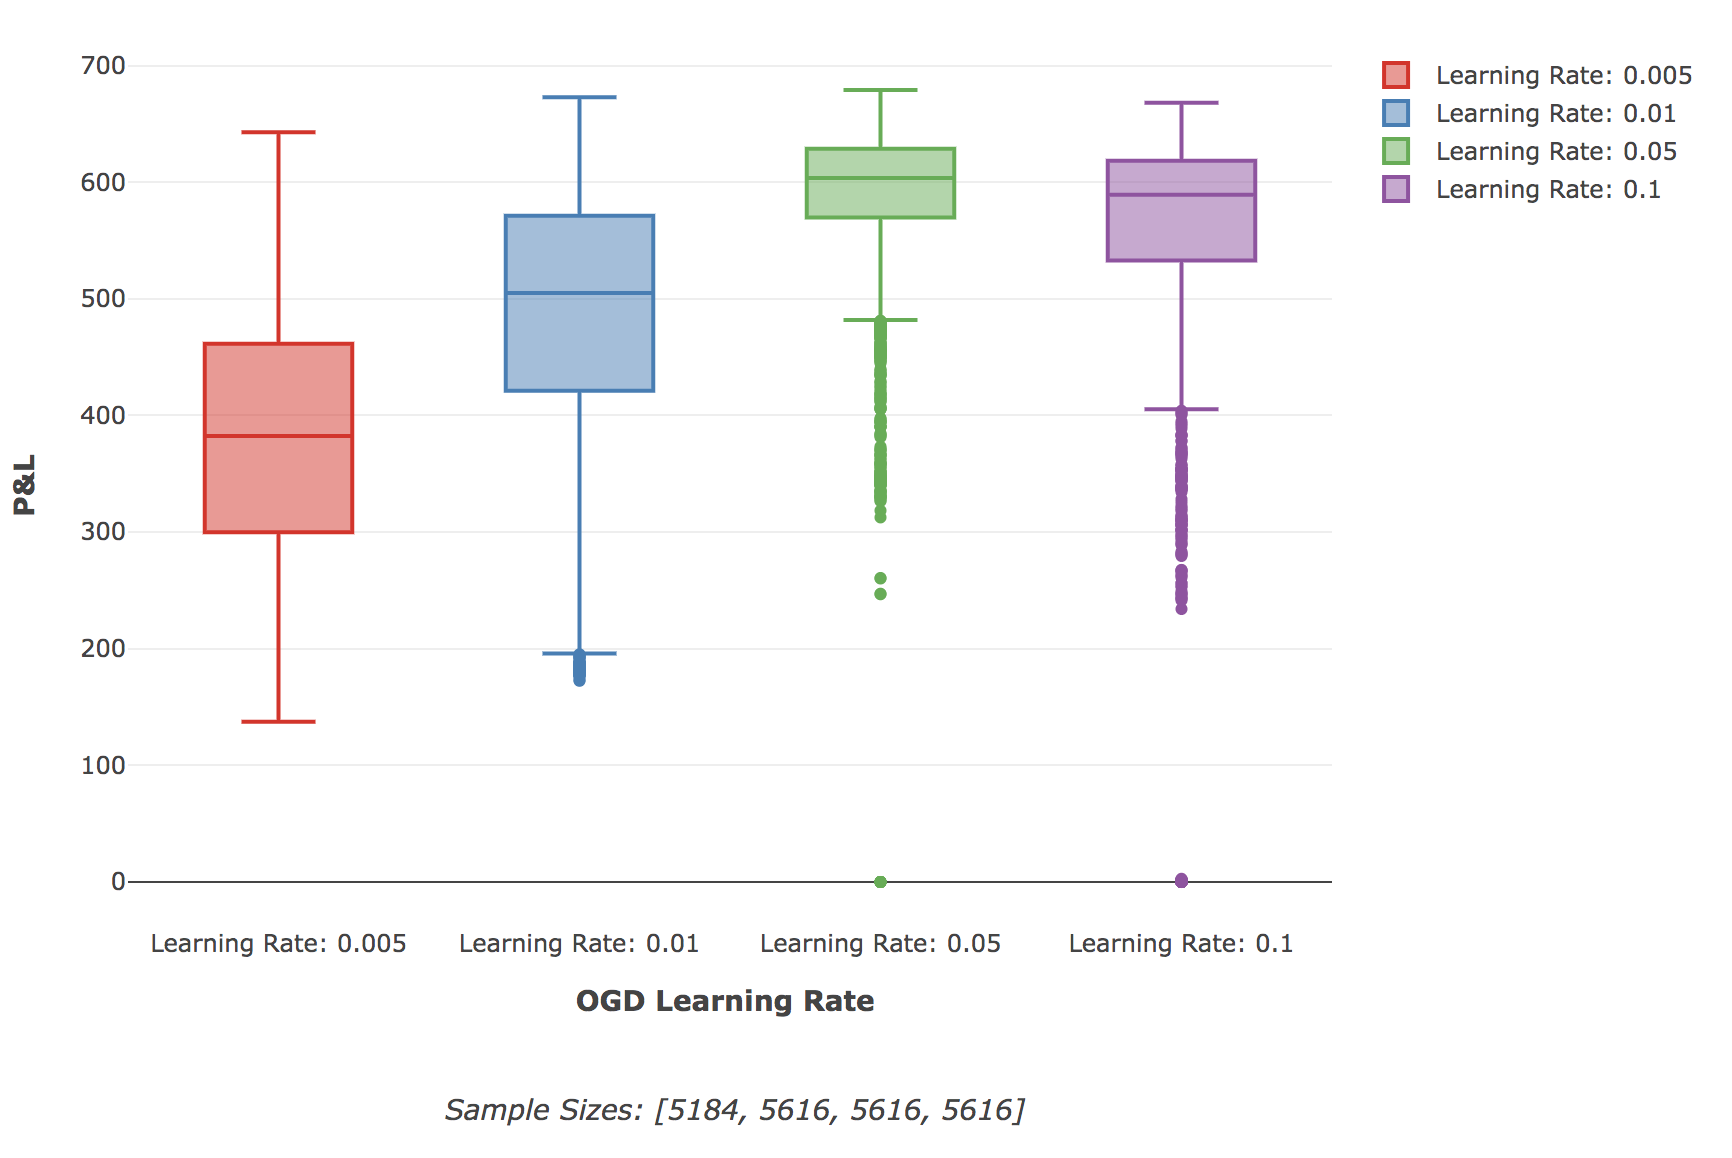
\includegraphics[scale=0.35]{images/results/network/lr/actual_ogd_lr.png}
	\caption{Dataset: Actual10 dataset (\ref{dataset_actual10}), Configurations
		\newline The P\&L performance for OGD learning rates is expectedly non-linear, with performance steadily increasing up until 0.05 where the network is adapting at the correct rate, and degrading thereafter as the network will overcorrect to noise and short term trends picked up in the online learning period. Networks trained on synthetic data showed similar trends (though were not trained past a turning point), and can be seen in the Appendix in Section \ref{results_network_appendix}.}
	\label{figure-actual_ogd_lr}
\end{figure}






\subsubsection{Effects of Regularization}


\begin{figure}[H]
	\centering
	\textbf{Effects of L1 Regularization (Actual Data)}
	\begin{subfigure}{.5\textwidth}
		\centering 
		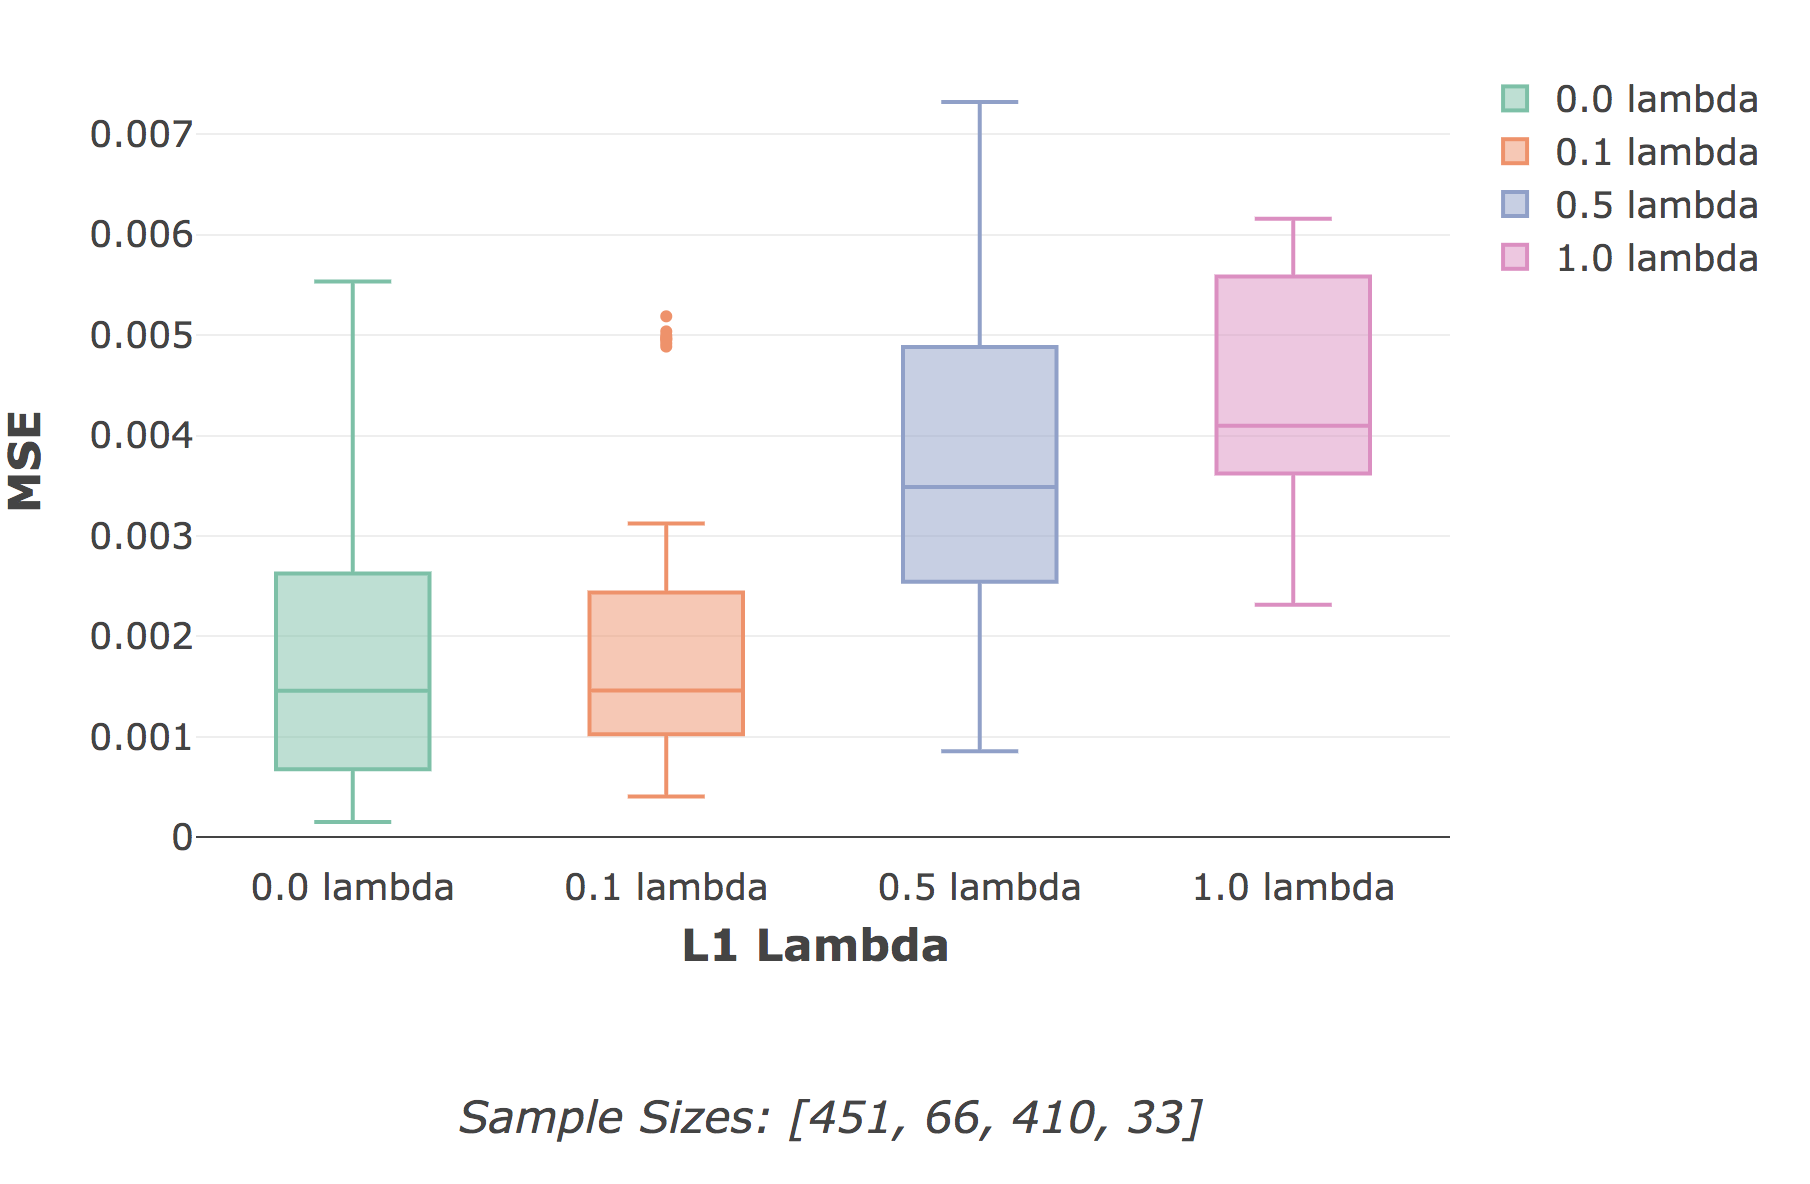
\includegraphics[scale=0.24]{images/results/network/reg/actual_mse_reg.png}
		\caption{\textbf{MSE for SAE Networks} 
			\newline }
		\label{figure-actual_mse_reg}
	\end{subfigure}%
	\begin{subfigure}{.5\textwidth}
		\centering 
		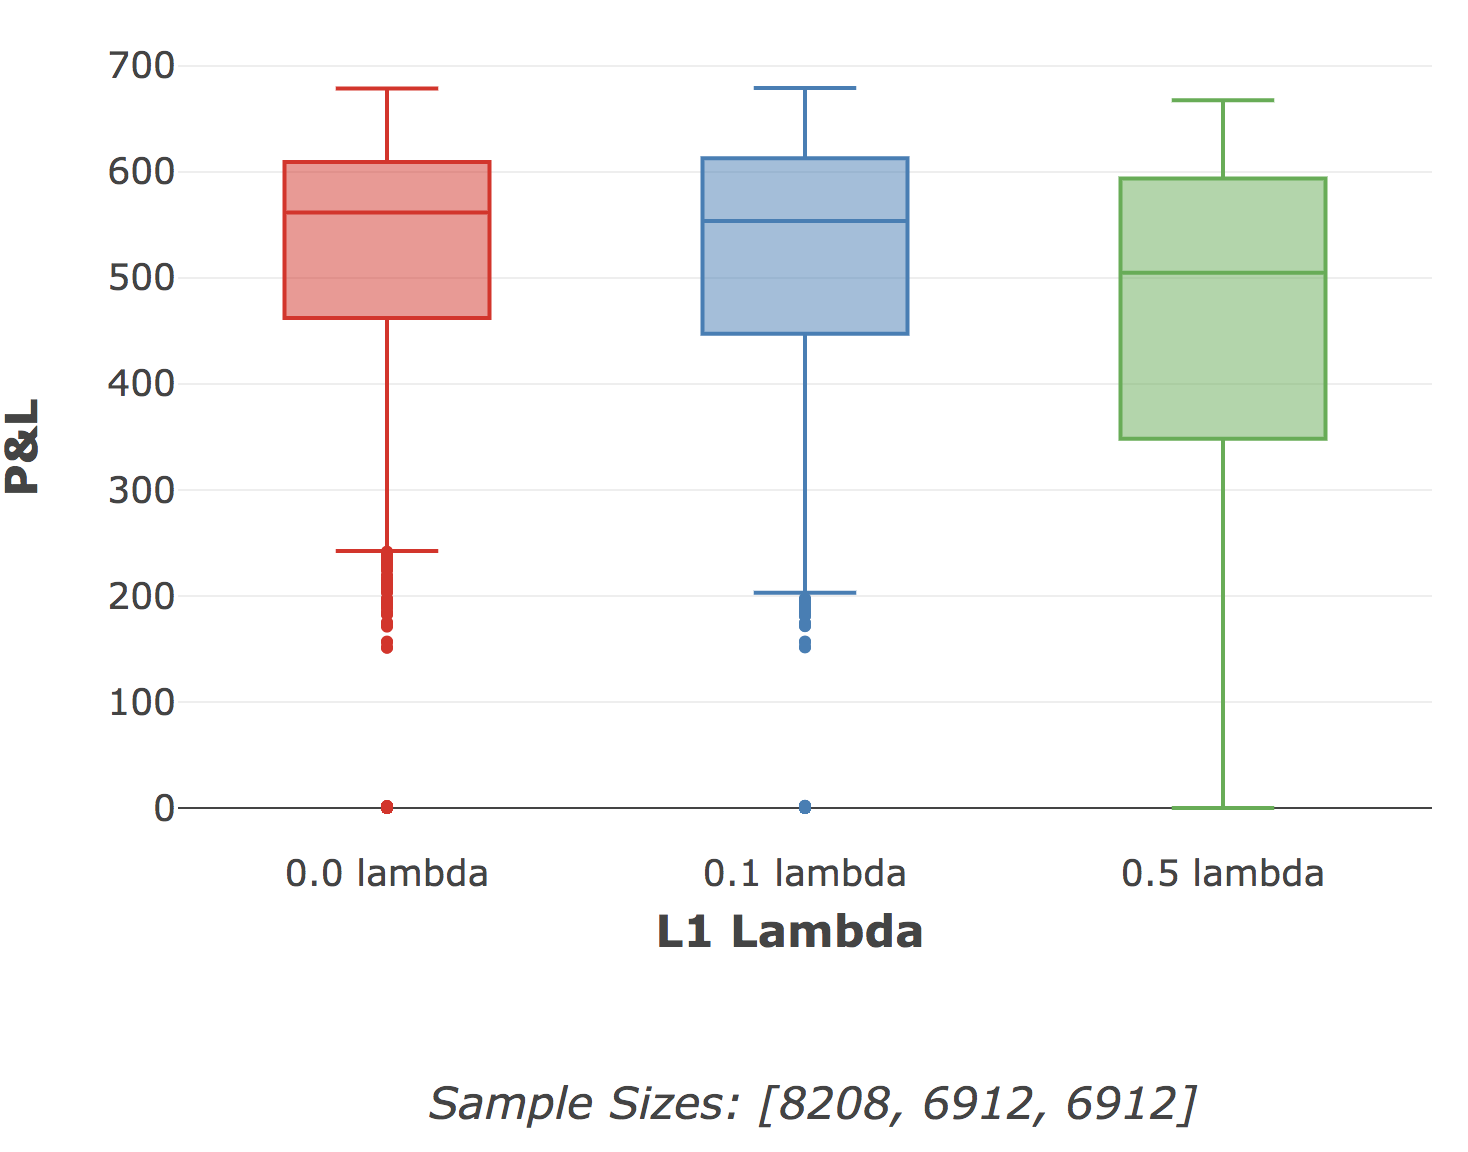
\includegraphics[scale=0.24]{images/results/network/reg/actual_pl_reg.png}
		\caption{\textbf{P\&L for Predictive Networks} 
			\newline }
		\label{figure-actual_pl_reg}
	\end{subfigure}
	\caption{Dataset: Actual10 dataset (\ref{dataset_actual10}), Configurations
		\newline }
	\label{figure-results-reg}
\end{figure}

\subsubsection{Effects of Denoising}

\begin{figure}[H]
	\centering
	\textbf{Effects of Denoising on SAE MSE (Actual Data)}
	\begin{subfigure}{.5\textwidth}
		\centering 
		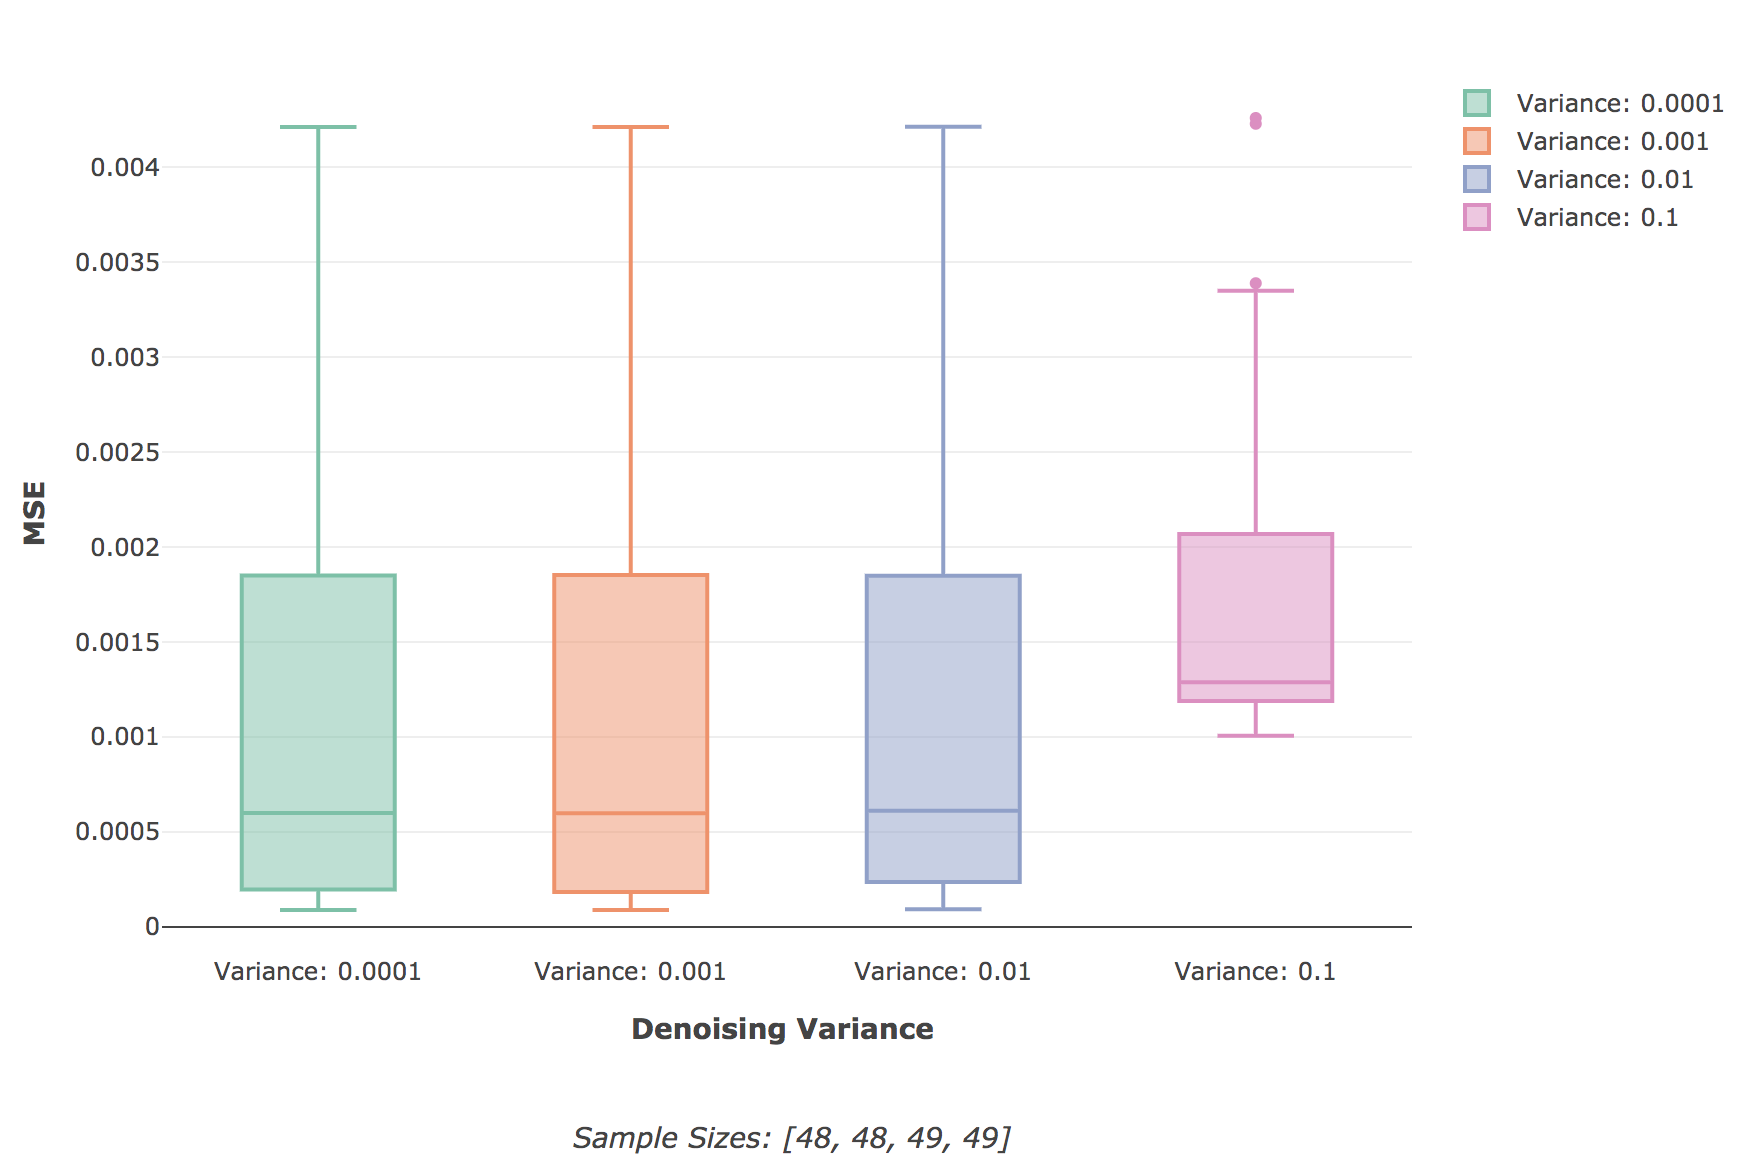
\includegraphics[scale=0.24]{images/results/network/denoising/actual_mse_gaussian.png}
		\caption{\textbf{Gaussian Denoising} 
			\newline }
		\label{figure-actual_mse_gaussian}
	\end{subfigure}%
	\begin{subfigure}{.5\textwidth}
		\centering 
		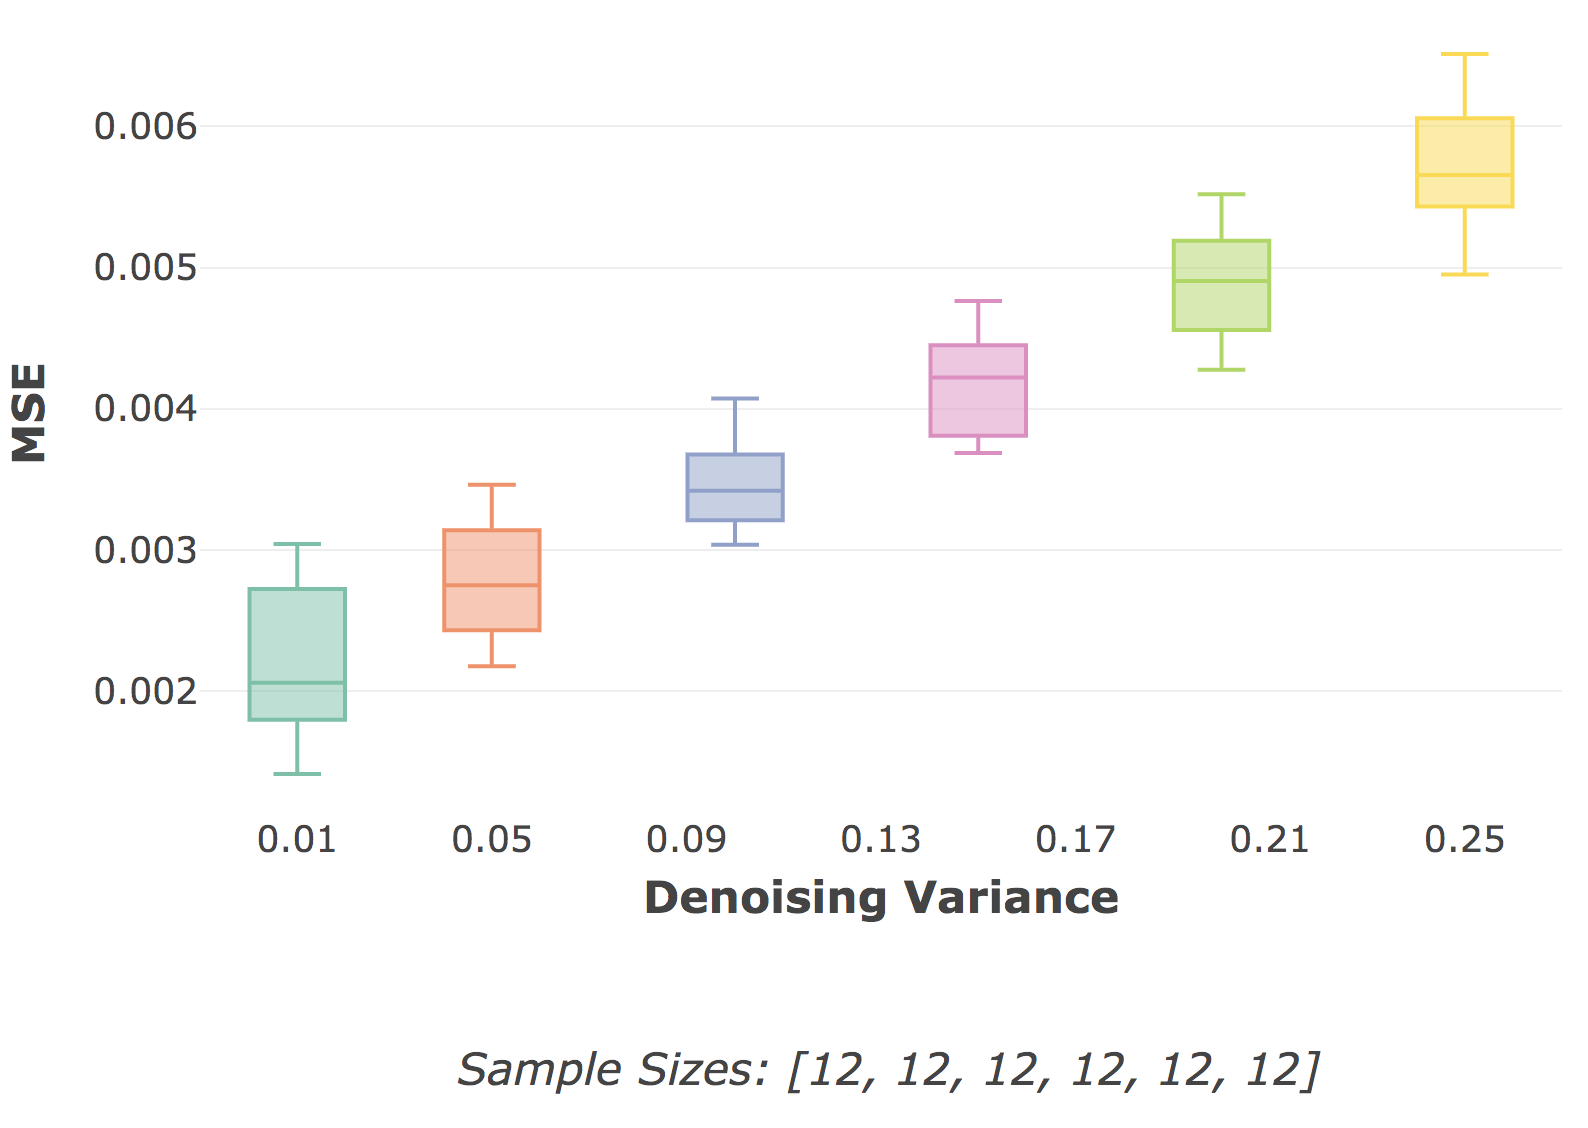
\includegraphics[scale=0.24]{images/results/network/denoising/actual_mse_masking.png}
		\caption{\textbf{Masking Denoising} 
			\newline }
		\label{figure-actual_mse_masking}
	\end{subfigure}
	\caption{Dataset: , Configurations
		\newline }
	\label{figure-results_mse_denoising}
\end{figure}

\begin{figure}[H]
	\textbf{P\&L by Masking Denoising}
	\centering
	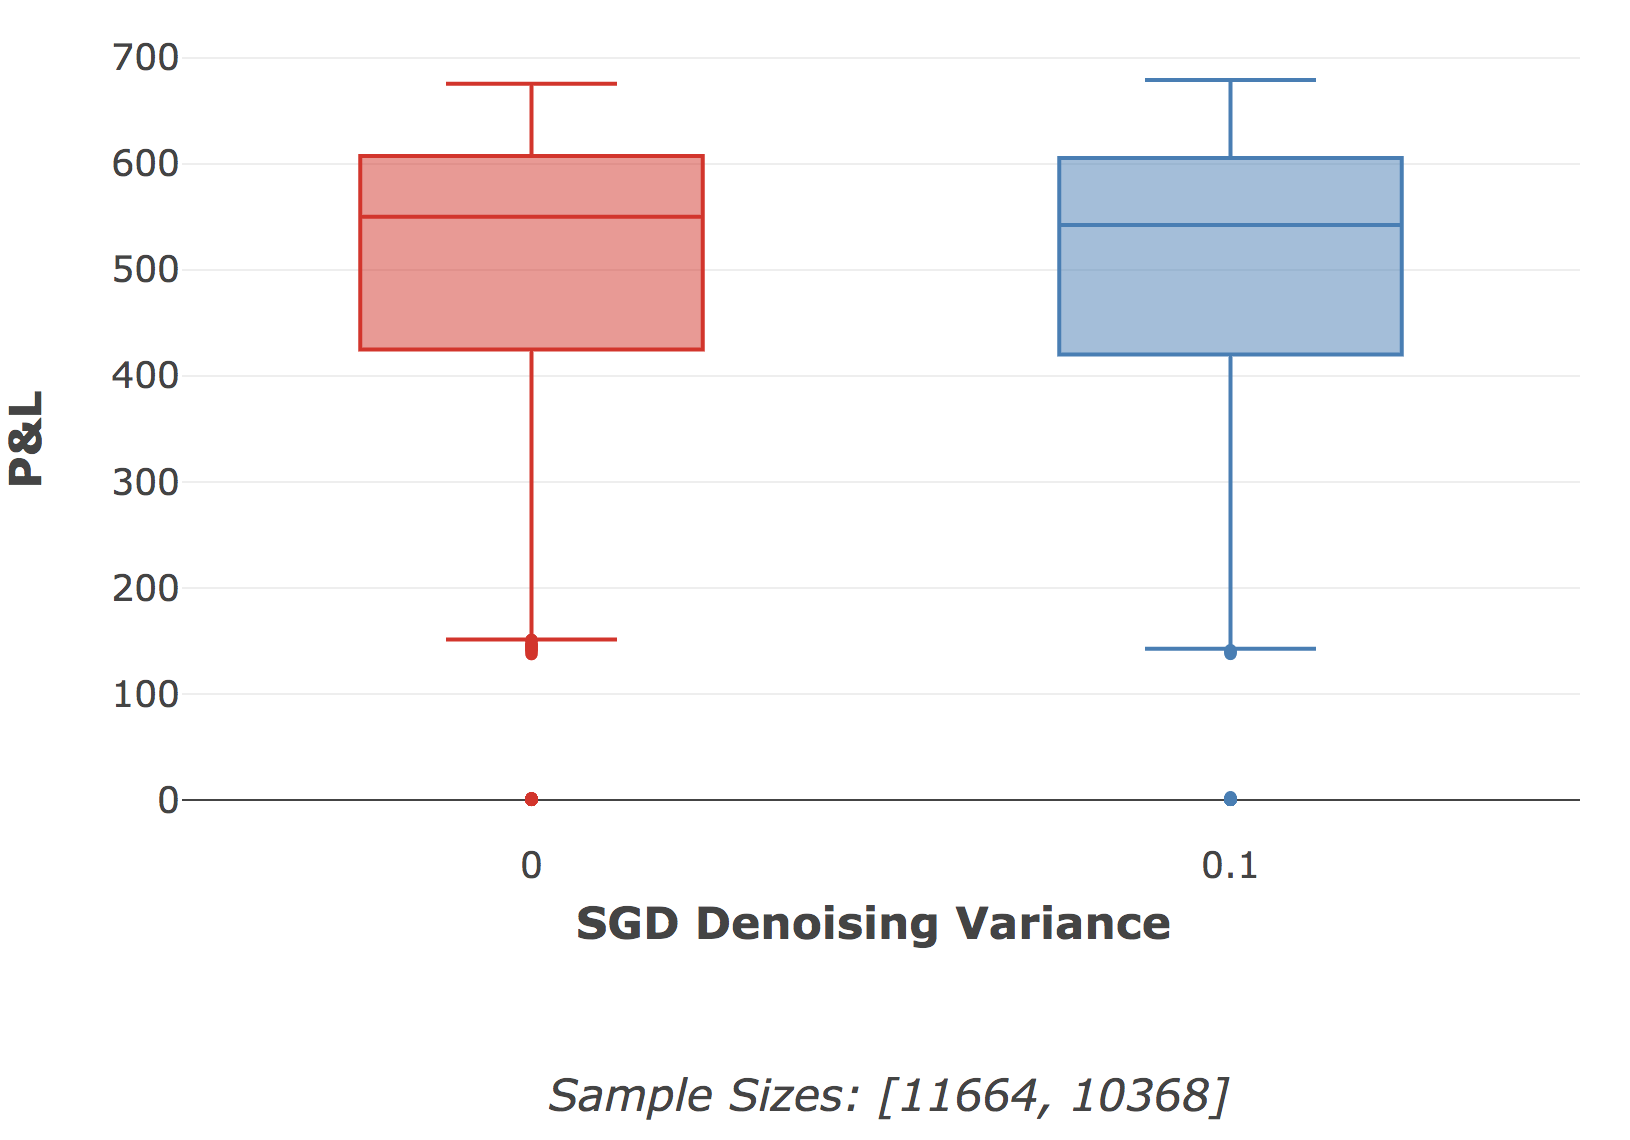
\includegraphics[scale=0.35]{images/results/network/denoising/actual_pl_masking.png}
	\caption{Dataset: Actual10 dataset (\ref{dataset_actual10}), Configurations
		\newline }
	\label{figure-actual_pl_masking}
\end{figure}



\newpage
\subsection{The Effects of Data Aggregation and Value of Historical Data}\label{results_hist}

Input data was scaled to 3 different configurations across a series of tests in order to assess the effect of shorter and longer configurations on both SAE MSE performance, as well as the predictive predictive P\&L results. The configurations tested (in trading day window periods) were:

\begin{itemize}
	\item[1.] [1, 5, 20]
	\item[2.] [5, 20, 60]
	\item[3.] [10, 20, 60]
\end{itemize}

By way of example using the 3rd configuration: the implementation of this is such that at each time point considered by a network the log difference changes for the past 10, 20 and 60 days are available for each asset. This is described more extensively in Chapter \ref{Data}.\newline

Sections \ref{results_data_mse} and \ref{results_data_pl} discuss the effects of data aggregation windows on SAE MSE and predictive P\&L performance, showing that shorter windows are easier to replicate in SAE networks, and that P\&L is improved through access to the most recent fluctuations (i.e. 1 day) and then longer medium term trends. Section \ref{results_data_hist} then discusses and validates the idea that extensive historical data is of limited use when having to make predictions for 1 week price changes in more recent data.

\subsubsection{Data Aggregation and SAE MSE Scores}\label{results_data_mse}

\begin{figure}[H]
	\centering
	\textbf{SAE MSE Scores for Synthetic Data}
	\begin{subfigure}{.5\textwidth}
		\centering 
		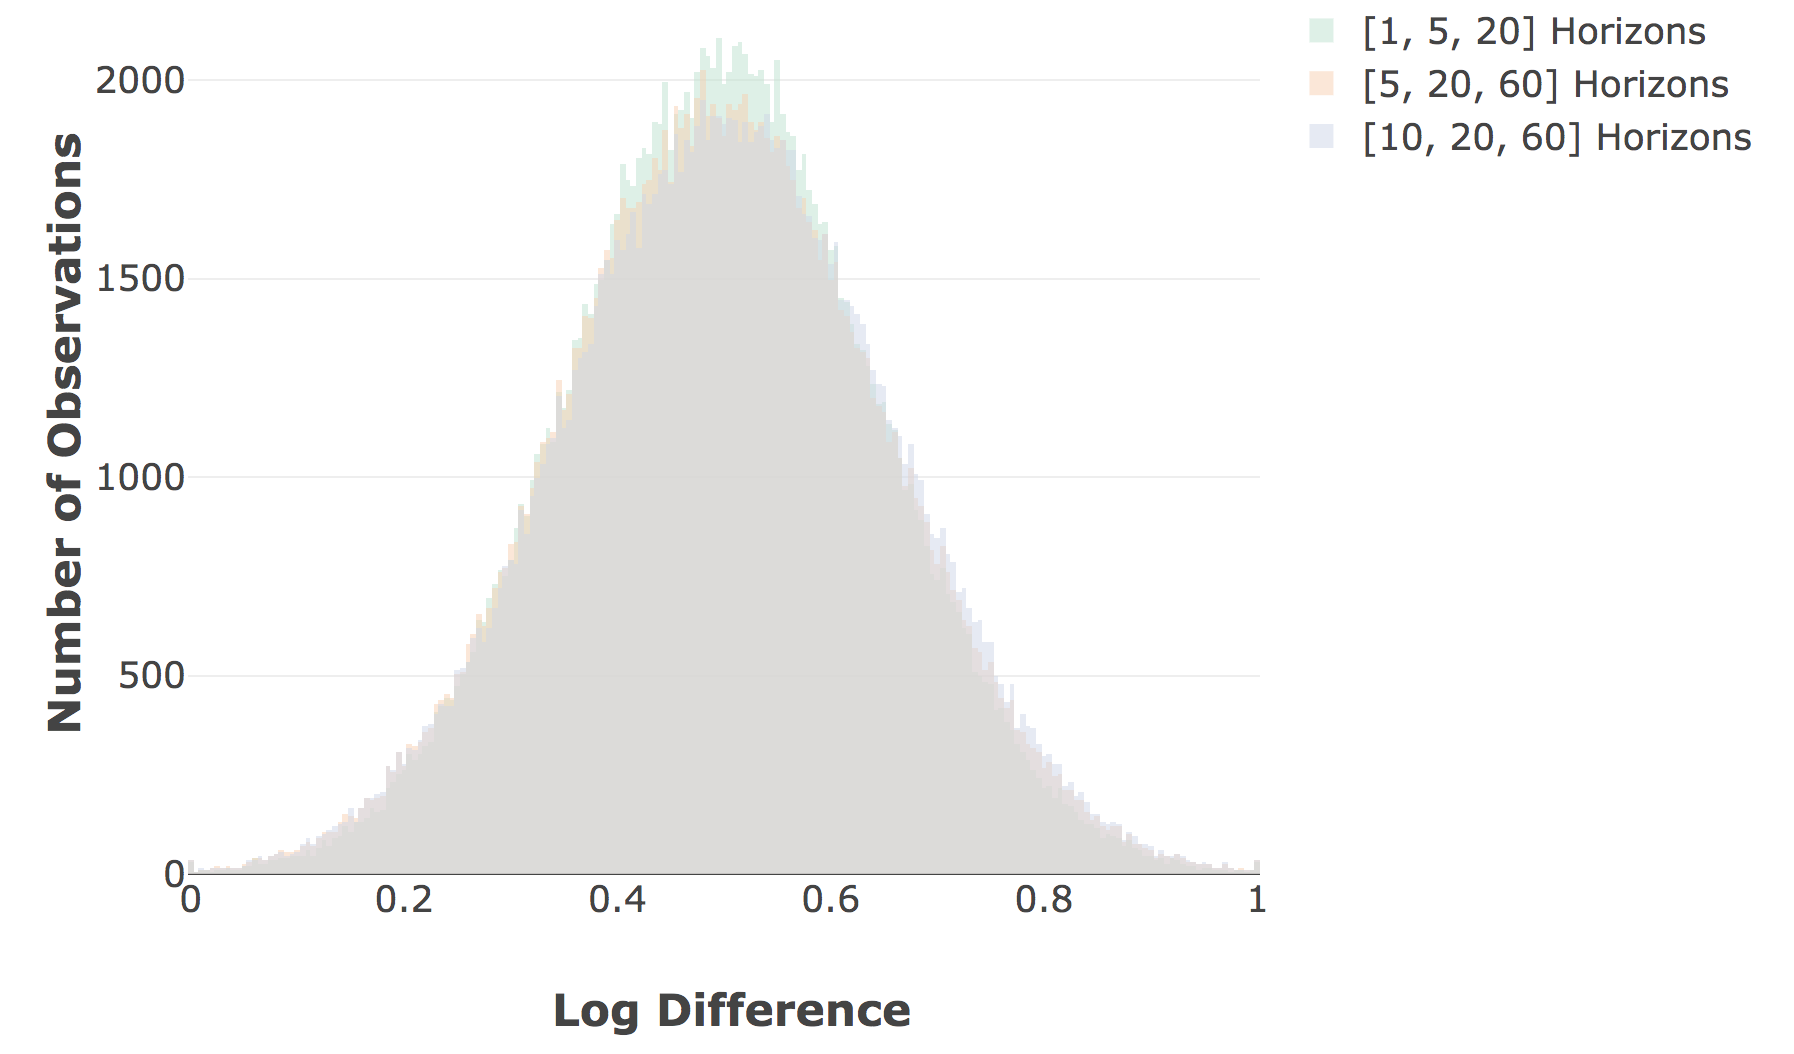
\includegraphics[scale=0.25]{images/results/data/test_aggregate_dist.png}
		\caption{\textbf{Log Difference Distributions} 
			\newline }
		\label{figure-test_aggregate_dist}
	\end{subfigure}%
	\begin{subfigure}{.5\textwidth}
		\centering 
		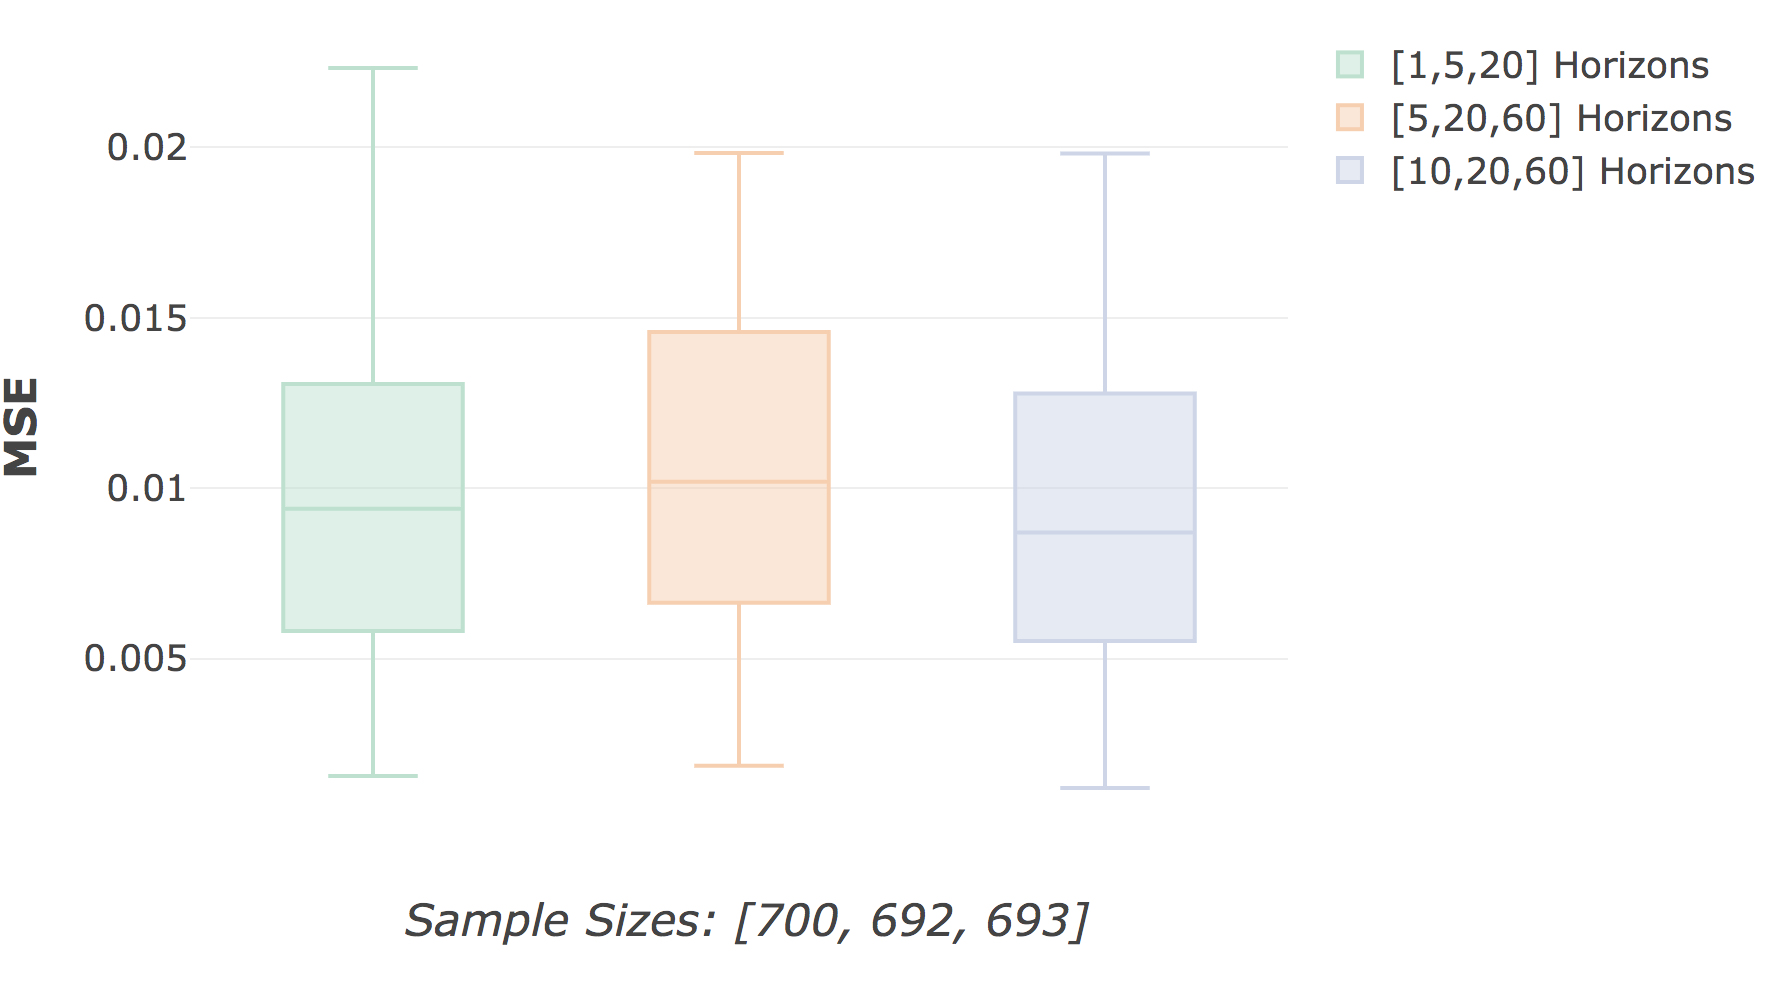
\includegraphics[scale=0.26]{images/results/data/test_aggregation_mse.png}
		\caption{\textbf{SAE MSE Scores} 
			\newline }
		\label{figure-test_aggregation_mse}
	\end{subfigure}
	\caption{Dataset: Synthetic10 dataset (\ref{dataset_synthetic10}), Configuration 
		\newline Figure (a) shows the distribution of values to be replicated by the SAE for synthetic data. Geometric Brownian Motion generates discrete changes that follow a log-normal distribution, the log difference and scaling of which (as per the data processing described in \ref{data_processing}) result in normally distributed price changes. We see small differences in the distributions according to the data aggregation used, as one would expect, with slightly lower variances occuring for smaller data windows ($\sigma_{[1,5,20]} = 0.145$, $\sigma_{[5,20,60]} = 0.152$, $\sigma_{[10,20,60]} = 0.154$). There were some differences in SAE performance as indicated in Figure (b), though not to large extents and considering the very similar distribution of values, there isn't any expectation of seeing fundamental differences in the networks ability to compress and replicate them. }
	\label{figure-data_sae_synthetic}
\end{figure}

\begin{figure}[H]
	\centering
	\textbf{SAE MSE Scores for Actual Data}
	\begin{subfigure}{.5\textwidth}
		\centering 
		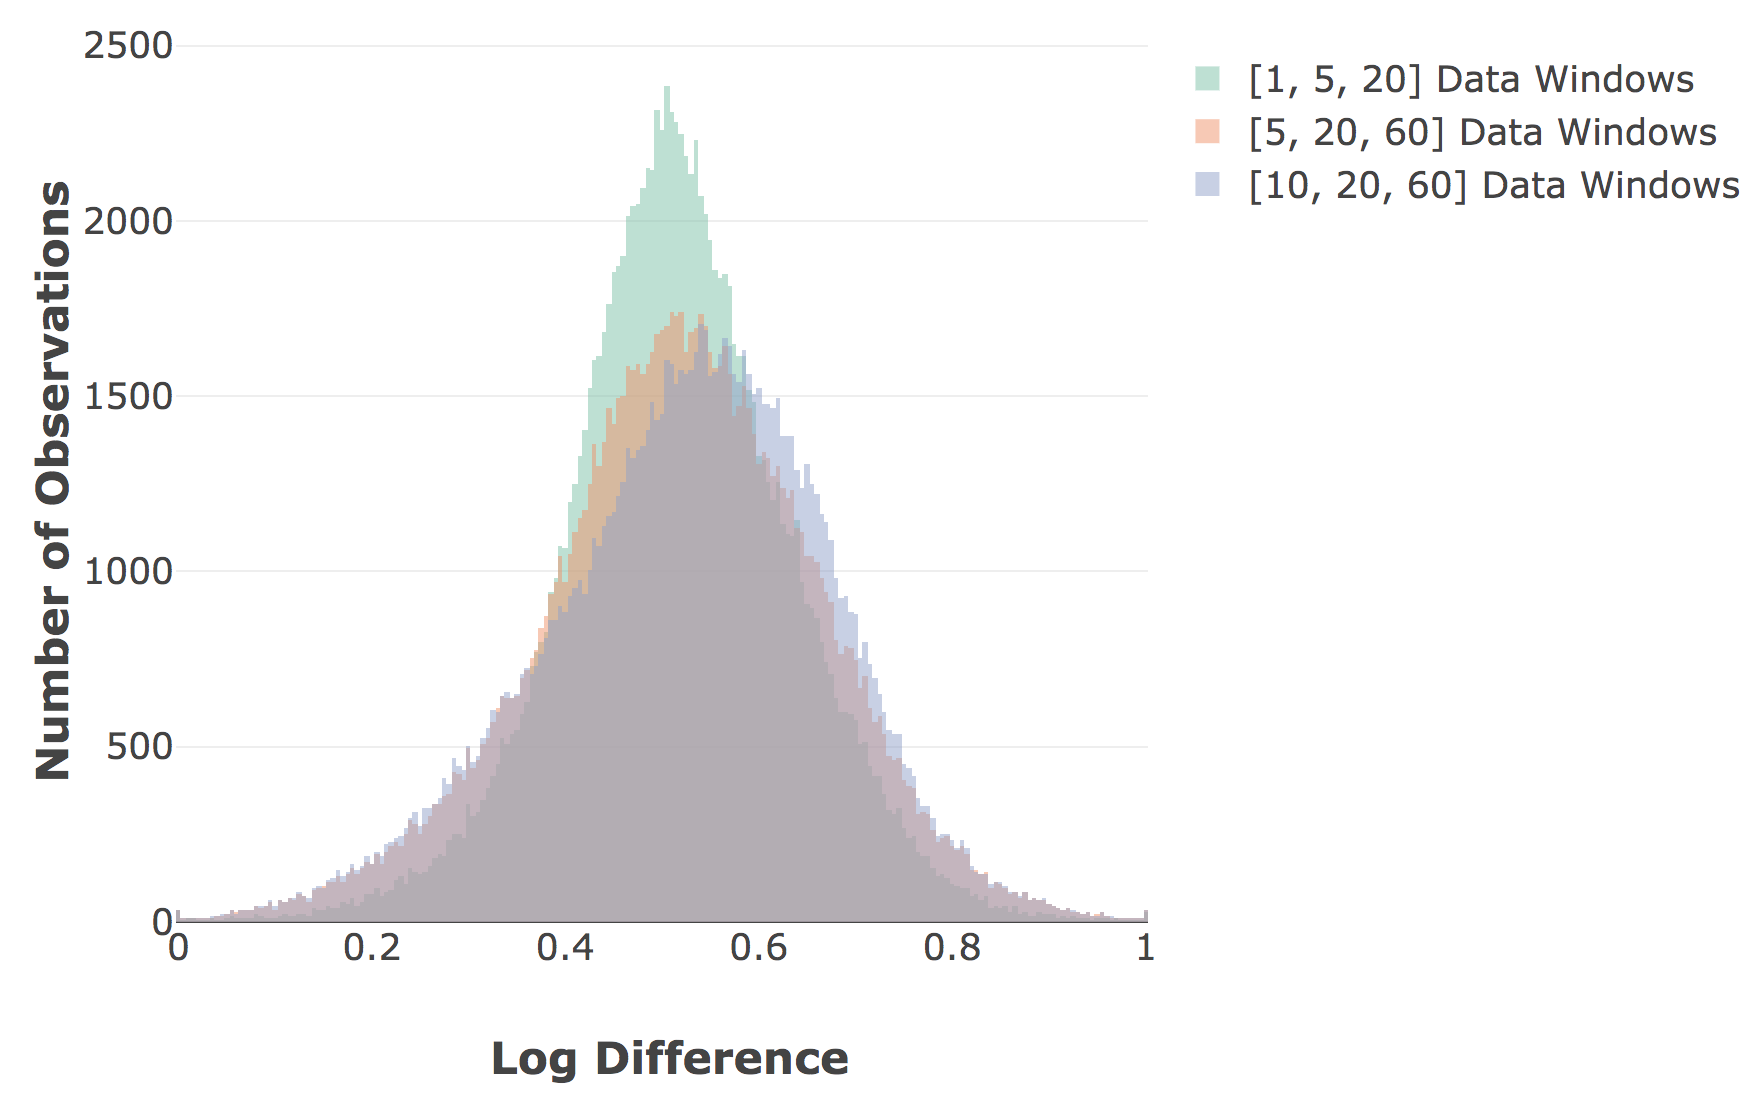
\includegraphics[scale=0.25]{images/results/data/actual_aggregate_dist.png}
		\caption{\textbf{Log Difference Distribution}
			\newline }
		\label{figure-actual_aggregate_dist}
	\end{subfigure}%
	\begin{subfigure}{.5\textwidth}
		\centering 
		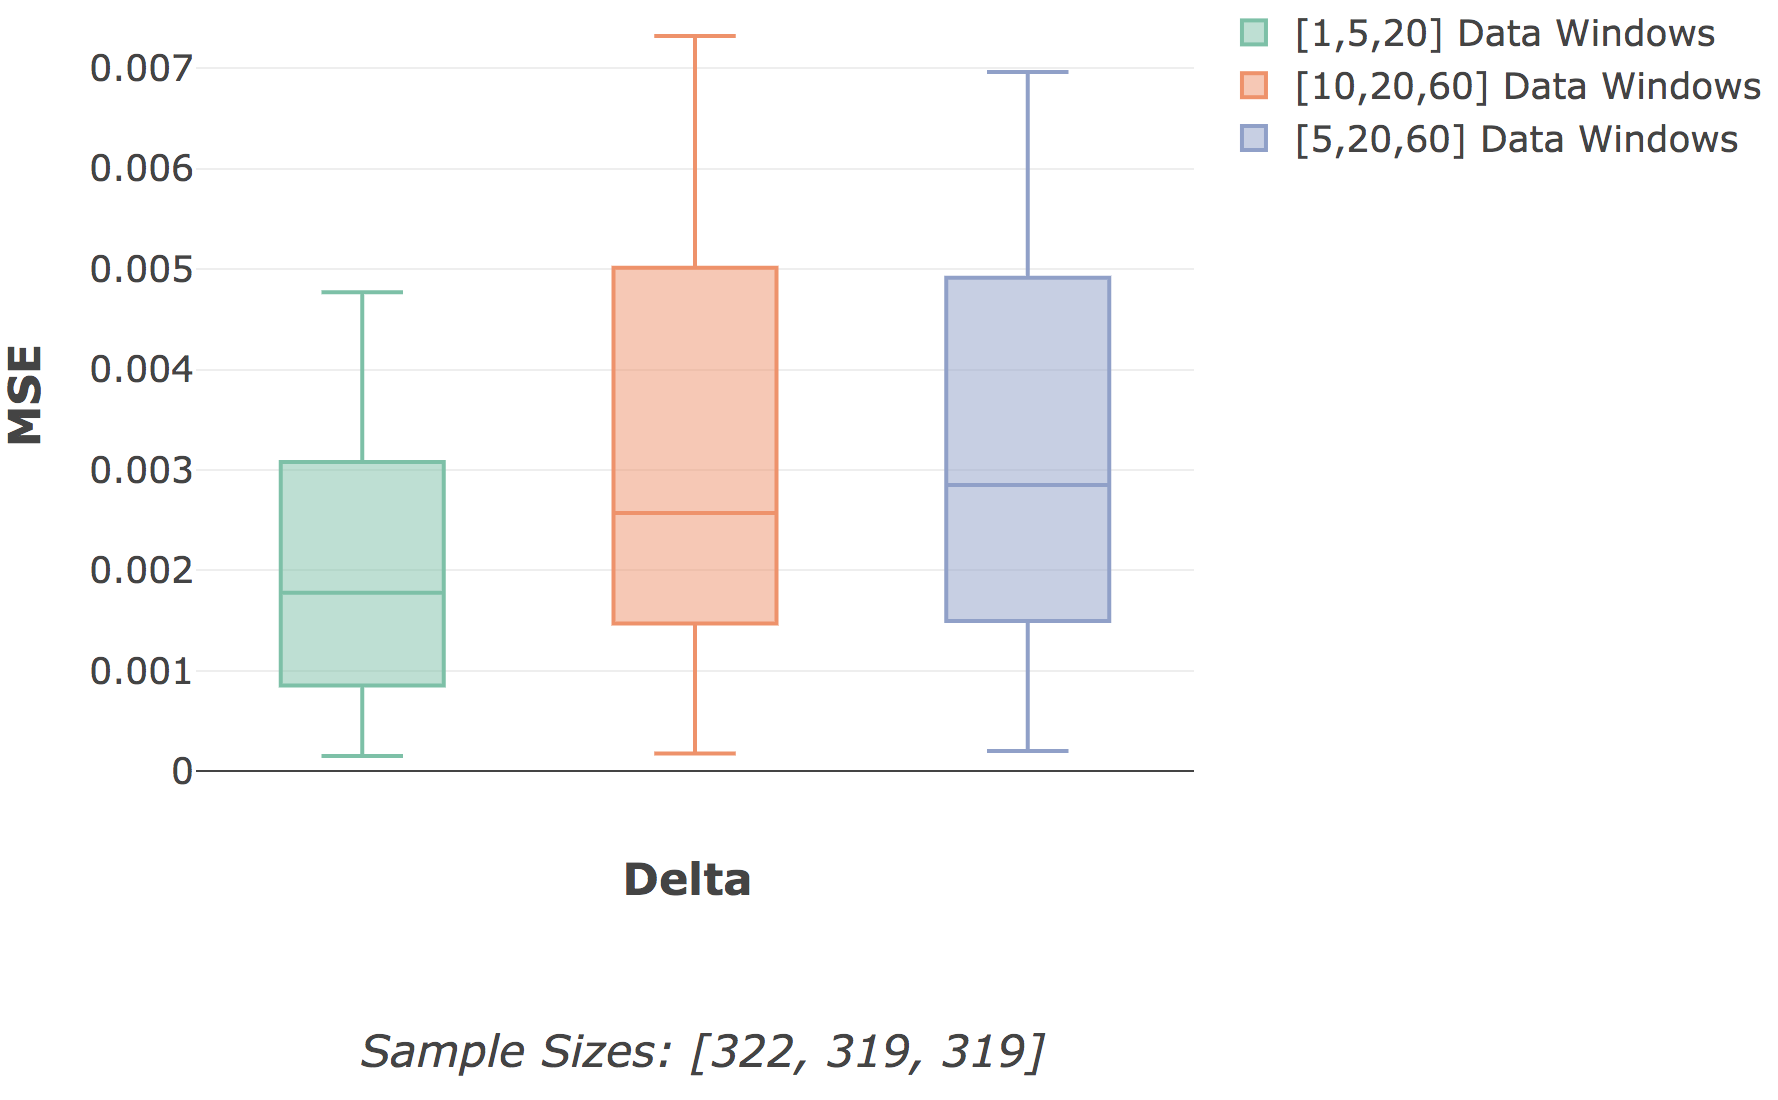
\includegraphics[scale=0.26]{images/results/data/actual_aggregation_mse.png}
		\caption{\textbf{SAE MSE Scores} 
			\newline }
		\label{figure-actual_aggregation_mse}
	\end{subfigure}
	\caption{Dataset: Actual10 dataset (\ref{dataset_actual10}), Configuration 
		\newline Figure (a) shows the distribution of values to be replicated by the SAE for actual data. The distributions are noticeably different from synthetic data, as there is no prior on the price change values, and so variances differ far more across the configurations ($\sigma_{[1,5,20]} = 0.118$, $\sigma_{[5,20,60]} = 0.146$, $\sigma_{[10,20,60]} = 0.150$). Smaller data windows are less likely to capture larger fundamental price changes, resulting in the lower variances. This in turn, makes for easier replication for the SAE networks due to less variety in the sample set, which is seen in Figure (b) with the noticeably better performance in the [1, 5, 20] configuration.   }
	\label{fig:data_sae_actual}
\end{figure}


\subsubsection{Data Aggregation and Predictive P\&L Scores}\label{results_data_pl}

\begin{figure}[H]
	\centering 
	\textbf{P\&L by Data Aggregation (Synthetic Data)}
	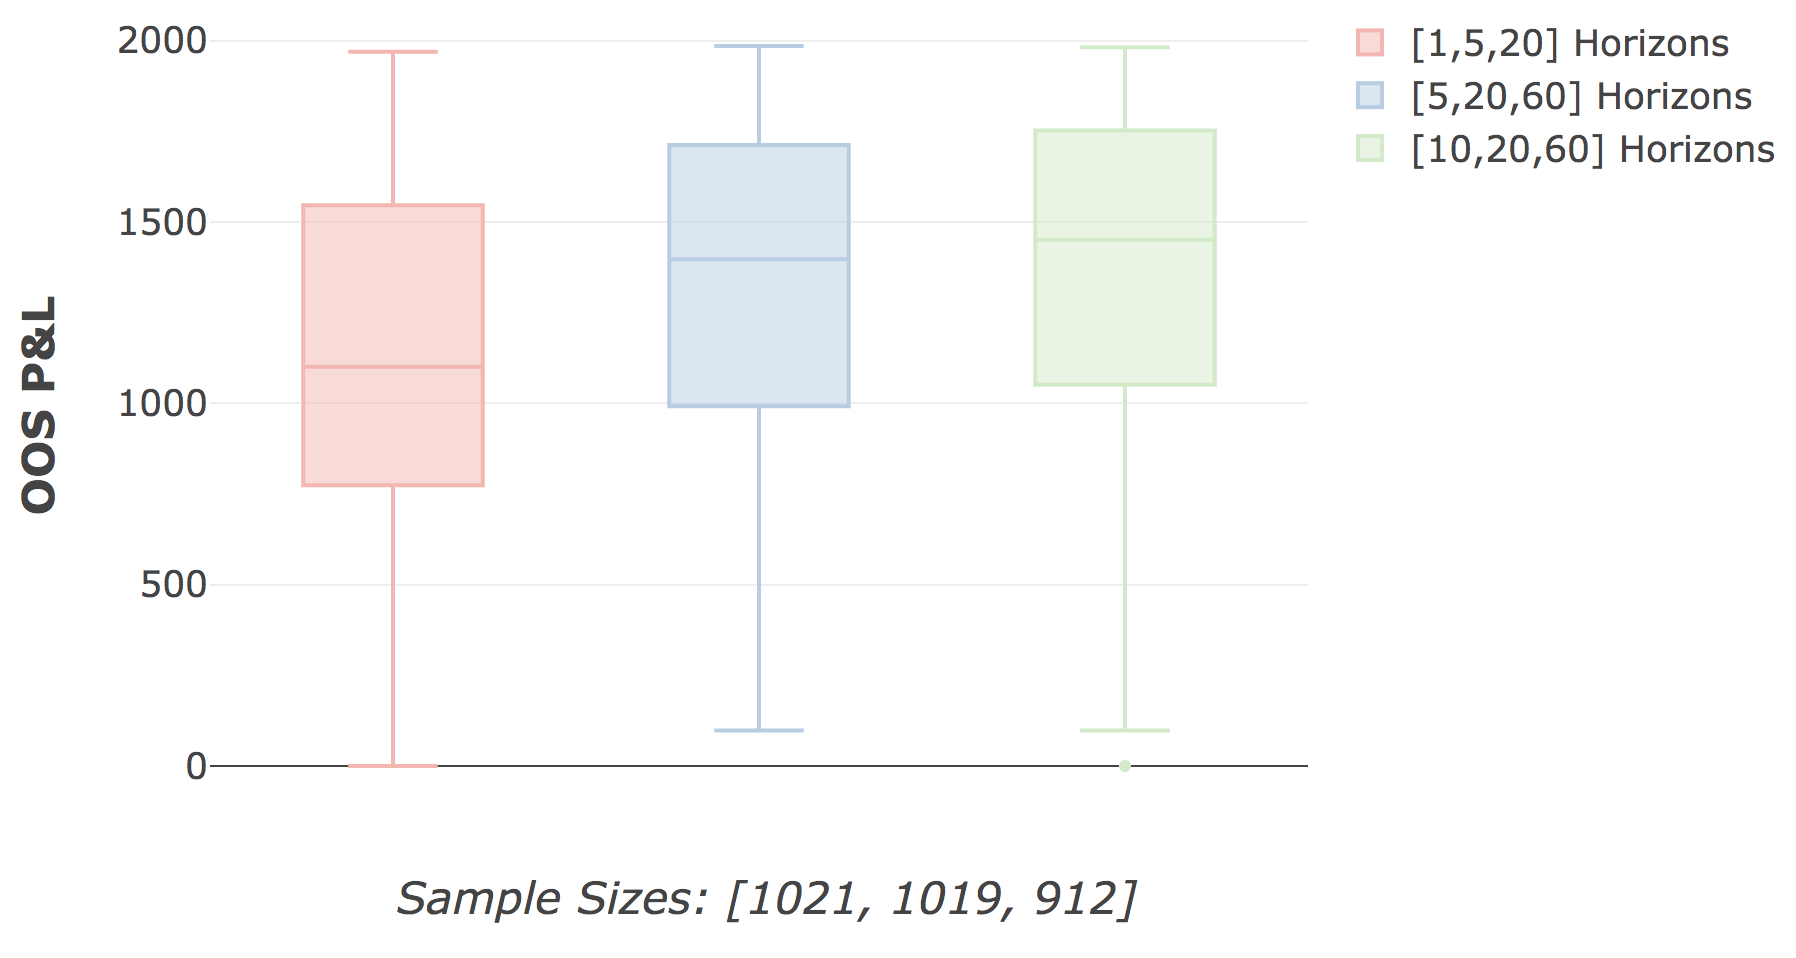
\includegraphics[scale=0.4]{images/results/data/test_aggregation_pl.png}
	\caption{
		Dataset: Synthetic10 dataset (\ref{dataset_synthetic10}), Configuration 
		\newline  The boxplots here show the P\&L from the MMS according group by the data window configurations. There's a clear trend of P\&L increasing as the length of the windows increase. Shorter term GBM data would be more likely to represent fluctuations, whereas the longer term windows will be more representative of the constant mean in the stocks, leading to easier predictive performance and higher P\&L.}
	\label{figure-test_aggregation_pl}
\end{figure}

\begin{figure}[H]
	\centering 
	\textbf{P\&L by Data Aggregation (Actual Data) }
	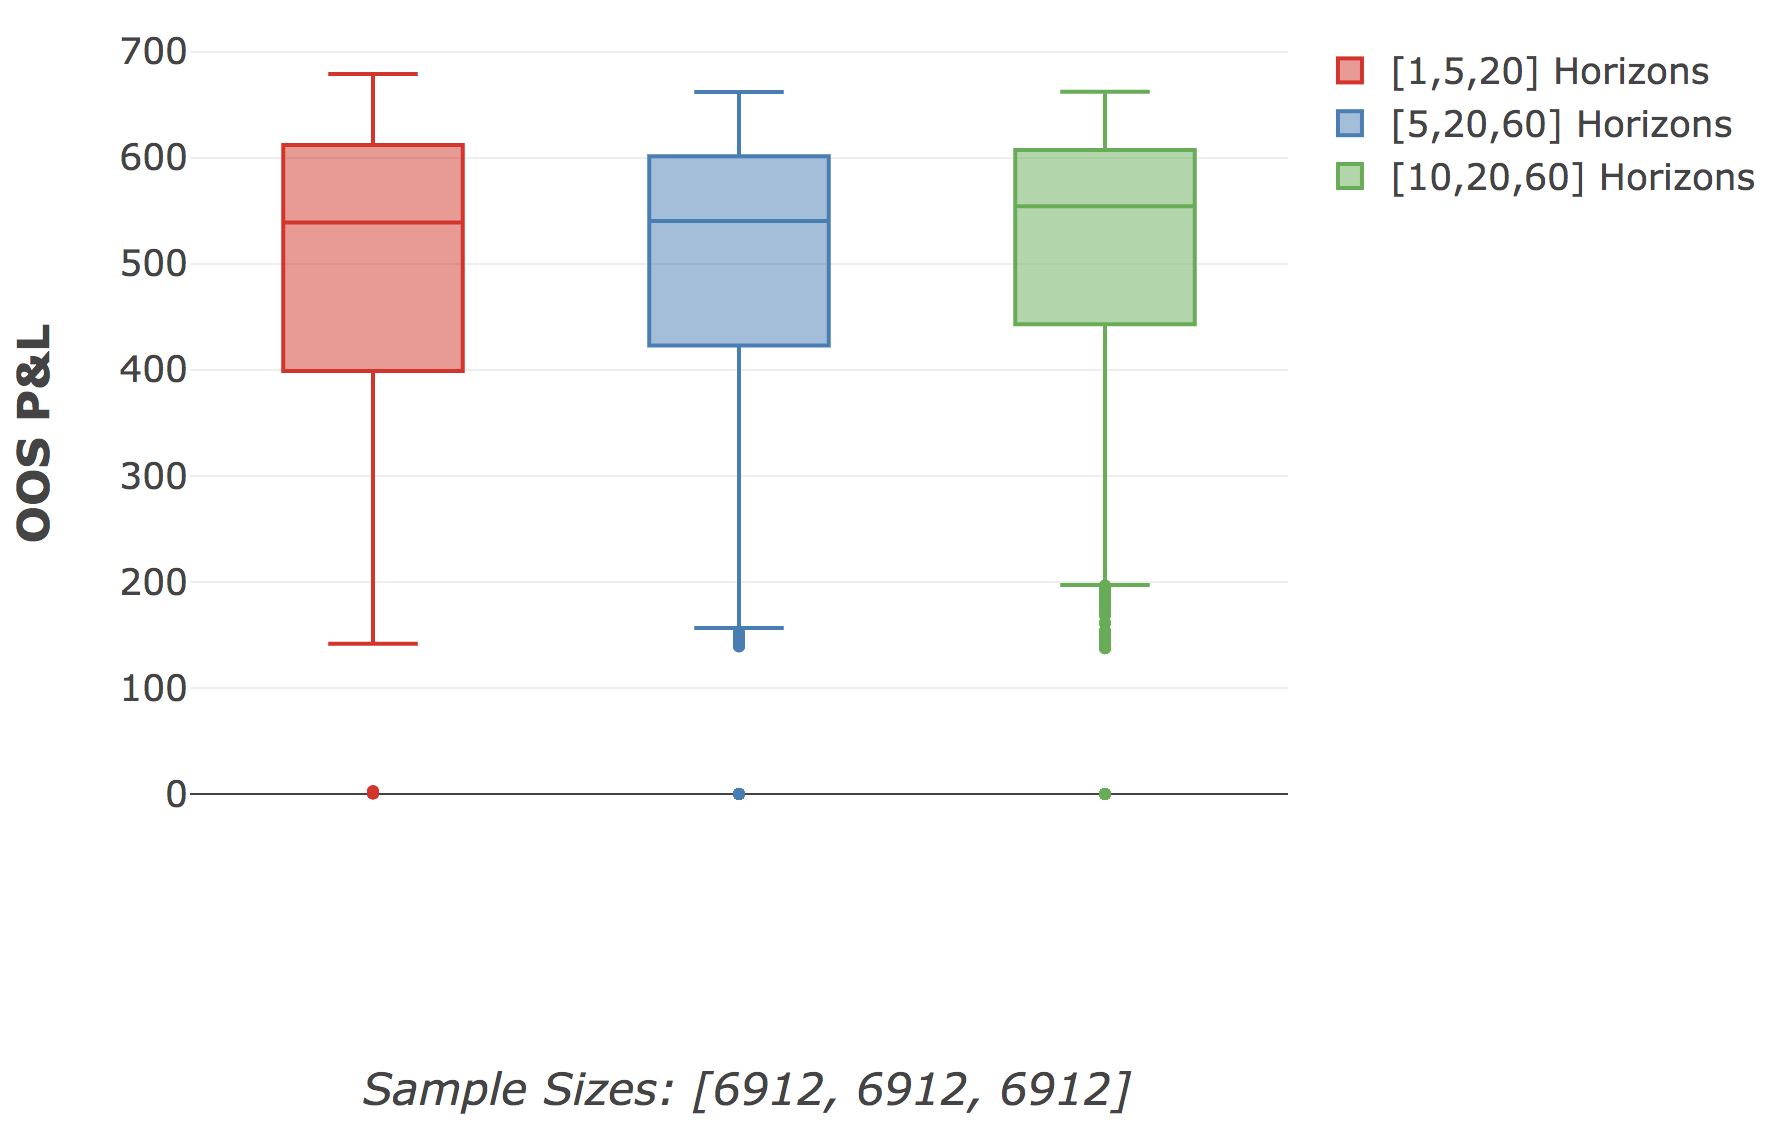
\includegraphics[scale=0.4]{images/results/data/actual_aggregation_pl.png}
	\caption{
		Dataset: Actual10 dataset (\ref{dataset_actual10}), Configuration 
		\newline The P\&L by data window configurations for actual data show a more complex view. At a general level, predictive performance is increasing as the span of the windows increase. However, the highest P\&L occurs for the shortest window configuration ([1, 5, 20]). The suggestion here is that both long term trends and short term fluctuations are useful for making short term predictions in price changes, but that a middle of the road configuration offers the worst of both dynamics.}
	\label{figure-actual_aggregation_pl}
\end{figure}

\subsubsection{Effects of IS Training and Historical Data}\label{results_data_hist}

Experimental configuration sets were run to test the hypothesis that the amount of historical IS data available is of limited use, and that the real value is in broader current and cross sectional data. This idea is in line with the understanding that financial markets are inherently complex, adaptive and dynamic, as discussed more broadly in section \ref{lr_TechnicalAnalysis}. With this in mind, and especially so in light of a fundamentally changing macroeconomic landscape, there is limited reason to believe that the functions and relations that may have governed the asset prices 10-15 years ago would still be in effect today. The P\&L results shown in Figures \ref{figure-results_pl_max_epochs} and \ref{figure-results_it3_validationset} validate this and suggeset that extensive training on past data may be akin to pre-training network weights at best, and counterproductive in overfitting to dynamics that no longer exist at worst.



\begin{figure}[H]
	\centering 
	\textbf{P\&L by IS Training Epochs}
	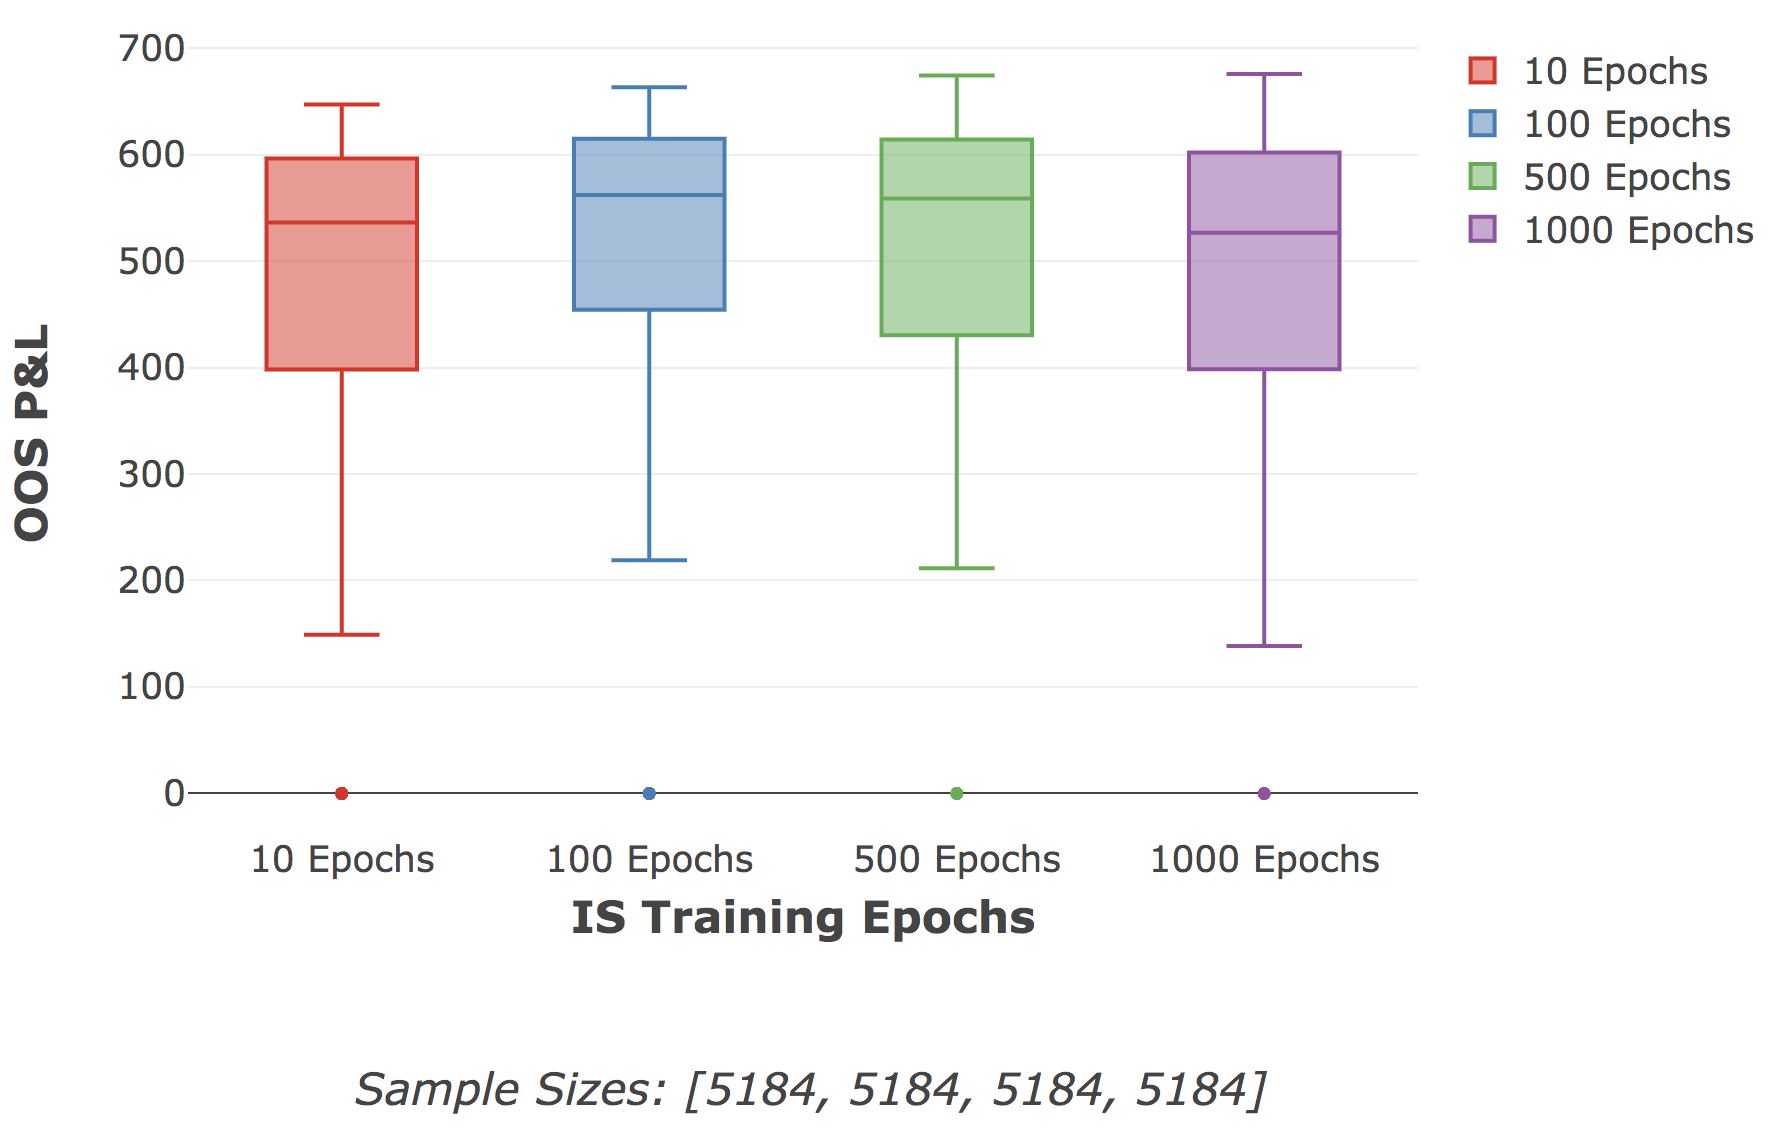
\includegraphics[scale=0.32]{images/results/data/max_epochs.png}
	\caption{
		Dataset: Actual10 dataset (\ref{dataset_actual10}), Configuration 
		\newline The box plots above show P\&L grouped by the number of epochs in the SGD IS training phase (i.e. the number of times the IS data was trained on). In this set of configurations, 100 Epochs offers the best overall performance, and further training to 500 or 1000 epochs degrades performance due to the network overfitting on the IS data. The results here are noteworthy as they suggest the benefit of historical data is limited - having a network become better at predicting returns 10 years ago is not leading to increased P\&L for more current data. The small difference between 10 and 100 Epochs further emphasises this point.
	}
	\label{figure-results_pl_max_epochs}
\end{figure}


\begin{figure}[H]
	\centering 
	\textbf{P\&L by IS Training Dataset Size}
	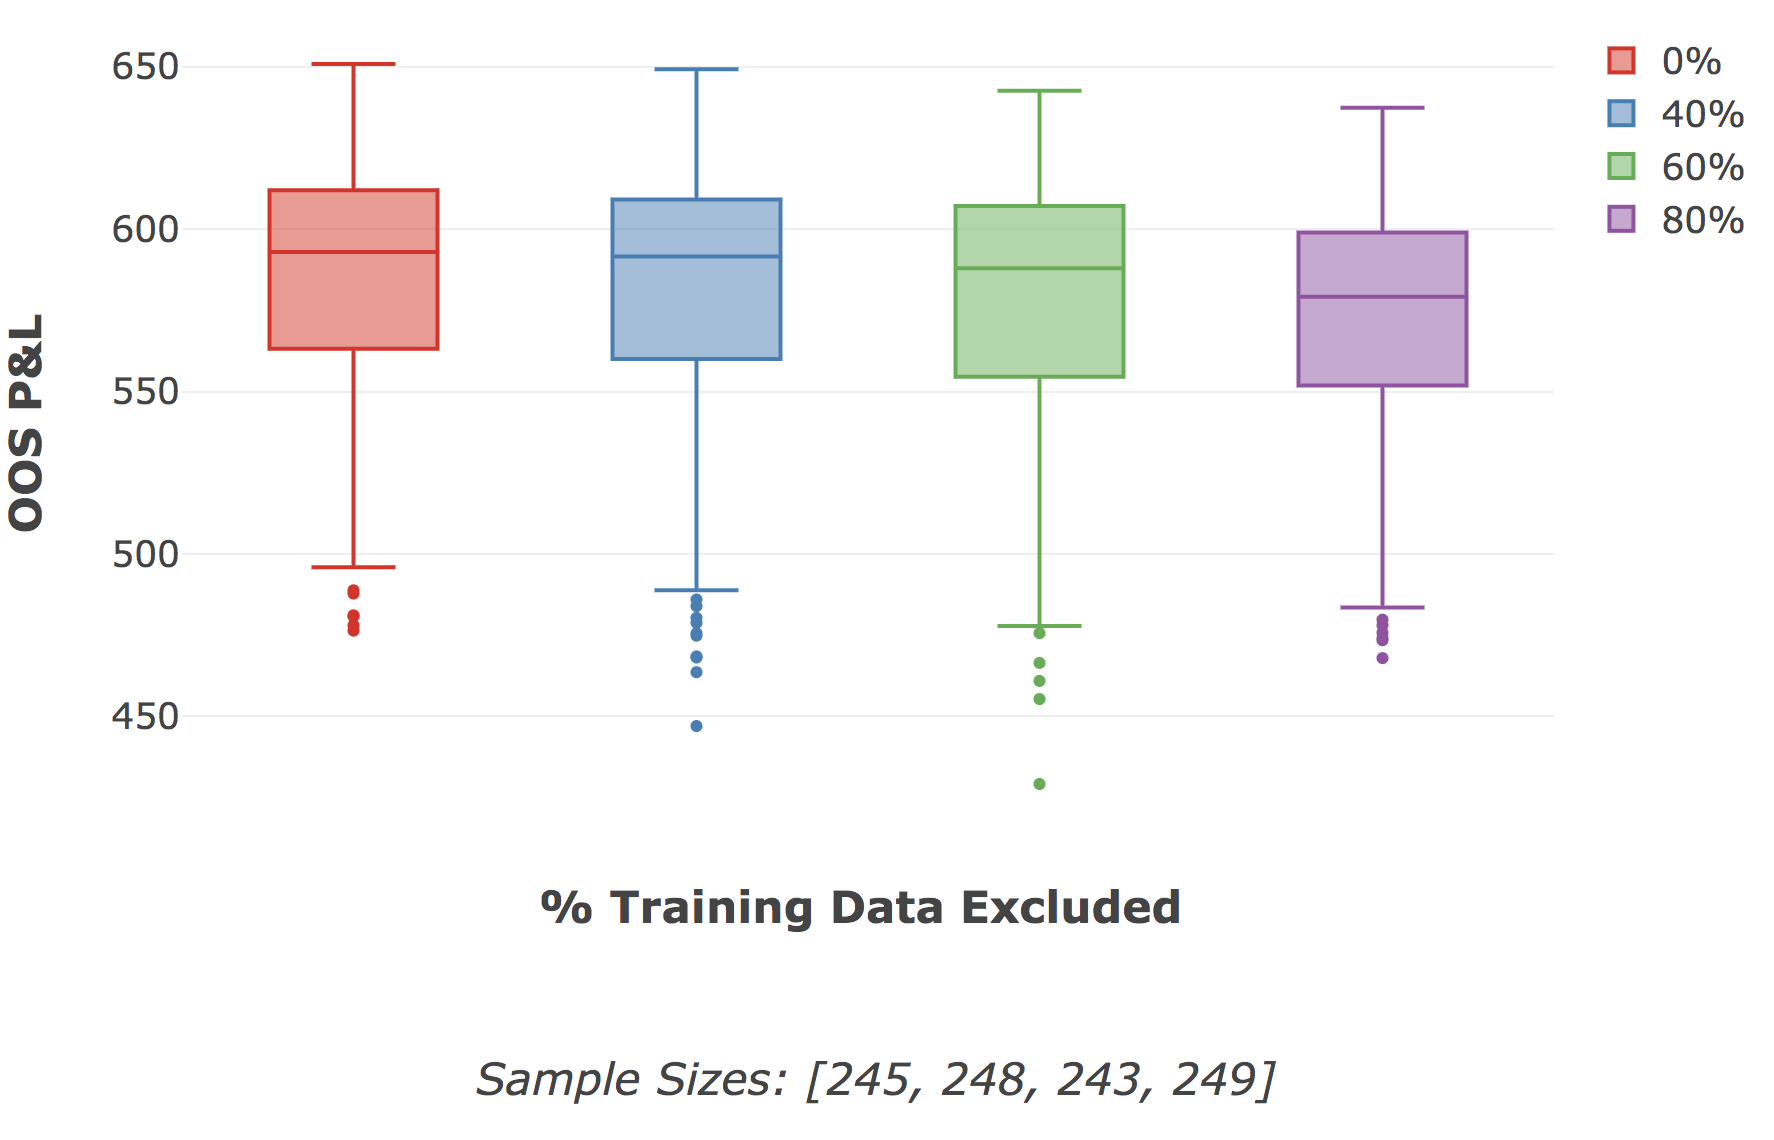
\includegraphics[scale=0.3]{images/results/data/training_data_excluded.png}
	\caption{
		Dataset: Actual10 dataset (\ref{dataset_actual10}), Configuration (some samples with 0 P\&L were excluded for more effective visualization)
		\newline To further explore the effect of IS training on historical data, configurations were run with a percentage of the usual trianing data excluded, with the P\&L results grouped above. It is very interesting to note that the exclusion of up to 80\% of the IS training data resulted in only a 2.2\% drop in median P\&L for those networks. The training in these instances were not adjusted to increase the number of epochs according to the size of IS data, and so the configurations with more data excluded were also in essence trained less. These results, combined with those in Figure \ref{figure-results_pl_max_epochs} show the limited use in training on historical data, and hence the far greater value in current cross sectional information.}
	\label{figure-results_it3_validationset}
\end{figure}


\newpage

\subsection{Probability of Backtest Overfitting}

\subsubsection{Concerns Regarding the PBO Calculation}\label{results_pboconcerns}

The CSCV and PBO techniques, as detailed in \ref{imp_cscv}, were developed by Bailey et al. \cite{BailyPBO} in order to offer a robust methodology of assessing whether a selected strategy is likely to have been justified through backtest overfitting, a common and problematic phenomenon (as discussed in \ref{lr_backtesting}). The crux of the methodology lies on the idea that for overfitting to occur, the strategies that deliver the best IS performance will systematically underperform in the OOS datasets (thus reflecting the model having overfit to the IS noise).\newline

Their methodology offers several key benefits:
\begin{itemize}
	\item[1] The CSCV methodology is generic, model-free and nonparametric, allowing it to arguably used in any model case
	\item[2] There is no requirement of a hold-out set, which removes potential credibility issues reagrding whether the holdout set was treated appropriatley or not
	\item[3] While the Sharpe Ratio is the typically chosen performance metric, the technique is generic enough to allow any performance measure to be used
	\item[4] The logit distribution developed through the assessment offers a useful view on the robustness of the strategies used and the nature of the PBO score
\end{itemize}

\texttt{}\newline
While the methodology is in substance a model free approach to assessing overfitting, the application in a machine learning context has highlighted some shortfalls and dynamics that are worth considering in its usage. Conceptually, overfitting occurs from model parameters being applied to the IS set which perform poorly OOS. For an online learning neural network though, the model parameters which are applied IS for prior training are not necessarily the same parameters that are used for the OOS results (i.e. one may not use the same learning rates for IS SGD training as for OOS OGD training). Further, the parameters of a neural network model are for the most part the weights of the network, which change and adapt during the online learning (OOS) phase. This is the primary strength of the model - while it may very well be overfit to the IS data, an effective learning implementation will result in the model adapting relatively quickly and so move out of the overfit solution space (as seen in \todo{add ref here to low max epochs results}?). Notably, this behaviour would not occur in many static financial econometric models that might typically be more closely associated with backtest overfitting issues.

\texttt{}\newline
The use of the logit metric in the CSCV method also creates some potentially problematic issues due to its basis in an ordinal ranking, and whether the best strategy in the IS set is higher than the median in the OOS set. The effect is that strategies which perform poorly both in the IS and OOS datasets are able to artificially bolster the ordinal position of the best strategy such that it is past the median point and does not result in an increased likelihood of overfitting. As the authors correctly noted, the addition of trials that are doomed to fail will bias results, and if configurations are obviously flawed then they shouldn't have been tried in the first place. In practice though, the issue is more pervasive than suggested. The combinatorial grid search approach as outlined in \todo{add ref here} results in certain parameter combinations that cause networks to perform very poorly. Individually, these parameters may work well in other combinations though, and so there would be no obvious reason to exclude them to begin with. In this sense, an honest search of the solution space where there is no prior knowledge about what will work OOS may result in a PBO score that is lower than it should be. This dynamic is concerning in that it is easy to create poor performance models and so allows the PBO method to be used fraudulently, but is even more so in the case where it might occur without the researcher realising. 

\texttt{}\newline
Another potential implementation concern with CSCV and PBO is the choice of the $S$ parameter, which is the number of splits for the data to be sampled into. As seen in Figure \ref{figure-PBO_by_Split}, the number of splits can have an overwhelming effect on the PBO score reported for the same data sets and results. This is not a problem if the implementation is done honestly and openly, but does allow for misuse and a potential inability to compare PBO scores. Further, while the authors do provide guidelines for choosing $S$ such that the splits will be representative of trading periods, there is still no clearly defined method of choosing the time spans of these periods. The exponential growth in combinations to be tested as $S$ increases also quickly results in reaching computational resource limits, which may further lead to the choice in $S$ being made according to reasons that are not in line with prioritising the correct PBO score to report. These combination sizes can be seen below in Figure \ref{figure-s_combinations}.

\begin{figure}[H]
	\centering 
	\textbf{PBO Scores by Split Values}
	\includegraphics[scale=0.25]{images/results/pbo/PBO_by_Split.png} 
	\caption{
		\newline The curve here shows the significant impact that the choice in the split parameters has for the PBO score calculated, with a monotonically decreasing score as S increases (these scores were for the same set of results). }
	\label{figure-PBO_by_Split}
\end{figure}

\begin{figure}[H]
	\centering 
	\textbf{Number of CSCV Combinations by Split Value}
	\includegraphics[scale=0.25]{images/results/pbo/combination_sizes.png} 
	\caption{
		\newline The number of combinations that have to be procssed by the CSCV method according to the value of the split parameter ($S$) chosen}
	\label{figure-s_combinations}
\end{figure}


\subsubsection{PBO Results}

The full set of tests run (n = 22392) on the Actual10 (\ref{dataset_actual10}) dataset had a final PBO of 1.6\%, having been run with a split of 16. There were 15 years of data, making it a reasonable choice as the split parameter (which needs to be even). Ideally, the splits would represent shorter periods, but the exponential increase in computational time (as seen in Figure \ref{figure-s_combinations}) made this impractical, and 16 also happens to be the typical choice recommended by the authors. The full logit distribution can be seen below in Figure \ref{figure-results_logits_all}.

\todo{correct vals if needed}

\begin{figure}[H]
	\centering 
	\textbf{Logit Distribution for All Configurations (n=22392)}
	\includegraphics[scale=0.25]{images/results/pbo/all_sets_dist.png} 
	\caption{Dataset: Actual10 (\ref{dataset_actual10}) ; Configurations )
		\newline The CSCV logit distribution for all configurations run, with a calculated PBO of 1.6\%.}
	\label{figure-results_logits_all}
\end{figure}


It is of interest to note the dynamics and contribution towards the PBO results. The configuration process went through 2 primary phases: an extremely broad combinatorial grid search, consisting of 20880 configurations; and a second much narrower search of 1512 configurations. Assessing only the configurations from the second phase, results in a PBO score of 6.3\%, which is significantly higher than the overall PBO score, the logit distribution for which can be seen in Figure \ref{figure-results_logits_subset} below. The effect here highlights two important aspects of the PBO calculation:
\begin{itemize}
	\item[1] The scores are much higher for the configurations which were picked more specifically after having already seen a large number of results, which is correctly indicative of increased likelihood to overfit.
	\item[2] However, the PBO score is not monotonically increasing with N, as one would expect. This is counterintuitive and is in line with the concerns raised in \ref{results_pboconcerns} regarding the effects of increasing configuration sample size.
\end{itemize}

\begin{figure}[H]
	\centering 
	\textbf{Logit Distribution for Subset of Configurations (n=1512)}
	\includegraphics[scale=0.25]{images/results/pbo/subset_dist.png} 
	\caption{Dataset: Actual10 (\ref{dataset_actual10}) ; Configurations )
		\newline The CSCV logit distribution for a narrower of configurations run, with a calculated PBO of 6.3\%.}
	\label{figure-results_logits_subset}
\end{figure}


\subsubsection{Framework Success}

While the CSCV and PBO implementations do raise some concerns, the results here do also highlight the efficacy of the framework which has been implemented. The low PBO scores presented here show that the combinatorial search approach combined with an online machine learning model allows researchers to take on a broad exploration of the possible solution space while maintaining a low risk of backtest overfitting, and such that P\&L results which are comparable to the benchmark are achieved, as seen below in section \ref{results_mms}.




\newpage
\subsection{MMS Results}\label{results_mms}.

\subsubsection{Summary of Experiment Results}

\todo{}Add summary here of both distributions, commenting on effect of costs and the 0 network bars.\newline

\begin{figure}[H]
	\centering
	\textbf{OOS P\&L PDF With Benchmark}
	\includegraphics[scale=0.3]{images/results/mms/pl_pdf_nocosts.png} 
	\caption{Dataset: Actual10 (\ref{dataset_actual10}) ; Configurations )
		\newline The PDF of all OOS P\&L values, with the benchmark P\&L indicated in orange.}
	\label{figure-results_pl_pdf}
\end{figure}

\subsubsection{Best Network Results}

\begin{table}[h]
	\centering
	\begin{tabular}{|c|c|c|c|}
		\hline
		\textbf{Measure} &\textbf{Best Network} & \textbf{Benchmark} & \textbf{Difference}\\\hline	
		{Observed P\&L} & {679.03} & {829.72} & {22.19\%} \\\hline
		{Observed P\&L with Costs} & {541.15} & {692.17} & {27.91\%} \\\hline
		{Observed Return Rate} & {2.49\%} & {3.04\%} & {22.48\%} \\\hline
		{Observed Return Rate with Costs} & {1.97\%} & {2.53\%} & {28.21\%} \\\hline
	\end{tabular}
	\newline\newline
	\caption{Best Network vesus Benchmark}\label{tab_bestvsbenchmark}
\end{table}

\begin{table}[h]
	\centering
	\begin{tabular}{|c|c|c|}
		\hline
		\textbf{} &\textbf{Best: No Trade} & \textbf{Best: Trade} \\\hline	
		{Benchmark: No Trade} & {6172} & {1535} \\\hline
		{Benchmark: Trade} & {1546} & {6297} \\\hline
	\end{tabular}
	\newline\newline
	\caption{Best Network vesus Benchmark}\label{tab_best_confusion}
\end{table}

\newpage
\subsection{Results Summary}









\newpage
\section{Conclusions}\label{Conclusion}


\newpage
\section{Appendix}\label{Appendix}

\subsection{Additional Results}

\subsubsection{Additional Results for Section \ref{results_activations_scaling} - Activation Functions and Scaling }\label{results_activations_appendix}

\begin{figure}[H]
	\centering 
	\textbf{SAE: Leaky ReLU vs ReLU (Sythnetic Data)} 
	\includegraphics[scale=0.28]{images/results/activations/synthetic_mse_leakyrelu.png}
	\caption{Dataset Synthetic6  (\ref{dataset_synthetic6}) ; Configuration 
		\newline The plot above shows the SAE MSE, grouped by encoding size and activations, showing a marginal increase in performance for Leaky ReLU activations. }
	\label{figure-synthetic_mse_leakyrelu}
\end{figure}

\subsubsection{Additional Results for Section \ref{results_init} - Weight Initialization Techniques }

\begin{figure}[H]
	\centering 
	\textbf{Prediction Accuracy by Training Epochs (MNIST Data)} 
	\includegraphics[scale=0.28]{images/results/newinit/rbm_pretraining.png}
	\caption{The plot above shows the prediction accuracy achieved on the MNIST dataset according to the number of pre-training epochs using the RBM greedy layerwise methodology as per section \ref{imp_rbm}. There's a clear indication that pre-training allows the network to achieve much higher accuracy much quicker.}
	\label{figure-rbm_pretraining}
\end{figure}

\subsubsection{Additional Results for Section \ref{results_reduction} - Feature Selection }

\begin{figure}[H]
	\centering 
	\textbf{P\&L By Feature Reduction Encoding Layer Size: AGL}
	\includegraphics[scale=0.35]{images/iteration_five/it5_encoding_size_agl.png} 
	%\includegraphics[scale=0.35]{images/iteration_five/it5_sae_init_agl.png}
	\caption{Dataset: AGL (\ref{dataset_agl}) ; Configurations 3 \& 4 (\ref{config3}, \ref{config4}) 
		\newline This figure shows the effects of the difference encoding layer sizes on the P\&L when the relevant SAE is used for the predictive FFN, as for the AGL dataset (with an input of 3 features). Performance for both sizes are similar, though increasing the number of assets may result in a different effect being seen.}
	\label{figure-results_encoding_agl}
\end{figure}

\subsubsection{Additional Results for Section \ref{results_network} - Network Structure and Training }\label{results_network_appendix}

\begin{figure}[H]
	\centering 
	\textbf{MSE By Network Sizes (Actual Data)}
	\includegraphics[scale=0.25]{images/results/network/actual_sae_mse_box.png} 
	\caption{Dataset: Actual10 (\ref{dataset_actual10}) ; Configurations 
		\newline This figure shows the MSE achieved by SAE networks with the indicated sizes, showing a general increase in performance as both layers and layer sizes increase. The network sizes here indicate the final $N$ layers for the SAE, rather than the $2N + 1$ that are present in training. Training parameters such as number of SGD epochs were not adjusted for network size, and so some smaller networks achieved higher performance as they had more accomodating training. The general trends should be focused on as the indicator for more tailored training. As noted in \ref{results_network}, the more typical structure of SAEs with descending layer sizes did not show better performance.}
	\label{figure-actual_sae_mse_box}
\end{figure}

\begin{figure}[H]
	\centering 
	\textbf{MSE By Network Sizes (Synthetic Data)}
	\includegraphics[scale=0.25]{images/results/network/synth_mse_box.png} 
	\caption{Dataset: Synthetic10 (\ref{dataset_synthetic10}) ; Configurations 
		\newline This figure shows the MSE achieved by networks with the indicated sizes, showing a general increase in performance as both layers and layer sizes increase. The network sizes here indicate the final $N$ layers for the SAE, rather than the $2N + 1$ that are present in training. Training parameters such as number of SGD epochs were not adjusted for network size, and so some smaller networks achieved higher performance as they had more accomodating training. The general trends should be focused on as the indicator for more tailored training. As noted in \ref{results_network}, the more typical structure of SAEs with descending layer sizes did not show better performance.}
	\label{figure-synth_mse_box}
\end{figure}

\begin{figure}[H]
	\centering 
	\textbf{P\&L By Network Sizes (Actual Data)}
	\includegraphics[scale=0.3]{images/results/network/actual_pl_box.png} 
	\caption{Dataset: Actual10 (\ref{dataset_actual10}) ; Configurations 
		\newline This figure shows the P\&L achieved by networks with the indicated sizes, showing a general increase in performance as both layers and layer sizes increase. Networks that suffered from exploding ReLU's (and hence have approximately 0 P\&L) have been excluded for the more effective visualization. Training parameters such as number of SGD epochs were not adjusted for network size, and so some smaller networks achieved higher performance as they had more accomodating training. The general trends should be focused on as the indicator for more tailored training.}
	\label{figure-results_actual_pl_box}
\end{figure}

\begin{figure}[H]
	\centering 
	\textbf{P\&L By Network Sizes (Synthetic Data) (Sythetic Data)}
	\includegraphics[scale=0.3]{images/results/network/synth_pl_box.png} 
	\caption{Dataset: Synthetic10 (\ref{dataset_synthetic10}) ; Configurations 
		\newline This figure shows the P\&L achieved by networks with the indicated sizes, showing a general increase in performance as both layers and layer sizes increase. Networks that suffered from exploding ReLU's (and hence have approximately 0 P\&L) have been excluded for the more effective visualization. Training parameters such as number of SGD epochs were not adjusted for network size, and so some smaller networks achieved higher performance as they had more accomodating training. The general trends should be focused on as the indicator for more tailored training.}
	\label{figure-results_synth_pl_box}
\end{figure}

\begin{figure}[H]
	\centering 
	\textbf{SAE MSE by Learning Rate Epoch Cycles (Sythetic Data)}
	\includegraphics[scale=0.3]{images/results/network/lr/synth_mse_lr_epochs.png} 
	\caption{Dataset: Synthetic10 (\ref{dataset_synthetic10}) ; Configurations 
		\newline The SAE networks didn't show significant differences according to the epoch cycles. As discussed in sections \ref{results_gbm_data} and \ref{results_data_hist}, the structure of synthetic data for SAE replication is structurally less complex, and so learning optimizations are less likely to produce large differences.}
	\label{figure-synth_mse_lr_epochs}
\end{figure}

\begin{figure}[H]
	\centering 
	\textbf{Predictive P\&L by OGD Learning Rate (Sythetic Data)}
	\includegraphics[scale=0.3]{images/results/network/lr/synth_ogd_lr.png} 
	\caption{Dataset: Synthetic10 (\ref{dataset_synthetic10}) ; Configurations 
		\newline The networks trained on Synthetic data showed a sharp P\&L increase as the OGD learning rate increased. It wasn't tested if they would experience the same turning point and begin to degrade as seen in networks for Actual data in \ref{results_lr}}.
	\label{figure-synth_ogd_lr}
\end{figure}

\begin{figure}[H]
	\centering 
	\textbf{Predictive P\&L by L1 Regularization  (Sythetic Data)}
	\includegraphics[scale=0.3]{images/results/network/reg/synth_pl_reg.png} 
	\caption{Dataset: Synthetic10 (\ref{dataset_synthetic10}) ; Configurations 
		\newline }.
	\label{figure-synth_pl_reg}
\end{figure}













\newpage
\subsection{Configuration Sets Used}

\subsubsection{Configuration1 - SAE}\label{config1}

\begin{itemize}
	\item Data: Closing Prices for ACL, AGL, AMS, AOD, BAW, BIL, BVT, CFR, CRH, DDT
	\item Data Windows: 1, 5, 20 (thus input of 30)
	\item Data Scaling: Normalize, Standardize
	\item Weight Init,: Xavier Glorot Uniform
	\item All Layer Encodings: Sigmoid, ReLU, Linear (split by hidden, encoding and output)
	\item Encoding Layer Size: 5, 15, 25
	\item Hidden Layer Size: 60, 120
	\item Number of Hidden Layers: 1, 2, 3
	\item Learning Rates: Various for each different activation type (chosen by hidden activation used)
\end{itemize}

\subsubsection{Config2 - Predictive FFN}\label{config2}

\begin{itemize}
	\item SAEs: Best performance (lowest MSE) of encoding sizes 3, 6, 9, 12, 15 (input 18) from Config1, of both Limited Scaling and typical Scaling methods
	\item Output Activations: ReLU, Linear
	\item Hidden Activations: ReLU, Linear
	\item Layer Sizes: 40, 80
	\item Number of Layers: 1, 3
	\item Various Learning rates for SGD \& OGD training
\end{itemize}

\subsubsection{Configuration3 - SAE}\label{config3}
\begin{itemize}
	\item Data Windows: [1,5,20], [5,20,60], [10,20,60]
	\item Data Scaling: Normalize
	\item Weight Init: Xavier Glorot Uniform, He, DC
	\item Layer Encodings: Leaky ReLU with Linear encoding and output
	\item Encoding Layer Size: 1, 2
	\item Network Sizes: (12,6), (12), (12,12), (12,9), (9,6), (9,6,3),(12,6,3), (9,9,9), (9,9)
	\item Learning Rates: Scheduled from (0.005, 0.01, 0.05, 0.1) to 0.0001
	\item Learning Rate Epoch Schedules: (100,300)
	\item SGD Epochs: 400
	\item Minibatch Size: 20
	\item SAE Validation Split: (0.8)
\end{itemize}
	
\subsubsection{Configuration4 - Predictive FFN}\label{config4}
\begin{itemize}
	\item SAEs: Best networks by encoding size and data aggegations from Configuration3.
	\item Data Windows: [1,5,20], [5,20,60], [10,20,60]
	\item Data Scaling: Normalize
	\item Weight Init: Xavier Glorot Uniform, He, DC
	\item Layer Encodings: Leaky ReLU with Linear output
	\item Network Sizes: (12, 12), (12, 12, 12), (12, 9, 9, 6), (12, 9, 6), (12)
	\item Learning Rates: Scheduled from (0.01, 0.05, 0.1) to 0.0001
	\item Learning Rate Epoch Schedules: (100)
	\item SGD Epochs: 400
	\item Minibatch Size: 20
	\item Training Validation Split: (1.0) (i.e. none)
	\item OGD Learning Rates: (0.01, 0.05)
	\item L1 Regularization: (0, 0.1)
\end{itemize}


\subsubsection{Configuration5 - SAE}\label{config5}


\begin{itemize}
	\item Data Windows: [1,5,20], [5,20,60], [10,20,60]
	\item Learning Rate Schedules: 0.005 to (0.01, 0.05, 0.1) by (100) epochs
	\item Network Sizes:(120, 60, 30), (90, 60, 30), (90, 90, 90), (90, 90), (120, 90), (120,60), (120)
	\item Encoding: 25;20;15;10;5
	\item SGD Epochs: 400
	\item Minibatch Size: 20
	\item SAE Validation Split: (0.8)
	\item Weight Init: Xavier Glorot Uniform, He, DC
	\item Layer Encodings: Leaky ReLU with Linear encoding and output
	
\end{itemize}

\subsubsection{Configuration6 - Predictive FFN}\label{config6}

\begin{itemize}
	\item Best SAEs by encoding size and window aggregations (15 total) from Configuration5
	\item Learning Rate Schedules: 0.005 to (0.01, 0.05, 0.1) by (100) epochs
	\item Network Structures: (120;120;120;120), (120,90,90,60), (120,90,60),(120,120,120),(120,120),(120,60),(120)
	\item OGD Learning Rates: (0.01, 0.05)
	\item Data Windows: [1,5,20], [5,20,60], [10,20,60]
	\item Data Scaling: Normalize
	\item Weight Init: Xavier Glorot Uniform, He, DC
	\item Layer Encodings: Leaky ReLU with Linear output
	\item Learning Rate Epoch Schedules: (100)
	\item SGD Epochs: 400
	\item Minibatch Size: 20
	\item Training Validation Split: (1.0) (i.e. none)
	\item L1 Regularization: (0, 0.1)
\end{itemize}

\subsubsection{Configuration7 - SAE}\label{config7}

\begin{itemize}
	\item Data: Closing prices for AGL \& ACL
	\item Processing: Time windows of 1, 5 and 20 (thus an input vector of size 6)
	\item Encoding Layer Activations: Sigmoid and Linear
	\item Encoding Layer Size: 5
	\item Hidden Layer Size: 15
	\item Number of Hidden Layers: 1, 2
	\item Learning Rates: 0.0000001, 0.00001, 0.001, 0.1, 1.0, 2.0
\end{itemize}

\newpage
\begin{thebibliography}{bibliography}

\bibitem{Albers}
Albers S. Online Algorithms: a survey. Mathematics Subject Classification (1991): 68W25, 
68W40. Available at: https://link.springer.com/content/pdf/10.1007%2Fs10107-003-0436-0.pdf

\bibitem{Aparicio}
Aparicio, Diego and Lopez de Prado, Marcos, How Hard Is It to Pick the Right Model? (December 2017). Available at SSRN: https://ssrn.com/abstract=3044740 or http://dx.doi.org/10.2139/ssrn.3044740

\bibitem{Arthur}
B. Arthur (1995) Complexity in Economics and Financial Markets, Complexity 1 (1), 20???25.

\bibitem{BailyPBO}
Bailey, David H. and Borwein, Jonathan and Lopez de Prado, Marcos and Zhu, Qiji Jim, The Probability of Backtest Overfitting (February 27, 2015). Journal of Computational Finance (Risk Journals), 2015, Forthcoming. Available at SSRN: https://ssrn.com/abstract=2326253 or http://dx.doi.org/10.2139/ssrn.2326253

\bibitem{BaileyBTL}
Bailey, David H. and Borwein, Jonathan and Lopez de Prado, Marcos and Zhu, Qiji Jim, Pseudo-Mathematics and Financial Charlatanism: The Effects of Backtest Overfitting on Out-of-Sample Performance (April 1, 2014). Notices of the American Mathematical Society, 61(5), May 2014, pp.458-471. Available at SSRN: https://ssrn.com/abstract=2308659 or http://dx.doi.org/10.2139/ssrn.2308659

\bibitem{BaileySharpe}
Bailey, David H. and Lopez de Prado, Marcos, The Deflated Sharpe Ratio: Correcting for Selection Bias, Backtest Overfitting and Non-Normality (July 31, 2014). Journal of Portfolio Management, 40 (5), pp. 94-107. 2014 (40th Anniversary Special Issue).. Available at SSRN: https://ssrn.com/abstract=2460551 or http://dx.doi.org/10.2139/ssrn.2460551

\bibitem{Bakiri}
G. Bakiri and T. G. Dietterich. Achieving high-accuracy text-to-speech with machine learning. In R. I. Damper, editor, Data Mining Techniques in Speech Synthesis. Chapman and Hall, New York, NY, 2002. 22

\bibitem{Bao}
Bao W, Yue J, Rao Y (2017) A deep learning framework for financial time series using stacked autoencoders and long-short term memory. PLoS ONE 12(7): e0180944. https://doi.org/10.1371/journal.pone.0180944

\bibitem{Bartlett}
Bartlett P., Hazan E. Adaptive Online Gradient Descent. Available at: http://papers.nips.cc/paper/3319-adaptive-online-gradient-descent.pdf

\bibitem{Bengio1}
Yoshua Bengio, Pascal Lamblin, Dan Popovici, and Hugo Larochelle. Greedy layer-wise training of deep networks. In Bernhard Scholkopf, John Platt, and Thomas Hoffman, editors, ¨ Advances in Neural Information Processing Systems 19 (NIPS’06), pages 153–160. MIT Press, 
2007. Available at: http://papers.nips.cc/paper/3048-greedy-layer-wise-training-of-deep-networks.pdf

\bibitem{Bengio2}
Bengio, Yoshua, and Samy Bengio. "Modeling high-dimensional discrete data with multi-layer neural networks." Advances in Neural Information Processing Systems. 2000.
Available at: http://papers.nips.cc/paper/1679-modeling-high-dimensional-discrete-data-with-multi-layer-neural-networks.pdf

\bibitem{Bengio3}
Bengio, Yoshua, Aaron Courville, and Pascal Vincent. "Representation learning: A review and new perspectives." IEEE transactions on pattern analysis and machine intelligence 35.8 (2013): 1798-1828.
Available at: https://ieeexplore.ieee.org/stamp/stamp.jsp?tp=\&arnumber=6472238\&tag=1

\bibitem{Bottou}
Bottou L., Le Cun Y. Large Scale Online Learning. Available at: http://papers.nips.cc/paper/2365-large-scale-online-learning.pdf

\bibitem{Bottou2}
Bottou, L. and Murata, N. (2002). Stochastic Approximations and Efficient Learning. In Arbib, M. A., editor, The Handbook of Brain Theory and Neural Networks, Second edition,. The MIT Press, Cambridge, 

\bibitem{Ciresan}
Cireşan, Dan Claudiu, et al. "Deep, big, simple neural nets for handwritten digit recognition." Neural computation 22.12 (2010): 3207-3220.
Available at: \url{https://www.mitpressjournals.org/doi/abs/10.1162/NECO_a_00052}

\bibitem{Chu}
Chu C., Time series segmentation: A sliding window approach. Information Sciences, Volume 85, Issues 1–3, July 1995, Pages 
147-173. Available at: \url{ttps://www.sciencedirect.com/science/article/pii/002002559500021G#!}

\bibitem{Chung}
 F. L. Chung, T. C. Fu, R. Luk, and V. Ng, “Flexible time series pattern matching based on perceptually important points,’’ in Proc. Int. Joint Conf. Artificial Intelligence Workshop  
 Learning from Temporal and Spatial Data in International Joint Conference on Artificial Intelligence (IJCAI'01), Seattle, Washington, USA, 4-10 August, 2001, p. 
 1-7. Available at: http://hdl.handle.net/10397/48578

\bibitem {Crutchfield}
J. P. Crutchfield, (2011), Between order and chaos, Nature Physics, Vol. 8, January 2012, 17-23

\bibitem{Dauphin}
Dauphin, Y. et al. Identifying and attacking the saddle point problem in high-dimensional non-convex optimization. In Proc. Advances in Neural Information Processing Systems 27 2933–2941 (2014)
Available at: http://papers.nips.cc/paper/5486-identifying-and-attacking-the-saddle-point-problem-in-high-dimensional-non-convex-optimization 

\bibitem{Devarakonda}
Aditya Devarakonda, Maxim Naumov \& Michael Garland. ADABATCH: ADAPTIVE BATCH SIZES FOR TRAINING
DEEP NEURAL NETWORKS. Available at: https://arxiv.org/pdf/1712.02029.pdf

\bibitem{Donoho}
David L. Donoho, High-Dimensional Data Analysis: The Curses and Blessings of 
Dimensionality (August 8, 2000). Available at: \url{http://citeseerx.ist.psu.edu/viewdoc/download?doi=10.1.1.329.3392&rep=rep1&type=pdf}

\bibitem{Duchi}
John Duchi, Elad Hazan and Yoram Singer. Adaptive Subgradient Methods for
Online Learning and Stochastic Optimization. Journal of Machine Learning Research 12 (2011) 
2121-2159. Available at: http://www.jmlr.org/papers/volume12/duchi11a/duchi11a.pdf

\bibitem{Erhan}
Erghan D., Bengio Y., Courville A, Manzagol P., Vincent P. Why Does Unsupervised Pre-training Help Deep 
Learning?, Journal of Machine Learning Research 11 (2010) 625-660 . Available 
at: http://www.jmlr.org/papers/volume11/erhan10a/erhan10a.pdf

\bibitem{Fama}
E.F. Fama, The behavior of stock-market prices, J. Bus., 1 (1965), pp. 34-105. 
Available at: https://doi.org/10.1086/294743

\bibitem{Fan1}
Jianqing Fan, Runze Li, 
Statistical Challenges with High Dimensionality: Feature Selection in Knowledge Discovery 
(7 Feb, 2006). Available at: https://arxiv.org/abs/math/0602133

\bibitem{Fan2}
Fan, J., \& Fan, Y. (2008). High Dimensional Classification Using Features Annealed Independence Rules. Annals of Statistics, 36(6), 2605–2637. http://doi.org/10.1214/07-AOS504

\bibitem {Ge}
Ge, Rong, et al. "Escaping from saddle points—online stochastic gradient for tensor decomposition." Conference on Learning Theory. 2015.
Available at: http://proceedings.mlr.press/v40/Ge15.pdf 

\bibitem{Goodfellow}
Goodfellow, Ian J., et al. "Maxout networks." arXiv preprint arXiv:1302.4389 (2013).
Available at: http://proceedings.mlr.press/v28/goodfellow13.pdf

\bibitem{Glorot}
Glorot, Xavier, and Yoshua Bengio. "Understanding the difficulty of training deep feedforward neural networks." Proceedings of the thirteenth international conference on artificial intelligence and statistics. 2010.
Available at: http://proceedings.mlr.press/v9/glorot10a/glorot10a.pdf

\bibitem{Glorot2}
Glorot, Xavier, Antoine Bordes, and Yoshua Bengio. "Deep sparse rectifier neural networks." Proceedings of the Fourteenth International Conference on Artificial Intelligence and Statistics. 2011.
Available at: http://proceedings.mlr.press/v15/glorot11a/glorot11a.pdf 

\bibitem{Griffioen} 
Griffioen, Gerwin A. W., Technical Analysis in Financial Markets (March 3, 2003).

\bibitem{Hansen}
Hansen, Peter Reinhard and Lunde, Asger and Nason, James M., The Model Confidence Set (March 18, 2010). Available at SSRN: https://ssrn.com/abstract=522382 or http://dx.doi.org/10.2139/ssrn.522382

\bibitem{Harvey}
Harvey, Campbell R. and Liu, Yan, Backtesting (July 28, 2015). Available at SSRN: https://ssrn.com/abstract=2345489 or http://dx.doi.org/10.2139/ssrn.2345489

\bibitem{Hawkins}
Hawkins, Douglas. (2004). The Problem of Overfitting. Journal of chemical information and computer sciences. 44. 1-12. 10.1021/ci0342472. 

\bibitem{He}
Kaiming He,  Xiangyu Zhang,  Shaoqing Ren,  Jian Sun. Delving Deep into Rectifiers: Surpassing Human-Level Performance on ImageNet Classification. Available at: https://arxiv.org/pdf/1502.01852.pdf

\bibitem{Hinton1}
Geoffrey E. Hinton, Simon Osindero, and Yee Whye Teh. A fast learning algorithm for deep belief nets. Neural Computation, 18:1527–1554, 2006. 
Available at: https://www.mitpressjournals.org/doi/abs/10.1162/neco.2006.18.7.1527

\bibitem{Hinton2}
G. E. Hinton, R. R. Salakhutdinov, Reducing the Dimensionality of Data with Neural 
Networks. Science  28 Jul 2006: Vol. 313, Issue 5786, pp. 504-507 DOI: 
10.1126/science.1127647. Available at: http://science.sciencemag.org/content/313/5786/504/tab-pdf

\bibitem{Hinton3}
Geoffrey E. Hinton, Training Products of Experts by Minimizing Contrastive Divergence,Neural Computation
Volume 14 | Issue 8 | August 2002  p.1771-1800 . Available at: https://www.mitpressjournals.org/doi/pdf/10.1162/089976602760128018

\bibitem{Hinton4}
Hinton, Geoffrey E., et al. "Improving neural networks by preventing co-adaptation of feature detectors." arXiv preprint arXiv:1207.0580 (2012).
Available at: https://arxiv.org/pdf/1207.0580.pdf

\bibitem{Hinton5}
Geoffrey E. Hinton, A Practical Guide to Training Restricted Boltzmann Machines, August 2, 2010. Available at: http://learning.cs.toronto.edu

\bibitem{HLZ}
Campbell R. Harvey \& Yan Liu \& Heqing Zhu, 2016. "… and the Cross-Section of Expected Returns," Review of Financial Studies, vol 29(1), pages 5-68.

\bibitem{Hochreiter}
Sepp Hochreiter,  Jürgen Schmidhuber. Long Short-Term Memory. Neural Computation Volume 9 | Issue 8 | November 15, 1997  
p.1735-1780. Available at https://www.mitpressjournals.org/doi/abs/10.1162/neco.1997.9.8.1735.

\bibitem {Hornik}
K. Hornik, Multilayer feed-forward networks are universal approximators, Neural Networks, vol 2, 1989

\bibitem{Hsu}
Hsu D. Time Series Compression Based on Adaptive Piecewise
Recurrent Autoencoder (17 August 2017). Available at: https://arxiv.org/pdf/1707.07961.pdf

\bibitem{Ivakhnenko}
Ivakhnenko, A. G. (1971). Polynomial theory of complex systems. IEEE Transactions
on Systems, Man and Cybernetics, (4), 364–378. Available at: https://ieeexplore.ieee.org/document/4308320/

\bibitem{ImageNet}
Krizhevsky, Alex, Ilya Sutskever, and Geoffrey E. Hinton. "Imagenet classification with deep convolutional neural networks." Advances in neural information processing systems. 2012.
Available at: http://papers.nips.cc/paper/4824-imagenet-classification-with-deep-convolutional-neural-networks

\bibitem{Ioannidis} 
Ioannidis JPA (2005) Why Most Published Research Findings Are False. PLoS Med 2(8): e124. https://doi.org/10.1371/journal.pmed.0020124

\bibitem {Johnson}
N. Johnson, G. Zhao, E. Hunsader, H. Qi, N. Johnson, J. Meng \& Brian Tivnan (2013). Abrupt rise of new machine ecology beyond human response time. Sceintific Reports 3(2627). DOI: 10.1038/srep02627

\bibitem{Kahn}
Kahn, Michael N. . Technical Analysis Plain and Simple: Charting the Markets in Your Language, Financial Times Press, Upper Saddle River, New Jersey, p. 9. ISBN 0-13-134597-4.(2006)

\bibitem{Knerr}
Stefan Knerr, Handwritten Digit Recognition by Neural Networks with Single-Layer 
Training. 962 IEEE TRANSACTIONS ON NEURAL NETWORKS, VOL. 3, NO. 6, NOVEMBER 
1992. Available at: \url{https://ieeexplore.ieee.org/stamp/stamp.jsp?tp=&arnumber=165597 }


\bibitem{Langford}
John Langford, Lihong Li and Tong Zhang. Sparse Online Learning via Truncated 
Gradient. Journal of Machine Learning Research 10 (2009) 777-801 Submitted 6/08; Revised 11/08; Published 
3/09. Available at: http://www.jmlr.org/papers/volume10/langford09a/langford09a.pdf 

\bibitem{Langkvist}
Martin Längkvist, Lars Karlsson,  Amy Loutfi, A review of unsupervised feature learning and deep learning for time-series 
modeling, Applied Autonomous Sensor Systems, School of Science and Technology, Örebro University, SE-701 82 Örebro, 
Sweden. Available at: \url{https://www.sciencedirect.com/science/article/pii/S0167865514000221#bi005}

\bibitem{LeCun}
LeCun Y., Bottou L, Orr G, Muller K. Efficient Backprop. Available at: http://yann.lecun.com/exdb/publis/pdf/lecun-98b.pdf

\bibitem{LeCun2}
LeCun, Y. (1988). A theoretical framework for back-propagation. In D. Touretzky,
G. Hinton, \& T. Sejnowski (Eds.), Proceedings of the 1988 connectionist models summer school (pp. 21–28).
\url{Available at: https://www.researchgate.net/profile/Yann_Lecun/publication/2360531_A_Theoretical_Framework_for_Back-Propagation/links/0deec519dfa297eac1000000/A-Theoretical-Framework-for-Back-Propagation.pdf}

\bibitem{LeCun3}
LeCun, Y., Boser, B., Denker, J. S., Henderson, D., Howard, R. E., Hubbard, W., et al.
(1989). Back-propagation applied to handwritten zip code recognition. Neural
Computation, 1(4), 541–551. Available at: http://papers.nips.cc/paper/293-handwritten-digit-recognition-with-a-back-propagation-network.pdf

\bibitem{LeCun4}
Yann LeCun, Yoshua Bengio \& Geoffrey Hinton. Deep learning, Nature volume 521, pages 436–444 (28 May 
2015). Available at: https://www.nature.com/articles/nature14539

\bibitem{LeRoux}
Le Roux, Nicolas, and Yoshua Bengio. "Representational power of restricted Boltzmann machines and deep belief networks." Neural computation 20.6 (2008): 1631-1649.
Available at: http://www.iro.umontreal.ca/~lisa/publications2/index.php/attachments/single/22

\bibitem{Liu}
Liu X., Lin Z., Wang H. Novel Online Methods for Time Series Segmentation.  IEEE TRANSACTIONS ON KNOWLEDGE AND DATA ENGINEERING, VOL. 20, NO. 12, DECEMBER 
2008. Available at: \url{https://ieeexplore.ieee.org/stamp/stamp.jsp?arnumber=4445667&tag=1}

\bibitem{Lo}
Lo, Andrew W., The Statistics of Sharpe Ratios. Financial Analysts Journal, Vol. 58, No. 4, July/August 2002. Available at SSRN: https://ssrn.com/abstract=377260

\bibitem{Loshchilov}
Ilya Loshchilov, Frank Hutter, SGDR: Stochastic Gradient Descent with Warm Restarts, ICLR 2017 conference paper. Available at: https://arxiv.org/abs/1608.03983


\bibitem{Lv}
Yisheng Lv, Yanjie Duan, Wenwen Kang, Zhengxi Li, and Fei-Yue Wang. Traffic Flow Prediction With Big Data:
A Deep Learning Approach. IEEE TRANSACTIONS ON INTELLIGENT TRANSPORTATION SYSTEMS, VOL. 16, NO. 2, APRIL 
2015. Available at: \url{https://ieeexplore.ieee.org/stamp/stamp.jsp?tp=&arnumber=6894591&tag=1}

\bibitem{Mahajan}
Mahajan D., Keerthi S., Sundararajan S., Bottou L. A Parallel SGD method with Strong 
Convergence. Available at: https://arxiv.org/pdf/1311.0636.pdf

\bibitem{McLean}
McLean, R. David and Pontiff, Jeffrey, Does Academic Research Destroy Stock Return Predictability? (January 7, 2015). Journal of Finance, Forthcoming. Available at SSRN: https://ssrn.com/abstract=2156623 or http://dx.doi.org/10.2139/ssrn.2156623

\bibitem{Minksy}
M Minsky, SA Papert, L Bottou (1988). Perceptrons: An introduction to computational  geometry. Available at: \url{https://books.google.co.za/books?hl=en&lr=&id=PLQ5DwAAQBAJ&oi=fnd&pg=PR5&dq=Minsky+Papert+1969+%E2%80%94+Perceptrons&ots=zyEDwMvmXX&sig=aVXF7DBJKAOxW066S4UCyzhNARw#v=onepage&q=Minsky%20Papert%201969%20%E2%80%94%20Perceptrons&f=false}

\bibitem{Murphy}
Murphy, John J. Technical analysis of the financial markets: A comprehensive guide to trading methods and applications. Penguin, 1999.

\bibitem{Packard}
Geometry from a Time Series, N. H. Packard, J. P. Crutchfield, J. D. Farmer, and R. S. Shaw. Available at: \url{https://journals.aps.org/prl/pdf/10.1103/PhysRevLett.45.712}

\bibitem{Pascanu}
Pascanu, Razvan, Tomas Mikolov, and Yoshua Bengio. "On the difficulty of training recurrent neural networks." International Conference on Machine Learning. 2013.
Available at: http://proceedings.mlr.press/v28/pascanu13.pdf

\bibitem{Peters}
Ole Peters, Alexander Adamou. "Ergodicity Economics". London Mathematical Laboratory, 2018/06/30. Available at: \url{https://ergodicityeconomics.files.wordpress.com/2018/06/ergodicity_economics.pdf}

\bibitem{Prado}
Lopez de Prado, Marcos, The Future of Empirical Finance (May 31, 2015). Journal of Portfolio Management, 41(4). Summer 2015. Forthcoming.. Available at SSRN: https://ssrn.com/abstract=2609734 or http://dx.doi.org/10.2139/ssrn.2609734

\bibitem{Povey}
Povey D., Zhang X., Khudanpur S. Parallel training of Deep Neural Networks with Natural Gradient and Parameter Averaging. Available at: \url{http://citeseerx.ist.psu.edu/viewdoc/download?doi=10.1.1.745.6995&rep=rep1&type=pdf}

\bibitem{Ranzato1}
Marc’Aurelio Ranzato, Christopher Poultney, Sumit Chopra, and Yann LeCun. Efficient learning of sparse representations with an energy-based model. In B. Scholkopf, J. Platt, and T. Hoffman, ¨ editors, Advances in Neural Information Processing Systems 19 (NIPS’06), pages 1137–1144. MIT Press, 
2007. Aavilable at: http://papers.nips.cc/paper/3112-efficient-learning-of-sparse-representations-with-an-energy-based-model.pdf

\bibitem{Rumelhart}
Rumelhart, D. E., Hinton, G. E., \& Williams, R. J. (1986). Learning internal representations by error propagation. In D. E. Rumelhart, \& J. L. McClelland (Eds.), Parallel distributed processing, vol. 1 (pp. 318–362). MIT Press.

\bibitem{Schaefer}
Robert L. Schaefer (2012) Subset Selection in Regression, Technometrics, 34:2, 229, DOI: 10.1080/00401706.1992.10484917
  
 \bibitem{Schmidhuber}
J Schmidhuber (2015). Deep learning in neural networks: An overview. Neural Networks Volume 61, January 2015, Pages 
85-117. Available at https://www.sciencedirect.com/science/article/pii/S0893608014002135. 
  
\bibitem{Schorfheide}
Schorfheide, Frank, and Kenneth I. Wolpin. 2012. "On the Use of Holdout Samples for Model Selection." American Economic Review, 102 (3): 477-81.

\bibitem {Schwager}
Jack D. Schwager. Getting Started in Technical Analysis, Page 2 (1999)


\bibitem{Sermanet}
Sermanet, Pierre, et al. "Pedestrian detection with unsupervised multi-stage feature learning." Computer Vision and Pattern Recognition (CVPR), 2013 IEEE Conference on. IEEE, 2013.
Available at: https://arxiv.org/abs/1212.0142

\bibitem{Shalev}
Shai Shalev-Shwartz, Yoram Singer, and Nathan Srebro. Pegasos: Primal Estimated sub-GrAdient SOlver for SVM. In Proceedings of the Twenty-Fourth International Conference on Machine Learning (ICML-07), 2007.

\bibitem{Siegelmann}
Siegelmann, H. (1992). Theoretical foundations of recurrent neural networks (Ph.D. thesis), New Brunswick Rutgers, The State of New Jersey: Rutgers. Available at: \url{http://citeseerx.ist.psu.edu/viewdoc/download?doi=10.1.1.38.920&rep=rep1&type=pdf}

\bibitem{Smith}

Smith, Leslie. Cyclical Learning Rates for Training Neural Networks. Available at: \url{https://arxiv.org/abs/1506.01186}

\bibitem {Skabar}
 Skabar, Cloete, Networks, Financial Trading and the Efficient Markets Hypothesis (http://crpit.com/confpapers/CRPITV4Skabar.pdf)

\bibitem{Takeuchi}
Takeuchi L, Lee Y. Applying Deep Learning to Enhance Momentum Trading Strategies in 
Stocks. Technical Report, 2013. Available at: http://www.smallake.kr/wp-content/uploads/2017/04/TakeuchiLee-ApplyingDeepLearningToEnhanceMomentumTradingStrategiesInStocks.pdf

\bibitem{Takens}
Floris Takens, Detecting strange attractors in turbulence. Available at: \url{https://link.springer.com/chapter/10.1007/BFb0091924}

\bibitem{Troiano}
Troiano L., Mejuto E., Kriplani P.On Feature Reduction using Deep Learning
for Trend Prediction in Finance (11 Apr 2017).  Available at: 
https://arxiv.org/abs/1704.03205.

\bibitem{Tseng}
Tseng P., AN INCREMENTAL GRADIENT(-PROJECTION) METHOD
WITH MOMENTUM TERM AND ADAPTIVE STEPSIZE RULE. SIAM J. OPTIM.  Vol. 8, No. 2, pp. 506–531, May 
1998. Available at: https://pdfs.semanticscholar.org/1a29/6a1577478654a54a9f801f93f71b7d853c53.pdf

\bibitem{Vincent}
Vincent P., Larochell H., Lajoie I., Bengio Y., Manzagol P., Stacked Denoising Autoencoders: Learning Useful Representations in
a Deep Network with a Local Denoising Criterion. Journal of Machine Learning Research 11 (2010) 
3371-3408. Available at: http://www.jmlr.org/papers/volume11/vincent10a/vincent10a.pdf

\bibitem{Wan}
Wan Y., Gong X., Si Y. Effect of segmentation on financial time series pattern 
matching. Applied Soft Computing Volume 38, January 2016, Pages 346-359. 
Available at: https://www.sciencedirect.com/science/article/pii/S1568494615006341

\bibitem {Wang}
Linnan Wang,  Yi Yang, Renqiang Min, Srimat Chakradhar. Accelerating deep neural network training with 
inconsistent stochastic gradient descent. Neural Networks
Volume 93, September 2017, Pages 219-229. Available at: https://www.sciencedirect.com/science/article/pii/S0893608017301399

\bibitem{Wang2}
Wang, Sida, and Christopher Manning. "Fast dropout training." international conference on machine learning. 2013.
Available at: http://proceedings.mlr.press/v28/wang13a.pdf

\bibitem{WaveNet}
Van Den Oord, Aaron, et al. "Wavenet: A generative model for raw audio." arXiv preprint arXiv:1609.03499 (2016).
Available at: https://arxiv.org/abs/1609.03499

\bibitem{Wilcox}
Wilcox, Diane and Gebbie, Timothy John, Hierarchical Causality in Financial Economics (August 24, 2014). Available at SSRN: https://ssrn.com/abstract=2544327 or http://dx.doi.org/10.2139/ssrn.2544327

\bibitem{Weiss}
Weiss, S. M, \& Kulikowski, C. A. (1991). Computer systems that learn : classification and prediction methods from statistics, neural nets, machine learning, and expert systems. San Mateo (Calif.): Kaufmann.

\bibitem{Werbos}
Werbos, P. J. (1974). Beyond regression: new tools for prediction and analysis in the behavioral sciences (Ph.D. thesis), Harvard 
University. Available at: \url{https://www.researchgate.net/publication/244947191_1974_Beyond_regression_New_tools_for_predicting_and_analysis_in_the_behavioral_sciences}

\bibitem{Werbos2}
Paul J. Werbos. Applications of advances in nonlinear sensitivity analysis. 
System Modeling and Optimization pp 762-770. Available at: https://link.springer.com/chapter/10.1007/BFb0006203

\bibitem{Wu}
Wu, Huaiqin. "Global stability analysis of a general class of discontinuous neural networks with linear growth activation functions." Information Sciences 179.19 (2009): 3432-3441.
Available at: \url{https://ac.els-cdn.com/S0020025509002539/1-s2.0-S0020025509002539-main.pdf?_tid=fc9d5d20-c0fe-4107-947c-6a4d9e472aab&acdnat=1526319168_bc401e01e4ab496b50b8d568dcafb0b3}

\bibitem{Yin}
Yin J., Si Y., Gong Z. Financial Time Series Segmentation Based On Turning 
Points. Proceedings of 2011 International Conference on System Science and Engineering, Macau, China - June 
2011. Available at: \url{https://ieeexplore.ieee.org/stamp/stamp.jsp?tp=&arnumber=5961935}

\bibitem{Zeiler}
Zeiler M. ADADELTA: An Adaptive Learning Rate Method. Available at: https://arxiv.org/abs/1212.5701

\bibitem{Zinkevich}
Zinkevich M, Weimer M, Smola A, Li L. Parallelized Stochastic Gradient Descent. 
Available at: 
http://papers.nips.cc/paper/4006-parallelized-stochastic-gradient-descent.pdf

\bibitem{Zhao}
Zhao Y., Li J., Yu L. A deep learning ensemble approach for crude oil price 
forecasting.  Available at: https://doi.org/10.1016/j.eneco.2017.05.023

\bibitem{Zhang}
Tong Zhang. Solving large scale linear prediction problems using stochastic gradient descent algorithms. In Proceedings of the Twenty-First International Conference on Machine Learning (ICML-04), pages 919–926, 2004

\bibitem{Zhou}
Zhou B., Hu J. A Dynamic Pattern Recognition Approach Based on Neural Network for Stock Time-Series. 2009 World Congress on Nature \& Biologically Inspired Computing (NaBIC 
2009). Available at:\url{ https://ieeexplore.ieee.org/stamp/stamp.jsp?tp=&arnumber=5393674}

\end{thebibliography}


\end{document}

